\documentclass[12pt]{book}
\usepackage{elsartalexfre}
\usepackage{epsfig}
\usepackage{latexsym}
\usepackage{hyperref}
%\usepackage{A4}

%\usepackage{subfigure}


\usepackage[french]{babel}
\usepackage{ucs}
\usepackage[utf8]{inputenc}



% bibtex resu
% makeindex resu
\newif\ifpdf\ifx\pdfoutput\undefined\pdffalse\else\pdfoutput=1\pdftrue\fi


%\makeindex

\begin{document}
\ifpdf\DeclareGraphicsExtensions{.pdf,.jpg}\else\fi


\def\tiii{
\begin{titlepage}

\begin{center}
\null
\par
\vspace{20mm}

{Document r\'edig\'e par}

\vspace{5mm}

{\large\bf MADON, Alex}

\vspace{15mm}

{\Large\bf Math\'ematiques pour la physique}


\vspace{65mm}

(version du \today)
\end{center}
\end{titlepage}
}%end tiii
\tiii
\tableofcontents

%%%%%%%%%%%%%%%%%%%%%%%%%

\chapter{Introduction}
Le mot physique vient du mot grec phusis
$\varphi\acute\upsilon\sigma\iota\varsigma$ 
qui  signifie Nature. La
physique est la science qui \'etudie les propri\'et\'es de la
mati\`ere de l'espace et du temps et \'etablit les lois qui rendent
compte des ph\'enom\`enes Naturels. La physique moderne est bas\'ee
sur l'id\'ee que la mati\`ere n'est pas vraiment telle que nous la
percevons. Cette id\'ee \'emise par Galil\'ee reprise plus tard par
des philosophes tels que Descartes, Boyle et Locke est \`a l'origine
de la d\'emarche r\'eductrice de la physique : on cherche \`a
d\'ecrire toutes les propri\'et\'es de la mati\`ere par les
propri\'et\'es de la mati\`ere \`a un niveau plus fondamental. 
Cette d\'emarche comporte deux volets. Le premier consiste \`a
identifier ces \'el\'ements fondamentaux qui constitue la mati\`ere.
Le deuxi\`eme consiste \`a \'etudier les combinaisons de ces
\'el\'ements fondamentaux et leurs interactions pour interpr\'eter les
ph\'enom\`enes observ\'es. Ainsi la couleur des objets sera
interpr\'et\'ee par la vibration des atomes de mol\'ecules constituant
ces objets. De m\^eme, le son sera interpr\'et\'e par les variations de
densit\'e de l'air qui se transmettent au tympan.

Ainsi la mati\`ere ordinaire serait compos\'ee d'atomes qui sont
eux-m\^emes un assemblage d'un noyau et d'\'electrons. Le noyau est
lui-m\^eme compos\'e de nucl\'eons et de particules compos\'es de
quarks et de gluons.
Les interactions entre \'el\'ements fondamentaux sont d\'esormais au
nombre de quatre : l'interaction gravitationelle,
l'interaction \'electromagn\'etique, l'interaction faible et
l'interaction forte. 
Dans ce livre, les plus ``petits'' \'el\'ements que nous consid\'erons
sont les noyaux atomiques et les \'electrons. Les interactions alors en
jeu sont les interactions  \'electromagn\'etique et gravitationelle.

Le but de ce livre est de proposer une vue d'ensemble de la physique
moderne. La coh\'erence entre les divers champs de la physique est assur\'ee
de deux fa\c cons, \`a travers une unit\'e du formalisme math\'ematique et \`a
travers un th\`eme physique fondamental sous-jacent : le probl\`eme \`a N
corps. Il ne remplace pas les trait\'es classiques auxquels il fait
r\'ef\'erence mais il souligne l'importance 
des grands principes de la physique et montre leurs interactions. 

Le livre est organis\'e de la mani\`ere suivante :
Le premier chapitre est une introduction math\'ematique. Il pr\'esente une
classification d'un large sous-ensemble de tous les probl\`emes
math\'ematiques rencontr\'es lors de la mod\'elisation physique. Le
sous-ensemble introduit ici est constitu\'e par les probl\`emes de
r\'esolution d'\'equations aux d\'eriv\'ees partielles. De nombreux renvois
sont faits vers les chapitres suivants. 
C'est ce chapitre qui assure la coh\'erence math\'ematique du livre. En effet,
la plupart des probl\`emes math\'ematiques rencontr\'es dans la suite de
l'ouvrage se ram\`enent aux probl\`emes pr\'esent\'es dans ce premier
chapitre. 
Le second chapitre est une introduction physique \`a la mod\'elisation. Elle
pr\'esente divers syst\`emes physiques pour lesquels une d\'emarche
r\'eductrice est naturelle. Ce chapitre, en introduisant le probl\`eme \`a N
corps dans des cas concrets lance les bases de la coh\'erence physique du
livre. 

Nous rentrons dans le d\'etail des th\'eories physiques avec le chapitre
suivant qui pr\'esente la relativit\'e, le probl\`eme de la
g\'eom\'etrisation de l'espace physique et les premi\`eres lois de la
dynamique. L'interaction gravitationnelle est abord\'ee rapidement. La lecture
de ce chapitre devrait \^etre accompagn\'ee
de la lecture des annexes sur les tenseurs et les d\'eriv\'ees.

L'interaction \'electromagn\'etique fait l'objet du chapitre suivant. 
On y d\'eveloppe des id\'ees abord\'ees au chapitre pr\'ec\'edent : la notion
de force \'electromagn\'etique (et sa description duale en terme de puissance)
est reli\'ee \`a la notion de champ \'electromagn\'etique. Les \'equations de
maxwell dont le champ \'electromagn\'etique est solution sont aussi
pr\'esent\'ee dans le cadre des approximation de l'optique.
La lecture
de ce chapitre devrait \^etre accompagn\'ee
de la lecture de l'annexe sur les distributions pour bien comprendre en
particulier la mod\'elisation des sources \'electromagn\'etiques. 

Nous pr\'esentons dans le chapitre suivant ce que nous jugeons essentiel dans
la th\'eorie de la m\'ecanique quantique. Nous appliquons cette th\'eorie dans
le chapitre suivant \`a l'\'etude de quelques probl\`emes \`a $N$ corps.
Les m\'ethodes du premier chapitres sont intensivement utilis\'ees pour la
r\'esolution de l'\'equation de Schr\"odinger.

Le chapitre suivant pr\'esente les grands principes de la physique
statistique. La th\'eorie de la physique statistique est la clef de vo\^ute  la
remont\'ee vers le macroscopique. 
Elle nous permet dans le chapitre suivant d'aborder le probl\`eme \`a N corps
pour divers syst\`emes (N grand).
Elle constitue aussi la base de descriptions de la mati\`ere qui ``oublient''
de 
plus en plus les ``corps'' (particules) constituants la mati\`ere. La physique
statistique nous am\`ene ainsi vers la description cin\'etique puis vers la
description continue de la mati\`ere. Enfin, dans un dernier chapitre, nous
pr\'esentons quelques id\'ees sur la mod\'elisation dans les milieux continus.



Il est bon de noter que le programme r\'eductioniste de la physique, sur lequel
nous mettons l'accent dans cet ouvrage, a eu des
succ\`es 
\'eclatants (calcul du spectre de raies de l'hydrog\`ene avec une tr\`es grande
pr\'ecision par exemple), mais poss\`ede aussi ses propres limitations. Ainsi
on peut 
s'attendre \a` ce qu'un gaz se condense en liquide (voir le mod\`ele
de Van der Walls, que l'atome d'hydrog\`ene poss\`ede un spectre de
raies donn\'e, mais dans bien des cas il est tr\`es difficile de
pr\'evoir les valeurs num\'eriques des grandeurs mesurables. Ainsi
l'analyse par la m\'ecanique de l'atome d'hydrog\`ene peut se faire
exactement ou presque mais les approximations n\'ecessaires pour
l'\'etude d'atomes \`a plusieurs \'electrons et a fortiori de
mol\'ecules complexe sont loin d'\^etre \'evidentes, tout calcul exact
\'etant directement exclus. Un probl\`eme de m\'ecanique c\'eleste \`a
$N$ corps, avec $N$ sup\'erieur ou \'egal \`a trois, dont
les lois sont celles de la m\'ecanique classique ne poss\`ede pas lui
non plus de solution exacte ! De m\^eme le simple fait que la glace
flotte sur 
l'eau liquide ne peut pas s'expliquer, \`a l'heure actuelle,
par les propri\'et\'es des mol\'ecules d'eau.

Le public concern\'e par ce livre est les \'etudiants de premier et
deuxi\`eme cycle des universit\'es, m\^eme s'il peut \^etre utile en
tant qu'aide m\'emoire \`a des gens de troisi\`eme cycle.
Le formalisme math\'ematique qui a \'et\'e choisi a toujours \'et\'e
celui qui permet la description la plus rapide et la plus puissante.
On n'a pas h\'esit\'e a utiliser des r\'esultats d'analyse
fonctionnelle, la th\'eorie des distributions, les tenseurs, les
groupes. La lecture doit donc \^etre difficile pour les \'etudiant de
premier cycle qui n'ont pas en g\'en\'eral de tels enseignements en
math\'ematiques. 
Ce livre peut aussi int\'eresser le lecteur math\'ematicien soucieux de
trouver un livre de math\'ematiques appliqu\'es.

Je tiens cependant \`a avertir le lecteur que les math\'ematiques sont
ici consid\'er\'es comme un outil, 
d'o\`u la pr\'esentation adopt\'ee (classification par probl\`eme). Il
ne faut pas attendre une trop grande rigueur math\'ematique dans ce
chapitre. On esp\`ere simplement que la lecture de ce chapitre sera profitable
au 
lecteur math\'ematicien qui verra de nombreuses applications physiques
des probl\`emes math\'ematiques abord\'es et au lecteur physicien qui
aura une vue plus synth\'etiques des probl\`eme math\'ematiques issus
de la physique. En particulier on esp\`ere susciter chez le lecteur
l'envie d'aborder des ouvrages de math\'ematiques sur le sujet.

Enfin, des exercices sont propos\'e en fin de chapitres. Certains sont tr\`es
des applications directe de l'expos\'e du chapitre; d'autres n\'ecessitent
plus de r\'eflexion et incitent le lecteur \`a consulter les ouvrages
sp\'ecialis\'es. 




\chapter{Rep\`eres math\'ematiques}\label{chapprob}
%%%%%%%%%%%%%%%%
\section{Les diff\'erents probl\`emes}
%%%%%%%
Pour aider la lecture des chapitres suivants, ce chapitre pr\'esente une
classification des diff\'erents probl\`emes math\'ematiques rencontr\'es lors
de la mod\'elisation de ph\'enom\`enes physiques.
Il s'agit de probl\`emes d'{\bf \'equations diff\'erentielles aux d\'eriv\'ees
partielles} (EDP) et de leur r\'esolution exacte ou approch\'ee\footnote{On
suppose le lecteur familier avec la th\'eorie des {\bf \'equations
  diff\'erentielles aux d\'eriv\'ees ordinaires} (EDO). Une bonne
r\'ef\'erence sur le sujet est \cite{ma:equad:Arnold80}.}.
D'autres notions indispensables \'a la lecture de ce livre sont report\'ees en
annexe (tenseurs, groupes, distribution, g\'eom\'etrie, num\'erique,\dots).
Ce chapitre comporte de nombreux renvois \`a la partie ``physique'' du livre
qui 
permettent d'illustrer les m\'ethodes pr\'esent\'ees ici. Inversement, les
chapitres sur les mod\`eles physiques renvoient abondamment au pr\'esent
chapitre. 

Consid\'erons la formulation math\'ematique de trois grands probl\`emes
que nous rencontrerons plus tard et qui sont tous des probl\`emes de solution
d'{\bf \'equations aux d\'eriv\'ees partielles.}
Soit $\Omega$ un domaine de $R^n$, $u$ une fonction d'un espace fonctionnel
$E$ et $L$ un 
op\'erateur diff\'erentiel agissant sur $u$. Voici un premier probl\`eme que
nous envisageons :
\begin{prob}\label{proeq}(Probl\`eme aux limites) 
Trouver $u$ telle que :
\begin{enumerate}
\item 
\begin{equation}
Lu=f,\ u\in E, x\in\Omega
\end{equation}
\item $u$ v\'erifie des conditions aux limites  sur le bord
$\partial 
\Omega$ de $\Omega$.
\end{enumerate}
\end{prob}
Ce probl\`eme se r\'esoud par les m\'ethodes int\'egrales (voir section
\ref{chapmethint})  et par les m\'ethodes variationnelles (voir section
\ref{chapmetvar}).
Un autre type de probl\`eme est le probl\`eme spectral :
%%%%%
\begin{prob}\label{prospec1} (Probl\`eme spectral)
Trouver $u$ et $\lambda$ tels que :
\begin{enumerate}
\item 
\begin{equation}
Lu-\lambda u=f,\ u\in E, x\in\Omega
\end{equation}
\item $u$ v\'erifie des conditions aux limites sur le bord $\partial
\Omega$ de $\Omega$.
\end{enumerate}
\end{prob}
%%%%
Ce dernier probl\`eme se rencontre lorsque l'on r\'esout par une
m\'ethode spectrale (voir section \ref{chapmethspec}) le probl\`eme
d'\'evolution du type : 
\begin{prob}\label{probevollin}(Probl\`eme d'\'evolution)
Trouver $u\in V$ telle que :
\begin{enumerate}
\item 
\begin{equation}\label{eqevollinspec}
\frac{\partial u}{\partial t}=Lu+f,\ u\in E, x\in\Omega
\end{equation}
\item $u$ v\'erifie des conditions aux limites sur le bord
$\partial 
\Omega$ de $\Omega$.
\item $u$ v\'erifie des conditions initiales.
\end{enumerate}
\end{prob}
\begin{rem}
Comme nous le verrons \`a la section \ref{chapmethspec} qu'il
suffit de projeter l'\'equation \ref{eqevollinspec} sur les vecteurs
propres de $L$ pour obtenir un syst\`eme aux d\'eriv\'ees ordinaires.
L'\'etude des \'equations aux d\'eriv\'ees partielles (EDP) est
donc intimement li\'ee \`a l'\'etude des \'equations aux d\'eriv\'ees
ordinaires (EDO).
\end{rem}

\begin{rem}
Notons par ailleurs que dans le cas o\`u $L$ est non-lin\'eaire, la
m\'ethode spectrale ne convient plus. Dans la section
\ref{partprobevolnl} nous indiquerons quelques m\'ethodes pour aborder
ce probl\`eme. 
Une esquisse de la r\'esolution num\'erique de probl\`eme d'\'evolution
se trouve dans l'annexe \ref{annexnum}.
\end{rem}

Dans le cas o\`u $L$ est un op\'erateur lin\'eaire diff\'erentiel du
second ordre, plusieurs conditions aux limites sont envisageables pour
le probl\`eme \ref{proeq} :
\begin{enumerate}
\item Conditions aux limites de Dirichlet\index{Dirichlet (conditions de)}
\begin{equation}
u=g,\ {\rm sur}\ \partial\Omega
\end{equation}
\item Conditions aux limites de Neumann\index{Neumann (conditions de)}
\begin{equation}
\frac{\partial u}{\partial n_L}=g,\ {\rm sur}\ \partial\Omega
\end{equation}
\end{enumerate}

\section{Quelques th\'eor\`emes sur les EDP}
%%%%%%%%%%
\subsection{Existence et unicit\'e}\label{secexist}
%%%%%%%%
L'\'etude de l'{\bf existence et de l'unicit\'e} des solutions est bas\'ee
sur l'\'etude du probl\`eme variationnel abstrait
\cite{ma:equad:Dautray4}.
On se donne :
\begin{itemize}
\item un espace de Hilbert $V$ de norme $\|\ .\ \|$;
\item une forme bilin\'eaire $a$ : $u,v\rightarrow a(u,v)$ continue
sur $V\times V$
\item une forme lin\'eaire $L$ : $v\rightarrow L(v)$ continue sur $V$.
\end{itemize}
On consid\`ere le probl\`eme suivant :
\begin{prob}\label{provari} 
Trouver $u\in V$ tel que 
\begin{equation}
\forall v\in V, a(u,v)=L(v)
\end{equation}
\end{prob}
\begin{thm}({\bf Lax-Milgram})\index{Lax-Milgram (th\'eor\`eme de)}
Si la forme bilin\'eaire $a$ est $V$-elliptique, c'est-\`a-dire, s'il
existe $\alpha>0$ tel que
\begin{equation}
\Re a(v,v)\geq \alpha\|v\|^2,\ \forall v\in V
\end{equation}
alors le probl\`eme \ref{provari} admet une {\bf solution unique}.
\end{thm}
La technique g\'en\'erale pour montrer l'existence et l'unicit\'e de la
solution aux probl\`emes de la section \ref{chapprob} (en particulier les
probl\`emes \ref{proeq} et
\ref{prospec1}, le cas de l'\'evolution \'etant plus compliqu\'e) est de les
transformer 
en des probl\`emes variationnels identiques au probl\`eme \ref{provari}.
Avant d'illustrer cette d\'emarche, donnons la d\'efinition de quelques
espaces fonctionnels :
\begin{defn}
On appelle espace de Sobolev d'ordre 1 sur $\Omega$ l'espace :
\begin{equation}
H^1(\Omega)=\{v\in L^2(\Omega); \partial_i v\in L^2(\Omega), 1\leq i
\leq n \}
\end{equation}
\end{defn}
\begin{defn}
${\cal D}(\Omega)$ est l'espace des fonctions ind\'efiniment
diff\'erentiables sur $\Omega$ et \`a support compact dans $\Omega$.
\end{defn}
\begin{defn}
On d\'esigne par $H_0^1(\Omega)$ l'adh\'erence de ${\cal D}(\Omega)$
dans $H^1(\Omega)$.
\end{defn}
On peut montrer le th\'eor\`eme de trace suivant :
\begin{thm}
\begin{equation}
H_0^1(\Omega)=\{v\in H^1(\Omega); v_{\partial \Omega}=0\}
\end{equation}
\end{thm}
\begin{exmp} 
Consid\'erons le probl\`eme variationnel :
\begin{equation}
\int_\Omega (\partial_i u\partial_i v)dx=\int_\Omega fvdx, \forall v
\in H^1_0(\Omega)
\end{equation}
o\`u $V=H_0^1(\Omega)$.
On montre que :
\begin{itemize}
\item l'espace $V=H_0^1(\Omega)$ est un espace de Hilbert pour le produit
scalaire :
\begin{equation}
(u,v)_1=\int(\partial_i u\partial_i v+uv)dx
\end{equation}
\item la forme
\begin{equation}\label{eqvari}
a(u,v)=\int_\Omega (\partial_i u\partial_i v)dx
\end{equation}
est $V$--elliptique.
\end{itemize}
Le probl\`eme variationnel 
admet donc une {\bf solution unique} $u\in H^1_0(\Omega)$.
\end{exmp}
\begin{exmp}
{\bf Interpr\'etation du probl\`eme variationnel r\'esolu.}
Interpr\'etons le probl\`eme r\'esolu de l'exemple pr\'ec\'edent.
Si $v=\phi\in {\cal D}(\Omega)$ est quelconque on a :
\begin{equation}
<-\Delta u,\phi>=\int(\partial_i u\partial_i \phi)dx=<f,\phi>
\end{equation}
d'o\`u :
\begin{equation}
-\Delta u=f
\end{equation}
D'autre part comme $u\in H^1_0(\Omega)$, on a :
\begin{equation}
u=0\ {\rm sur}\ \partial\Omega
\end{equation}
Le probl\`eme r\'esolu est le probl\`eme de Dirichlet pour le Laplacien.
R\'eciproquement, si $u$ est solution r\'eguli\`ere du probl\`eme de
Dirichlet classique, la formule de Green entra\^\i ne imm\'ediatement
\ref{eqvari}.
\end{exmp}


\subsection{Choix de l'espace}\label{secchoixesp}
%%%%%%%%%%%%%
Le choix de l'espace est capital pour l'interpr\'etation du syst\`eme
r\'esolu.\index{adjoint (op\'erateur)}
Nous avons dans ce cas une condition n\'ecessaire pour l'existence d'une
solution. Mais rappelons d'abord la d\'efinition de l'{\bf op\'erateur
  adjoint} $L^*$ d'un 
op\'erateur $L$ dans un espace de Hilbert $\cal H$ :
\begin{defn} L'op\'erateur
  adjoint $L^*$ d'un op\'erateur $L$ est par d\'efinition l'op\'erateur tel
  que pour tout $u$ et $h$ de 
$\cal H$, on a $ \langle Lu,h\rangle = \langle u,L^*h\rangle $
\end{defn}
Illustrons la notion d'adjoint par deux exemples :
\begin{exmp}
Consid\'erons une corde fix\'ee entre deux murs. Ce syst\`eme est
sch\'ematis\'e dans la figure 
\ref{figcordef}. Il peut \^etre mod\'elis\'e par les \'equations suivantes :
\begin{figure}[htb]
 \centerline{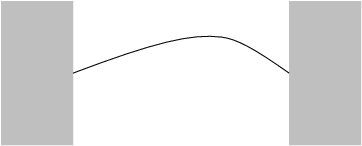
\epsfig{file={../fig/cordef},width=6 cm,angle=-90}}   
 \caption{La forme d'une corde fich\'ee entre deux murs peut \^etre
d\'ecrite par la solution 
d'un probl\`eme du type consid\'er\'e ici.}
 \label{figcordef}
\end{figure}
\begin{equation}
Lu=f\ {\rm dans}\ \Omega
\end{equation}
<\begin{equation}
u=0\ {\rm sur}\ \partial\Omega
\end{equation}
o\`u $L=\frac{\partial^{2}}{\partial x^{2}}$, $\Omega$ est le segment $[0,l]$
et $u$ repr\'esente l'\'ecart de la corde par rapport \`a l'\'equilibre. 
On montre que 
$\cal H$,
l'ensemble des fonctions nulles en $0$ et $l$ est un espace de Hilbert
pour le produit scalaire $\langle u,v \rangle=\int_0^lu(x)(x) dx$.
(On parle d'espace de {\bf Sobolev}, voir la section \ref{secexist}).
De plus on peut montrer que l'adjoint de $L$ est 
 $L^*=\frac{\partial^{2}}{\partial x^{2}}$.
\begin{equation}\label{eqadjoimq}
<Lu,v>=\int_0^l \frac{d^2u}{dx^2}vdx=
\int_0^lu\frac{d^2v}{dx^2}dx+[v\frac{du}{dx}-u\frac{dv}{dx}]^l_0 
\end{equation}
Comme $L^*=L$, on dit que $L$ est {\bf auto-adjoint}.
\end{exmp}
\begin{rem}
L'\'etude spectrale des op\'erateurs auto-adjoints est faite \`a la section
suivante. 
\end{rem}
\begin{exmp}
Consid\'erons une {\bf corde glissante} entre deux tiges verticales distantes
de $l$. 
Ce syst\`eme est sch\'ematis\'e dans la figure \ref{figcordeg}.
\begin{figure}[htb]
 \centerline{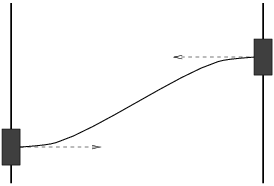
\epsfig{file={../fig/cordeg},width=6 cm,angle=-90}}   
 \caption{La forme assujettie \`a glisser le long de deux axes peut \^etre
d\'ecrite par la solution 
d'un probl\`eme du type consid\'er\'e ici.}
 \label{figcordeg}
\end{figure}
un tel syst\`eme physique peut \^etre mod\'elis\'e par les \'equations :
\begin{equation}
Lu=f\ {\rm dans}\ \Omega
\end{equation}
\begin{equation}
\frac{\partial u}{\partial n}=0\ {\rm sur}\ \partial\Omega
\end{equation}
o\`u, comme dans le cas pr\'ec\'edent, l'op\'erateur $L$ est 
$\frac{\partial^{2}}{\partial x^{2}}$, $\Omega$ est le segment $[0,l]$
et $u$ repr\'esente l'\'ecart de la corde par rapport \`a l'\'equilibre.
On montre que $\cal H_2$,
l'ensemble des fonctions de d\'eriv\'ee nulle en $0$ et $l$, est un
espace de Hilbert 
pour le produit scalaire $\langle u,v \rangle=\int_0^lu(x)(x) dx$.
En utilisant l'\'equation \ref{eqadjoimq}, on montre que $L$ est
encore auto-adjoint.
\end{exmp}


La forme :\index{forme d\'efinie}
\begin{equation}
<Lu,u>=\int_o^l\frac{d^2u}{dx^2}udx=
[u\frac{du}{dx}]_0^l-\int_0^l(\frac{df}{dx})^2dx=
-\int_0^l(\frac{df}{dx})^2dx 
\end{equation}
est une {\bf forme d\'efinie} n\'egative dans le cas de la corde fix\'ee et n\'egative
(non-d\'efinie) dans le cas de la corde glissante. Dans ce dernier cas
en effet, la fonction $u=cte$ annule  $<Lu,u>$.

Le choix des espaces est important aussi pour la {\bf compatibilit\'e
entre les donn\'ees $f$ et $g$}\cite{ma:equad:Dautray1,ph:elect:VanBladel75}.
le th\'eor\`eme suivant traite de ce probl\`eme :
\begin{thm}
Si il existe une solution non nulle $v_0$ pour le probl\`eme adjoint :
\begin{equation}
L^*v_0=0
\end{equation}
alors une condition n\'ecessaire pour que le probl\`eme $Lu=f$
poss\`ede une solution est que $f$ soit orthogonal \`a $v_0$. 
\end{thm}
\begin{pf}
Supposons qu'il existe une soultion $u_1$ au probl\`eme :
\begin{equation}
Lu=f
\end{equation}
Alors,
\begin{equation}
\forall v,\ <v,Lu_1>=<v,f>
\end{equation}
donc 
\begin{equation}
\forall v,\ <L^*v,u_1>=<v,f>
\end{equation}
Si il existe une fonction $v_0$ telle que $L^*v_0=0$ alors l'\'equation
pr\'ec\'edente implique :
\begin{equation}
<v_0,f>=0
\end{equation}
\end{pf}

\begin{exmp}
dans le cas de la corde glissante la fonction $v_0=1$ sur $[0,l]$ est solution
du probl\`eme adjoint. Notre condition de compatibilit\'e pr\'ec\'edente
devient : $f$ doit \^etre de moyenne nulle. En effet ici
\begin{equation}
<v_0,f>=\int_0^lf dx
\end{equation}


\end{exmp}

\begin{rem}
Nous reviendrons sur ces probl\`emes de compatibilit\'e lors de l'\'etudes des
m\'ethodes int\'egrales de la section \ref{chapmethint}.
\end{rem}
\section{Quelques th\'eor\`emes d'analyse spectrale}
%%%%%%%%%%%%%%%%%%%%%%%%%%%%%
Dans cette section, nous envisageons l'analyse spectrale d'un op\'erateur
lin\'eaire $L$. les r\'esultats pr\'esent\'es ici sont d\'emontr\'es dans le
cas o\`u $L$ est un op\'erateur d'un espace vectoriel $E$ de dimension fini
dans lui-m\^eme. Nous renvoyons le lecteur \`a l'abondanet litt\'erature sur
le sujet pour des espaces plus complexes (voir par exemple
\cite{ma:equad:Dautray5}). 
Soit $L$ un op\'erateur lin\'eaire agissant sur $E$.
Le probl\`eme spectral associ\'e \`a $L$ est :
\begin{prob}
Trouver les vecteurs $u\in V$ non-nuls  et les nombres $\lambda$ tels
que :
\begin{equation}
Lu=\lambda u
\end{equation}
\end{prob}
\begin{thm}
On a \'equivalence
\begin{enumerate}
\item $\exists u \neq 0 \: Lu=\lambda u$
\item la matrice $L-\lambda I$ est singuli\`ere
\item $det(L-\lambda I)=0$
\end{enumerate}
\end{thm}
Une matrice est dite diagonalisable si il existe une base dans
laquelle elle a une forme diagonale\cite{ma:algeb:Strang76}.
\begin{thm}
Si une matrice carr\'ee $L$ de dimension $n$ poss\`ede $n$ vecteurs propres
lin\'eairement ind\'ependants, alors $L$ est diagonalisable.
De plus si ces vecteurs sont choisis comme \'etant les colonnes d'une
matrice $S$ alors on a :
\begin{equation}
\Lambda = S^{-1} L S {\rm,\ avec\ \Lambda\  diagonale}
\end{equation}
\end{thm}
\begin{pf}
Mettons les vecteurs propres $u_i$ dans les colonnes de $S$ et
calculons $LS$ :
\begin{equation}
LS=L \left( \begin{array}{cccc}
              \vdots&\vdots& &\vdots\cr
               u_1&u_2&\ldots&u_n\cr 
              \vdots&\vdots& &\vdots\cr
\end{array} \right)
\end{equation}
\begin{equation}
=
\left( \begin{array}{cccc}
              \vdots&\vdots& &\vdots\cr
              \lambda_1 u_1&\lambda_2 u_2&\ldots&\lambda_n u_n\cr
              \vdots&\vdots& &\vdots\cr
\end{array} \right)
\end{equation}
\begin{equation}
\left( \begin{array}{cccc}
\vdots&\vdots& &\vdots\cr
              u_1&u_2&\ldots&u_n\cr
              \vdots&\vdots&
&\vdots\cr
\end{array} \right)
.
\left( \begin{array}{cccc}
\lambda_1& & &\cr
&\lambda_2&&\cr
&&\ddots&\cr
&&&\lambda_n
\end{array} \right)
\end{equation}
\begin{equation}
LS=S\Lambda
\end{equation}
Or $S$ est inversible car ses vecteurs sont supposes lin\'eairement
ind\'ependants.
\begin{equation}
\lambda=S^{-1}LS
\end{equation}
\end{pf}
\begin{rem}\label{remmatrindep}
Si une matrice $L$ a $n$ valeurs propres distinctes alors ses $n$
vecteurs propres sont lin\'eairement ind\'ependants.
\end{rem}

Supposons que $E$ est un espace de Hilbert.
\begin{defn}
L'op\'erateur $L^*$ adjoint de $L$ est par d\'efinition l'op\'erateur
d\'efini par 
\begin{equation} 
\forall u,\ v\  \ \langle L^*u|v\rangle = \langle u|Lv\rangle 
\end{equation}
\end{defn}
\begin{defn} 
Un op\'erateur auto-adjoint est un op\'erateur tel que $L=L^*$
\end{defn}
\begin{thm}
Pour chaque op\'erateur hermitique $A$, il existe au moins une base
constitu\'ee de ses vecteurs propres orthonorm\'es. Il est diagonal dans
cette base et les \'el\'ements diagonaux sont les valeurs propres.
\end{thm}
\begin{pf}
Consid\'erons un espace $E_n$ de dimension $n$. Soit  $|u_1\rangle $ le
vecteur propre associe \`a une valeur propre $\lambda_1$ de $A$.
Consid\'erons une base form\'ee par ($|u_1\rangle $ somme directe une base
quelconque de $E^\perp_{n-1}$).
Dans cette base  
\begin{equation}
L= 
\left( \begin{array}{cccc}
\lambda_1& &v& \cr
             0& & & \cr
             \vdots& &B& \cr
              0& & & \cr
\end{array} \right)
\end{equation}
La premi\`ere colonne de $L$ est l'image de $u_1$.
Or $L$ est hermitique donc :
\begin{equation}
L= 
\left( \begin{array}{cccc}
\lambda_1&0&\ldots&0 \cr
             0& & & \cr
             \vdots& &B& \cr
              0& & & \cr
\end{array} \right)
\end{equation}
Par r\'ecurrence, on montre la propri\'et\'e.
\end{pf}
\begin{thm}
Les valeurs propres d'un op\'erateur hermitique $L$ sont r\'eelles.
\end{thm}
\begin{pf}
\begin{equation}
L|u\rangle =\lambda|u\rangle 
\end{equation}
Multiplions par $ \langle u|$
\begin{equation}
 \langle u|Lu\rangle =\lambda \langle u|u\rangle 
\label{uAu}
\end{equation}
prenons la conjugu\'ee de l'\'equation \ref{uAu} 
\begin{equation}
 \langle u|L^*u\rangle =\lambda^* \langle u|u\rangle 
\end{equation}
$ \langle u|u\rangle $ \'etant un r\'eel et $L^*=L$, on a bien
$\lambda=\lambda^*$ 
\end{pf}
\begin{thm}
Deux vecteurs propres $|u_1\rangle $ et $|u_2\rangle $ associ\'e \`a deux
valeurs 
propres distinctes $\lambda_1$ et $\lambda_2$ d'un op\'erateur
hermitique sont orthogonaux.
\end{thm}
\begin{pf}
\begin{equation}
L|u_1\rangle =\lambda_1|u_1\rangle 
\end{equation}
\begin{equation}
L|u_2\rangle =\lambda_2|u_2\rangle 
\end{equation}
D'o\`u :
\begin{equation}
 \langle u_2|Lu_1\rangle =\lambda_1 \langle u_2|u_1\rangle 
\end{equation}
\begin{equation}
 \langle u_1|Lu_2\rangle =\lambda_2 \langle u_1|u_2\rangle 
\end{equation}
En faisant la diff\'erence des deux \'equations pr\'ec\'edentes :
\begin{equation}
0=(\lambda_1-\lambda_2) \langle u_2|u_1\rangle 
\end{equation}
\end{pf}

Apr\`es ces quelques rappels, voici les principales strat\'egies que nous
utiliserons pour r\'esoudre les probl\`emes pr\'esent\'es dans la premi\`ere
section de ce chapitre.

\section{M\'ethodes Int\'egrales}\label{chapmethint}
%%%%%%%%%%
\subsection{Fonction de Green}
%%%%%%%%%%%%
les m\'ethodes int\'egrales sont utilis\'ees pour r\'esoudre les probl\`emes
(aux limites) lin\'eaires. La lin\'earit\'e est ici essentielle; la d\'emarche
consiste \`a affirmer que si l'on connait les r\'eponse $u_i$ d'un syst\`eme
physique 
lin\'eaire $L$ \`a des entr\'ees $f_i$ alors on connait la r\'eponse $u$ de ce
syst\`eme \`a une entr\'ee $f$ qui est une somme de $\sum c_i f_i$ (o\`u les
$c_i$ des r\'eels).

On trouve des applications de cette m\'ethode dans la th\'eorie de la
diffraction (voir la section \ref{secdiffra}). Les solutions \'el\'ementaires
sont tr\`es utilis\'ees dans les probl\`emes d'\'electrostatique
(voir \ref{secpotelec}).
 
Consid\'erons (\cite{ph:elect:VanBladel75,ma:equad:Dautray2})
le probl\`eme $P(f,\phi,\psi)$
\begin{prob}\label{probpfppgreen}(probl\`eme $P(f,\phi,\psi)$) :
Trouver $u$ tel que :
\begin{equation}
 Lu=f\ {\rm dans}\ \Omega
\end{equation}
\begin{equation}
u=\phi\ {\rm sur}\ \partial \Omega_1
\end{equation}
\begin{equation}
\frac{\partial u}{\partial n_{L}}=\psi\ {\rm sur}\ \partial \Omega_2
\end{equation}
avec $\partial \Omega_1 \cup\partial \Omega_2=\partial \Omega$.
\end{prob}
Pour r\'esoudre ce probl\`eme nous allons employer la m\'ethode de
Green. 

\subsubsection{Cas o\`u le noyau est nul, Probl\`eme homog\`ene}
%%%%%%%%%%%%%
\begin{defn}\label{defgreen}
On appelle solution de Green\index{Green (solution de)} du probl\`eme $P(f,0,0)$ la fonction
${\cal G}_y(x)$ solution de 
\begin{equation}
L{\cal G}_y=\delta_y
\end{equation}
On appelle solution de Green du probl\`eme adjoint $P(f,0,0)$ la fonction
${\cal G}^*_y(x)$ solution de 
\begin{equation}
\overline{L^*{\cal G}^*}_y=\delta_y
\end{equation}
o\`u la barre horizontale repr\'esente la conjugaison complexe.
\end{defn}
\begin{thm}\label{theogreen}
Si ${\cal G}_y$ et ${\cal G}^*_y$ existent alors 
$\overline{{\cal G}^*}_y(x)= {\cal G}_x(y)$
\end{thm}
\begin{pf}
Par d\'efinition de l'adjoint $L^*$ d'un op\'erateur $L$
\begin{equation}
\int \overline{L^*{\cal G^*}}_y(r){\cal G}_x(r)= \int \overline{{\cal
G^*}}_{y}(r)L{\cal G}_x(r) 
\end{equation}
En utilisant les relation de d\'efinition \ref{defgreen}
 de ${\cal G}_y$ et ${\cal G}^*_y$
on obtient le r\'esultat.
\end{pf}
En particulier si $L=L^*$ alors ${\cal G}^*_x(y)= {\cal G}_x(y)$.

\begin{thm}
Il existe une unique fonction ${\cal G}_y$ telle que
\begin{equation}
u(y)=\int {\cal G}_x(y) f(x)dx
\end{equation}
soit solution du probl\`eme $P(f,0,0)$ 
et
\begin{equation}
L{\cal G}_y=\delta_y
\end{equation}
\end{thm}
On ne d\'emontre pas ici ce th\'eor\`eme (existence) mais remarquons
que si 
${\cal G}_y$ existe alors on a bien :
\begin{equation}
u(y)=\int \delta_y(x)u(x)=\int \overline{L^*{\cal G}^*}_y(x) u(x)dx,
\end{equation}
soit, par d\'efinition de l'op\'erateur adjoint 
\begin{equation}
u(y)=\int \bar{\cal G}^*_y(x) Lu(x)dx.
\end{equation}
En utilisant la relation $Lu=f$ :
\begin{equation}
u(y)=\int \bar{\cal G}^*_y(x) f(x),
\end{equation}
qui est d'apr\`es le th\'eor\`eme \ref{theogreen}
\begin{equation}
u(y)=\int {\cal G}_x(y) f(x)dx
\end{equation}
Cette derni\`ere \'equation permet de trouver la solution du probl\`eme
aux limites, pour toute fonction $f$, une fois la fonction de Green
${\cal G}_x(y)$ connue.

\subsubsection{Noyau nul, Probl\`eme non-homog\`ene}
%%%%%%%%%%%%%
La solution du probl\`eme $P(f,\phi,\psi)$ s'obtient 
aussi \`a partir des fonctions de Green pr\'ec\'edentes :
\begin{equation}
u(y)=\int \delta_y(x)u(x)=\int \overline{L^*{\cal G^*}}_y(x)u(x)dx.
\end{equation}
En appliquant le th\'eor\`eme de Green, on a :
\begin{equation}
u(y)=\int \bar{\cal G}^*_y(x) Lu(x)dx
+\int_\Gamma  (\bar{\cal G}^*_y\frac{\partial u}{\partial
n}-u\frac{\partial \bar{\cal G}^*_y}{\partial n}),
\end{equation}
et en utilisant les conditions aux limites, et le r\'esultat du
th\'eor\`eme \ref{theogreen}, on obtient :
\begin{equation}
u(y)=\int {\cal G}_x(y) f(x)+\int_\Gamma  ({\cal
G}_x(y)\phi-\psi\frac{\partial {\cal G}_x(y)}{\partial n}), 
\end{equation}
Cette derni\`ere \'equation permet de trouver la solution du probl`eme
aux limites, pour toute fonction $f,\phi,\psi$, une fois la fonction
de Green 
${\cal G}_x(y)$ connue.


\subsubsection{Cas o\`u le noyau est non-nul, Probl\`eme homog\`ene}
%%%%%%%%%%%%%
Nous retrouvons ici le th\'eor\`eme de la section \ref{secchoixesp} :
\begin{thm}
Si  $Lu_0=0$ a des solutions non-nulles et si $f$ n'est pas
dans l'orthogonal de $Ker(L^*)$, alors le probl\`eme 
$P(f,0,0)$ n'a pas de
solution.
\end{thm}
\begin{pf}
Supposons qu'il existe une solution $u$ de $Lu=f$. Soit $v_0$ une
solution quelconque de $L^*v_0=0$ (i.e un vecteur quelconque de
$Ker(L^*)$).
Alors :
\begin{eqnarray}
 \langle f|v_0\rangle &=& \langle Lu,v_0\rangle  \nonumber\\
       &=& \langle u,L^*v_0\rangle 
\end{eqnarray} 
D'o\`u $ \langle f|v_0\rangle =0$
\end{pf}

Mais 
en se pla\c cant dans l'orthogonal du noyau de $L$, on contourne ce probl\`eme
et on peut refaire des calculs similaires au cas pr\'ec\'edent.
Supposons que le noyau de $L$ soit engendr\'e par $u_0$ et le noyau de
$L^*$ soit engendr\'e par $v_0$.
\begin{defn}\label{defgreen2}
On appelle solution de Green du probl\`eme $P(f,0,0)$ la fonction
${\cal G}_y(x)$ solution de 
\begin{equation}
L{\cal G}_y=\delta_y-u_0(y)u_0
\end{equation}
On appelle solution de Green du probl\`eme adjoint $P(f,0,0)$ la fonction
${\cal G}^*_y(x)$ solution de 
\begin{equation}
\overline{L^*{\cal G}^*}_y=\delta_y-v_0(y)v_0
\end{equation}
 o\`u la barre horizontale repr\'esente la conjugaison complexe.
\end{defn}
\begin{thm}\label{theogreen2}
Si ${\cal G}_y$ et ${\cal G}^*_y$ existent alors 
$\overline{{\cal G}^*}_y(x)= {\cal G}_x(y)$
\end{thm}
\begin{pf}
Par d\'efinition de l'adjoint $L^*$ d'un op\'erateur $L$
\begin{equation}
\int \overline{L^*{\cal G^*}}_y(r){\cal G}_x(r)dr=\int \overline{{\cal G^*}}_{y}(r)L{\cal G}_x(r)dr
\end{equation}
En utilisant les relations de d\'efinition \ref{defgreen2}
 de ${\cal G}_y$ et ${\cal G}^*_y$
on obtient le r\'esultat.
\end{pf}
En particulier si $L=L^*$ alors ${\cal G}^*_x(y)= {\cal G}_x(y)$.
\begin{thm}
Il existe une unique fonction ${\cal G}_y$ telle que
\begin{equation}
u(y)=\int {\cal G}_x(y) f(x)dx
\end{equation}
soit solution du probl\`eme $P(f,0,0)$ dans $Ker(L)^\perp$ 
et
\begin{equation}
L{\cal G}_y=\delta_y-u_0(y)u_0
\end{equation}
\end{thm}
On ne d\'emontre pas ici ce th\'eor\`eme (existence). Justifions
n\'eanmoins la formule de d\'efinition de la solution.
Supposons que ${\cal G}_y$ existe .
Soit $u_c$ la projection d'une fonction $u$ sur  $Ker(L)^\perp$.
\begin{equation}
u_c(y)=u(y)-u_0(y)\int \bar{u}_0(x)u(x) dx
\end{equation}
qui s'\'ecrit aussi :
\begin{equation}
u_c(y)=\int \delta_y(x)u(x)-u_0(y)\int \bar{u}_0(x)u(x) dx,
\end{equation}
ou
\begin{equation}
u_c(y)=\int \overline{L^*{\cal G}^*}_y(x) u(x)dx=\int \bar{\cal G}^*_y(x) Lu(x)dx=\int \bar{\cal G}^*_y(x) f(x)
\end{equation}
qui est d'apr\`es le th\'eor\`eme \ref{theogreen2}
\begin{equation}
u_c(y)=\int {\cal G}_x(y) f(x)dx
\end{equation}

\subsection{R\'esolution}
%%%%%%%%%%%%%%%%%%%%%%%%%%
Une fois la fonction de Green d'un probl\`eme trouv\'ee, la solution au
probl\`eme s'obtient par simple int\'egration.
L'utilisation des sym\'etries permet de simplifier la recherche des fonctions
de Green.

\subsubsection{M\'ethode des images}\index{images (m\'ethodes des)}
%%%%%%%%%
Soit $U$ un domaine pr\'esentant un plan de sym\'etrie : $\forall x
\in U, -x\in U$. Soit $\partial U$ le bord de $U$.
Le plan de sym\'etrie s\'epare $U$ en deux sous-domaines : $U_1$ et
$U_2$ (voir la figure \ref{figsymet}).
\begin{figure}[htb]
 \centerline{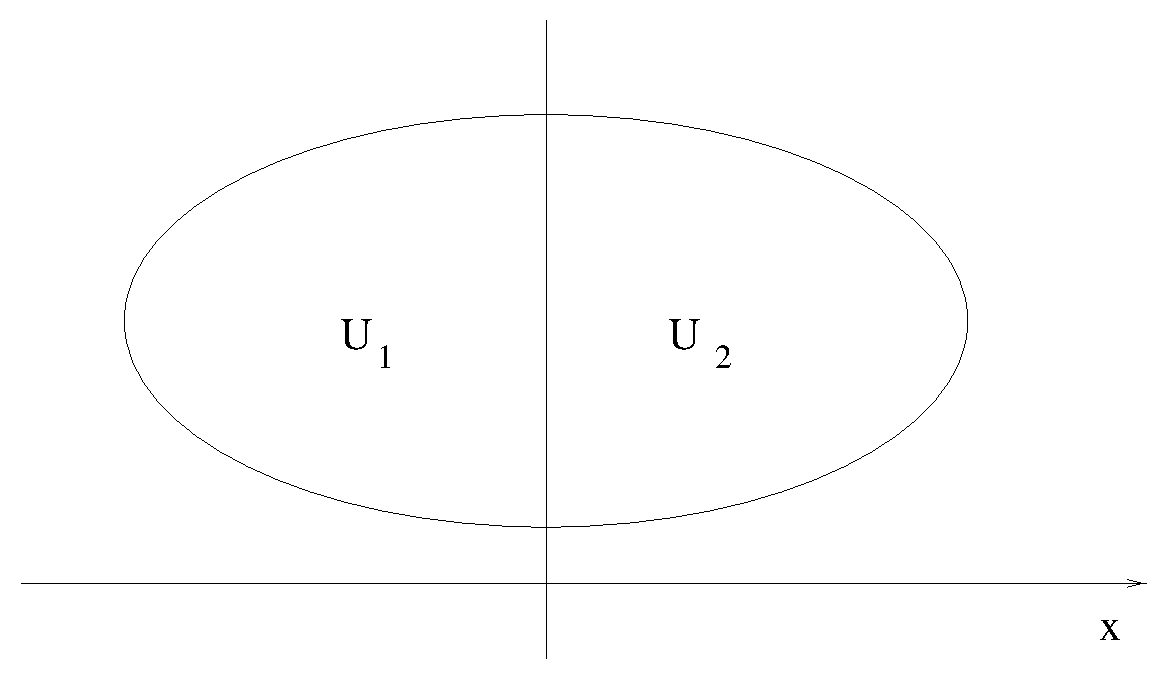
\epsfig{file={../fig/symet},width=6 cm,angle=-90}}   
 \caption{Le domaine $U$ est l'union des domaines $U_1$ et $U_1$
sym\'etriques par rapport au plan $x=0$.}
 \label{figsymet}
\end{figure}
Nous nous proposons de chercher la solution du probl\`eme
\begin{prob}\label{probori} 
Trouver $G_y(x)$ telle que :
\begin{equation}
LG_y(x)=\delta(x)\ {\rm dans}\ U_1
\end{equation}
et
\begin{equation}
 G_y(x)=0 {\rm \ sur\ } \partial U_1
\end{equation}
\end{prob}
connaissant la solution du probl\`eme
\begin{prob}\label{probconnu}
Trouver $G^1_y(x)$ telle que :
\begin{equation}
LG^U_y(x)=\delta(x) {\rm \ sur\ } U
\end{equation}
et
\begin{equation}
 G^U_y(x)=0 {\rm \ sur\ } \partial U
\end{equation}
\end{prob}
R\'esoudre le probl\`eme \ref{probori} en passant par le probl\`eme
\ref{probconnu} est connu
sous le nom de m\'ethode des images voir \cite{ma:equad:Dautray2} page 655
Posons ${\cal G}_y(x)={G}^U_y(x)-{G}^U_y(-x)$. La fonction ${\cal
G}_y(x)$ v\'erifie  
\begin{equation}
L{\cal G}_y(x)=\delta(x)\ {\rm dans}\ U_1
\end{equation}
et
\begin{equation}
{\cal G}_y(x)=0 {\rm \ sur\ } \partial U_1
\end{equation}
Les fonctions ${\cal G}_y(x)$ et $G_y(x)$ v\'erifient la m\^eme
\'equation. La fonction de Green $G_y(x)$ 
est donc simplement la 
restriction de la fonction ${\cal G}_y(x)$ \`a $U_1$.
Nous avons donc r\'esolu le probl\`eme \ref{probori}.

\subsubsection{Invariance par translation}
%%%%%%
Lorsque probl\`eme $P(f,0,0)$ est invariant par translation
la relation fonction de Green ${\cal G}_y(x)$ devient
une fonction qui ne d\'epend que de la diff\'erence $x-y$.
La relation int\'egrale donnant la solution du probl\`eme
devient une relation de convolution :
\begin{equation}
u(x)=\int {\cal G}(x-y)f(y)dx={\cal G}*f
\end{equation}
${\cal G}$ est appel\'ee  solution \'el\'ementaire et est not\'ee $e$.
Le cas o\`u $P(f,0,0)$ est invariant par translation
correspond typiquement au cas o\`u les fronti\`eres sont  \`a
l'infini\cite{ma:distr:Petit91}. 
Donnons les solutions \'el\'ementaires de quelques probl\`emes
classiques :
\begin{exmp}
\'Equation de Laplace dans $R^3$. L'op\'erateur consid\'er\'e est 
\begin{equation}
L=\Delta
\end{equation}
La solution \'el\'ementaire est :
\begin{equation}
e(r)=\frac{1}{4\pi r}
\end{equation}
\end{exmp}
\begin{exmp}
\'Equation de Helmholtz dans $R^3$. L'op\'erateur consid\'er\'e est 
\begin{equation}
L=\Delta+k^2
\end{equation}
La solution \'el\'ementaire est :
\begin{equation}
e(r)=\frac{e^{jkr}}{4\pi r}
\end{equation}
\end{exmp}

\section{M\'ethodes variationnelles}\label{chapmetvar}
%%%%%%%%%%%%%%%%%%%%%%
\subsection{Les diff\'erents probl\`emes de minimisation de fonctionnelles}
%%%%%%%%%%%%%%
Nous avons vu \`a la section \ref{secexist} que la formulation
variationelle \'etait tr\`es utile pour montrer l'existence et
l'unicit\'e de probl\`emes aux limites.
Mais de nombreux principes physiques s'\'ennoncent naturellement sous une
forme variationnelle. 
C'est le cas du principe de moindre action en m\'ecanique (voir la section
 \ref{secprinmoindreact}), du principe des puissances virtuelles (voir la
section  \ref{secpuisvirtu}) en m\'ecanique, du principe de
Fermat en optique (voir la section \ref{secFermat}) et du principe fondamental
de la physique statistique (voir le chapitre \ref{chapphysstat}).

Dans cette section, nous allons  pr\'eciser les
diff\'erents type de probl\`emes variationnels rencontr\'es en
physique.

Comme \`a la section \ref{secexist}, on se donne :\index{maximisation}
\begin{itemize}
\item un espace de Hilbert $V$ de norme $\|\ .\ \|$;
\item une forme bilin\'eaire $a$ : $u,v\rightarrow a(u,v)$ continue
sur $V\times V$
\item une forme lin\'eaire $L$ : $v\rightarrow L(v)$ continue sur $V$.
\end{itemize}
On consid\`ere le probl\`eme :
\begin{prob}\label{provari2} 
Trouver $u\in V$ tel que 
\begin{equation}
\forall v\in V, a(u,v)=L(v)
\end{equation}
\end{prob}
On a vu (th\'eor\`eme de Lax-Milgram) que
si la forme bilin\'eaire $a$ est $V$-elliptique
alors le probl\`eme pr\'ec\'edent admet une solution unique.
Supposons maintenant que la forme $a(u,v)$ est sym\'etrique,
c'est-\`a-dire que 
\begin{equation}
\forall u\in V,\ \forall v\in V,\ a(u,v)=a(v,u).
\end{equation}
Introduisons la fonctionnelle quadratique :
\begin{equation}
J(v)=\frac{1}{2}a(v,v)-L(v)
\end{equation}
Consid\'erons le probl\`eme :
\begin{prob}\label{promini}
Trouver $u\in V$, tel que :
\begin{equation}
J(u)=\min_{v\in V} J(v)
\end{equation}
\end{prob}
On montre le th\'eor\`eme suivant :
\begin{thm}
La solution du probl\`eme \ref{promini} existe et est unique. De plus
c'est la solution du probl\`eme \ref{provari2}.
\end{thm}
Donnons quelques exemples d'ensemble $V$.
\begin{exmp}
Si on prend :
\begin{equation}
V=\{v\in U, \phi_{i}(v)=0,\ i\in 1,\dots,n \}
\end{equation}
o\`u les $\phi_{i}(v)$ sont $n$ fonctionnelles.
On tombe alors sur un probl\`eme de minimisation de fonctionnelle avec
contraintes \cite{ma:equad:Ciarlet88},\index{contrainte} sur les
multiplicateurs de Lagrange. 
\end{exmp}
\begin{exmp}
Si on prend :
\begin{equation}
V=\{v\in U, \phi_{i}(v)\leq 0,\ i\in 1,\dots,n  \}
v\end{equation}
o\`u les $\phi_{i}(v)$ sont $n$ fonctionnelles.
Il s'agit d'un autre type de contrainte.
\end{exmp}
On peut interpr\'eter un probl\`eme sans contrainte par le sch\'ema
de la figure \ref{figcontraintesans}
\begin{figure}[htb]
 \centerline{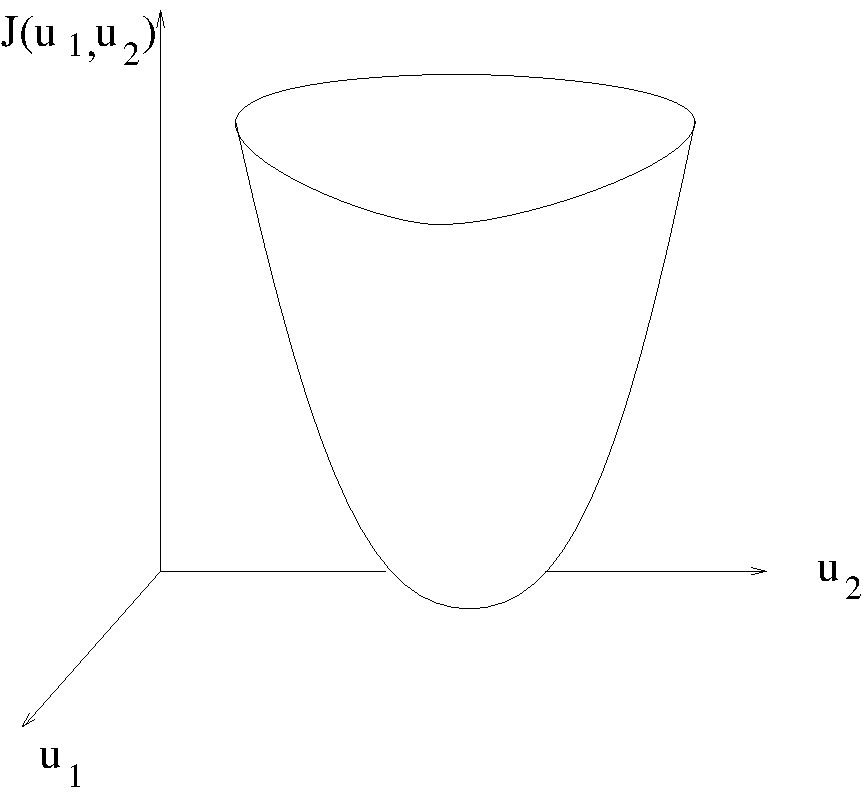
\epsfig{file={../fig/contraintesans},width=6 cm,angle=-90}}   
 \caption{Minimisation d'une fonctionelle sans contrainte. Dans le cas
o\`u l'espace fonctionnel est \`a deux dimensions, on peut
repr\'esenter $J$ par une surface.}
 \label{figcontraintesans}
\end{figure}
On peut interpr\'eter un probl\`eme avec
contraintes\cite{ma:equad:Ciarlet88} par le sch\'ema 
de la figure \ref{figcontrainteavec}.
\begin{figure}[htb]
 \centerline{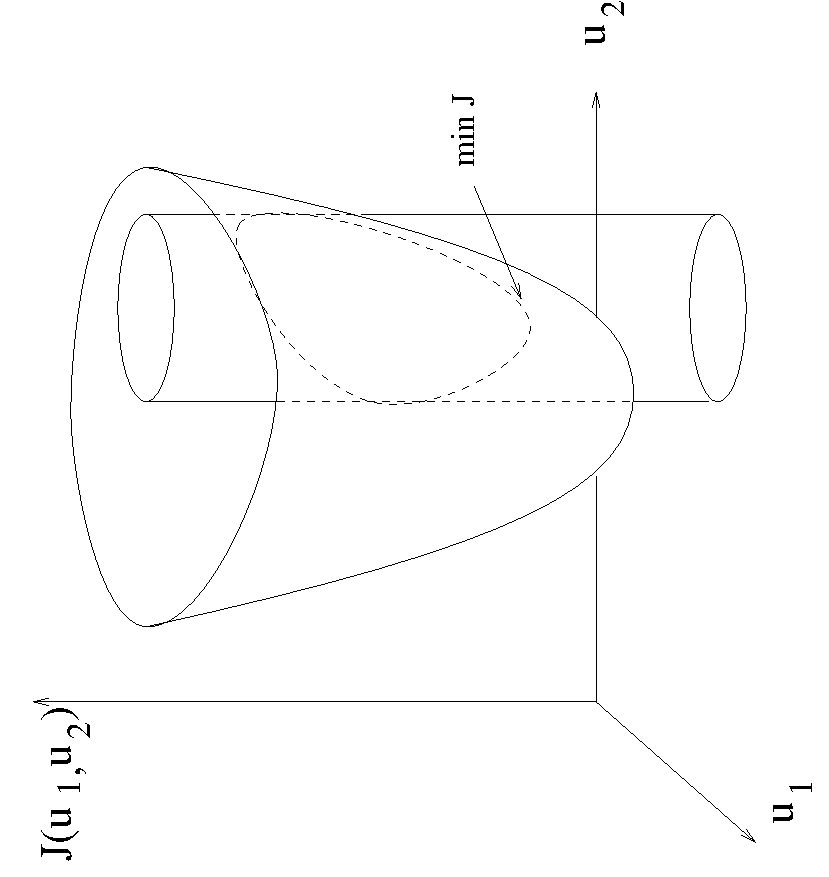
\epsfig{file={../fig/contrainteavec},width=6 cm,angle=-90}}   
 \caption{Minimisation d'une fonctionelle avec contrainte. L'espace
fonctionnel est \`a deux dimensions. La contrainte est ici la
r\'eduction de l'espace des $u_i$ accessible \`a un disque dans les plan
$u_1,u_2$. }
 \label{figcontrainteavec}
\end{figure}


 Le lien avec les \'equations au d\'eriv\'ees partielles a
\'et\'e trait\'e \`a la section \ref{secexist} : \`a un probl\`eme
d'\'equations au 
d\'eriv\'ees partielles correspond un probl\`eme variationnel. 
Nour reviendrons sur ce probl\`eme \`a l'occasion du principe de
moindre-action (\'equivalence entre le principe de moindre action et la
relation fondamentale de la dynamique - voir la section
\ref{secprinmoindreact} ) ainsi qu'\`a
l'occasion de l\'etude du principe des
puissances virtuelles (comment relier la formulation variationelle aux
\'equations locales de la dynamique des milieux continus - voir
\ref{secpuisvirtu}).

\subsection{Approximation de probl\`emes variationnels}
%%%%%%%%%%%
La r\'esolution d'un probl\`eme variationnel peut se faire de mani\`ere
num\'erique. On se ram\`ene alors a la r\'esolution de syst\`emes
d'\'equations (voir la section \ref{secvarinum}) en approchant les espaces
fonctionnels. 
Il existe de nombreuses autres m\'ethodes de r\'esolution num\'erique
particuli\`erement d\'edi\'es aux
probl\`emes d'optimisation : m\'ethodes de relaxation,
de gradient pour des probl\`emes avec ou sans contraintes.
Pour une \'etude de ces m\'ethodes nous renvoyons \`a \cite{ma:equad:Ciarlet88}.


Une approche int\'eressante sur le plan th\'eorique (voir le chapitre
\ref{chapphysstat})  est celle des {\bf multiplicateurs de Lagrange}.
Cette m\'ethode n'est pas directement adapt\'ee au probl\`eme de
minimisation d'une fonctionelle mais plut\^ot au probl\`eme de
minimisation d'une fonction d'un nombre $N$ de variable avec
contrainte.\index{contrainte}\index{Lagrange (multiplicateur de)}
\begin{prob}
Trouver le point $x$ de l'espace $V$ de dimension $N$ tel que 
\begin{equation} 
F(x)=\min_{y\in V}F(y)
\end{equation}
avec les contraintes $n$, $R_i(x)=0,\ i=1,\dots,n.$
\end{prob}
Dans un probl\`eme sans contrainte on sait qu'une solution $x$
v\'erifie 
\begin{equation}
dF=0
\end{equation}
Dans le cas de la pr\'esence de contraintes, les $n$ coordonn\'ees
$x_i$ de $x$ ne sont pas ind\'ependantes. En effet elles doivent aussi
v\'erifier les relations
\begin{equation}
dR_i=0
\end{equation}
La m\'ethode de Lagrange consiste \`a chercher $n$ nombres $\lambda_i$
appel\'es multiplicateurs de Lagrange tels que 
\begin{equation}
dL=dF+\sum \lambda_i dR_i=0
\end{equation}
On obtient donc un syst\`eme d'\'equation :
\begin{equation}
\frac{\partial F}{\partial x_j}+\sum \lambda_i \frac{\partial R_i}{\partial x_j}=0
\end{equation}
\begin{exo}\label{exoentr}
Consid\'erons le probl\`eme de maximisation de l'entropie 
\begin{equation}
S=-k_B\sum_{(l)}P_l\ln P_l
\end{equation}
avec les $n+1$ contraintes 
\begin{equation}
R_0=\sum P_l-1=0
\end{equation}
\begin{equation}
R_i=\sum X^i_lP_l-\bar X^i=0,\ i=1,\dots,n
\end{equation}
Trouver, en utilisant la m\'ethode des multiplicateurs de Lagrange la
distribution des $P_l$ solution de ce probl\`eme de maximisation.
\end{exo}
(voir solution en annexe)


\section{M\'ethode Spectrale, \'evolution lin\'eaire}\label{chapmethspec}
%%%%%%%%%%%%%%%%%%%%%%%%%%%%%%%%
\subsection{Point de vue spectral}
%%%%%%%%%%%%%%%%%%%%%%

La m\'ethode spectrale est une m\'ethode utilis\'ee pour r\'esoudre les
probl\`emes d'\'evolution lin\'eaires du type probl\`eme \ref{probevollin}.
La m\'ecanique quantique (voir les chapitres \ref{chapmq} et
\ref{chapproncorps} ) fournit de tr\`es 
beaux probl\`emes spectraux 
{\it via} l'\'equation de Schr\"odinger.
Les valeurs propres de l'op\'erateur lin\'aire consid\'er\'e (l'hamiltonien)
sont interpr\'et\'ees comme les \'energies associ\'ees \`a des \'etats (les
vecteurs propres de l'hamiltonien).
L'\'electromagn\'etisme aussi conduit souvent  \`a des
probl\`emes spectraux (modes de cavit\'es)


le probl\`eme suivant est un cas particulier du probl\`eme lin\'eaire
d'\'evolution  \index{r\'eponse lin\'eaire} (on parle alors de {\bf r\'eponse
  lin\'eaire}) 
\begin{prob} 
Trouver $\phi\in V$ tel que :
\begin{equation}
\frac{d\phi}{dt}=(H_0+H(t))\phi
\end{equation}
o\`u $H_0$ est un op\'erateur lin\'eaire  diagonalisable 
et $H(t)$ est  un op\'erateur lin\'eaire
``petit'' par rapport \`a $H_0$.
\end{prob}
ce probl\`eme peut aussi  \^etre abord\'e par une
m\'ethode spectrale.
Nous verrons \`a la section \ref{secreplinmq} un exemple de r\'eponse
  lin\'eaire en m\'ecanique quantique.



La m\'ethode spectrale consiste d'abord \`a d\'efinir proprement l'espace dans
lequel $L$ du probl\`eme  \ref{probevollin} agit 
et \`a le munir de la structure d'espace hilbertien.
On cherche alors les vecteurs tels que :
\begin{equation}
Lu_k(x)=\lambda_k(t)u_k(x)
\end{equation}
Une fois les fonctions propres $u_{k(x)}$ trouv\'ees, le probl\`eme est
r\'eduit \`a l'int\'egration d'un syst\`eme (diagonal) d'\'equations
diff\'erentielles ordinaires.



%%%%%%%%%%%%%%%%%%%%%%%%%%%%%%%%%%%%%%%%%%%%%%%%%%%%
\subsection{R\'esolution de probl\`emes spectraux}\label{chapresospec}
%%%%%%%%%%%%%%%%%%%%%%%%%%%%%%%%%%%%%%%%%%%%%%%%%%%
Une fois le probl\`eme spectral r\'esolu, on
 projette alors l'\'equation de d\'epart sur la base des
$u_k$  et on se trouve ramen\'e \`a un probl\`eme d'\'equation aux
d\'eriv\'ees ordinaires.
L'objet de cette section est de pr\'esenter quelques id\'ees pour la
r\'esolution du probl\`eme spectral.
Deux cas sont favorables : celui o\`u le probl\`eme pr\'esente des sym\'etries
et celui pour lequel une approche perturbative est envisageable.

\subsubsection{Utilisation des sym\'etries}
%%%%%%%%%%%%%%%%%%%%%%%%%%%%
L'utilisation des sym\'etries repose sur le th\'eor\`eme fondamental suivant :
\begin{thm}
Si $L$ commute avec un op\'erateur $T$, alors les vecteurs propres de $T$ sont
aussi vecteurs propres de $L$. 
\end{thm}
ce th\'eor\`eme est d\'emontr\'e dans l'annexe \ref{chapgroupes}.

Des applications de l'invariance par rotation peuvent \^etre trouv\'ees \`a la
section \ref{secpotcent}.
L'invariance par translation fait l'objet du th\'eor\`eme de Bloch
\ref{theobloch} que nous verrons \`a la 
section\ref{sectheobloch} donne des relations sur les vecteurs propres
d'un hamiltonien invariant par translation.

\subsubsection{Approximation perturbative}
%%%%%%%%%%%%%%%%%%%%%%%%%%%%%%%%%%%%%%%%%%
Une approximation perturbative  de la solution d'un probl\`eme spectral peut
\^etre envisag\'e \`a chaque fois que l'op\'erateur $U$ \`a diagonaliser peut
\^etre consid\'erer comme la somme d'un op\'erateur $U^{0} $que l'on sait
diagonaliser 
et d'un autre op\'erateur $U^{1}$ petit par rapport a $U^{0}$.


Nous cherchons donc \`{a} r\'{e}soudre le probl\`{e}me  suivant
:\index{perturbations pour les probl\`emes spectraux}
\begin{equation} 
U\mid  \phi \rangle  = \lambda\mid  \psi \rangle \label{bod}
\end{equation}

Nous introduisons le param\`etre $\epsilon$ et nous supposons que $U$
 se d\'{e}veloppe en $\epsilon$ :
\begin{equation} 
U=U_{0}+\epsilon U_{1}+\epsilon ^{2}U_2+...
\end{equation}

Nous admettons\footnote{ceci n'est pas \'evident d'un point de vue
math\'ematique (voir~{Kato}~\cite{ma:equad:Kato66})} que les vecteurs propres
se d\'eveloppent en $\epsilon$ :
pour le i$^{\grave eme}$ vecteur propre :
\begin{equation} 
\mid \phi^{i}\rangle =\mid \phi^{i}_{0}\rangle +\epsilon
\mid \phi^{i}_{1}\rangle +\epsilon^{2}\mid \phi^{i}_{2}\rangle +...
\label{hyph} 
\end{equation}

L' \'equation de d\'efinition (\ref{bod})  ne d\'etermine
les vecteurs propres qu'\`a un facteur pr\`es. 
En effet si $\mid \phi^{i}\rangle $ 
est solution du probl\`eme alors
$a\,e^{i\theta}\mid \phi^{i}\rangle $ est aussi
solution. 
Nous allons donc fixer la norme des vecteurs propres \`a $1$.
Nous pouvons aussi choisir la phase. Pour nos calculs nous imposons
simplement que la phase de $\mid \phi^{i}\rangle $ soit celle du vecteur
$\mid \phi^{i}_0\rangle $.

Les vecteurs propres approches $\mid \phi^{i}\rangle $ et 
$\mid \phi^{j}\rangle $ doivent
\^etre exactement orthogonaux .
\begin{equation} 
\langle \phi^{i}\mid \phi^{j}\rangle =0 
\end{equation}
En \'egalant les coefficients en $\epsilon^k$ on obtient :
\begin{equation}
\langle \phi^{i}_{0}\mid \phi^{j}_{k}\rangle +\langle \phi^{i}_{1}\mid
\phi^{j}_{k-1}\rangle +\ldots+\langle \phi^{i}_{k}\mid
\phi^{j}_{0}\rangle =0 
\end{equation}
%
Pour la suite, nous appelons cette \'equation, H(k;i,j) o\`u k
repr\'esente l'ordre, i et j les num\'eros des vecteurs.


Nous imposons aux vecteurs propres approches $\mid \phi^{i}\rangle $ 
d'\^etre exactement normes, et
$\langle \phi^{i}_{0}\mid \phi^{i}_{j}\rangle $ r\'eel :
\begin{equation} 
\langle \phi^{i}_{0}\mid \phi^{i}_{1}\rangle =1 
\end{equation}
En \'egalant le coefficient de $\epsilon^k$ avec $k > 1$ 
dans le produit
$\langle \phi^{i}\mid \phi^{i}\rangle =1 $ :
\begin{equation}
\langle \phi^{i}_{0}\mid \phi^{i}_{k}\rangle +\langle \phi^{i}_{1}\mid \phi^{i}_{k-1}\rangle +\ldots+\langle \phi^{i}_{k}\mid \phi^{i}_{0}\rangle =0
\end{equation}
Nous appelons cette \'equation N(i;k).


Portons les d\'eveloppements des vecteurs propres dans l'\'equation
spectrale \ref{bod} et \'egalons les coefficients des puissances 
successives de $\epsilon$ :
\begin{eqnarray}
&&U_{0}\mid \phi^{i}_{j}\rangle +U_{1}\mid \phi^{i}_{j-1}\rangle +...+U_{j}\mid \phi^{i}_{0}\rangle \nonumber\\
&=&\lambda_{0}^{i}\mid \phi^{i}_{j}\rangle +\lambda_{1}^{i}\mid \phi^{i}_{j-1}\rangle +...
+\lambda_{j}^{i}\mid \phi^{i}_{0}\rangle  \label{oivj}
\end{eqnarray}
Nous appelons ces \'equations E(k;j).

En projetant les \'equations pr\'ec\'edentes E(k;j) sur les vecteurs \`a
l'ordre 
z\'ero, et en utilisant les conditions pr\'ec\'edentes N(i;k),
on obtient successivement les corrections aux valeurs et vecteurs propres.

\subsubsection{Approximation variationnelle}
%%%%%%%%%%%%%%%%%%%%%%%%%%%%%%
De la m\^eme mani\`ere qu'un probl\`eme
\begin{prob}
Trouver $u$ telle que :
\begin{enumerate}
\item 
\begin{equation}
Lu=f,\ u\in E, x\in\Omega
\end{equation}
\item $u$ v\'erifie des conditions aux limites  sur le bord
$\partial 
\Omega$ de $\Omega$.
\end{enumerate}
\end{prob}
peut \^etre ramen\'e \`a la r\'esolution d'un prob\`eme variationel,
le probl\`eme est le probl\`eme spectral : 
\begin{prob}
Trouver $u$ et $\lambda$ tels que :
\begin{enumerate}
\item 
\begin{equation}
Lu-\lambda u=f,\ u\in E, x\in\Omega
\end{equation}
\item $u$ v\'erifie des conditions aux limites sur le bord $\partial
\Omega$ de $\Omega$.
\end{enumerate}
\end{prob}
peut lui aussi \^etre ramen\'e \`a un probl\`eme variationnel.
Dans le cas o\`u $L$ est autoadjoint et $f$ est nulle (cas de la
m\'ecanique quantique), on tombe sur un probl\`eme de minimisation. En
particulier on montre que:
\begin{thm}
Le vecteur propre $\phi$ d'\'energie la plus petite $E_0$  de
l'op\'erateur autoadjoint 
$H$ est solution du prob\`eme :
Trouver $\phi$ norm\'e tel que:
\begin{equation}
J(\phi)=\min_{\psi\in V}J(\psi)
\end{equation}
o\`u $J(\psi)=<\psi|H\psi>$. La valeur propre associ\'ee \`a $\phi$
est $J(\phi)$.
\end{thm}
Pour une d\'emonstration voir \cite{ph:mecaq:Cohen73,ph:mecaq:Rivail89}.
En pratique, on choisi une famille de vecteurs $v_i$ de $V$ et on
esp\`ere que le vecteurs $\phi$ s'exprime comme une combinaison
lin\'eaire de ces vecteurs
\begin{equation}
\phi=\sum c_iv_i
\end{equation}
Le probl\`eme de minimisation revient \`a trouver les coefficients
$c_i$. Au chapitre \ref{chapproncorps}, nous verrons plusieurs exemples
de choix de la famille $v_i$.
\begin{rem}
Aussi bien dans les calculs perturbatifs que variationnels,
l'utilisation des sym\'etries permet de simplifier la r\'esolution du
probl\`eme spectral (voir chap.\ref{chapproncorps}).
\end{rem}


\section{M\'ethodes perturbatives pour l'\'evolution non-lin\'eaire}\label{partprobevolnl}
%%%%%%%%%%%%%%%%%%%%%%%%%%%%%%
\subsection{Position du probl\`eme}
%%%%%%%%%%%%%%
Les m\'ethodes perturbatives sont des m\'ethodes qui permettent de r\'esoudre
des probl\`emes d'\'evolution non lin\'eaires. Elles sont utilis\'ees en
hyrdodynamqiue et en physique des plasma pour r\'esoudre les mod\`eles fluides
non lin\'eaires (voir par exemple \cite{ph:plasm:Chen84}). Les probl\`emes
d'\'equations diff\'erentielles ordinaires non lin\'aires peuvent aussi \^etre
abord\'es par des m\'ethodes perturbatives (voir par exemple
\cite{ma:equad:Arnold80} avec par exemple la m\'ethode de moy\'enisation).  Le fameux th\'eor\`eme KAM
(Kolmogorov--Arnold--Moser) donne des r\'esultats tr\`es importants sur les
perturbations de syst\`emes hamiltoniens (voir par exemple
\cite{ma:equad:Chenciner85}). Les m\'ethodes perturbatives ne sont pas les
seules \`a pouvoir \^etre utilis\'ees. On peut faire appel \`a des m\'ethodes
g\'eom\'etriques, \`a la th\'eorie des formes normales
\cite{ma:equad:Arnold80}\dots 

Consid\'erons le probl\`eme :
\begin{prob}\label{proeqp} 
Trouver $u\in V$ tel que :
\begin{enumerate}
\item 
\begin{equation}
\frac{\partial u}{\partial t}=Lu+N(u),\ u\in E, x\in\Omega
\end{equation}
\item $u$ v\'erifie des conditions aux limites sur le bord
$\partial 
\Omega$ de $\Omega$.
\item $u$ v\'erifie des conditions initiales.
\end{enumerate}
\end{prob}
Dans ce qui suit, nous proposons quelques m\'ethodes perturbatives pour
r\'esoudre (certaines classes de) ce probl\`eme.
\subsection{Perturbation r\'eguliere}
%%%%%%%%%%%%%%%%%%%%%%%%%%%%%%%%%
La m\'ethode de r\'esolution est la suivante :
\begin{alg}
\begin{enumerate}
\item On \'ecrit le syst\`eme comme :
\begin{equation}
\frac{\partial u}{\partial t}=Lu+\epsilon N(u)
\end{equation}
\item On suppose connue la solution $u_0$ du syst\`eme lorsque $\epsilon$
est nul.
\item On cherche la solution sous la forme :
\begin{equation}
u(t)=\sum \epsilon^i u_i(t)
\end{equation}
\item On d\'eveloppe $N(u)$ autour de $u_0$ par une formule de type
Taylor :
\begin{equation}
N(u_0+\epsilon u_1)=N(u_0)+\epsilon u_1\left.\frac{\partial N}{\partial
    u}\right)_{u_0} 
\end{equation}
\item on obtient une hi\'erachie d'\'equations {\bf lin\'eaires} \`a
r\'esoudre :
\begin{equation}
\frac{\partial u_0}{\partial t}=Lu_0
\end{equation}
\begin{equation}
\frac{\partial u_1}{\partial t}=Lu_1+u_1\left.\frac{\partial N}{\partial
u}\right)_{u_0} 
\end{equation}
\end{enumerate}
\end{alg}
Cette m\'ethode est simple mais
on tombe parfois sur un probl\`eme singulier pour lequel la solution
n'est pas valable uniform\'ement en $t$.
\begin{exmp}
{\bf Non-uniformit\'e des d\'eveloppement perturbatifs r\'egulier} cf
\cite{ma:equad:Bender87}p545,549 Gilles p134 
Consid\'erons l'\'equation de Duffing :
\begin{equation}
\frac{d^2y}{dt^2}+y+\epsilon y^3=0
\end{equation}
Si on suppose pour $y(t)$ un d\'eveloppement perturbatif r\'egulier de la
forme :
\begin{equation}
y(t)=y_0(t)+\epsilon y_1(t)+\epsilon^2 y_2(t)
\end{equation}
Alors, on obtient :
\begin{eqnarray}
\frac{d^2y_0}{dt^2}+y_0&=&0\\
\frac{d^2y_1}{dt^2}+y_1&=&-y_0^3
\\ \end{eqnarray}
Avec des conditions initiales : $y_0(0)=1,y'_0(0)=0$ on obtient :
\begin{equation}
y_0(t)=cos(t)
\end{equation}
et on aura une solution particuli\`ere pour $y_1$ non
born\'ee\footnote%%%%%%%%%
{En effet la solution de l'\'equation du type :
\begin{equation}
\ddot y+y=cos t
\end{equation}
est 
\begin{equation}
y(t)=A\ cos\ t+\ B\ \sin\ t+\frac{1}{2}t\ \sin\ t
\end{equation}
}%%%%%%%%%%%
, alors qu'on s'attend \`a ce que la trajectoire soit born\'ee.
En effet \cite{ma:equad:Bender87} p546 en multipliant l'\'equation de Duffing
par $\dot y$ on obtient une diff\'erentielle exacte :
\begin{equation}
\frac{d}{dt}[\frac{1}{2}(\frac{dy}{dt})^2+
\frac{1}{2}y^2+\frac{1}{4}\epsilon y^4]=0
\end{equation}
donc :
\begin{equation}
\frac{1}{2}(\frac{dy}{dt})^2+\frac{1}{2}y^2+\frac{1}{4}\epsilon
y^4=C
\end{equation}
o\`u $C$ est une constante et donc $y^2$ est born\'e si $\epsilon > 0$. 
\begin{rem}
En fait il s'agit d'un syst\`eme conservatif que l'on peut \'etudier avec
des argument topologiques cf Gilles p18III
\end{rem}
\end{exmp}
\begin{rem}
{\it Origine des termes s\'eculaires }: Un d\'eveloppement perturbatif
classique d'une fonction p\'eriodique dont la p\'eriode d\'epend d'un
param\`etre donne lieu automatiquement \`a des termes
s\'eculaires\cite{ma:equad:Gille88,ma:equad:Bender87} :
\begin{equation}
\sin((1+\epsilon) t)=\sin(t)cos(\epsilon t)+\sin(\epsilon t).cos(t)
\end{equation}
\begin{equation}
=\\sin(t)(1+\frac{\epsilon^2t^2}{2}+\dots)+(\epsilon t+\dots).cos(t)
\end{equation}
\end{rem}
\subsection{M\'ethode it\'erative de Born}
%%%%%%%%%%%%%%%%%%%%%%%%%%%%%%%%
\begin{alg}
\begin{enumerate}
\item On transforme l'\'equation diff\'erentielle en une \'equation
int\'egrale :
\begin{equation}
u=\int_0^t(Lu+N(u))dt'
\end{equation}
\item On cherche une suite $u_n$ de fonctions convergeant vers la
solution $u$ : En partant d'une solution $u_0$ choisie, on calcule les
$u_n$ successifs par la formule de r\'ecurrence suivante :
\begin{equation}
u_{n+1}=\int_0^t(Lu_n+N(u_n))dt'
\end{equation}
\end{enumerate}
\end{alg}
Cette m\'ethode a \index{Born (m\'ethode it\'erative de)}
l'avantage d'\^etre plus globale que la premi\`ere et peut donc
supprimer des divergences.
Elle est utilis\'ee dans les probl\`emes de
diffusion \cite{ph:mecaq:Cohen73,ph:mecaq:Cohen88} . 
Elle a l'inconv\'enient de ne pas se pr\'eter \`a un contr\^ole aussi
syst\'ematique des approximations.
\subsection{M\'ethode des \'echelles multiples}
%%%%%%%%%%%%%%%%%%%%%%
\begin{alg}
\begin{enumerate}
\item On suppose que le syst\`eme s'\'ecrit :
\begin{equation}\label{eqavece}
\frac{\partial u}{\partial t}=Lu+\epsilon N(u)
\end{equation}
\item on cherche $u$ sous la forme :
\begin{equation}\label{eqdevmu}
u(x,t)=u_0(x,T_0,T_1)+\epsilon u(x,T_0,T_1)
\end{equation}
avec $T_n=\epsilon^n t$.
\item En substituant le d\'eveloppement \ref{eqdevmu} dans
l'\'equation \ref{eqavece}, on obtient une hi\'erarchie d'\'equations
\`a r\'esoudre.
\end{enumerate}
\end{alg}
Pour des exemples, voir \cite{ma:equad:Nayfeh95}.
\subsection{M\'ethode de Poincar\'e-Lindstedt}
%%%%%%%%%%%%%%%%%%
C'est une m\'etohde voisine de la pr\'ec\'edente, mais elle est
sp\'ecialement d\'edi\'ee \`a la recherche de solutions p\'eriodiques.
Nous \'etudions donc ici le probl\`eme :\index{Poincar\'e-Lindstedt}
\begin{prob}
Trouver $u$ telle que :
\begin{equation}\label{eqarespo}
G(u,\omega)=0
\end{equation}
o\`u $u$ est une fonction p\'eriodique de pulsation $\omega$. En
posant $\tau=\omega t$ on a :
\begin{equation}
u(x,\tau +2\pi)=u(x,\tau)
\end{equation}
\end{prob}
La m\'ethode de r\'esolution est la suivante :
\begin{alg}
\begin{enumerate}
\item On suppose l'existence d'une solution $u_0(x)$ qui ne d\'epend
pas de $\tau$.
\begin{equation}
G(u_0(x),\omega)=0
\label{fix}
\end{equation}
\item 
On cherche les solutions de la forme :
\begin{equation}
u(x,\tau,\epsilon)=u_0(x)+\epsilon
u_1(x,\tau)+\frac{\epsilon^2}{2}u_2(x,\tau)+\dots
\label{form1}
\end{equation}
\begin{equation}
\omega(\epsilon)=\omega_0+\epsilon\omega_1+\frac{\epsilon}{2}\omega_2
\label{form2}
\end{equation}
avec  $u(x,\tau,\epsilon=0)=u_0(x)$.
\item En d\'eveloppant $G$ autour de $u_0$ et en substituant
\ref{form1} et \ref{form2} dans \ref{eqarespo}, on obtient une
hi\'erarchie d'\'equations lin\'eaires.
\end{enumerate}
\end{alg}


\subsection{M\'ethode de WKB}\label{mathsecWKB}
%%%%%%%%%%%%%%%%%%%%%%%%%%
La m\'ethode WKB (Wentzel-Krammers-Brillouin) sera envisag\'ee \`a la section
\ref{secWKB} pour la d\'emonstration de l'\'equation iconale.



\section{R\'esum\'e}
%%%%%%%%%%%%%%%%%%%%
Nous avons pr\'esenter dans ce chapitre trois grandes classes de probl\`emes
rencontr\'es 
lors de l'\'etude et de la mod\'elisation de syst\'emes physiques :
les probl\`emes aux limites, les probl\`emes d'\'evolution et les probl\`emes
spectraux auxquels peuvent se ramener les probl\`emes d'\'evolution
lin\'eaires. 
Nous avons consid\'er\'e les m\'ethodes int\'egrales et variationnelles pour
l'approche des probl\`emes aux limites. Nous avons d\'etaill\'e la m\'ethode
spectrale pour les probl\`emes d'\'evolution lin\'eaires.
Enfin l'approche perturbative a \'et\'ee pr\'esent\'ee pour aborder les
probl\`emes d'\'evolution 
non-lin\'eaires. Les m\'ethodes num\'eriques sont renvoy\'ees en annexe.

\section{Exercices}
%%%%%%%%%%%%%%%%%

\begin{exo}
Montrer directement ({\it i.e.}, en utilisant les formules de Green) que dans
le cas de la corde glissante, la force appliqu\'ee doit \^etre de moyenne
nulle  pour que le probl\`eme poss\`ede une solution.
\end{exo}
\begin{exo}
 D\'emontrer par
r\'ecurrence le r\'esultat donn\'e sans justification dans la remarque \ref{remmatrindep}
\end{exo}

\begin{exo}
Trouver par la m\'ethode de Green la solution du probl\`eme $P(f,\phi,\psi)$
(probl\`eme non homog\`ene) dans le cas o\`u le noyau de $L^*$ est non nul.
\end{exo}


\begin{exo}\label{exospectramatrice}
Rappeler la m\'ethode  spectrale utilis\'ee pour r\'esoudre le probl\`eme 
\begin{prob}\label{proboscil}
Trouver $X$ tel que :
\begin{equation}\label{eqevol}
\frac{dX}{dt}=L X
\end{equation}
et
\begin{equation}
X(0)=X_0
\end{equation}
\end{prob}
qui utilise la d\'ecomposition spectrale de $L$ o\`u $L$ est une matrice $n
\times n$ et $X$ un vecteur de dimension $n$.
Appliquer la m\'ethode au probl\`eme de deux oscillateurs coupl\'es
dot l'\'evolution est d\'ecrite par :
\begin{equation}
\ddot x_1=-\frac{k}{2m}x_1+\frac{k}{m}x_2
\end{equation}
\begin{equation}
\ddot x_2=+\frac{k}{m}x_1-\frac{k}{2m}x_2
\end{equation}
o\`u $x_1$ et $x_2$ sont les \'ecarts par rapport \`a la position
d'\'equilibre. 
\end{exo}


\begin{exo}\label{exocordespec}
R\'esoudre par la m\'ethode spectrale le probl\`eme de l'\'evolution d'une
corde plac\'ee entre deux murs.
L'\'equation d'\'evolution qui d\'ecrit les
vibrations transverses d'une corde est :
\begin{equation}
\frac{\partial^{2}}{\partial
x^{2}}u(x,t)=\frac{1}{c^2}\frac{\partial^{2}}{\partial t^{2}}u(x,t)
\end{equation}
Envisager les deux types de  conditions aux limites suivants :
\begin{equation}
{\rm (CL}_1{\rm)\ }u(0,t)=0,\:u(l,t)=0
\end{equation}
ou
\begin{equation}
{\rm (CL}_1{\rm)\ }\frac{\partial}{\partial
x}u(0,t)=0,\:\frac{\partial}{\partial x}u(l,t)=0 
\end{equation}
Les conditions initiales sont donn\'ees par :
\begin{equation}
u(x,0)=u^1(x),\:\frac{\partial}{\partial t}u(x,0)=u^2(x)
\end{equation}
\end{exo}


\begin{exo}
G\'en\'eraliser la m\'ethode pertubative pr\'esent\'ee dans la section
\ref{chapmethspec} \`a l'analyse spectrale d'un
op\'erateur allant d'un espace $H_{1}$ vers un espace $H_{2}$ diff\'erent de
$H_1$. Une
telle d\'ecomposition spectrale est appel\'ee d\'ecomposition en valeurs
singuli\`eres, d\'ecomposition de Karhumen Lo\`eve ou d\'ecomposition
biorthogonale suivant le champ des sciences envisag\'e.
\end{exo}


\begin{exo}\label{exopoincalin}
Soit l'oscillateur non lin\'eaire dont l'\'evolution est d\'ecrite par
l'\'equation :
\begin{equation}
\left[\omega^2\partial_{\tau}\partial_{\tau}-\partial_{x}\partial_{x}\right]u-f(u)=0
\end{equation}
Trouver une solution $u$ approch\'ee pour ce probl\`eme en utilisant la
m\'ethode Poincar\'e-Lindstedt.
\end{exo}


\chapter{Probl\`emes \`a N corps en physique}
%%%%%%%%%%%%%%%%%%%%%%%%%%%%%%%%%%%%%%
\section{Introduction}
%%%%%%%%%%%%%%%%%%%%%%
Comme nous l'avons signal\'e dans l'introduction \`a cet ouvrage, le
probl\`eme \`a $N$ corps est le probl\`eme fondamental qu'il faut
r\'esoudre dans le cadre d'un approche r\'eductrice de la description
de la Nature. Une fois les \'el\'ements fondamentaux de la mati\`ere
identifi\'es, il nous faut pouvoir d\'ecrire des assembl\'ee de $N$ de
ces \'el\'emets en interaction. Ainsi :
\begin{itemize}
\item en physique nucl\'eaire on \'etudie des assembl\'ee de nucl\'eons
\item en physique atomique, on \'etudie l'interaction entre noyau et
\'electrons.
\item la chimie mol\'eculaire, la physique des solides, des liquides,
des gaz, des plasmas se ram\`enent \`a des probl\`emes d'interactions
entre  atomes.
\item en m\'ecanique classique et en \'electromagn\'etisme on a parfois \`a
r\'esoudre des probl\`emes \`a N corps (le mouvement des plan\`etes par
exemple). 
\item En astrophysique, on \'etudie les interactions entre \'etoiles, puis
entre galaxies, puis entre amas de galaxies.
\end{itemize}
Dans ce chapitre nous \'etudions les diverses formes de la mati\`ere
que l'on peut envisager avec comme brique \'el\'ementaire, le noyau
atomique et ses \'electrons.
Dans le chapitre \ref{chapproncorps}, nous traitons des propri\'et\'es
quantiques des \'etats propres de tels syst\`emes (r\'esolution de
l'\'equation 
d'\'evolution par la m\'ethode spectrale). Le chapitre
\ref{chapNcorpsstat} traite de leur propri\'et\'es statistiques.

\section{Les atomes}
%%%%%%%%%%%%%%%%%%%
Les atomes\cite{ph:atomi:Cagnac71,ph:mecaq:Cohen73} sont les
constituants \'el\'ementaires de la mati\`ere. \index{atome}
Un atome est un syst\`eme physique compos\'e d'un ensemble d'\'electrons en
interaction avec un noyau. Ce syst\`eme peut \^etre d\'ecrit par
un mod\`ele plan\'etaire (voir fig\ref{figatome}), mais on doit en
toute rigueur le d\'ecrire par le formalisme de la m\'ecanique
quantique (voir la section \ref{secatomemq}). Le noyau est lui m\^eme un
syst\`eme \`a N corps : il est 
compos\'e de nucl\'eons, compos\'es eux-m\^emes de quarks.

\begin{figure}[htb]
 \centerline{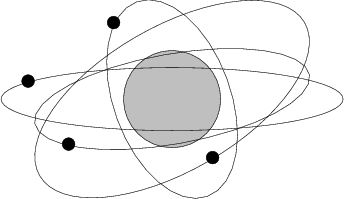
\epsfig{file={../fig/atome},width=6 cm,angle=-90}}   
 \caption{Mod\`ele plan\'etaire de l'atome : des \'electrons gravitent
autour d'un noyau. Cette description de l'atome est d\'esormais
remplac\'ee par une description probabiliste dans le cadre de la
m\'ecanique quantique.}
 \label{figatome}
\end{figure}

\section{Les mol\'ecules}
%%%%%%%%%%%%%%%%%%%%%%%%%
Une mol\'ecule\cite{ph:mecaq:Cohen73,ph:mecaq:Rivail89} est un
arrangement de quelques atomes \index{mol\'ecule}(de deux \`a 
quelques centaines). Les propri\'et\'es des mol\'ecules peuvent
\^etre bien d\'ecrites par la m\'ecanique quantique (voir la section
\ref{secmolecmq}). La g\'eom\'etrie d'une
mol\'ecule suffit parfois \`a comprendre ses propri\'et\'es. La
figure \ref{figc60fig} repr\'esente une mol\'ecule de Fuller\`ene C60,
\`a l'origine du prix Nobel 1996 de chimie des Profs Curl, Kroto, et Smalley.
\begin{figure}[htb]
 \centerline{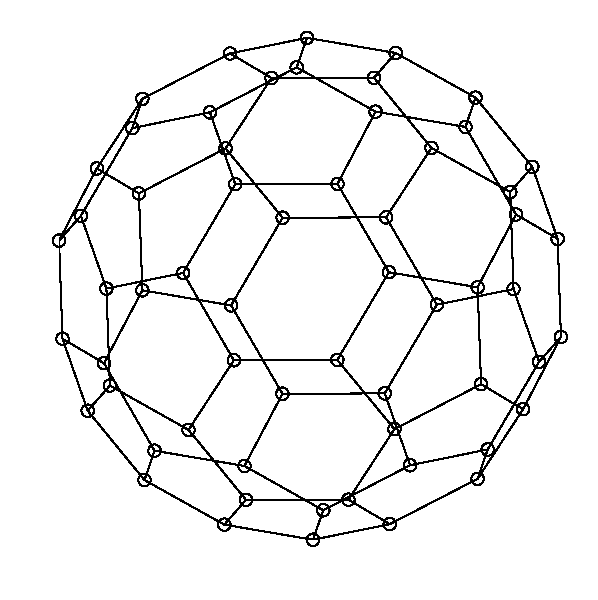
\epsfig{file={../fig/c60fig},width=6 cm}}   
 \caption{La mol\'ecule de fuller\`ene C60 (ou football\`ene) est un
exemple de mol\'ecule g\'eante que sa taille tend \`a  rapprocher de
l'\'etat cristallin.} 
 \label{figc60fig}
\end{figure}
L'existence d'une telle mol\'ecule avait \'et\'ee intuit\'ee par
l'\'etude du spectre d'absorption de certaines \'etoiles lointaines.
Curl, Kroto, et Smalley ont r\'eussi \`a la fabriquer sur terre.
La mol\'ecule C60 est compos\'ee de 12 pentagones et 20 hexagones.
C'est la plus petite structure sph\'erique que l'on puisse construire
avec des polygones.\index{fuller\`ene}
Pour l'\'etude des mol\'ecules particuli\`eres que sont les
polym\`eres, nous renvoyons \`a \cite{ph:ploym:Doi96}.
\section{Les solides cristallins}
%%%%%%%%%%%%%%%%%%%%%%%%%%%%%%%%
Les solides cristallins \cite{ph:solid:Kittel67,ph:solid:Ashcroft76}
sont un arrangement p\'eriodique d'atomes ou de 
mol\'ecules. \index{cristal}Les sym\'etries de translation permettent de calculer des
approximations des \'etats quantiques de tels syst\`emes (voir la section
\ref{secsolidmq}). La physique
statistique permet d'\'evaluer leurs propri\'et\'es \`a l'\'equilibre (section
\ref{secgazparfq}).
L'approximation continue permet de mener des calculs de dynamique comme
par exemple en \'elasticit\'e(voir les sections \ref{sepripuiva} et
\ref{secmaterelast}).  
Parmi les propri\'et\'es des solides, introduisons ici les
propi\'et\'es magn\'etiques des solides.
Supposons que le constituant \'el\'ementaire du solide (par exemple
une petite mol\'ecule) pr\'esente un petit moment magn\'etique\index{moment magn\'etique} ou spin. Si
l'orientation de ces spins est al\'eatoire on dit que le cristal est
paramagn\'etique\index{paramagn\'etique} (voir figure\ref{figparamag}). 
\begin{figure}[htb]
 \centerline{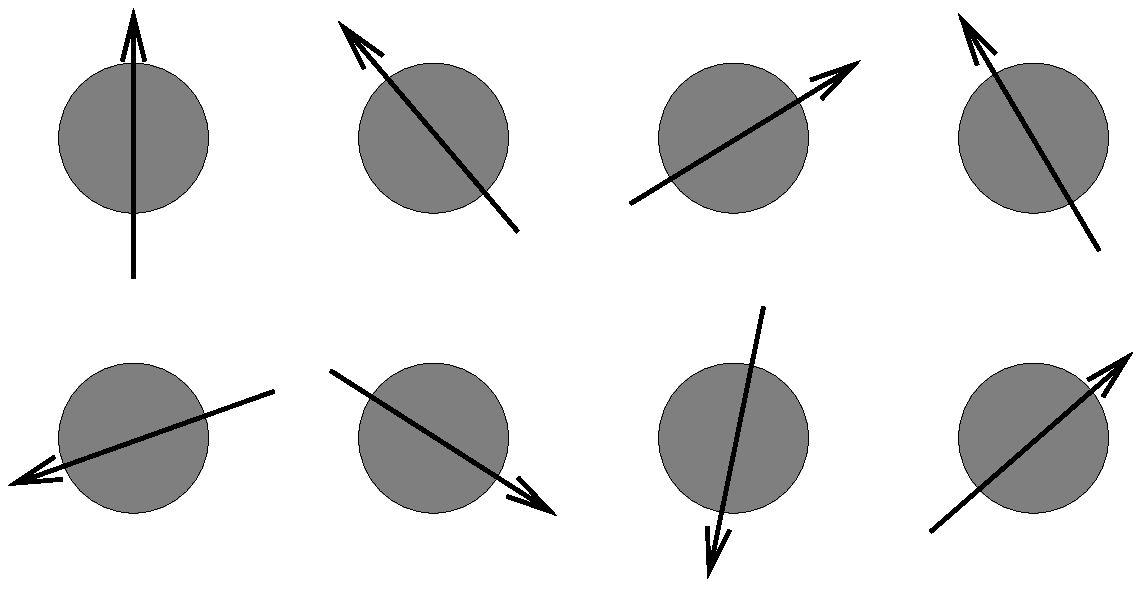
\epsfig{file={../fig/paramag},width=6 cm,angle=-90}}   
 \caption{Dans un solide paramagn\'etique, les spins sont orient\'es
au hasard, l'aimentation totale est donc nulle.}
 \label{figparamag}
\end{figure}
L'aimentation est alors
nulle en moyenne. Si les spins sont orient\'es selon une direction
privil\'egi\'ee on dit que le cristal est ferromagn\'etique\index{ferromagn\'etique}  (voir
figure\ref{figferromag}). 
L'aimentation est alors non nulle.
\begin{figure}[htb]
 \centerline{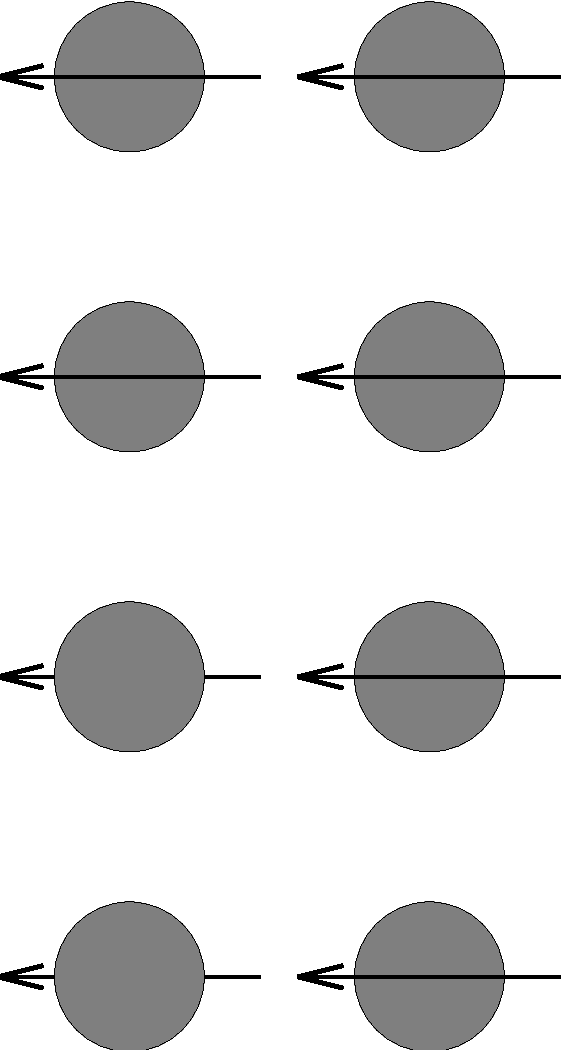
\epsfig{file={../fig/ferromag},width=6 cm,angle=-90}}   
 \caption{Dans un cristal f\'erromagn\'etique, les spins sont
orient\'es suivant une direction privil\'egi\'ee.}
 \label{figferromag}
\end{figure}
Si les spins poss\`edent une orientation alternativement oppos\'ee
(voir figure \ref{figantiferromag}), on parle d'antif\'erromagn\'etisme.
\begin{figure}[htb]
 \centerline{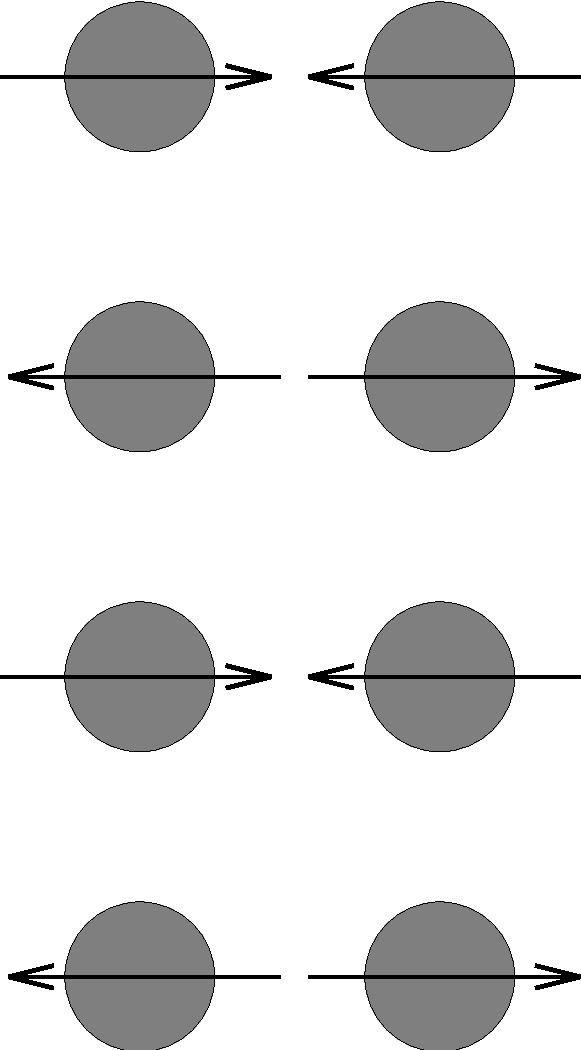
\epsfig{file={../fig/antiferromag},width=6 cm,angle=-90}}   
 \caption{Dans un cristal antif\'erromagn\'etique, deux spins voisins sont
orient\'es suivant des directions oppos\'ees.}
 \label{figantiferromag}
\end{figure}
Le mod\`ele d'Ising (voir la section \ref{secmodising}) est un mod\`ele simple
qui permet de d\'ecrire la 
{\bf transition paramagn\'etique -- f\'erromagn\'etique} qui appara\^\i t
pour certains mat\'eriaux (par exemple le fer) lorsque la temp\'erature baisse.

\section{Les gaz et liquides}
%%%%%%%%%%%%%%%%%%%%%%%%%%%%%%
Les gaz\index{gaz} et les liquides\cite{ph:physt:Diu89} correspondent \`a une r\'epartition
al\'eatoire de constituants \'el\'ementaires (atomes ou mol\'ecules).
Les particules d'un gaz sont caract\'eris\'ees par une \'energie
cin\'etique grande par rapport \`a l'\'energie typique d'interaction
entre les mol\'ecules. Lorsque l'\'energie cin\'etique des particules
devient du m\^eme ordre que l'\'energie d'interaction entre les
particules, le gaz se transforme en liquide.
Le mod\`ele de Van der Walls permet de d\'ecrire la {\bf transition liquide
-- vapeur} (voir la section \ref{secvanderwaals}).
\section{Autres arrangements de mati\`ere}
%%%%%%%%%%%%%%%%%%%%%%%%%%%%%%%%%%%%%%%%%%
\subsection{Quasicristaux}
%%%%%%%%%%%%%%%%%%%%%%%%%%
Les quasicristaux\cite{ph:quasi:Pignon94,ph:quasi:Jaric88}
d\'ecouverts par le physicien isra\'elien Shechtman 
en 1982 correspondent \`a un remplissage non p\'eriodique d'un volume
par des atomes ou mol\'ecules. Le pentagone est une forme interdite en
cristallographie : on ne peut remplir un volume avec des celules
\'el\'ementaires de sym\'etrie d'ordre cinq r\'eparties
p\'eriodiquement. Ce probl\`eme \`a trois dimensions est analogue au
probl\`eme du pavage du plan. On ne peut couvrir un sol avec seulement
des pentagones.
Le math\'ematicien anglais Penrose \index{Penrose}a d\'ecouvert des pavages
non p\'eriodiques 
du plan en formant des d\'ecagones \`a partir de losanges de deux
types (voir figures \ref{figpenrose} et \ref{figpenrose2}). 
\begin{figure}[htb]
 \centerline{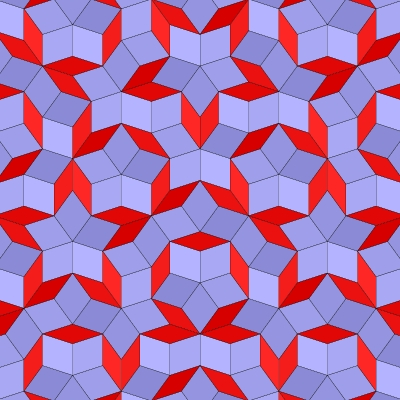
\epsfig{file={../fig/penrose},width=6 cm,angle=-90}}   
 \caption{Pavage de Penrose : \`a partir de deux types de losanges, on
peut construire un pavage non p\'eriodique du plan.}
 \label{figpenrose}
\end{figure}
\begin{figure}[htb]
 \centerline{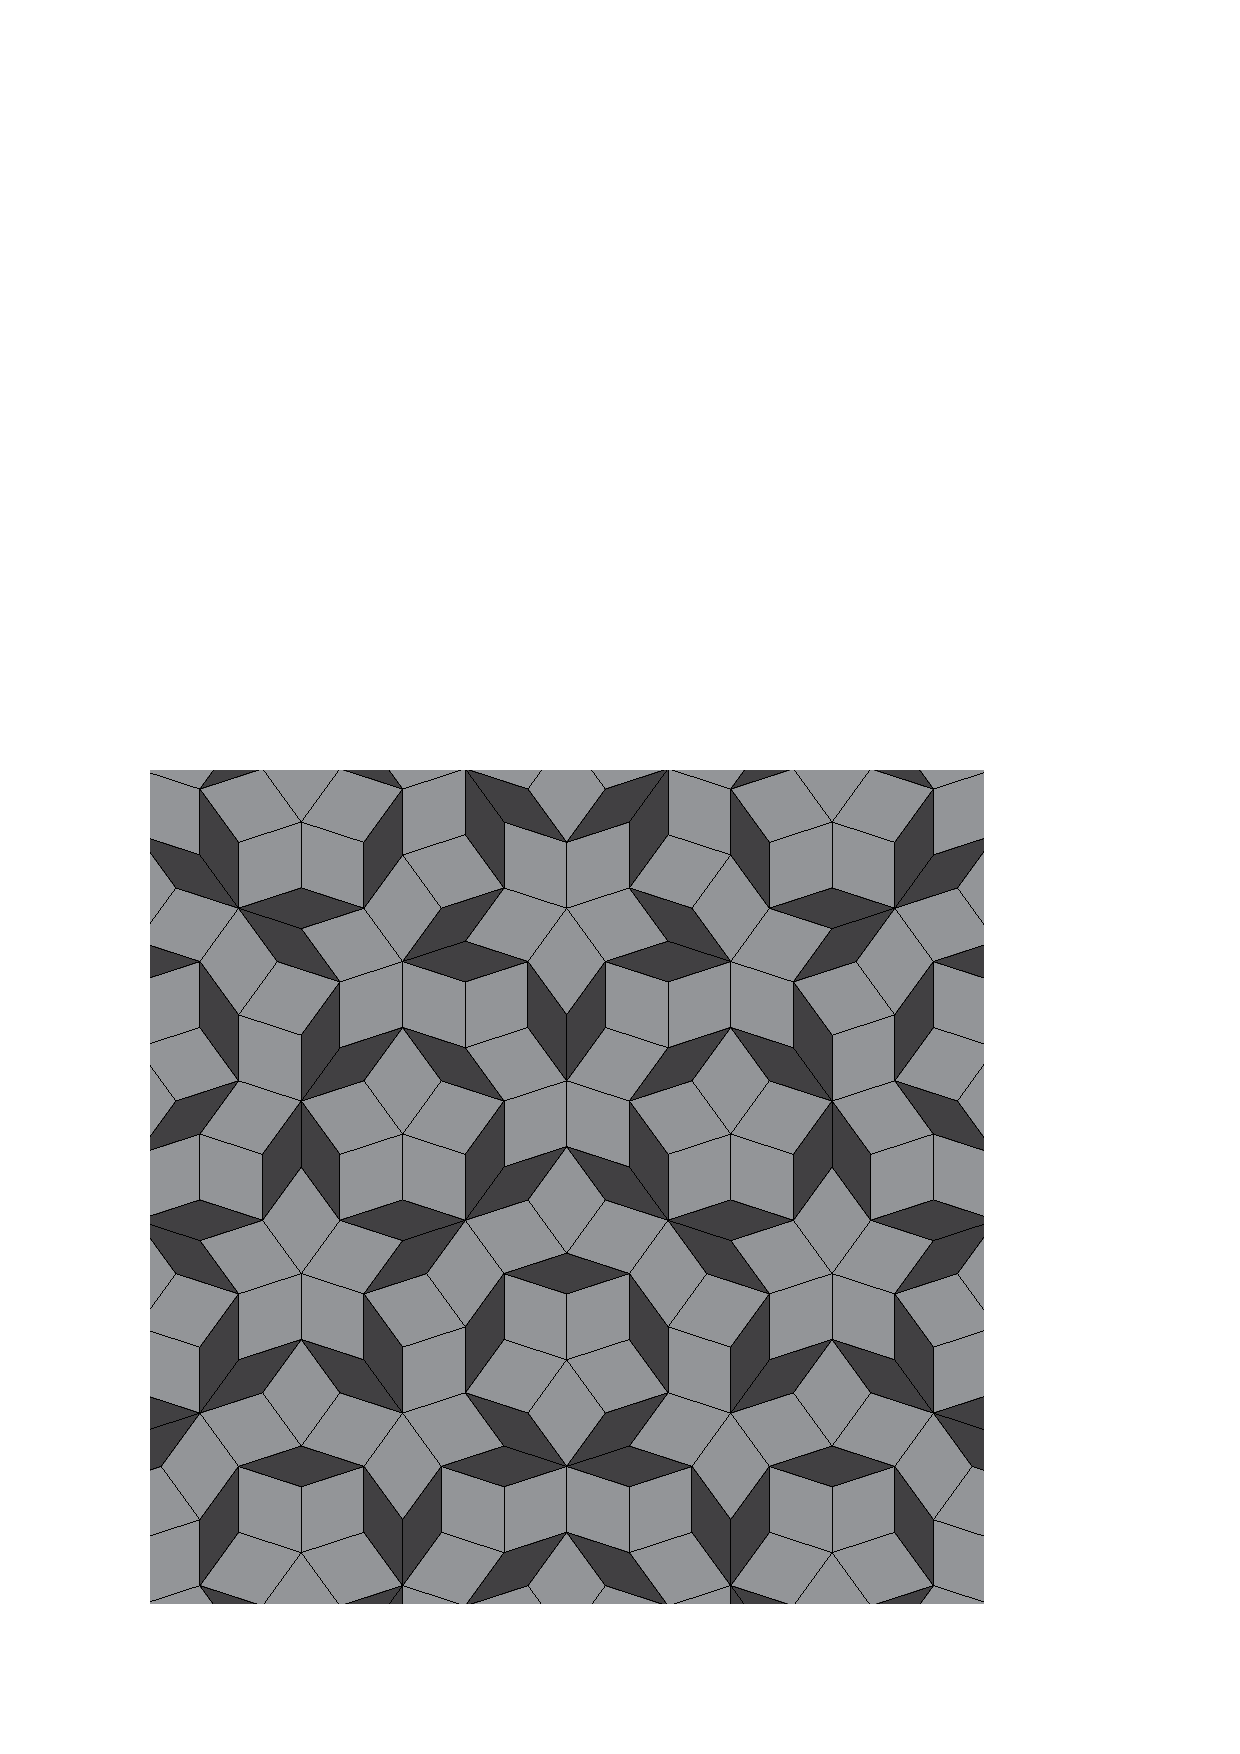
\epsfig{file={../fig/penrose2},width=6 cm,angle=-90}}   
 \caption{Pavage de Penrose : m\^eme figure que la pr\'ec\'edente avec
deux couleurs seulement, pour distinguer les deux types de losanges
\'el\'ementaires. }
 \label{figpenrose2}
\end{figure}
Les
structures obtenues sont \'etonamment complexes et il est impossible
de trouver un motif qui se r\'ep\`ete quel que soit l'ensemble de
losanges consid\'er\'e.  
\subsection{Cristaux liquides}\label{secristliquides}
%%%%%%%%%%%%%%%%%%%%%%%%%%%%%%
Les cristaux liquides \cite{ph:liqcr:Veyssie94,ph:liqcr:DeGennes74}
qui portent aussi le nom de phases m\'esomorphes 
sont des \'etats interm\'ediaires entre l'ordre parfait du cristal et
le d\'esordre du liquide. Les mol\'ecules qui composent les cristaux
liquides\index{cristal liquide} ont la forme allong\'ee d'un cigare. Ces mol\'ecules
s'organisent dans l'espace de fa\c con \`a r\'ealiser une \'etat
``fluide'' plus ou moins ordonn\'e. Parmis les cristaux liquides, ont
distingue plusieurs phases.  Dans la phase {\bf n\'ematique}\index{n\'ematique} (voir figure
\ref{fignematique}) les axes des mol\'ecules restent parall\`eles
entre eux. D\`es lors, il existe une direction privil\'egi\'ee de
l'espace. Ces mol\'ecules peuvent se d\'eplacer les unes par rapport
aux autres, mais comme les poissons d'un ban de poissons, elle garde
une direction privil\'egi\'ee.
\begin{figure}[htb]
 \centerline{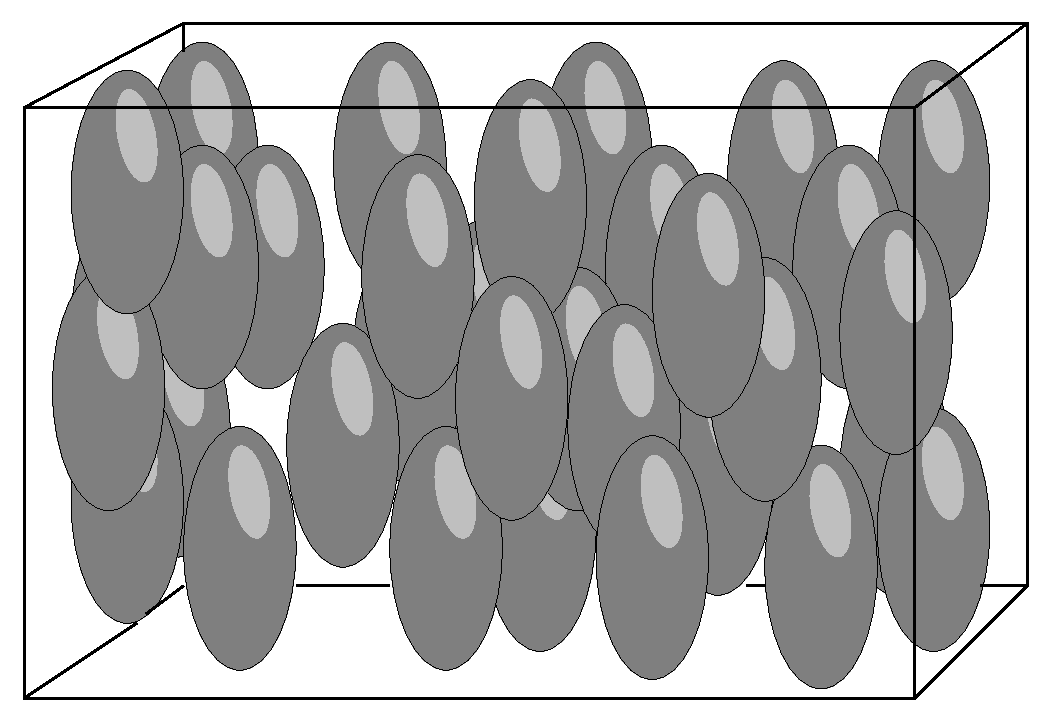
\epsfig{file={../fig/nematique},width=6 cm,angle=-90}}   
 \caption{Un mat\'eriau n\'ematique est l'analogue du banc de
poissons. Les mol\'ecules sont orient\'ees suivant une direction
privil\'egi\'ee mais sont en des positions al\'eatoires.}
 \label{fignematique}
\end{figure}
Quand les mol\'ecules constitutives ne sont pas superposables \`a leur
propre image dans un miroir, il apparait une torsion de la structure
n\'ematique : on appelle cette phase la phase
{\bf cholest\'erique}\index{cholesterique}  (voir
figure~\ref{figcholesteric}).
\begin{figure}[htb]
 \centerline{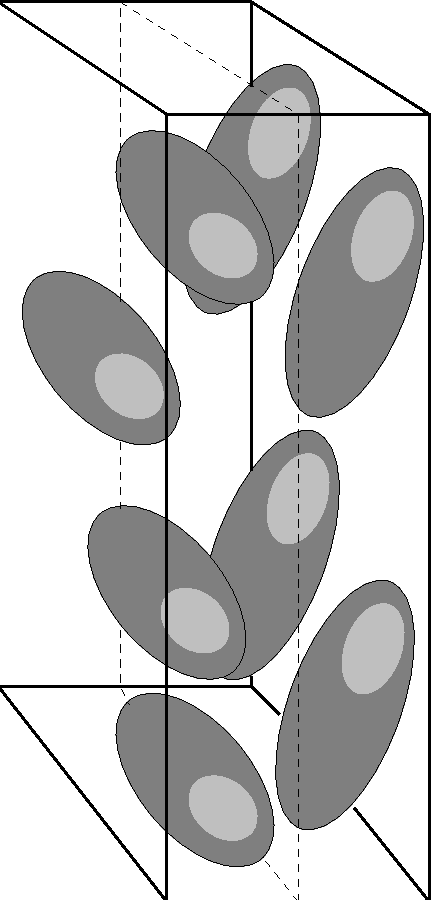
\epsfig{file={../fig/cholesteric},width=6 cm,angle=-90}}   
 \caption{Dans un mat\'eriau cholest\'erique, les mol\'ecules se
disposent en couches. Dans chaque couche, les mol\'ecules s'orientent
suivant une direction privil\'egi\'ee. Cette direction varie
r\'eguli\`erement d'une couche \`a l'autre pour former une structure
en h\'elice.}
 \label{figcholesteric}
\end{figure}
Une structure plus ordonn\'ee est celle de la phase {\bf smectique}\index{smectique} : les
mol\'ecules sont rang\'ees dans des couches et ces couches se
superposent (voir figure\ref{figsmectiqueA}). Le caract\`ere fluide
vient du fait que les couches peuvent glisser l'une sur l'autre.
\begin{figure}[htb]
 \centerline{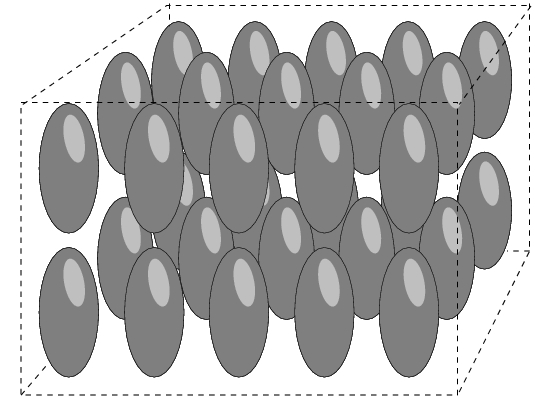
\epsfig{file={../fig/smectiqueA},width=6 cm,angle=-90}}   
 \caption{Smectique A}
 \label{figsmectiqueA}
\end{figure}
Pour d\'ecrire les d\'eformations des n\'ematiques, on utilise un
champ de vecteurs. Pour d\'ecrire les d\'eformations des smectiques, on
caract\'erise l'\'etat par une surface $u_i(x,y)$.
\`A la section \ref{secenernema}, nous \'etudierons les propri\'t\'es
\'energ\'etiques des mat\'eriaux n\'ematiques.
\subsection{Collo\"\i des}
%%%%%%%%%%%%%%%%%%%%%
Les collo\"\i des\index{collo\"\i de} sont des \'etats finement divis\'es et dispers\'es
de la mati\`ere. Des exemples sont les \'emulsions\index{\'emulsion} et a\'erosols.
Consid\'erons un syst\`eme compos\'e de mol\'ecules qui comporte deux
parties : une t\^ete polaire qui est soluble dans l'eau et une queue
hydrophobe qui est insoluble dans l'eau. De telles mol\'ecules sont
appel\'ees amphiphiles. De telle mol\'ecules plong\'ees dans l'eau
vont s'assembler en des structures appel\'ees micelles\index{micelle} (voir figure
\ref{fighuileeau}). Les mol\'ecules tournent leur t\^ete vers l'eau et
leur queue vers l'int\'erieur de la structure.
\begin{rem}
Les cellules du monde vivant sont tr\`es proches des micelles, et
c'est certainement par l'interm\'ediaire de telles structures qu'est
apparue la vie. 
\end{rem}

\begin{figure}[htb]
 \centerline{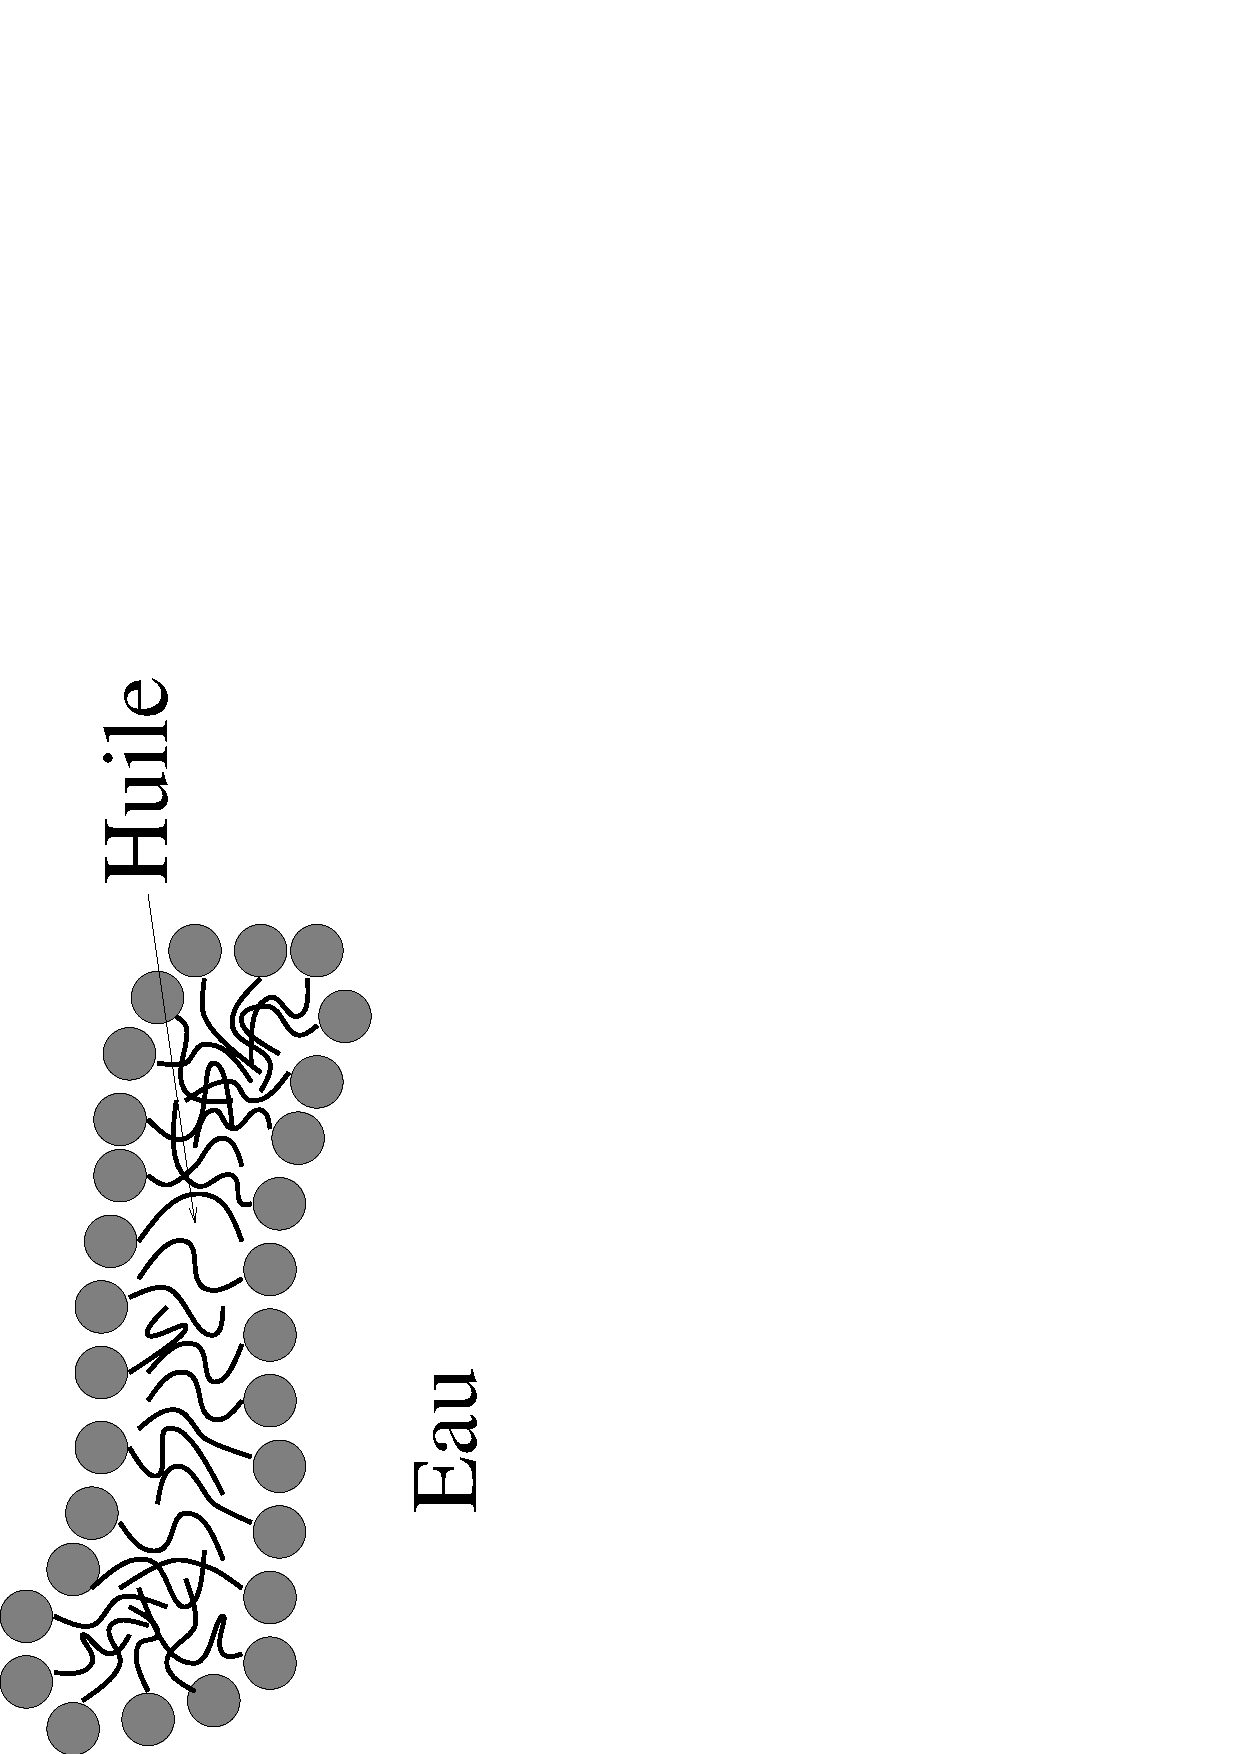
\epsfig{file={../fig/huileeau},width=6 cm,angle=-90}}   
 \caption{Des mol\'ecules amphiphile (comme celle de l'huile) qui
comportent une t\^ete hydrophile et une queue hydrophobe s'organisent
de mani\`ere \`a former des structures appel\'ees micelles.}
 \label{fighuileeau}
\end{figure}
On trouve ce genre de mol\'ecules dans la mayonnaise
\cite{ph:cooki:Grosser81,ph:cooki:McGee84,ph:cooki:McGee90,ph:cooki:This93}.
Des susbtances dites tensio-actives permettent de dissoudre des
micelles (application aux produits lessiviers).

Les mousses sont des arrangements de mol\'ecules similaires
\cite{ph:foams:Adamson76,ph:foams:Aubert86,ph:foams:Bikerman73}.


\subsection{Verre}
%%%%%%%%%%%%%%%%%%
L'\'etat vitreux\cite{ph:mater:Zallen83} est caract\'eris\'e par une
r\'epartition al\'eatoire des mol\'ecules dans le volume (voir figure
\ref{figglass}. Le verre\index{verre} est 
solide, ce qui implique que les mouvements des diff\'erents
constituants est faible.
\begin{figure}[htb]
 \centerline{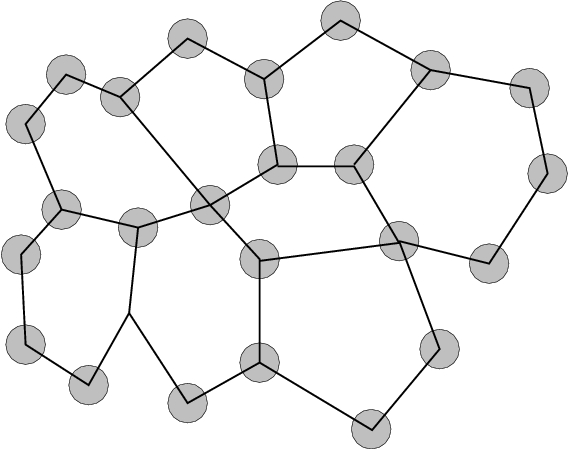
\epsfig{file={../fig/glass},width=6 cm,angle=-90}}   
 \caption{Le verre est caract\'eris\'e par une grande rigidit\'e comme
les cristaux, mais les positions des atomes sont al\'eatoires.}
 \label{figglass}
\end{figure}
La transition de phase de l'\'etat liquide \`a l'\'etat vitreux se fait
progressivement. 

Un mat\'eriau proche du verre peut etre r\'ealis\'e en compressant des
petites particules sph\'eriques. Sous les forces de pression, les
boules vont se d\'eformer et se coller entre elles. On peut alors se
poser la question : les interstices restant dans le mat\'eriau
vont-ils \^etre suffisamment nombreux pour laisser passer un liquide
par exemple. Ce probl\`eme est un cas particulier du ph\'enom\`ene\index{percolation} de
{\bf percolation}\cite{ph:mater:Zallen83}. La figure \ref{figpercol}
illustre ce ph\'enom\`ene dans une exp\'erience pr\'esent\'ee dans  \cite{ph:mater:Zallen83}.
\begin{figure}[htb]
 \centerline{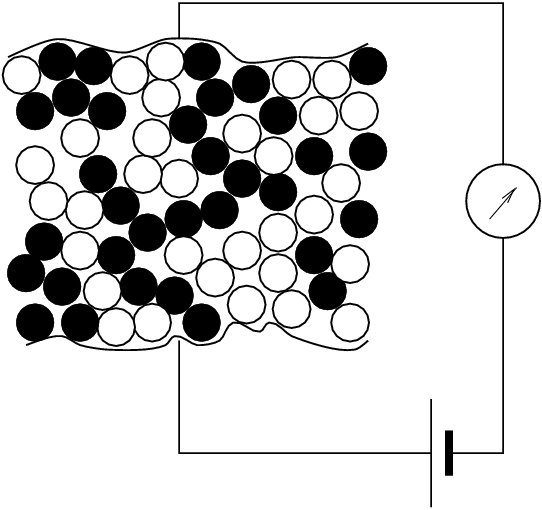
\epsfig{file={../fig/percol},width=6 cm,angle=-90}}   
 \caption{Exemple de percolation : les billes noires sont
conductrices, les billes blanches sont isolantes. On mesure le courant
parcourant le circuit en fonction de la proportion $p$ de billes
blanches. Il existe une proportion critique $p_c$ au dela de laquelle
plus aucun courant ne circule. L'\'etude du point critique permet de
montrer qu'il existe des propri\'et\'es universelles recontr\'ees dans
tous les syt\`emes similaires.} 
 \label{figpercol}
\end{figure}
Un autre exemple plus simple est celui de la grille
vandalis\'ee\cite{ph:mater:Zallen83} o\`u 
l'on d\'etruit les connections d'une maille conductrice avec la
probabilit\'e $p$.

Les verres de spin sont des mat\'eriaux magn\'etiques d\'esordonn\'es.
Un bon exemple de verre de spin est fourni par l'alliage cuivre
mangan\`ese, not\'e CuMn o\`u des atomes de mangan\`ese, porteurs de
moment magn\'etique sont dispers\'es au hasard dans une matrice de
cuivre. Deux spin ont tendance dans ce syst\`eme soit \`a s'aligner
dans le m\^eme sens, soit \`a s'aligner dans des sens oppos\'es selon
la distance qui les s\'epare (voir figure \ref{figspinglass}).
\begin{figure}[htb]
 \centerline{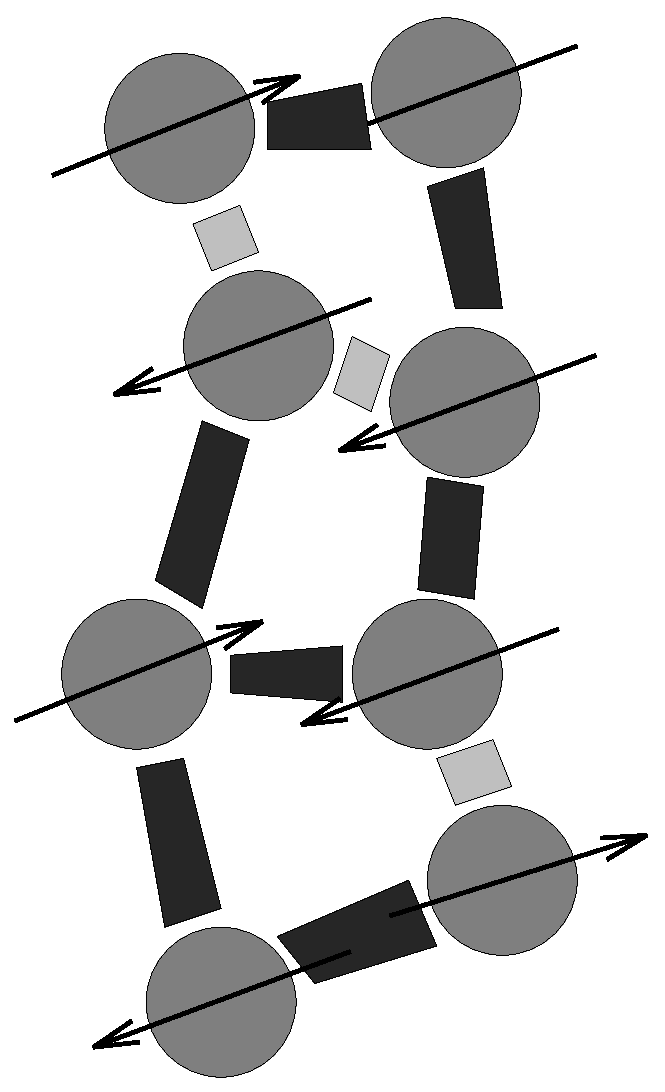
\epsfig{file={../fig/spinglass},width=6 cm,angle=-90}}   
 \caption{Dans un verre de spin les interactions entre spins voisins
sont al\'eatoirement de type ferromagn\'etique ou
antiferromagn\'etique, du fait de la position al\'eatoire des spins.}
 \label{figspinglass}
\end{figure}
On obtient donc un syst\`eme frustr\'e : il n'existe pas de
configuration pour laquelle toutes les \'energies d'interaction entre
voisins sont minimales. L'exemple le plus simple de syst\`eme
frustr\'e est donn\'e par un syst\`eme constitu\'e de trois spins
1,2,3. Si les r\`egles d'interaction sont les suivantes: l'\'energie
d\'ecroit si 1 et 2 sont de m\^eme sens, 2 et 3, de m\^eme sens et 1
et 3 de sens oppos\'e. Les verres de spins seront abord\'es \`a la section
\ref{secverredespi}.


\subsection{Tas de sable, tas d'oranges}
%%%%%%%%%%%%%%%%%%%%%%%%%%%%%%%%%%%%%%%
Les syst\`emes physiques granulaires suscitent de nombreuses recherches
\`a l'heure actuelle. Ces syst\`emes exhibent \`a la fois des
propri\'et\'es de solide et de liquide. C'est le cas du tas de sable.
Ainsi le
sable qui s'\'ecoule dans un sablier ne s'\'ecoule pas de la m\^eme
mani\`ere qu'un liquide : la vitesse d'\'ecoulement ne d\'epend pas de
la quantit\'e de sable dans le compartiment du dessus. La formation
du tas de sable du bas se fait par convection interne des grains
compens\'ee par un ph\'enom\`ene d'avalanche\index{avalanche} \`a la surface du tas.
Nous renvoyons pour ce sujet aux r\'ef\'erences \cite{ph:granu:Guyon94}. On y
traite, en particulier du ph\'enom\`eme d'avalanche et d\'ecoulement. 


\chapter{Relativit\'e}\label{chaprelat}
%%%%%%%%%%%%%%%%
\section{Introduction}
%%%%%%%%%%%%%%%%%%%%%%
Dans ce chapitre nous pr\'esentons diff\'erentes mani\`eres de g\'eom\'etriser
l'espace physique. Une lecture pr\'ealable des annexes sur les tenseurs et sur
les d\'eriv\'ees (covariantes) pourra \^etre utile au lecteur peu familier
avec ces notions.
il existe plusieurs formalismes possibles pour d\'ecrire les syst\`emes
physiques. Nous envisageons dans ce chapitre les formalismes associ\'es \`a la
description d'un point mat\'eriel.
En m\'ecanique classique, un point mat\'eriel de masse $m$ est rep\'er\'e par
sa position $r$ et son impulsion $p$ \`a l'instant $t$. Le temps ne d\'epend
pas du r\'ef\'erentiel dans lequel on \'evalue la position et l'impulsion de
la particule. En relativit\'e
restreinte et g\'en\'erale, le temps d\'epend du r\'eferentiel consid\'er\'e
ce qui entraine \`a modifier la notion classique de position et d'impulsion.
Nous reportons aux chapitres suivant la description quantique, cin\'etique et
continue de la mati\`ere\footnote{%%%%%%%%%%%%%%%%%%%%%%%%%%%%%%%%
En m\'ecanique quantique, l'espace physique consid\'er\'e est un espace
fonctionnel, et un 
syst\`eme est repr\'esent\'e par une fonction d'onde $\phi(r,t)$ de l'espace
et du 
temps. La quantit\'e $\phi(r,t)dr$  s'interpr\`ete comme la
probabilit\'e d'avoir \`a l'instant $t$ une particule dans le volume
$dr$.
La fonction d'onde se g\'en\'eralise \`a des syst\`emes plus complexes
que ceux constitu\'es d'une particule.
Une description cin\'etique d'un syst\`eme consitu\'e d'un grand nombre de
particule consiste \`a repr\'esenter l'\'etat du syst\`eme par une fonction
dite de r\'epartition $f(r,p,t)$ qui repr\'esente la densit\'e de
probabilit\'e de trouver une particule en $r$ avec une impulsion $p$.
La description continue de la mati\`ere fait appel \`a plusieurs fonctions de
la position et du temps pour d\'ecrire le syst\`eme physique.}.%%%%%%%%%%%%

Nous introduisons ensuite les premi\`eres lois de la dynamique : dynamique du
point classique, dynamique du point en relativit\'e restreinte et
g\'en\'eralis\'ee.  L'\'equation
de Schr\"odinger qui d\'ecrit la dynamique d'un syst\`eme quantique sera
introduite au chapitre \ref{chapmq}. Les \'equations de la dynamique pour une
description cin\'etique d'un grand nombre de particules font l'objet de la
section \ref{desccinet}. La 
dynamique des milieux continus sera 
\'etudi\'ee au chapitre \ref{chapapproxconti}.


\section{G\'eom\'etrisation de l'espace}
%%%%%%%%%%%%%%%%%%%%%%%%%%%
\subsection{M\'ecanique classique}
%%%%%%%%%%%%%%%%%
La m\'ecanique classique est fond\'ee sur deux principes fondamentaux
: le principe de {\bf relativit\'e de Galil\'ee}\index{Galil\'ee
(relativit\'e de)} et le principe fondamental
de la dynamique.
\'Enon\c cons le principe de relativit\'e de Galil\'ee :
\begin{prin}
{\bf Principe de Relativit\'e de Galil\'ee.}
Les lois de la m\'ecanique classique (en particulier la relation
fondamentale de la dynamique) sont les m\^emes dans tous les
r\'ef\'erentiels anim\'es les uns par rapport aux autres d'un mouvement de
translation uniforme. De tels syst\`emes sont appel\'es r\'ef\'erentiels
Galil\'eens (ou d'inertie)
\end{prin}
\begin{rem} Les lois sont invariantes par des transformations
appartenant au groupe de transformation de Galil\'ee. Elle s'\'ecrivent :
\begin{eqnarray}
x'_1&=&x_1-vt\\
x'_1&=&x_1\\
x'_1&=&x_1\\
t'&=&t
\end{eqnarray}
\end{rem}

\subsection{M\'ecanique relativiste (Relativit\'e
restreinte)}\label{secrelat} 
%%%%%%%%%%%%%%%%%%%%%%%%%%
La m\'ecanique relativiste introduite par Einstein dans le cadre
restreint est bas\'ee sur plusieurs postulats.
\begin{postulat}
Les lois de la m\'ecanique et de l'\'electromagn\'etisme (c'est
\`a dire 
toutes les lois de l'univers) sont les m\^emes dans tous les
r\'ef\'erentiels Galil\'eens.
\end{postulat}
\begin{postulat}
La vitesse de la lumi\`ere dans le vide $c$ est la m\^eme dans tous
les r\'ef\'erentiels Galil\'eens. Cette vitesse constitue une limite
sup\'erieure
\end{postulat}

L'existence d'une vitesse universelle, la vitesse de la lumi\`ere, va
profond\'ement modifier la structure de l'espace--temps
\index{espace--temps}. Elle nous conduit \`a
pr\'eciser la m\'etrique\index{m\'etrique} que l'on adopte en relativit\'e restreinte.
Consid\'erons deux syst\`emes Galil\'eens caract\'eris\'es par les
coordonn\'ees 
$(x,t)$ et  $(x^\prime,t^\prime)$. Supposons qu'a $t=t^\prime=0$ les
deux syst\`emes co\"\i ncident. Alors :
\begin{equation}
c=\frac{|x|}{|t|}=\frac{|x^\prime|}{|t^\prime|}
\end{equation}
ce qui revient \`a dire :
\begin{equation}
c^2t^2-x^2=0
\end{equation}
et
\begin{equation}
c^2t^{\prime 2}-x^{\prime 2}=0
\end{equation}
La quantit\'e $c^2t^2-x^2$ est donc un invariant.
La m\'etrique la plus naturelle avec laquelle il convient de munir
l'espace temps est donc :
\begin{equation}
ds^2=dx^2+dy^2+dz^2-c^2dt^2
\end{equation}
Nous postulons que cette m\'etrique doit \^etre invariante par un
changement de coordonn\'ees galil\'een.
\begin{postulat}
La m\'etrique $ds^2=dx^2+dy^2+dz^2-c^2dt^2$ est invariante par
changement de r\'ef\'erentiel Galil\'een.
\end{postulat}

Cherchons maintenant la repr\'esentation d'une transformation de
l'espace--temps qui laisse invariante cette m\'etrique.
Nous cherchons les transformations telles que :\index{Lorentz
(transformation de)}
\begin{equation}
ds^2=dx^2+dy^2+dz^2-c^2dt^2
\end{equation}
soit invariant.
Nous devons d'abord d\'efinir ce que nous appelons le vecteur position
dans l'espace--temps (ou quadri--vecteur position)\index{quadri--vecteur}.
Pour cela il y a deux formalismes possibles :
\begin{itemize}
\item Soit on prend comme composantes du quadri-vecteur position
$R=(x,y,z,ct)$ et on munit l'espace des quadri-vecteurs du pseudo-produit scalaire
de matrice :
\begin{equation}
D=
\left( \begin{array}{cccc}
1&0&0&0 \cr
0&1&0&0\cr
0&0&1&0\cr
0&0&0&-1\cr
\end{array} \right)
\end{equation}
Alors :
\begin{equation}
(R|R)=R^tDR
\end{equation}
o\`u $R^t$ d\'esigne le transpos\'e du quadri-vecteur position $R$.
\item Soit on prend comme composantes du quadri-vecteur position
$R=(x,y,z,ict)$ et on munit l'espace des quadri-vecteurs du pseudo-produit scalaire
de matrice :
\begin{equation}
D=Id=
\left( \begin{array}{cccc}
1&0&0&0 \cr
0&1&0&0\cr
0&0&1&0\cr
0&0&0&1\cr
    \end{array} \right)      
\end{equation}
Alors :
\begin{equation}
(R|R)=R^tR
\end{equation}
o\`u $R^t$ d\'esigne le transpos\'e du quadri-vecteur position $R$.
\end{itemize}
Une fois le formalisme choisi, nous pouvons trouver la forme des
matrices qui laisse la pseudo--norme invariante. (cf \cite{ph:relat:Hakim94}
p48) Ici 
nous nous contentons d'exhiber de telles matrices.
Dans le premier cas la condition que le pseudo-produit scalaire de
deux quadri-vecteurs soit invariant implique :
\begin{equation}
(MR|MR)=(R|R)
\end{equation}
donc
\begin{equation}
D=M^+DM
\label{cond}
\end{equation}
La matrice suivante convient :
\begin{equation}
M=
\left( \begin{array}{cccc}
\gamma&0&0&\gamma \beta \cr
0&1&0&0\cr
0&0&1&0\cr
\gamma \beta&0&0&\gamma\cr
         \end{array} \right)
\end{equation}
Son inverse est :
\begin{equation}
M^{-1}=
\left( \begin{array}{cccc}
\gamma&0&0&-\gamma \beta \cr
0&1&0&0\cr
0&0&1&0\cr
-\gamma \beta&0&0&\gamma\cr
          \end{array} \right)
\end{equation}
\begin{rem}
L'\'equation \ref{cond} implique une condition sur le d\'eterminant :
\begin{equation}
1=det(M^+DM)=(det(M))^2
\end{equation}
Les matrices $M$ de d\'eterminant 1 forment un groupe appel\'e groupe de
Lorentz.\index{Lorentz (groupe de)}
 \end{rem}
Dans le second cas cette m\^eme condition implique :
\begin{equation}
Id=M^+M
\end{equation}
La matrice suivante convient :
\begin{equation}
M=
\left( \begin{array}{cccc}
\gamma&0&0&-i\gamma \beta \cr
0&1&0&0\cr
0&0&1&0\cr
+i\gamma \beta&0&0&\gamma\cr
          \end{array} \right)
\end{equation}
et l'inverse :
\begin{equation}
M^{-1}=
\left( \begin{array}{cccc}
\gamma&0&0&+i\gamma \beta \cr
0&1&0&0\cr
0&0&1&0\cr
-i\gamma \beta&0&0&\gamma\cr
\end{array} \right)          
\end{equation}
\begin{rem}
On appelle matrice unitaire (voir la section \ref{secautresrep}) une
matrice telle que : 
\begin{equation}
M^+M=1=MM^+
\end{equation}
o\`u $M^+$ d\'esigne la matrice adjointe de $M$ c'est \`a dire la
transpos\'ee conjugu\'ee de $M$. Alors le produit scalaire d\'efini par :
\begin{equation}
 \langle R|Q\rangle =R^+Q
\end{equation}
est conserve sous l'action de $M$.
\end{rem}

\subsubsection{Temps propre}
Le quadri-scalaire (ou invariant de Lorentz) $d\tau$ va nous
permettre de d\'efinir d'autres quadri-vecteurs (comme la vitesse):
\begin{defn}
Le temps propre d'un mobile est le temps marqu\'e par une horloge
invariablement li\'e \`a ce mobile.  
\end{defn}
Si le mobile se d\'eplace \`a la vitesse $v$ dans $R_2$ alors les \'ev\`enements A et B qui
ont pour coordonn\'ees dans le r\'ef\'erentiel $R_1$ li\'e au mobile :
\begin{eqnarray}
x_A=0& &x_B=0\\
ct_A=0& &ct_B=c\tau
\end{eqnarray}
ont pour coordonn\'ees dans le r\'ef\'erentiel $R_2$
\begin{eqnarray}
x_A=0& &x_B=vt\\
ct_A=0& &ct_B=ct
\end{eqnarray}
D'o\`u
\begin{equation}
\tau^2=-t^2(1-\frac{v^2}{c^2})
\end{equation}
\subsubsection{Quadri-vecteur vitesse}
%%%%%%%%%%%%%%%%%%%%%%%%
Le  quadri-vecteur vitesse est d\'efini par :
\begin{equation}
U=\frac{dX}{d\tau}
\end{equation}
\subsubsection{Autres quadri-vecteurs}
%%%%%%%%%%%%%%%%%%%%%%%%
Donnons quelques quadri-vecteurs dans le premier formalisme :
\begin{itemize}
\item quadri-vecteur position :
\begin{equation}
X=(x_1,x_2,x_3,ct)
\end{equation}
\item quadri-vecteur onde :
\begin{equation}
K=(k_1,k_2,k_3,\frac{\omega}{c})
\end{equation}
\item quadri-vecteur nabla :
\begin{equation}
K=(\frac{\partial}{\partial x_1},\frac{\partial}{\partial x_2},\frac{\partial}{\partial x_3},\frac{\partial}{\partial x_4})
\end{equation}
\end{itemize}


\subsection{Relativit\'e G\'en\'erale}
%%%%%%%%%%%%%%%%%%%%%%%%%%%%
Il existe deux m\'ethodes pour s'attaquer au probl\`eme de la d\'ecouverte
des lois de la nature (voir \cite{ph:relat:Charon63} p158):
\begin{enumerate}
\item La premi\`ere m\'ethode est celle que l'on peut qualifier de {\it
ph\'enom\'enologique}. Un bon exemple de th\'eorie
ph\'enom\'enologique est la 
m\'ecanique quantique. elle consiste \`a partir des faits connus par
l'exp\'erience et de chercher ensuite \`a inf\'erer les lois. On met au
centre de la th\'eorie la notion d'observable.
\item Il existe une autre m\'ethode moins ``anthropocentrique'' et dont
les avantages avaient \'et\'e soulign\'es au $17^{\grave eme}$ si\`ecle
par Descartes. 
C'est la m\'ethode {\it a priori} utilis\'ee par Einstein. Elle
consiste \`a partir de principes auxquels on croit et \`a chercher les
lois obe\"\i ssant \`a ces principes.
Voici sous forme de postulats les principes fondamentaux de la
relativit\'e g\'en\'erale :
\end{enumerate}
\begin{postulat}
{\bf Principe g\'en\'eralis\'e de relativit\'e}\cite{ph:relat:Charon63} :
Toutes les lois de la Nature sont covariantes \index{covariance}relativement \`a des
transformations continues quelconques des coordonn\'ees
\footnote{la relativit\'e restreinte affirme la covariance relativement
a la transformation de Lorentz cf \cite{ph:relat:Boudenot89} p53}
\end{postulat}
\begin{postulat}
{\bf Principe de simplicit\'e logique aussi grande que possible de la
formulation des lois :}
Toutes les caract\'eristiques {\bf g\'eom\'etriques} de
l'espace-temps  peuvent \^etre d\'ecrites au moyen d'un tenseur
diff\'erentiel $S$. Ce tenseur  
\begin{enumerate}
\item est exprim\'e dans un espace riemannien quadri-dimensionnel dont la
m\'etrique est d\'efinie par un tenseur $g_{ij}$
\item est du deuxi\`eme ordre, et est donc not\'e $S_{ij}$
\item est une fonction des $g_{ij}$ qui ne contient pas de
d\'eriv\'ees partielles d'ordre sup\'erieur \`a deux et qui est 
lin\'eaire par rapport aux d\'eriv\'ees partielles du deuxi\`eme ordre.
\end{enumerate}
\end{postulat}
\begin{postulat}
Troisi\`eme postulat :
La divergence des $S_{ij}$ est nulle.
\end{postulat}
\begin{postulat}
La courbure de l'espace est due \`a la mati\`ere:
\begin{equation}
{\rm Courbure}={\rm Mati\grave ere}
\end{equation}
soit :
\begin{equation}
S_{ij}=T_{ij}
\end{equation}
\end{postulat}
Einstein croit fermement en ces postulats. Par contre la mod\'elisation
du champ de gravitation peut \^etre am\'elior\'ee.
En partant de ces postulats, on peut d\'eduire l'\'equation d'Einstein.
Le seul tenseur $S_{ij}$ qui v\'erifie les postulats s\'ecrit :
\begin{equation}
S_{ij}=a(R_{ij}-\frac{1}{2}g_{ij}R-\lambda g_{ij})
\end{equation}
o\`u $a$ et $\lambda$ sont deux constantes et o\`u $R_{ij}$, le
tenseur de courbure de Ricci, et $R$ la courbure scalaire
sont des grandeurs d\'efinies \`a partir des $g_{ij}$ et qui ob\'eit
aux postulats.
Nous renvoyons aux ouvrages sp\'ecialis\'es pour l'expression de ces
grandeurs.
L'\'equation d'Einstein correspond au cas $a=1$. La constante
$\lambda$ est appel\'ee constante cosmologique.
Le tenseur de mati\`ere n'est pas d\'eduit de relation de sym\'etrie
comme le sont les termes $S_{ij}$. Einstein oppose ces deux termes en
disant que le terme de courbure est lisse comme l'or et le terme de
mati\`ere est rugueux comme le bois. Nous renvoyons \`a
\cite{ph:relat:Hakim94,ph:relat:Charon63} pour la mod\'elisation du tenseur de
mati\`ere.

\section{Dynamique}
%%%%%%%%%%%%%%
\subsection{Principe fondamental de la dynamique classique}
%%%%%%%%%%%%%%%%%%%%%%%%%%%%%%%
\'Enon\c cons le principe fondamental de la dynamique pour un
syst\`eme constitu\'e d'un point mat\'eriel. Nous verrons plus tard la
formulation adapt\'ee \`a la description des milieux continus. Un
point mat\'eriel est d\'ecrit par sa masse $m$ sa position $r$ et sa
vitesse $v$. Il subit des actions ext\'erieures mod\'elis\'ees par des
forces $F_{ext}$. On note $p$ la quantit\'e de mouvement $mv$
de la
particule (appel\'ee aussi impulsion de la particule) \index{impulsion}.
\begin{prin}
Le principe fondamental de la dynamique\index{principe fondamental de
la dynamique} affirme que la d\'eriv\'ee de
la quantit\'e de mouvement est \'egal \`a la somme des forces
ext\'erieures \index{force}:
\begin{equation}
\frac{dp}{dt}=\sum F_{ext}
\end{equation}
\end{prin}
\subsection{Principe de moindre action}\label{secprinmoindreact}
%%%%%%%%
\begin{prin}{\bf Principe de moindre action :}\index{principe de
moindre action} 
La fonction $x(t)$ d\'ecrivant la trajectoire d'une particule est
celle qui rend l'action stationnaire
\end{prin}
Ce principe peut servir de base \`a la fondation de la m\'ecanique du
point. Mais il peut aussi \^etre d\'eduit de la relation fondamentale
de la dynamique\cite{ma:equad:Arnold83}.
\begin{equation}
m \ddot{x}+\frac{\partial U}{\partial x}=0
\end{equation}
Multiplions par $y(t)$ et int\'egrons :
\begin{equation}
\int (m \ddot{x}y +\frac{\partial U}{\partial x}y)\,dt=0
\end{equation}
Utilisons le th\'eor\`eme de Green (int\'egration par parties)
\begin{equation}
\int (-m \dot{x}\dot{y} +\frac{\partial U}{\partial x}y)\,dt=0
\end{equation}
$\dot{x}\dot{y}$ est une forme bilin\'eaire.
\begin{equation}
-\dot{x}\dot{y}=-\frac{\partial }{\partial x}\frac{1}{2}\dot{x}^2
\end{equation}
\begin{equation}
0= \int m
[-\frac{1}{2}(\dot{x}\dot{y})^{2}+U(x+y)]-[-\frac{1}{2}\dot{x}^{2}+U(x)]dt+O(y^{2})
\end{equation}
\begin{equation}
0=-\delta \int L(\dot{x},x,t)dt
\end{equation}
\subsection{Description par les \'energies}
%%%%%%%%%%%%%%%%%%%%%%%%%%%%%%%%%%%%%%%%%%%
La relation fondamentale de la dynamique ne nous dit pas comment mod\'eliser
les forces. C'est au physicien de mod\'eliser les forces agissant sur la
particule. Donnons deux exemples de forces :
\begin{enumerate}
\item le poids $P=mg$. $g$ est une vecteur d\'ecrivant le champs
  gravitationnel dans le point o\`u se trouve la masse.
\item la force \'electromagn\'etique $f=qv\wedge B+qE$, o\`u $q$ est la charge
  de la particule, $E$ est le champ \'electrique, $B$ le champ magn\'etique et
  $v$ la vitesse de la particule.
\end{enumerate} 
Ces forces sont celles que l'on postule pour l'interaction gravitationnelle et
\'electromagn\'etique. Elles sont donc dans une certaine mesure fix\'ees.
Mais pour d'autres types de forces comme les forces \'elastiques, les forces
de frottement, la libert\'e laiss\'ee au mod\'elisateur est bien plus grande. 

Une m\'ethode efficace pour la mod\'elisation d'interactions complexes comme
celles ayant trait \`a l'elasticit\'e est d'utiliser le concept de puissance
(ou de travail). Au chapitre \ref{chapelectromag}, nous verrons l'\'equivalent
en terme de puissance de la force \'electromagn\'etique.
Aux chapitres \ref{chapapproxconti} et \ref{chapenermilcon} nous verrons
l'utilit\'e des concept de puissance et d'\'energie dans la mod\'elisation des
milieux continus. 

Rappelons ici les d\'efinitions associ\'ees \`a la description des interaction
par un vecteur force :
le travail \'el\'ementaire d'une force $f$ lors d'un d\'eplacement $dr$ est :
\begin{equation}
\delta W=f.dr
\end{equation}
La puissance instantan\'ee d\'egag\'e par une force appliqu\'ee \`a une masse
de vitesse $v$ est :
\begin{equation}
P=f.v
\end{equation}
L'\'energie potentielle gagn\'ee par la particule pendant le temps $dt$
qu'elle met pour 
se d\'eplacer de $dr$ est :
\begin{equation}
dE=-f.dr=-P.dt
\end{equation}
Il faut noter que l'\'energie potentielle ne peut \^etre d\'efinie que si le
champ de force $f$ est \`a circulation conservative. C'est le cas pour le
poids, pour la force \'electrique mais pas pour les forces de frottement.
Un syst\`eme qui subit de forces qui d\'erivent toutes d'un potentiel est dit
hamilonien. Les \'equations de la dynamique sont alors les {\'equations
  d'Hamilton} :
\begin{equation}\label{eqhampa1}
\frac{dp}{dt}=-\frac{\partial H}{\partial q}
\end{equation}
\begin{equation}\label{eqhampa2}
\frac{dq}{dt}=\frac{\partial H}{\partial p}
\end{equation}
o\`u la fonction $H(q,p,t)$ est appel\'ee hamilonien du syst\`eme.
Pour un syst\`eme d'une particule dans un potentiel $E_p$, le hamiltonien vaut
: 
\begin{equation}\label{eqformhami}
H(q,p,t)=\frac{p^2}{2m}+E_p(q)
\end{equation}
o\`u $p$ est l'impulsion de la particule et $q$ sa position.
Mais par extension, tout syst\`eme dont la dynamique est d\'ecrite par  les
\'equations \ref{eqhampa1} et \ref{eqhampa2} est appel\'e hamiltonien,\index{hamiltonien (syst\`eme)}
m\^eme si $H$ n'est pas de la forme \ref{eqformhami}.

\subsection{Dynamique en relativit\'e restreinte}
%%%%%%%%%%%%%%%%%%
Nous avons vu que les transformations de lorentz changent le temps.
Nous devons modifier les lois de la dynamique classique pour obtenir leur
invariance sous l'action du groupe de Lorentz. Le prix \`a payer est la
modification des notions d'impulsion et d'\'energie.
Nous imposons une d\'ependance lin\'eaire entre le quadri-vecteur
impulsion et le quadri-vecteur vitesse ;
\begin{equation}
P=mU=(m\alpha u,icm\alpha)
\end{equation}
o\`u $m$ est la masse au repos de la particule.
Appelons ''quantit\'e de mouvement relativiste'' la quantit\'e ;
\begin{equation}
p=m \alpha u
\end{equation}
et ''\'energie relativiste'' la quantit\'e :
\begin{equation}
E=m\alpha c^2
\end{equation}
Le quadri-vecteur $P$ s'\'ecrit donc aussi :
\begin{equation}
P=(p,i\frac{E}{c})
\end{equation}
Nous voyons qu'Einstein associe une \'energie \`a une masse puisque au
repos 
\begin{equation}
E=mc^2
\end{equation}
C'est {\bf l'\'equivalence mati\`ere-- \'energie}.\index{\'equivalence mati\`ere-- \'energie}
Le principe fondamental de la dynamique s'\'ecrit donc :
\begin{equation}
m\frac{dU}{dt}=f_\mu
\end{equation}
o\`u $f_\mu$ est un quadri-vecteur force.
\begin{exmp}
Donnons un exemple de quadri-vecteur force. Le quadri-vecteur force de
Lorentz est d\'efini par :
\begin{equation}
f^\mu=F^\mu_\nu P^\mu
\end{equation}
o\`u $F^\mu_\nu$ est le tenseur champ \'electromagn\'etique (voir la section
\ref{seceqmaxcov}) 
\end{exmp}

\subsection{Dynamique en relativit\'e g\'en\'erale}
%%%%%%%%%
La dynamique est d\'ecrite par l'\'equation du mouvement :
\begin{equation}\label{eqdynarelatge}
\frac{D u^i}{Dt}=0
\end{equation}
o\`u $\frac{D}{Dt}$ repr\'esente la d\'eriv\'ee covariante (voir
la section \ref{secandericov}) d\'efinie par :
\begin{equation}
\frac{D u^i}{Dt}=\frac{d^2x^i}{dt^2}+\Gamma^{i}_{hk} \frac{dx^h}{dt} \frac{dx^k}{dt}
\end{equation}
L'\'equation \ref{eqdynarelatge} est une \'equation d'\'evolution de
particule libre. L'interaction gravitationnelle est contenue dans la
m\'etrique.

\section{Exercices}
%%%%%%%%%%%%%%%%%%%%
\begin{exo}
Montrer qu'une fus\'ee de masse $m$ qui ejecte \`a une vitesse $u$ (par
rapport \`a elle m\^eme) une partie
de sa masse $dm$ par unit\'e de temps $dt$ se d\'eplace dans le sens oppos\'e
\`a $u$. Donner la loi du mouvement pour une fus\'ee immobile \`a $t=0$,
situ\'ee dans le champ gravitationnel terrestre consid\'er\'e comme constant. 
\end{exo}

\begin{exo}
{\bf effet Doppler.} Consid\'erons une source lumineuse $S$ se d\'epla\c cant
\`a vitesse constante par rapport \`a un r\'ef\'erentiel $R$.
En utilisant le quadrivecteur d'onde $(k,\omega/c)$ donner la relation entre
les fr\'equences mesur\'ees par un exp\'erimentateur se d\'epla\c cant avec
$S$ et celle mesur\'ee par un exp\'erimentateur li\'e a $R$.
Qu'en est-il du cas des ondes sonores ? 
\end{exo}

\begin{exo}
Pour un syst\`eme en coordonn\'ees cylindriques, la m\'etrique $g_{ij}$ de
l'espace est d\'efinie par l'\'egalit\'e
:
\begin{equation}
ds^2=dr^2+r^2d\theta^2+dz^2
\end{equation}
Calculer les symboles de Christoffel $\Gamma^{i}_{hk}$ d\'efinis par :
\begin{equation}
\Gamma^{i}_{hk}=\frac{1}{2}g^{ij} (\partial_hg_{kj}+ \partial_kg_{hj}-
\partial_jg_{hk}
\end{equation}
\end{exo}
\begin{exo}
Consid\'erons une masse unit\'e dans un r\'ef\'erentiel \`a trois dimensions
dont la m\'etrique est : 
\begin{equation}
ds^2=g_{ij}dq_idq_j
\end{equation}
o\`u on a utilis\'e la convention d'Einstein. Montrer que l'energie cin\'etique
du syst\`eme est : 
\begin{equation}
E_c=\frac{1}{2}g_{ij}\dot q_i\dot q_j
\end{equation}
Montrer que l'\'equation fondamentale de la dynamique et s'\'ecrit (dans le
cas o\`u les forces d\'erivent d'un potentiel $V$) :
\begin{equation}
\frac{D\dot q_i}{Dt}=-\frac{\partial V}{\partial q_i}
\end{equation}
\end{exo}

\chapter{\'Electromagn\'etisme}\label{chapelectromag}
%%%%%%%%%%%%%%%%%%%%%%%%%%%%%%%
\section{Introduction}
%%%%%%%%%%%%%%%%%%%%%
Au chapitre pr\'ec\'edent, nous avons pr\'esent\'e les \'equations gouvernant
la dynamique dans un champ de forces. Les forces \'electromagn\'etiques sont
d\'efinies \`a partir du champ \'electromagn\'etique, solution des \'equation
de Maxwell. Mais comme dans les \'equations de maxwell rentrent en compte les
positions des sources (charges, courants), nous avons typiquement un
probl\`eme d'auto consistence : les champs agissent sur la dynamique des
particules, et la dynamique des particules agit sur les champs.

Une mani\`ere de resoudre ce probl\`eme est de se placer dans le cas de la
statique. Une autre est de supposer que les particules ont une influence
n\'egligeable sur les champs qui sont cr\'e\'es par ailleurs. enfin, une autre
est de traiter simultan\'ement les \'equations de la dynamique et les
\'equations de maxwell (voir l'exercice \ref{exoplasmapert} et la
r\'ef\'erence \cite{ph:plasm:Chen84}).

Ce chapitre pr\'esente les \'equations de Maxwell ainsi que leur implications
dans le cadre de l'optique. On montre aussi la dualit\'e entre une
repr\'esentation de l'interaction \'electromagn\'etique par des forces et par
des puissances.
 
\section{Champ \'electromagn\'etique}
%%%%%%%%%%%%%%%%%%%%%%%%%%%
\subsection {Les \'equations sur les champs : les \'equations de Maxwell}
%%%%%%%%%%%%%%%%%%%%%%%%%%%%
L'interaction \'electromagn\'etique est d\'ecrite par des champs : le
champ $E$ appel\'e champ \'electrique, le champ $B$ appel\'e champ
magn\'etique, les champs $D$ et $H$.
Ces champs sont solutions des \'equations de Maxwell, \index{Maxwell
(\'equations de)} o\`u $\rho$ est
la densit\'e de charges et $j$ est la densit\'e de courant.
\begin{equation}
\dive D=\rho
\end{equation}
\begin{equation}
\rot H=j+\frac{\partial{D}}{\partial t}
\end{equation}
\begin{equation}
\dive B=0
\end{equation}
\begin{equation}
\rot E=-\frac{\partial B}{\partial t}
\end{equation}
Ce syst\`eme n'est pas complet si l'on ne lui ajoute pas des relations
suppl\'ementaires dites constitutives qui lient $D$ \`a $E$ et $H$ \`a
$B$. 
Dans le vide ces relations sont :
\begin{equation}
D=\epsilon_0E
\end{equation}
\begin{equation}
H=\frac{B}{\mu_0}
\end{equation}
Dans les milieux mat\'eriels on doit faire des hypoth\`ese de type
\'energ\'etique (voir \ref{parenergint}) .

\begin{exo}
Montrer que si les relations constitutives sont :
\begin{equation}
D(r,t)=\epsilon(r,t) * E(r,t)
\end{equation}
o\`u $*$ repr\'esente une convolution temporelle (la valeur du champ $D(r,t)$
\`a l'instant $t$ d\'epend des valeurs de $E$ aux instants pr\'ec\'edants) et
\begin{equation}
H=\frac{B}{\mu_0}
\end{equation}
alors en r\'egime harmonique ($E(r,t)={\cal E}(r)e^{i\omega t}$) et sans
charges, le champ ${\cal E}(r)$ verifie l'{\bf \'equation de Helmholtz} ;
\begin{equation}
\Delta {\cal E}+k^{2}{\cal E}=0.
\end{equation}
Donner l'expression de $k^{2}$.
\end{exo}

\begin{rem}
Les \'equations de l'optique sont un cas limite des \'equations de
Maxwell : l'\'equation iconale 

\begin{equation}
\grad^2 L=n^2
\end{equation}    
o\`u $L$ est le chemin optique et $n$ l'indice du milieu s'obtient \`a
partir de l'\'equation de Helmholtz par une m\'ethode WKB (voir
section \ref{secWKB}. Le principe de Fermat se d\'eduit de
l'\'equation iconale par l'interm\'ediaire de l'\'equation du rayon
lumineux (voir la section \ref{secFermat}). Le principe de Huyghens en
diffraction se d\'eduit de l'\'equation de Helmholtz par les
m\'ethodes int\'egrale (voir \ref{secHuyghens}).
\end{rem}




\subsection{Conservation de la charge}
%%%%%%%%%%%%%%%%%%%%%%%%%%%%%%%%%%
L'\'equation locale traduisant la conservation de la charge est :
\begin{equation}\label{eqconsdelacharge}
\frac{\partial \rho}{\partial t}+\dive{j}=0
\end{equation}
\subsection{Mod\'elisation  des charges}
%%%%%%%%%%
La densit\'e de charge de l'\'equation de Maxwell-Gauss dans le vide
doit \^etre prise au sens des distributions. 
\begin{equation}
\dive E=\frac{\rho}{\epsilon_0}
\end{equation}
Par d\'efinition :
\begin{itemize}
\item une charge ponctuelle de charge $q$ et plac\'ee en $r=0$ est
mod\'elis\'ee par $q\delta(r)$ o\`u $\delta(r)$, est la distribution
de Dirac. 
\item un dip\^ole\index{dip\^ole} de moment dipolaire $P_i$ est mod\'elis\'e par la
distribution $\dive(P_i\delta(r))$. 
\item un quadrip\^ole de moment quadripolaire le tenseur\index{tenseur}
  d'ordre 2 
$Q_{i,j}$ est mod\'elis\'e par la distribution
$\partial_{x_i}\partial_{x_j}(Q_{i,j}\delta(r))$. 
\item On d\'efinit de la m\^eme mani\`ere des moments multipolaires
d'ordre sup\'erieur.
\end{itemize}
De m\^eme on mod\'elise la densit\'e de courant $j$ :
\begin{itemize}
\item un monop\^ole n'existe pas ! Il n'y a pas l'\'equivalent de la
charge ponctuelle. 
\item un dip\^ole magn\'etique est $\rot A_i\delta(r)$
\end{itemize}
\subsection{Potentiel \'electrostatique}\label{secpotelec}
%%%%%%%%%%%%%%%%%%%%%%
Dans cette section nous donnons le potentiel cr\'e\'e par deux
distributions de charges simples.
\begin{exmp}
{\tt Potentiel cr\'e\'e par une charge ponctuelle.} Le potentiel
\'electrostatique cr\'e\'e par une charge ponctuelle de charge unit\'e
est la solution \'el\'ementaire de l'\'equation de Maxwell-Gauss. 
\begin{equation}
V_e(r)=\frac{1}{4\pi\epsilon_0 r}
\end{equation}
Ce r\'esultat est fondamental car les potentiels cr\'e\'es par d'autres
distributions se d\'eduisent de la pr\'ec\'edente par simple
convolution comme nous allons le voir dans l'exemple suivant.
\end{exmp}
\begin{exo}
Montrer\cite{ma:distr:Petit91} que la fonction $V_{e(r)}$ est bien la solution
\'el\'ementaire de l'\'equation de Maxwell--Gauss.
\end{exo}
\`A partir de la solution \'el\'ementaire de l'\'equation de
Helmholtz, on peut calculer le potentiel pour n'importe quelle
distribution de charge au prix d'une convolution (voir les m\'ethodes
int\'egrales de la section \ref{chapmethint}).
\begin{exmp}
{\tt Potentiel cr\'e\'e par un dip\^ole }
\begin{equation}
V_{P_i}=\int V_e(r-r')\partial_i(P_i\delta(r'))
\end{equation}
Or comme  le potentiel \`a l'infini est nul, en utilisant une
formule de Green : 
\begin{equation}
V_{P_i}=-\int \partial_i(V_e(r-r'))(P_i\delta(r'))
\end{equation}
qui d'apr\`es les propri\'et\'es de la distribution $\delta$ devient :
\begin{equation}\label{eqpotdipo}
V_{P_i}=-\partial_i(V_e(r))P_i
\end{equation}
\end{exmp}

\subsection{Forme covariante des \'equations de Maxwell}\label{seceqmaxcov}
%%%%%%%%%%%%%%%%%%%%%%%%%%%%%
Nous avons vu que c'est l'invariance de la vitesse de la lumi\`ere $c$
qui a introduit la m\'etrique de la relativit\'e restreinte. Les
\'equations de l'\'electromagn\'etisme doivent donc \^etre d\'ej\`a
covariantes. Cherchons comment les \'equations de Maxwell se mettent
sous une forme manifestement covariante.
\subsubsection{Quadri-vecteur densit\'e de courant}
%%%%%%%%%%%%%%%%%%%%
L'\'equation de conservation de la charge (\'equation de continuit\'e)
est : 
\begin{equation}
\nabla.j+\frac{\partial \rho}{\partial t}=0
\end{equation}
Introduisons le quadri-vecteur densit\'e de courant :
\begin{equation}
J=(j,ic\rho)
\end{equation}
L'\'equation de continuit\'e prend la forme :
\begin{equation}
\nabla J=0
\end{equation}
\subsubsection{Quadri-vecteur potentiel }
%%%%%%%%%%%%%%%%%%%%
De m\^eme la condition de jauge de Lorentz :\index{Lorentz (jauge de)}
\begin{equation}
\nabla A-\frac{\partial V}{\partial t}=0
\end{equation}
nous sugg\`ere d'introduire le quadri-vecteur potentiel ;
\begin{equation}
A=(A,i\frac{\phi}{c})
\end{equation}
Les \'equations de Maxwell se mettent donc sous la forme covariante :
\begin{equation}
\Box A_\mu=-\mu_0j_\mu
\end{equation}
\subsubsection{Tenseur champ \'electromagn\'etique}
%%%%%%%%%%%%%%%%%%%%
l'\'electromagn\'etisme trouve son accomplissement dans le cadre de la
relativit\'e restreinte. En effet nous allons voir que le champ
\'electrique $E$ et le champ magn\'etique $B$ ne sont que les composantes
d'un m\^eme \^etre, le tenseur champ \'electromagn\'etique. La relativit\'e fait
en quelque sorte l'unification de l'interaction \'electrique et
\'electromagn\'etique.
Les \'equations donnant les champs \`a partir des potentiels sont :
\begin{equation}
B=\nabla\wedge A
\end{equation}
et 
\begin{equation}
E=\nabla \phi-\frac{\partial A}{\partial t}
\end{equation}
Introduisons le tenseur antisym\'etrique \index{tenseur champ
\'electromagn\'etique} du second ordre $F$ d\'efini par
: 
\begin{equation}
F_{\mu\nu}=\frac{\partial A_{\nu}}{\partial A_{\mu}}-\frac{\partial A_{\mu}}{\partial A_{\nu}}
\end{equation}
soit :
\begin{equation}
F_{\mu\nu}=
\left( \begin{array}{cccc}
0&B_3&-B_2&-\frac{i}{c}E_1\cr
-B_3&0&B_1&-\frac{i}{c}E_2\cr
B_2&-B_1&0&-\frac{i}{c}E_3\cr
\frac{i}{c}E_1&\frac{i}{c}E_2&\frac{i}{c}E_3&0\cr
\end{array} \right)
\end{equation}
Les \'equations de Maxwell se mettent sous la forme synth\'etique :
\begin{equation}
\partial_{\nu}F_{\mu\nu}=\mu_0j_{\mu}
\end{equation}
%\subsubsection{Tenseur impulsion \'energie}
%%%%%%%%%%%%%%%%%%%%

\section{L'optique, cas particulier de l'\'electromagn\'etisme}
%%%%%%%%%%%%%%%%%%%%%%%%%%%%%%%%%%%%%%%%%%%%%%%%%%

\subsection{\'Equation iconale, \'equation de transport}\label{secWKB}
%%%%%%%%%%%%%%%%%%%%%%%%%%
La m\'ethode WKB (Wentzel-Kramers-Brillouin)\index{WKB (m\'ethode)}
est utilis\'ee pour montrer 
comment l'\'electromagn\'etisme (\'equation de Helmholtz)
implique l'optique g\'eom\'etrique et physique.
Consid\'erons l'\'equation de helmholtz :
\begin{equation}
\Delta E+k^2(x)E=0
\end{equation}
Si $k(x)$ est une constante $k_0$ alors la solution est :
\begin{equation}
E=ce^{-jk_0x}
\end{equation}
On cherche la solution sous la forme :
\begin{equation}
E=a(x)e^{-jk_0L(x)}
\end{equation}
C'est donc une m\'ethode de variation des constantes. \'Ecrivons
l'\'equation de Helmholtz\index{Helmhlotz (\'equation de)}  en
introduisant $n(x)$ l'indice optique.\index{indice optique} 
\begin{equation}
\Delta E+k_0^2n^2(x)E=0
\end{equation}
avec $n=v_0/v$.
Prenons une forme pour $E$ une forme
plus adapt\'ee au calcul.(voir \cite{ma:equad:Bender87})
\begin{equation}
E(x)=e^{jk_0[S_0+\frac{S_1}{jk_0}+\dots]}
\end{equation}
o\`u $\frac{1}{jk_0}$ est un infiniment petit (petites longueurs
d'ondes).
En \'egalant les termes en $k_0^2$ on obtient l'{\it \'equation iconale
:}\index{\'equation iconale}
\begin{equation}
\partial_iS_0\partial_iS_0=n^2
\end{equation}
qui s'\'ecrit aussi :
\begin{equation}
\grad^2S_0=n^2
\end{equation}
On dit qu'on a fait l'approximation de l'optique
g\'eom\'etrique\footnote{%
On peut \`a partir de l'\'equation iconale d\'eduire le principe de Fermat
qui n'est pas autre chose que l'\'equation variationnelle associ\'ee a
cette \'equation}%%%%%%%%%%%%%%%%%%%%
. Si on se limite \`a cet ordre {\it on n'a pas } de d\'eveloppement
asymptotique de $E$ car il manque un ordre dans l'exponentielle. Si on
n\'eglige $S_1$, on n\'eglige l'amplitude et la phase. 
Pour les termes en $k_0$ :
\begin{equation}
\partial_i\partial_iS_0+2\partial_iS_0\partial_iS_1=0
\end{equation}
Cette \'equation est appel\'ee \'equation de
transport.\index{\'equation de transport}  On dit qu'on a
fait 
l'approximation de l'optique physique. \`A cet ordre nous avons un
d\'eveloppement asymptotique de $E$.


\subsection{Optique g\'eom\'etrique, Principe de Fermat}\label{secFermat}
%%%%%%%%%%%%%%%%%%%%%%%%%%%%
Les lois de l'optique g\'eom\'etrique s'\'enoncer sous
forme variationnelle\index{Fermat (principe d)} 
via le principe de Fermat\cite{ph:optic:Born65}
\begin{prin}
{\bf Principe de Fermat :} la trajectoire suivie par un rayon
lumineux minimise l'int\'egrale de chemin :
\begin{equation}
L=\int n(\vec r) ds
\end{equation}
o\`u $n(r)$ est l'indice optique\index{indice optique} du milieu. La
fonctionnelle $L$ 
appel\'ee chemin optique.\index{chemin optique}
\end{prin}
Le principe de Fermat permet d'introduire l'\'equation du rayon
lumineux\index{\'equation du rayon
lumineux} comme un th\'eor\`eme. 
\begin{thm}
L'\'equation de la trajectoire d'un rayon lumineux est 
\begin{equation}
\frac{d}{ds}(n\frac{dr}{ds})=\grad\ n
\end{equation}
\end{thm}
\begin{pf}
Partons du principe de Fermat et
param\'etrisons le chemin d'int\'egration par une variable t :
\begin{equation}
L=\int_{t_1}^{t_2} n(\vec r) \frac{ds}{dt}dt
\end{equation}
En posant 
\begin{equation}
M(\dot{\vec r})=\frac{ds}{dt} 
\end{equation}
On a :
\begin{equation}
L(\vec r)=\int_{t_1}^{t_2} n(\vec r) M(\dot{\vec r})dt
\end{equation}
$L$ se met sous la forme :
\begin{equation}
L=\int_{t_1}^{t_2} F(\vec r,\dot{\vec r})dt
\end{equation}
Prenons la variation de $L$ :
\begin{equation}
0=L(\vec r + \vec u)-L(\vec r )=\int_{t_1}^{t_2} \frac{\partial
n}{\partial \vec r} M(\dot{\vec r}) \vec u+n(\vec r) \frac{\partial
M}{\partial \dot{\vec r}}\dot{\vec u}\ dt
\end{equation}
En int\'egrant par parties le deuxi\`eme terme :
\begin{equation}
\int_{t_1}^{t_2}n(\vec r) \frac{\partial M}{\partial \dot{\vec
r}}\dot{\vec u}\ dt=[]+\frac{d}{dt}( \frac{\partial M}{\partial \dot{\vec
r}})\vec u
\end{equation}
Or\footnote{%%%%%%
En effet
\begin{equation}
M(\dot x,\dot y, \dot z)=\sqrt{\dot x^2+\dot y^2+\dot z^2}
\end{equation}
et
\begin{equation}
\frac{\partial M}{\partial \dot x}=\frac{\dot x}{\sqrt{\dot x^2+\dot y^2+\dot z^2}}=\frac{ds}{dx}
\end{equation}
}%%%%%%%%%%%%%%%%%%%%%%%%%%%%%%
\begin{equation}
\frac{\partial M}{\partial \dot{\vec r}}=\frac{d\vec r}{ds}
\end{equation}
et
\begin{equation}
\frac{d}{dt}={M(\dot{\vec r})}\frac{1}{ds}
\end{equation}
D'o\`u :
\begin{equation}
\frac{d}{ds}(n\frac{dr}{ds})=\grad\ n
\end{equation}
\end{pf}
\begin{rem}
Les {lois de Descartes}\index{Descartes (lois de)} peuvent se montrer
\`a partir du principe de 
Fermat. Consid\'erons un syst\`eme constitu\'e par deux milieux
d'indice $n_1$ et $n_2$ s\'epar\'es par une surface $S$. Soit $I$ un
point de la surface. Consid\'erons deux points $A_1$ du milieu $1$ et
$A_2$ du milieu $2$. Introduisons le chemin optique\footnote{De part
et d'autres de la surface $S$, l'application dun th\'eor\`eme de
Fermat montre qu'il y a propagation en ligne droite de la lumi\`ere} :
\begin{equation}
L=n_1\vec{A_1I}.\vec{u}_1+n_2\vec{IA_2}.\vec{u}_2
\end{equation}
o\`u $\vec{u}_1=\frac {\vec{A_1I}}{|A_1I|}$ et $\vec{u}_2=\frac
{\vec{A_2I}}{|A_2I|}$ sont unitaires (voir la figure \ref{figfermat}). 
\begin{figure}[htb]
 \centerline{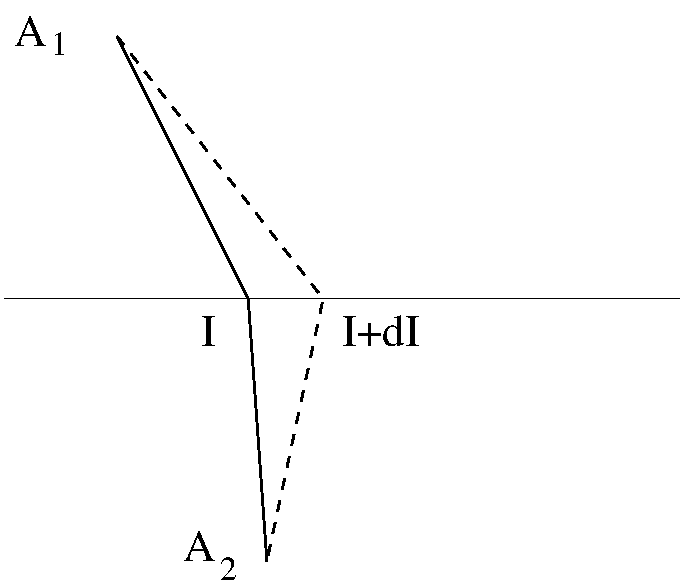
\epsfig{file={../fig/fermat},width=6 cm,angle=-90}}   
 \caption{Les lois de Descartes se d\'eduisent du principe de Fermat}
 \label{figfermat}
\end{figure}
Appliquons le principe de Fermat, c'est-\`a-dire faisons $dL=0$.
Comme $u_1$ est unitaire $\vec{u}_1.d\vec{u}_1=0$, on a :
\begin{equation}
0=(n_2u_2-n_1u_1).d\vec{I}
\end{equation}
Cette \'egalit\'e est vraie pour tout $d\vec{I}$ sur la surface :
\begin{equation}
(n_2\vec{u}_2-n_1\vec{u}_1).\vec t=0
\end{equation}
o\`u $vec t$ est un vecteur tangent \`a la surface
C'est l'\'equation de Descartes.
\end{rem}
Une autre \'equation de l'optique g\'eom\'etrique est 
l'\'equation iconale.\index{\'equation iconale}
Montrons le th\'eor\`eme suivant :
\begin{thm}
L'\'equation iconale 
\begin{equation}
n\frac{dr}{ds}=\grad\ L
\end{equation}
est \'equivalente l'\'equation du rayon lumineux :
\begin{equation}
\frac{d}{ds}(n\frac{dr}{ds})=\grad\ n
\end{equation}
\end{thm}
\begin{pf}
Diff\'erencions par rapport \`a $s$ (voir \cite{ph:optic:Born65} ) l'\'equation
iconale :
\begin{eqnarray}
\frac{d}{ds}(n\frac{dr}{ds})&=&\frac{d}{ds}\grad\ L\\
&=&\frac{dr}{ds}\grad(\grad\ L)\\
&=&\frac{1}{n}\grad\ L \grad(\grad\ L)\\
&=&\frac{1}{2n}\grad\ n^2
\end{eqnarray}
D'o\`u :
\begin{equation}
\frac{d}{ds}(n\frac{dr}{ds})=\grad\ n
\end{equation}
C'est bien l'\'equation du rayon lumineux.
\end{pf}

Le principe de Fermat est donc reli\'e aux \'equations de Maxwell {\it via}
l'\'equation iconale.

\subsection{Optique physique, Diffraction}\label{secdiffra}
%%%%%%%%%%%%%%%%%%%%%%
\subsubsection{Position du probl\`eme}
%%%%%%%%

Consid\'erons un \'ecran $S_1$ perc\'e par une
surface\index{diffraction} 
$\Sigma$. Le compl\'ementaire de $\Sigma$ dans $S_1$ est not\'e
$\Sigma^c$ (voir figure \ref{figecran}).
\begin{figure}[htb]
 \centerline{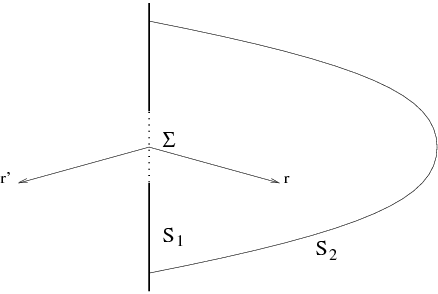
\epsfig{file={../fig/ecran},width=6 cm,angle=-90}}   
 \caption{les diff\'erentes surfaces d'int\'egration pour le probl\`eme de la diffraction.}
 \label{figecran}
\end{figure}
On suppose qu'un signal \'electromagn\'etique tombe sur l'\'ecran et
que sur $\Sigma$, le signal n'est pas p\'erturb\'e par la pr\'esence
de l'\'ecran, donc que $u$ a pour valeur la valeur $u_{libre}$
qu'aurait $u$ s'il n'y avait pas d'\'ecran. Par ailleurs, on supoose
que $u$ est nul sur le compl\'ementaire de $\Sigma$.
\'Enon\c cons le probl\`eme de la diffraction bien
formul\'e\cite{ph:optic:Goodman68} (selon Rayleigh Sommerfeld) : 
\begin{prob}
\'Etant donn\'e $u_{libre}$, trouver la fonction $u$ v\'erifiant :
\begin{equation}
 (\Delta +k^2)u=0{\rm\ dans\ }\Omega
\end{equation}
\begin{equation}
u=u_{libre} {\rm\ sur\ }\Sigma
\end{equation}
\begin{equation}
u=0{\rm\ sur\ }\Sigma^c
\end{equation}
\end{prob}
On connait la solution \'el\'ementaire de l'op\'erateur $\Delta +k^2$
dans le cas infini (sans \'ecran), pour le probl\`eme homog\`ene. C'est
:
\begin{equation}
G_M(M')=\frac{e^{jkr}}{r}
\end{equation}
o\`u $r=|MM'|$.
Mais
par la m\'ethode des images, on connait aussi la solution de Green du
probl\`eme avec \'ecran homog\`ene qui est :
\begin{prob}
Trouver la fonction $u$ v\'erifiant :
\begin{equation}
 (\Delta +k^2)u=0{\rm\ dans\ }\Omega
\end{equation}
\begin{equation}
u=0{\rm\ sur\ }S_1=\Sigma^c\cup\Sigma^c
\end{equation}
\end{prob}
Cette solution est :
\begin{equation}\label{eqgreendif}
G_M(M')=\frac{e^{jkr}}{r}+\frac{e^{jkr^s}}{r^s}
\end{equation}
avec $r_s=|M_sM'|$ o\`u $M_s$ est le sym\'etrique de $M$ par rapport
\`a l'\'ecran.
On a donc :
\begin{equation}
U(M)=\int_\Omega u(M')\delta_M(M') dM'=\int_\Omega
u(M')(\Delta+k^2)G_M(M')dM' 
\end{equation}
Or, en utilisant le fait que dans $\Omega$, $\Delta u=-k^2u$, on a :
\begin{equation}
\int_{\Omega}U(\Delta+k^2)\frac{G}{4\pi}dr=\int_{\Omega}(U\Delta
G-G\Delta U)\ dr
\end{equation}
En appliquant le th\'eor\`eme de Green, on peut
transformer l'int\'egrale de volume en int\'egrale de surface :
\begin{equation}
\int_{\Omega}(U\Delta G-G\Delta U)\ dr=\int_{\cal S}(U\frac{\partial
 G}{\partial n}-G\frac{\partial U}{\partial n}) dr
\end{equation}
L'int\'egrale sur $S=S_1+S_2$ se r\'eduit \`a une int\'egrale sur
$S_1$  si la 
condition dite {\it condition de rayonnement de
Sommerfeld}\index{Sommerfeld (condition de rayonnement de)} est
v\'erifi\'ee :
\subsubsection{Condition de rayonnement de Sommerfeld}
%%%%%%%%%%%%%%%%%%%%%%%%%%%%%%%%%%%%%%
Consid\'erons le cas particulier o\`u la surface $S_2$ est la calotte de
sph\`ere centr\'ee en P et de rayon $R$. Cherchons une condition pour que
l'int\'egrale $I$ d\'efinie par :
\begin{equation}
I=\int_{S_2}(U\frac{\partial G}{\partial n}-G\frac{\partial
U}{\partial n}) dr
\end{equation}
soit nulle lorsque $R$ tend vers l'infini.
Nous avons
\begin{equation}
\frac{\partial G}{\partial n}=(jk-\frac{1}{R})\frac{e^{jkR}}{R}\sim jkG
\end{equation}
Donc
\begin{equation}
I=\int_{\omega}\frac{e^{jkR}}{R}(\frac{\partial U}{\partial n}-jkU)R^2
d\omega
\end{equation}
o\`u $\omega$ est l'angle solide.
Si dans toutes les directions, la condition : 
\begin{equation}
\lim_{R\rightarrow\infty}R(\frac{\partial U}{\partial n}-jkU)=0
\end{equation}
est v\'erifi\'ee alors $I$ est nulle.
\begin{rem}
Si le $U$ est une superposition d'ondes sph\'eriques, cette condition est
v\'erifi\'ee\footnote{%%%%%
En effet, si $U$ s'\'ecrit :
\begin{equation}
U=\frac{e^{jkR}}{R}
\end{equation}
alors :
\begin{equation}
R(\frac{\partial U}{\partial n}-jkU)=-\frac{e^{jkR}}{R}
\end{equation}
 qui tend bien vers 0 quand $R$ tend vers l'infini.
}.
\end{rem}

\subsubsection{Principe de Huyghens}\label{secHuyghens}
%%%%%%%%%%%%%%%%%%%%%%%%
D'apr\`es l'\'equation \ref{eqgreendif}, $G$ est nulle sur $S_1$.
\index{Huyghens (principe de Huyghens)}
Nous avons donc pour $U$ :
\begin{equation}
U(M)=\frac{1}{4\pi}\int_{S_1}U(M')\frac{\partial G_M(M')}{\partial n}ds'
\end{equation}
Or :
\begin{eqnarray}
\frac{\partial G}{\partial n}&=&\cos
(n,r_{01})(jk-\frac{1}{r_{01}})\frac{e^{jkr_{01}}}{r_{01}}\\
&&-\cos(n,r'_{01})(jk-\frac{1}{r'_{01}})\frac{e^{jkr'_{01}}}{r'_{01}}
\end{eqnarray}
o\`u $r_{01}=MM'$ et $r'_{01}=M_sM'$, $M'$ appartenant \`a $\Sigma$ et
$M_s$ \'etant le sym\'etrique du point $M$ en lequel on \'evalue le
champ $u$ par rapport \`a l'\'ecran. On a donc :
\begin{equation}
r_{01}=r'_{01}
\end{equation}
et 
\begin{equation}
\cos(n,r'_{01})=-\cos(n,r_{01})
\end{equation}
D'o\`u :
\begin{equation}
\frac{\partial G}{\partial n}=
2\cos(n,r_{01})(jk-\frac{1}{r_{01}})\frac{e^{jkr_{01}}}{r_{01}}ds 
\end{equation}
D'o\`u pour $r_{01}$ grand :
\begin{equation}
U(P_0)=\int_{S_1}U(r)\frac{1}{j\lambda}\cos(n,r_{01})
\frac{e^{jkr_0}}{r_0}ds 
\end{equation}
Nous retrouvons le {\bf principe de Huyghens} :
\begin{prin}
\begin{itemize}
\item La lumi\`ere se propage de proche en proche. Chaque \'el\'ement
de surface 
atteint par elle se comporte comme une source secondaire qui \'emet des
ondelettes sph\'eriques dont l'amplitude est proportionnelle \`a cet
\'el\'ement.
\item L'amplitude complexe de la vibration lumineuse en un point est la
somme des amplitudes complexes des vibrations produites par toutes les
sources secondaires. On dit que ces vibrations interf\`erent pour former
la vibration au point consid\`ere.
\end{itemize}
\end{prin}
\begin{rem}
Nous avons montr\'e que le facteur de forme est $\frac{1}{j\lambda}$.
\end{rem}

\subsubsection{Approximations de Fresnel et de Fraunhoffer}
%%%%%%%%%%%%%%%%%%%%%%%%%%%%%%%%%%%%%
Nous supposons $\cos(n,r)\sim 1$ . Soit $O$ l'origine sur $S_1$, M un
point de $S_1$ et P le point o\`u l'on calcule le champ. On note $R=OP$,
$R_m=OM$, $r_{01}=PM$ alors faire l'approximation de
Fresnel\index{Fresnel (approximation de)} consiste a
prendre 
\begin{equation}
\frac{e^{jkr_{01}}}{r_{01}}=\frac{e^{jkR}}{R}e^{jke.R_m}e^{\frac{jke.R_m^2}{2R}}
\end{equation}
Faire l'approximation de Fraunhoffer\index{Fraunhoffer (approximation
de)}  consiste \`a prendre : 
\begin{equation}
\frac{e^{jkr_{01}}}{r_{01}}=\frac{e^{jkR}}{R}e^{jke.R_m}
\end{equation}
On observe sur l'\'ecran la transform\'ee de Fourier de l'amplitude sur
$S_1$.







\section{Interaction \'electromagn\'etique}
%%%%%%%%%%%%%%%%%%%%%%%%%%%%%%%%%%%%%%
\subsection{Forces \'electromagn\'etiques}
%%%%%%%%%%%%%%%
Dans le cas d'une particule de charge $q$ la force
\'electromagn\'etique appliqu\'ee \`a cette particule est :
\begin{equation}
f=qE+qv\wedge B
\end{equation}
o\`u $qE$ est la force \'electrique (ou de Coulomb)\index{Coulomb
(force de)} et $qv\wedge B$
est la force de Lorentz.\index{Lorentz (force de)}
Ce r\'esultat se g\'en\'eralise aux milieux continus par
l'interm\'ediaire du vecteur de Poynting.\index{Poynting (vecteur de)}
\subsection{\'Energie \'electromagn\'etique, vecteur de
Poynting}\label{secenergemag}
%%%%%%%%%%%%%%
Le postulat sur les forces peut \^etre remplac\'e par un postulat sur
les puissances en introduisant le vecteur de Poynting.
\begin{postulat}
Soit un volume $V$. Soit le vecteur $P=E\wedge H$ appel\'e vecteur de
Poynting. Nous postulons que le flux du vecteur $P$ \`a travers la
surface $S$ d\'elimitant le volume $V$, orient\'ee par une normale
rentrante est \'egal \`a la puissance \'electromagn\'etique ${\cal
P}$ apport\'ee \`a ce volume. 
\end{postulat}
\begin{equation}
{\cal P}=\intt E\wedge H n ds =-\inttt \dive (E\wedge H)d\tau
\end{equation}
\begin{equation}
{\cal P}=H\frac{\partial B}{\partial t}+E.j+E\frac{\partial
D}{\partial t}
\end{equation}
Les champs s'obtiennent \`a l'aide d'\'equations appel\'ees
\'equations de Maxwell. Montrons l'\'equivalence du point de vue des
forces et du point de vue des puissances dans le cas de la force de
Coulomb.

Consid\'erons une charge ponctuelle $q$ dans un champ $E$. D\'epla\c
cons cette charge de $dr$. Le postulat des \'equations de Maxwell nous
dit que ce d\'eplaement de charge correspons \`a une variation
d'\'energie interne 
\begin{equation}
dU=\int EdD
\end{equation}
o\`u $dD$ est la variation de $D$ induite par le d\'eplacement de la
charge.
\begin{thm}
La variation d'\'energie interne s'exprime comme :
\begin{equation}
dU=-f dr
\end{equation}
\end{thm}
\begin{pf}
\small
En \'electrostatique, le champ $E$ est \`a circulation conservative ($\rot
E=0$) donc il d\'erive d'un potentiel.
\medskip
\'Ecrivons la variation d'\'energie \'electrostatique\cite{ph:elect:Fournet}
\begin{equation}
\delta U=\int E\delta D \ d\tau
\end{equation}
\begin{equation}
\delta U=\int- \grad (V)\ \delta D \ d\tau
\end{equation}
\begin{equation}
\delta U=\int V \dive(\delta D) \ d\tau-\int \dive(V\delta D)\  d\tau
\end{equation}
Le flux relatif \`a la divergence de $V\delta D$ est nul sur tout
l'espace, en effet $D$ d\'ecro\^\i t en $1/r^2$ et $V$ en $1/r$ et la surface
croit en $r^2$. D'o\`u :
\begin{equation}
\delta U=\int V \delta \rho \ d\tau
\end{equation}
D\'epla\c cons une charge de la quantit\'e $\delta r$. La distribution de
charge passe donc de $q\delta(r)$ \`a $q\delta(r+dr)$ o\`u
$\delta(r)$ est la distribution de Dirac. Nous avons donc $d
\rho(r)=q(\delta(r+\delta r)-\delta(r))$. D'o\`u :
,\begin{equation}
dU=\inttt qV(r)(\delta(r+\delta r)-\delta(r)) \ d\tau
\end{equation}
donc
\begin{equation}
\delta U=qV(r+\delta r)-qV(r))
\end{equation}
\begin{equation}
\delta U=\grad(qV)\delta r
\end{equation}
La variation est bien de la forme voulue $\delta U=-fdr$. De plus on a
montr\'e que :
\begin{equation}
f=-\grad(qV)=qE
\end{equation}    
\end{pf}


\section{Exercices}
%%%%%%%%%%%%%%%%%%%%%

\begin{exo}
D\'emontrer l'\'equation \ref{eqconsdelacharge} de la conservation de la
charge \`a partir des \'equations de Maxwell.
\end{exo}

\begin{exo}
Donner l'expression du potentiel cr\'ee par un quadrip\^ole $Q_{ij}$.
\end{exo}

\begin{exo}
Montrer \`a partir de l'expression de l'\'energie magn\'etique que la force
magn\'etique agissant sur une charge ponctuelle $q$ de vitesse $v$ a pour
expression : 
\begin{equation}
f=qv\wedge B
\end{equation}

\end{exo}

\chapter{M\'ecanique Quantique}\label{chapmq}
%%%%%%%%%%%%%%%%%

\section{Introduction}
%%%%%%%%%%%%%%%%%%%
Dans l'\'etat actuel des connaissances scientifiques, la physique
quantique est la th\'eorie utilis\'ee pour la description et la
compr\'ehension des ph\'enom\`enes qui se produisent \`a tr\`es petite
\'echelle (atomique ou subatomique).
Le but de ce chapitre est de pr\'esenter le formalisme math\'ematique
de la m\'ecanique quantique.
Des applications de la m\'ecanique quantique seront vues au chapitre
\ref{chapproncorps}.
La physique quantique repose sur une s\'erie de postulats que nous
pr\'esentons maintenant.
 Nous renvoyons \`a
\cite{ph:mecaq:Cohen73,ph:mecaq:Bohm93} pour 
toutes les justifications physiques.
\section{Postulats}
%%%%%%%%%%%%%%%%%%%%%%%%%%%%%%

\subsection{Espace des \'etats}
%%%%%%%%%
Le premier postulat concerne la description de l'\'etat d'un
syst\`eme. 
\begin{postulat}
(Description de l'\'etat d'un syst\`eme) \`A tout syst\`eme physique
quantique correspond un espace de Hilbert 
${\cal H}$ complexe \`a base d\'enombrable.
\end{postulat}
L'espace ${\cal H}$ doit \^etre pr\'ecis\'e pour chaque syst\`eme
physique \'etudi\'e.
\begin{exmp}
Pour un syst\`eme constitu\'e par une particule \`a spin nul dans une
th\'eorie non relativiste, on adopte pour espace de Hilbert ${\cal H}$ l'espace $L^2(R^3)$. C'est l'espace des fonctions complexes sur
$R^3$ de carr\'e int\'egrable (relativement \`a la mesure de Lebesgue)
muni du produit scalaire :
\begin{equation}
<\phi|\psi>=\int \phi(x)\bar\psi(x) dx
\end{equation}
Cet espace est appel\'e espace des \'etats orbitaux.\index{espace des
\'etats} 
\end{exmp}
La m\'ecanique quantique substitue donc \`a la notion classique de
position et vitesse de particule une fonction $\psi(x)$ de carr\'e
sommable. Un \'el\'ement $\psi(x)$ de $\cal H$ est not\'e $|\psi>$ en
notations de Dirac.
\begin{exmp}
Pour un syst\`eme constitu\'e par une particule de spin
\index{spin}$s$ non--nul dans un th\'eorie non relativiste, l'espace
des \'etats est le produit 
tensoriel $L^2(R^3)\otimes C^n$ o\`u $n=2s+1$.
Les particules de spin entier sont appel\'ees bosons;\index{bosons}
les particules 
de spin demi-entier sont appel\'ees fermions.\index{fermions} 
\end{exmp}
\begin{exmp}
Pour un syst\`eme constitu\'e de $N$ particules distinctes, l'espace
des \'etats est le produit tensoriel des espaces de Hilbert $h_i$ ($i
\in (1,\dots,N)$)
o\`u $h_i$ est l'espace de Hilbert associ\'e \`a la particule $i$.
\end{exmp}
\begin{exmp}\label{exmppauli}
Pour un syst\`eme constitu\'e de $N$ particules identiques 
l'espace des \'etats est un sous--espace de
$\otimes_{i=1}^N h_i$ o\`u $h_i$ est l'espace de Hilbert associ\'e \`a
la particule $i$.
Soit $\psi_{\alpha_1,\dots,\alpha_N}$ une fonction de ce sous--espace. On peut
\'ecrire :
\begin{equation}
\psi_{\alpha_1,\dots,\alpha_N} = \phi_{\alpha_1}(1)\otimes \dots
\otimes\phi_{\alpha_2}(N) 
\end{equation}
o\`u $\phi_{\alpha_i}\in h_i$.
Soit $P^{\pi}$ l'op\'erateur permutation\index{permutation} de
$\otimes_{i=1}^N h_i$ dans 
$\otimes_{i=1}^N h_i$ d\'efini par :
\begin{equation}
P^{\pi}(\psi_{\alpha_1,\dots,\alpha_N})=
\phi_{\alpha_1}(\pi(1))\otimes \dots 
\otimes\phi_{\alpha_2}(\pi(N)) 
\end{equation}
o\`u $\pi$ est une permutation de $(1,\dots,N)$.
On appelle un vecteur sym\'etrique un vecteur de la forme :
\begin{equation}
\phi^s=\frac{1}{k^s}\sum_\pi P^\pi(\psi_{\alpha_1,\dots,\alpha_N})
\end{equation}
On appelle un vecteur antisym\'etrique un vecteur de la forme :
\begin{equation}
\phi^a=\frac{1}{k^a}\sum_\pi (-1)^{p_\pi}
P^\pi(\psi_{\alpha_1,\dots,\alpha_N}) 
\end{equation}
o\`u $(-1)p_\pi$ est la signature \index{signature} (ou parit\'e) de la
permutation $\pi$, $p_\pi$ \'etant le nombre 
de transpositions dont la permutation $\pi$ est le produit.
Les coefficients $k^s$ et $k^a$ permettent de normaliser les fonctions
d'ondes; la somme
s\'etend \`a toute les permutations  $\pi$ de $(1,\dots,N)$.
Suivant la nature des particules, c'est soit les vecteurs sym\'etriques, soit
les vecteurs antisym\'etriques qui sont des vecteur d'\'etat. Plus
pr\'ecisemment :
\begin{itemize}
\item Pour les bosons, l'espace des \'etats est le sous--espace de
$\otimes_{i=1}^N h_i$ constitu\'e par les vecteurs sym\'etriques.
\item Pour les fermions, l'espace des \'etats est le sous--espace de
$\otimes_{i=1}^N h_i$ constitu\'e par les vecteurs anti--sym\'etriques.
\end{itemize}
\end{exmp}
Pour \'enoncer les postulats suivants, il nous faut d\'efinir une
``repr\'esentation'' \cite{ma:equad:Dautray5,ph:mecaq:Cohen73}.
\subsection{Repr\'esentation Schr\"odinger}
%%%%%%
Voici l'\'enonc\'e des quatre postulats suivants dans la
repr\'esentation de Schr\"odinger.\index{Schr\"odinger
(repr\'esentation de)}
\begin{postulat}
(Description des grandeurs physiques) Toute grandeur physique
mesurable $\cal A$ est d\'ecrite par un 
op\'erateur $A$ agissant dans $\cal H$. Cet op\'erateur est une
observable.
\end{postulat}
\begin{postulat}
(R\'esultat possible)
La mesure d'une grandeur physique $\cal A$ ne peut donner comme
r\'esultat qu'une des valeurs propres de l'observable $A$
correspondante.
\end{postulat}
\begin{postulat}(Principe de d\'ecomposition spectrale)
Lorsqu'on mesure la grandeur physique $\cal A$ sur un syst\`eme dans
l'\'etat $|\psi \rangle $ norm\'e, la valeur moyenne des mesures est
$<A>$ :
\begin{equation}
<A>=<\psi|A\psi>
\end{equation}
o\`u $<\ .\ |\ .\ >$ repr\'esente le produit scalaire dans $\cal H$. 
En particulier, si $A=\sum |v_i>a_i<v_i|$, la probabilit\'e d'obtenir
la valeur $a_i$ lors d'une mesure est :
\begin{equation}
P(a_i)=<\psi|v_i><v_i|\psi>
\end{equation}
\end{postulat}
\begin{postulat}
(\'Evolution)
L'\'evolution du vecteur d'\'etat $\psi(t)$ est r\'egie par
l'\'equation de 
Schr\"odinger :
\begin{equation}
i\hbar \frac{d}{dt} \psi(t)\rangle =H(t)|\psi(t)\rangle 
\end{equation}
o\`u $H(t)$ est l'observable associ\'ee \`a l'\'energie du syst\`eme.
\end{postulat}
\begin{rem}
On peut exprimer l'\'etat \`a l'instant $t$ en fonction de l'\'etat
\`a l'instant $0$:
\begin{equation}
|\psi(t)\rangle=U|\psi(0)\rangle
\end{equation}
L'op\'erateur $U$ est appel\'e op\'erateur
d'\'evolution.\index{op\'erateur d'\'evolution} On peut
montrer que $U$ est unitaire.\index{op\'erateur unitaire}
\end{rem}
\begin{rem}
Lorsque l'op\'erateur $H$ ne d\'epend pas du temps, l'\'equation
d'\'evolution s'int\`egre facilement et on obtient :
\begin{equation}
|\psi(t)\rangle=U|\psi(0)\rangle
\end{equation}
avec 
\begin{equation}
U=e^{-iHt/\hbar}
\end{equation}
Lorsque $H$ d\'epend du temps la solution de l'\'equation:
\begin{equation}
i\hbar \frac{\partial U(t)}{\partial t}=H(t)U(t)
\end{equation}
n'est pas :
\begin{equation}
U(t)=e^{\frac{i}{\hbar}\int_0^t H(t')dt'}
\end{equation}
\end{rem}
Les r\`egles de quantification nous donnerons un moyen d'exprimer
l'\'energie.
\subsection{Autres repr\'esentations}\label{secautresrep}
%%%%%%%%%%%%%%%%%%%%%%%
On obtient d'autres repr\'esentations par transformation unitaire.
\begin{defn}
 Par d\'efinition\cite{ph:mecaq:Cohen73}, un op\'erateur $U$ est unitaire si son inverse
$U^{-1}$ est \'egal a son adjoint $U^+$
\begin{equation}
U^+U=UU^+=1
\end{equation}
\end{defn}
\begin{prop}
 Si $A$ est hermitique,  alors l'op\'erateur $T=e^{iA}$ est
unitaire
\end{prop}
En effet :
\begin{equation}
T^+=e^{-iA^+}=e^{-iA}
\end{equation}
\begin{equation}
T^+T=e^{-iA}e^{+iA}=1
\end{equation}
\begin{equation}
TT^+=e^{iA}e^{-iA}=1
\end{equation}
\begin{prop}
La transformation unitaire conserve le produit
scalaire
\end{prop}
\begin{pf} En effet, si 
\begin{equation}
\tilde{\psi_1}=U\psi_1 {\rm\ et\ } \tilde{\psi_2}=U\psi_2
\end{equation}
alors
\begin{equation}
 \langle \psi_1|\psi_2\rangle = \langle \tilde{\psi_1}|\tilde{\psi_2}\rangle 
\end{equation} 
\end{pf}
\subsection{Repr\'esentation d'Heisenberg}
%%%%%%%%%%%%%%%%%%%%%%%%%%%%%%
On a vu que l'op\'erateur d'\'evolution donne l'\'etat \`a l'instant
$t$ en fonction de l'\'etat \`a l'instant $0$ :
\begin{equation}
\phi(t)=U\phi(0)
\end{equation}
Notons $\phi_S$ l'\'etat en repr\'esentation de Schr\"odinger et
$\phi_H$ l'\'etat en repr\'esentation de Heisenberg.\index{Heisenberg
(repr\'esentation d')}
La repr\'esentation de Heisenberg est d\'efini \`a partir de la
repr\'esention de Schr\"odinger par la transformation unitaire
suivante :
\begin{equation}
\phi_H=V\phi_S
\end{equation}
avec 
\begin{equation}
V=U^{-1}
\end{equation}
Autrement dit, l'\'etat en repr\'esentation de Heisenberg est
caracteris\'e par une fonction d'onde ind\'ependante de $t$ et \'egale
\`a l'\'etat correspondant en repr\'esentation de Schr\"odinger pour
$t=0$ : $\phi_H=\phi_S(0)$.
Ceci nous am\`ene donc \`a changer le postulat sur les observables:
\begin{postulat}(Description des grandeurs physiques)
\`A toute grandeur physique auquel correspond un espace de Hilbert
${\cal H}$ est associ\'ee une fonction $t\in R\rightarrow A_H(t)$ \`a
valeurs d'op\'erateurs autoadjoints $A_H(t)$ dans ${\cal H}$.
\end{postulat}
Si on note $A_S$ l'op\'erateur associ\'e \`a une grandeur physique
$\cal A$ en repr\'esentation de Schr\"odinger alors le lien entre $A_S$
et $A_H$ est :
\begin{equation}
A_H(t)=U^+A_SU
\end{equation}
On constate que $A_H$ d\'epend du temps m\^eme si $A_S$ est
ind\'ependant du temps.
\begin{postulat}(R\'esultat possible)
La valeur d'une grandeur physique \`a l'instant $t$ ne peut \^etre que
l'un des points du spectre de l'op\'erateur autoadjoint $A(t)$ qui lui
est associ\'e.
\end{postulat}
Le principe de d\'ecomposition spectrale reste inchang\'e :
\begin{postulat}(Principe de d\'ecomposition spectrale)
Lorsqu'on mesure la grandeur physique $\cal A$ sur un syst\`eme dans
l'\'etat $|\psi_H \rangle $ norm\'e, la valeur moyenne des mesures est
$<A_H>$ :
\begin{equation}
<A>=<\psi_H|A_H\psi_H>
\end{equation}
\end{postulat}
Le lien avec la repr\'esentation de Schr\"odinger est d\'ecrit par la
relation suivante :
\begin{equation}
<\psi_H|A_H\psi_H>=<\psi_SU|U^+A_SU|U^+\psi_H>
\end{equation}
Comme $U$ est unitaire :
\begin{equation}
<\psi_H|A_H\psi_H>=<\psi_S|A_S\psi_S>
\end{equation}
Le postulat sur la probabilit\'e d'obtenir une valeur pour une
mesure est le m\^eme, sauf que c'est l'op\'erateur qui d\'epend du
temps et pas le vecteur.
\begin{postulat}(\'Evolution)
L'\'equation d'\'evolution est (dans le cas d'un syst\`eme isol\'e) :
\begin{equation}
i\hbar \frac{dA}{dt}(t)=-(HA(t)-A(t)H)=-[H,A(t)]
\end{equation}
\end{postulat}
Cette \'equation est appel\'ee \'equation de Heisenberg pour les
observables. 
\begin{rem}
Si le syst\`eme est conservatif ($H$ ne d\'epend pas du temps), alors
on a vu que 
\begin{equation}
U=e^{-iHt/\hbar}
\end{equation}
Si nous associons \`a une grandeur physique au temps $t=0$
l'op\'erateur $A(0)=A$ identique \`a l'op\'erateur associ\'e \`a cette
grandeur dans la repr\'esentation de Schr\"odinger, l'op\'erateur
$A(t)$ s'\'ecrit:
\begin{equation}
A(t)=e^{+i\frac{Ht}{\hbar}}A e^{-i\frac{Ht}{\hbar}}
\end{equation}
\end{rem}
\subsection{Repr\'esentation d'interaction}
%%%%%%%%%%%%%%%%%%%%%%%
Supposons que l'hamiltonien $H$ se d\'ecompose en deux termes $H_0$ et
$H_i$. En pratique $H_i$ est souvent consid\'er\'e comme une perturbation
de $H_0$ et repr\'esente un terme d'interaction.
Notons $|\psi_S\rangle $ un \'etat dans la repr\'esentation de
Schr\"odinger et 
$|{\psi}_I\rangle $ un \'etat dans la repr\'esentation
d'interaction.\index{interaction (repr\'esentation d')}
\begin{equation}
|{\psi}_I\rangle =U_0|\psi_S\rangle
\end{equation}
avec 
\begin{equation}
U_0=e^{iH_0t/\hbar}
\end{equation}
\begin{postulat}(Description des grandeurs physiques)
\`A toute grandeur physique auquel correspond un espace de Hilbert
${\cal H}$ est associ\'ee une fonction $t\in R\rightarrow A_I(t)$ \`a
valeurs d'op\'erateurs autoadjoints $A_I(t)$ dans ${\cal H}$.
\end{postulat}
Si on note $A_S$ l'op\'erateur associ\'e \`a une grandeur physique
$\cal A$ en repr\'esentation de Schr\"odinger alors le lien entre $A_S$
et $A_I$ est :
\begin{equation}
A_I(t)=U_0A_SU_0^+=e^{iH_0t/\hbar}A_S e^{-iH_0t/\hbar}
\end{equation}
On constate que $A_I$ d\'epend du temps m\^eme si $A_S$ est
ind\'ependant du temps.
Le postulat sur les r\'esultats possibles reste inchang\'e.
\begin{postulat}
Lorsque l'on mesure la grandeur physique $\cal A$ dans l'\'etat $\psi_I$,
la valeur moyenne de $A_I$ est:
\begin{equation}
<\psi_I|A_I\psi_I>
\end{equation}
\end{postulat}
Comme on l'a fait pour la repr\'esentation de Heisenberg, on peut
montrer que c'est le m\^eme r\'esultat que dans la repr\'esentation de
Schr\"odinger.
De l'\'equation de Schr\"odinger, on d\'eduit imm\'ediatement l'\'equation
d'\'evolution dans la repr\'esentation d'interaction.
\begin{postulat}(\'Evolution)
L'\'evolution d'un vecteur $\psi_I$ est donn\'ee par :
\begin{equation}
i\hbar \frac{d}{dt} |\psi_I(t)\rangle
= V_I|\psi_I(t)\rangle  
\end{equation}
avec
\begin{equation}
V_I=e^{iH_0t/\hbar}H_ie^{-iH_0t/\hbar}
\end{equation}
\end{postulat}
La repr\'esentation d'interaction facilite les calculs perturbatifs.
Elle est utilis\'ee par exemple en \'electrodynamique
quantique\cite{ph:mecaq:Cohen88}.
Dans la suite nous utiliserons uniquement la repr\'esentation de
Schr\"odinger.
\section{Principales  observables}
%%%%%%%%%%%%%%%%
\subsection{Op\'erateurs hamiltoniens}
%%%%%%%%%%%%%%%%%%%%%%%%%%%%%%%%
L'op\'erateur hamiltonien \index{hamiltonien (op\'erateur)} a \'et\'e
d\'efini comme le g\'en\'erateur 
infinit\'esimal multipli\'e par $i\hbar$ du groupe d'\'evolution.
L'exp\'erience, les m\'ethodes de passage de la m\'ecanique classique
\`a la m\'ecanique quantique permettent de donner son expression pour
chaque syst\`eme physique \'etudi\'e.
L'invariance de l'\'equation de Schr\"odinger par rotation implique que
l'hamiltonien est un op\'erateur scalaire (invariant par rotation)
(voir annexe \ref{chapgroupes}).
\begin{exmp}
Ainsi si l'\'energie classique d'une particule est :
\begin{equation}
E_c=\frac{p^2}{2m}
\end{equation}
son \'equivalent quantique l'hamiltonien $H$ s'\'ecrira :
\begin{equation}
H=\frac{P^2}{2m}
\end{equation}
\end{exmp}
\begin{rem}{\bf R\`egles de quantification}
Les r\`egles de quantification \cite{ph:mecaq:Cohen73} indiquent, comment pour
une grandeur physique ${\cal A}$ d\'ej\`a d\'efinie en m\'ecanique
classique, on construit un op\'erateur $A$ qui la d\'ecrit en
m\'ecanique quantique. 
\end{rem}
\subsection{Op\'erateur position}
%%%%%%%%%%%%%%%%%%%%%%%%%%

La notion classique de position $r$ d'une particule am\`ene \`a
associer \`a une particule un ensemble de trois op\'erateurs (observables)
$R_x,R_y,R_z$ appel\'es op\'erateurs position\index{position (op\'erateur)} et d\'efinis par :

\begin{equation}
R_x\phi(x,y,z)=x\phi(x,y,z)
\end{equation}

\begin{equation}
R_y\phi(x,y,z)=y\phi(x,y,z)
\end{equation}

\begin{equation}
R_z\phi(x,y,z)=z\phi(x,y,z)
\end{equation}

\subsection{Op\'erateur impulsion}
%%%%%%%%%%%%%%%%%%%%%%%%%%%%%%%
De m\^eme, \`a la l'impulsion $p$ ``classique'' de la particule on
associe l'observable $P=(P_x,P_y,P_z)$. L'action de l'op\'erateur
$P_x$ est d\'efinie par \index{impulsion (op\'erateur)}:
\begin{equation}
P_x\phi=\frac{\hbar}{i}\frac{\partial}{\partial x} \phi
\end{equation}
Les op\'erateurs 
$R$ et $P$ v\'erifient les relations de commutation suivantes dites
{\bf relations de commutation canoniques}\index{relations
de commutation} :
\begin{equation}
[R_i,R_j]=0
\end{equation}
\begin{equation}
[P_i,P_j]=0
\end{equation}
\begin{equation}
[R_i,P_j]=i\hbar \delta_{ij}
\end{equation}
o\`u $\delta_{ij}$ est le symbole de Kronecker (voir l'annexe
\ref{secformultens}).
De mani\`ere g\'en\'erale, l'observable $A$ associ\'ee \`a une
grandeur physique $\cal A$ d\'efinie classiquement s'obtient en
rempla\c cant, dans l'expression convenablement sym\'etris\'ee de
$\cal A$, r et p par les observables $R$ et $P$.
\subsection{Op\'erateurs moment cin\'etique}
%%%%%%%%%%%%%%%%%%%%%%%%%%%%%
\begin{defn}
On appel\'e moment cin\'etique\index{moment cin\'etique (op\'erateur)}
$J$, un ensemble de trois observables 
$J_x,J_y,J_z$ v\'erifiant les relations de commutation\index{relations
de commutation} suivantes :
\begin{equation}
[J_i,J_l]=i\hbar\epsilon_{kil}J_k
\end{equation}
c'est-\`a-dire :
\begin{equation}
[J_x,J_y]=i\hbar J_z
\end{equation}
\begin{equation}
[J_y,J_z]=i\hbar J_x
\end{equation}
\begin{equation}
[J_z,J_x]=i\hbar J_y
\end{equation}
o\`u $\epsilon_{ijk}$ est le tenseur signature des permutations (voir l'annexe
\ref{secformultens}).
\end{defn}
\begin{exmp}
{\bf Moment cin\'etique orbital}
\begin{thm}
L'op\'erateur d\'efini par $L_i=\epsilon_{ijk}R_jP_k$ est un moment
cin\'etique; il est appel\'e moment cin\'etique orbital.
\end{thm}
\begin{pf}
\'Evaluons\cite{ph:mecaq:Bohm93} le commutateur :
\begin{eqnarray}
[L_i,L_l]&=&\epsilon_{ijk}\epsilon_{lmn}(x_jp_kx_mp_n-x_mp_nx_jp_k)\\
&=&i\hbar
\epsilon_{ijk}\epsilon_{lmn}(\delta_{km}x_jp_n-\delta_{nj}x_mp_k)\\ 
&=&i\hbar \epsilon_{ijk}\epsilon_{lkn}x_jp_n -
\epsilon_{ijk}\epsilon_{lmj}x_mp_k 
\end{eqnarray}
o\`u on a utilis\'e les relations de commutation canoniques.
Soit en changeant de notation ;
\begin{eqnarray}
[L_i,L_l]&=&i\hbar \epsilon_{imk}\epsilon_{lkn}x_mp_n -
\epsilon_{ijn}\epsilon_{lmj}x_mp_n\\
&=&i\hbar x_mp_n(\delta_{in}\delta_{ml}-\delta_{nl}\delta_{im})\\
&=&i\hbar x_mp_n\epsilon_{ikl}\epsilon_{knm}
\end{eqnarray}
\end{pf}
\begin{postulat}
Au moment cin\'etique orbital est associ\'e un moment magn\'etique $M$:
\begin{equation}
M=\frac{\mu_B}{\hbar}L
\end{equation}
\end{postulat}
\end{exmp}
\begin{exmp}
{\bf Postulats pour l'\'electron.}
On a vu que la description de l'\'electron doit \^etre faite dans un
espace des \'etats qui est le produit tensoriel de l'espace des
\'etats orbitaux et de l'espace des \'etats de spin.
On d\'efinit un op\'erateur $S$ appel\'e op\'erateur spin qui agit
dans l'espace des \'etats de spin.
On postule que cet op\'erateur est un moment cin\'etique et qu'il
intervient dans un hamiltonien sous la forme d'un moment magn\'etique.
\begin{postulat}
L'op\'erateur $S$ est moment cin\'etique.
\end{postulat}
\begin{postulat}
L'\'electron est une particule de spin $s=1/2$ et il poss\`ede un moment
magn\'etique \index{moment magn\'etique}intrins\`eque :
\begin{equation}
M_S=2\frac{\mu_b}{\hbar}S
\end{equation}
\end{postulat}
\end{exmp}


\subsection{R\'eponse lin\'eaire en m\'ecanique quantique}\label{secreplinmq}
%%%%%%%%%%%%%%%%%%%%%%%%%%%%%%%%%%
Soit $ \langle A\rangle (t)$ la moyenne d'un l'op\'erateur $A$
(observable). Cette 
moyenne est la quantit\'e accessible par l'exp\'erimentateur (voir
\cite{ph:mecaq:Cohen73}).
Le cas o\`u $H(t)$ est proportionnel \`a $sin(\omega t)$ est \'etudi\'e dans \cite{ph:mecaq:Cohen73}
Le cas o\`u $H(t)$ est proportionnel \`a $\delta(t)$ est celui que
nous pr\'esentons ici (voir aussi \cite{ph:physt:Noziere}). 
On \'etudie le probl\`eme :
\begin{prob}
Trouver $\psi$ tel que :
\begin{equation}
i\hbar \frac{d\psi}{dt}=(H_0+W_i(t))\psi
\end{equation}
avec
\begin{equation}
W_i(t)=W_i^c.\delta(t)
\end{equation}
et \'evaluer 
\begin{equation}
 \langle qZ\rangle = \langle \psi|qZ|\psi\rangle 
\end{equation}
\end{prob}
\begin{rem}
On peut mod\'eliser la  r\'eponse lin\'eaire dans le cadre classique
(susceptibilit\'e \'electrique, magn\'etique).
\end{rem}
Dans la repr\'esentation d'interaction\footnote{%%%%%%
Ce changement de repr\'esentation est l'\'equivalent d'une m\'ethode
WKB. En 
effet $\tilde{\psi(t)}$ devient une fonction lentement variable de $t$
puisque toute la d\'ependance temporelle est absorb\'ee par
l'op\'erateur $e^{\frac{iH_0t}{\hbar}}$}%%%%%%%%%%% 
\begin{equation}
\tilde{\psi(t)}=e^{\frac{iH_0t}{\hbar}}\psi(t)
\end{equation}
et
\begin{equation}
\tilde{W}_i(t)=e^{\frac{iH_0t}{\hbar}}W_ie^{\frac{-iH_0t}{\hbar}}
\end{equation}
La quantit\'e $ \langle qZ\rangle $ que l'on cherche \`a \'evaluer est
\'egale a : 
\begin{equation}
 \langle qZ\rangle = \langle \tilde{\psi}|q\tilde{Z}|\tilde{\psi}\rangle 
\end{equation}
\begin{equation}
i\hbar \frac{d\tilde{\psi}}{dt}=\tilde{W}_i(t)\tilde{\psi}
\end{equation}
\`A l'ordre 0 :
\begin{equation}
 \frac{d\tilde{\psi}}{dt}=0
\end{equation}
D'o\`u 
\begin{equation}
\tilde{\psi}^0(t)=\tilde{\psi}^0(0)
\end{equation}
Or $\tilde{\psi}$ a \'et\'e pr\'epar\'e dans $\psi_0$ donc :
\begin{equation}
\tilde{\psi}^0(t)=\psi_0(t)
\label{pert1}
\end{equation}
\`A l'ordre 1 on a :
\begin{equation}
\tilde{\psi}^1(t)=\tilde{\psi}^1(0)+\frac{1}{i\hbar}\int_0^t\tilde{W}_i(t\prime)\tilde{\psi}^0(t\prime)dt\prime
\end{equation}
donc d'apr\`es les propri\'et\'es de $\delta$ :
\begin{equation}
\tilde{\psi}^1(t)=\frac{1}{i\hbar}W^i_c\psi_0
\label{pert2}
\end{equation}
Calculons maintenant la valeur moyenne :
En se limitant \`a l'ordre 1, (on \'etudie la r\'eponse lin\'eaire en
E), on \'evalue :
\begin{eqnarray}
 \langle qZ\rangle &=& \langle
\tilde{\psi}^0+\tilde{\psi^1}|e^{\frac{iH_0t}{\hbar}}
qZe^{\frac{iH_0t}{\hbar}}|\tilde{\psi}^0+\tilde{\psi^1}\rangle 
\\ 
&=& \langle \tilde{\psi}^0|
e^{\frac{iH_0t}{\hbar}}qZe^{\frac{iH_0t}{\hbar}}|\tilde{\psi}^1\rangle
+ \langle
\tilde{\psi}^1|e^{\frac{iH_0t}{\hbar}}
qZe^{\frac{iH_0t}{\hbar}}|\tilde{\psi}^0\rangle 
\end{eqnarray}
En effet $ \langle \tilde{\psi}^0|qZ|\tilde{\psi}^0\rangle $ est nul
car Z est impair. 
\begin{eqnarray}
\lefteqn{ \langle
\tilde{\psi}^0|e^{\frac{iH_0t}{\hbar}}qZ
e^{\frac{iH_0t}{\hbar}}|\tilde{\psi}^1\rangle 
=}\\ 
&=& \langle {\tilde{\psi}}^0|
e^{\frac{iH_0t}{\hbar}}qZe^{\frac{-iH_0t}{\hbar}}|{\psi}_k\rangle
\langle {\psi}_k|{\tilde{\psi}}^1\rangle  
\end{eqnarray}
O\`u on a introduit une relation de fermeture. Donc en utilisant les
r\'esultats du calcul perturbatif \ref{pert1} et \ref{pert2} :
\begin{equation}
 \langle \tilde{\psi}^0|qZ|\tilde{\psi}^1\rangle =e^{i\omega_{0k}t} \langle {\psi}^0|qZ|{\psi}^k\rangle \frac{1}{i\hbar} \langle {\psi}^k|W^c_i|{\psi}^0\rangle 
\end{equation}
Nous avons donc :
\begin{eqnarray}
 \langle qZ\rangle (t)&=& 0 {\rm\ pour\ t \langle 0}\\
 \langle qZ\rangle (t)&=&
e^{i\omega_{0k}t} \langle {\psi}^0|qZ|{\psi}^k\rangle \frac{1}{i\hbar} \langle {\psi}^k|W^c_i|{\psi}^0\rangle +CC
{\rm\ sinon}
\end{eqnarray}
D'o\`u par transform\'ee de Fourier\footnote{La transform\'ee de
Fourier de :
\begin{equation}
f(t)=e^{-i\omega_0t}
\end{equation}
et celle de 
\begin{equation}
g(t)=H(t)e^{-i\omega_0t}
\end{equation}
sont diff\'erentes (celle de f(t) n'existe pas !\cite{ma:distr:Petit91})
}%%%%%%%%%%%%%%%%%%
 :
\begin{equation}
\langle qZ\rangle (\omega)=2q^2E\sum_{k\neq 0}\omega_{0k}\frac{| \langle \psi_0|Z|\psi_k\rangle |^2}{\omega_{k0}^2-\omega^2}
\end{equation}


\section{Exercices}
%%%%%%%%%%%%%%%%%%%
\begin{exo}
\'Etudier le lien des op\'erateurs position $R_x$ et impulsion $P_x$ avec le
g\'en\'erateur infinit\'esimal du groupe des translations (voir
\cite{ma:equad:Dautray5}. 
\end{exo}

\begin{exo}
\'Etudier le lien entre l'op\'erateurs moment cin\'etique $L$ et le
g\'en\'erateur infinit\'esimal du groupe des rotations (voir
\cite{ma:equad:Dautray5}.
\end{exo}

\begin{exo}
\'Etudier la r\'eponse lin\'eaire d'un oscillateur classique dont l'\'equation
est :
\begin{equation}
\frac{d^{2}x}{dt^{2}}+\gamma \frac{dx}{dt}+\omega_{0}^{2}x=f(t)
\end{equation}
o\`u $f(t)$ est l'excitation.
Comparer avec les r\'esultats obtenu \`a la section \ref{secreplinmq}.
\end{exo}

\chapter{Probl\`emes \`a N corps en m\'ecanique
quantique}\label{chapproncorps} 
%%%%%%%%%%%%%%%%%%%%%%%%%%%%%%%%%%%%%%%
\section{Introduction}
%%%%%%%%%%%%%%%%%%%%%%%
Nous traitons dans ce chapitre des probl\`emes \`a $N$ corps que la
m\'ecanique quantique permet d'aborder. Dans les atomes, les
\'el\'ements en interaction sont le noyau de l'atome et les \'electrons.
Dans une mol\'ecule, il s'agit de plusieurs noyaux et ainsi que des
\'electrons. Enfin le solide est un arrangement p\'eriodique d'atomes.
Nous ne d\'ecrivons ici que les propri\'et\'es des modes spectraux de
ces syst\`emes. Les propi\'etes thermodynamique des ensembles d'atomes
et de mol\'ecules seront \'etudi\'ees au chapitre suivant.
Sur le plan math\'ematique, ce chapitre est une illustration de la m\'ethode
spectrale pour les probl\`emes d'\'evolution lin\'eaires, pr\'esent\'ee \`a la
section \ref{chapmethspec}.
\section{Les atomes}\label{secatomemq}
%%%%%%%%%%%%%%%%%%
\subsection{Un noyau, un \'electron}\label{sechydrog}
%%%%%%%%%%%%%%%%
Ce cas correspond \`a l'\'etude de l'atome d'hydrog\`ene.\index{atome} Il s'agit du
probl\`eme d'une particule dans un potentiel central et on applique la
th\'eorie expos\'ee en \ref{secpotcent}. Le potentiel prend ici la
valeur :
\begin{equation}
V(r)=-\frac{e}{r^2}
\end{equation}
On peut montrer que les valeurs propres qui d\'ependent en g\'en\'eral
des deux nombres quantiques $k$ et $l$ ne d\'ependent pour
l'hydrog\`ene que du nombre $n=k+l$.





\subsection{Invariance par rotation}\label{secpotcent}
%%%%%%%%%%%%%%%%%%%%%%%%%%%%%%%%%%%%%%%%%%%%%
Traitons le probl\`eme de la particule dans un potentiel central
\cite{ph:mecaq:Cohen73,ma:equad:Dautray5,ph:elect:Jackson75}
Nous cherchons \`a r\'esoudre le probl\`eme spectral :
\begin{equation}
-[\frac{\hbar^2}{2\mu}\Delta+V(r)]\phi(r)=E\phi(r)
\end{equation}
Nous allons exprimer l'op\'erateur laplacien en fonction de $L^2$.
\begin{thm}
L'op\'erateur laplacien $\Delta$ s'exprime en fonction de
l'op\'erateur  $L^2$ :
\begin{equation}
\Delta=-\frac{1}{r^2}L^2+\frac{\partial^2}{\partial r^2}+\frac{2}{r}
\end{equation}
\end{thm}
\begin{pf}
Nous allons utiliser les notations tensorielles (convention d'Einstein)
Par d\'efinition :
\begin{equation}
L_i=\epsilon_{ijk}x_jp_k
\end{equation}
Puis :
\begin{eqnarray}
L_iL_i&=&\epsilon_{ijk}\epsilon_{ilm}x_{j}p_k x_l p_m\\
&=&(\delta_{jl}\delta_{km}-\delta_{jm}\delta{kl})x_{j}p_kx_l p_m\\
&=&x_jx_jp_kp_k-x_jp_kx_kp_j
\end{eqnarray}
Nous faisons attention \`a l'ordre dans lequel sont ecrits les
op\'erateurs car nous avons les relations de commutation canoniques :
\begin{equation}
[x_i,p_j]=i \hbar \delta_{ij}
\end{equation}
\begin{equation}
[x_j,x_k]=0
\end{equation}
\begin{equation}
[p_j,p_k]=0
\end{equation}
Nous avons 
\begin{equation}
p_k=-i\frac{\partial}{\partial x_k}
\end{equation}
D'o\`u
\begin{equation}
x_jx_jp_kp_k=-x^2\Delta
\end{equation}
Puis
\begin{eqnarray}
x_jx_jp_kp_k-x_jp_kx_kp_j&=&[i\hbar\delta_{ik}+p_kx_j]x_kp_j\\
&=&i\hbar x_kp_k+p_kx_jx_kp_j\\
&=&i\hbar x_kp_k+p_kx_kx_jp_j
\end{eqnarray}
D'o\`u :
\begin{equation}
\Delta=-\frac{1}{r^2}L^2+\frac{\partial^2}{\partial^2}+\frac{2}{r}
\end{equation}
\end{pf}
Nous avons donc maintenant un probl\`eme \`a une dimension. Utilisons les
sym\'etries du probl\`eme :
\begin{itemize}
\item comme :
      \begin{itemize}
       \item $L_z$ commute avec les op\'erateurs agissant sur $r$
       \item $L_z$ commute avec $L^2$
      \end{itemize}
nous en d\'eduisons que $L_z$ commute avec $H$
\item $L^2$ commute avec $H$
\end{itemize}
On cherche donc une fonction $\phi$ qui diagonalise simultan\'ement
$H,L^2,L_z$ c'est \`a dire : 
\begin{eqnarray}
H\phi(r)&=&E\phi(r)\\
L^2\phi(r)&=&l(l+1)\hbar^2\phi(r)\\
L_z\phi(r)&=&m\hbar\phi(r)
\end{eqnarray}
C'est ici que nous introduisons les harmoniques sph\'eriques :
\begin{defn}
Les harmoniques sph\'eriques sont les fonctions propres communes aux
op\'erateurs $L^2$ et $L_z$. On montre que :
\begin{eqnarray}
L^2Y^m_l&=&l(l+1)Y^m_l\\
L_zY^m_l&=&mY^m_l
\end{eqnarray}
\end{defn}
Nous cherchons donc la solution $\phi(r)$ sous la forme (s\'eparation
des variables)
\begin{equation}
\phi(r)=R(r)Y^m_l(\theta,\phi)
\end{equation}
Le probl\`eme devient alors \`a une dimension:
\begin{equation}
-[\frac{\hbar^2}{2\mu\ r}\frac{d^2}{dr^2}+\frac{l(l+1)}{2\mu r^2}\hbar^2+V(r)]R_{l}(r)=E_{kl}R_{l}(r)
\end{equation}
o\`u l'on voit que $R(r)$ doit \^etre index\'ee par $l$ uniquement.
En faisant un changement de variable astucieux on
peut se ramener \`a l'\'etude du mouvement d'une particule dans un
potentiel $V_e(r)$.
Le changement de variable est :$R_{l}(r)=\frac{1}{r}u_{l}(r) $.
On cherche alors les fonctions propres (index\'ees par un nouveau
nombre quantique $k$) et leurs valeurs propres associ\'ees relatives
\`a l'\'equation suivante :
\begin{equation}
-[\frac{\hbar^2}{2\mu}\frac{d^2}{dr^2}+\frac{l(l+1)}{2\mu r^2}\hbar^2+V(r)]u_{kl}(r)=E_{kl}u_{kl}(r)
\end{equation}
Pour r\'esoudre ce probl\`me il nous faut conna\^\i tre le potentiel
$V(r)$. Le cas particulier de l'hydrog\`ene sera envisag\'e \`a la
section \ref{sechydrog}.


\subsection{Un noyau, N \'electrons}
%%%%%%%%%%%%%%%%
Ce cas correspond \`a l'\'etude des atomes autres que l'atome
d'hydrog\`ene.
L'hamiltonien d\'ecrivant le probl\`eme est :
\begin{equation}
H=\sum_i-\frac{\hbar^2}{2m}\Delta_i-
\frac{1}{4\pi\epsilon_0}\frac{Ze^2}{r_i}+ \sum_{j\rangle
i}\frac{1}{4\pi\epsilon_0}\frac{e^2}{r_{ij}}+T_2 
\end{equation}
o\`u le terme $T_2$ repr\'esente un terme d'interaction spin-orbite
surlequel nous reviendrons plus bas.
On distingue plusieurs niveaux d'approximation:
\subsubsection{N \'electrons ind\'ependants}
%%%%%%%%%%%%%%%%%%%%%%
Cette approximation consiste \`a consid\'erer chaque \'electron comme
\'evoluant dans un potentiel moyen central et \`a n\'egliger
l'interaction spin-orbite. Il s'agit d'une
approximation dite de ``champ moyen''. Le terme d'interaction
\'electrostatique
\begin{equation}
-\frac{1}{4\pi\epsilon_0}\frac{Ze^2}{r_i}+\sum_{j\rangle
i}\frac{1}{4\pi\epsilon_0}\frac{e^2}{r_{ij}}
\end{equation}
est mod\'elis\'e par la
somme $\sum W(r_i)$, o\`u $W(r_i)$ est le potentiel moyen agissant sur
la particule $i$.
L'hamiltonien s'\'ecrit donc
\begin{equation}
H_0=\sum_ih_i
\end{equation}
o\`u $h_i=-\frac{\hbar^2}{2m}\Delta_i+W(r_i)$.
\begin{rem}
Plus pr\'ecisement $h_i$ est l'op\'erateur lin\'eaire de l'espace produit
tensoriel $\otimes_{i=1}^N E_i$ d\'efini  par son action sur les
vecteurs produits tensoriels:
\begin{equation}
[1_1\otimes\dots\otimes 1_{i-1}\otimes h_i \otimes 1_{i+1}\dots\otimes
1_{N}] 
(\phi_1\otimes\dots\phi_N)
=h_i(\phi_1)\otimes\dots\phi_N 
\end{equation}
\end{rem}
Il suffit alors de r\'esoudre le prob\`eme spectral dans un espace
$E_i$ pour l'op\'erateur $h_i$. Le kets physiques seront alors
construits par antisym\'etrisation (voir l'exemple \ref{exmppauli} du
Chapitre \ref{chapmq}) de mani\`ere \`a respecter le principe de
Pauli.\index{Pauli}
Le probl\`eme est un probl\`eme de potentiel central (voir la section
\ref{secpotcent}). Mais le potentiel $W(r_i)$ n'est plus en $1/r$
comme dans le cas de l'hydrog\`ene et par cons\'equent la
d\'eg\'en\'erescence accidentelle observ\'ee pour l'hydrog\`ene est
lev\'ee. L'\'energie d\'epend de deux nombres quantiques $l$ (relatif au
moment cin\'etique) et $n$ (d\'ecoulant de l'\'equation radiale).
On parle alors de configurations \'electroniques.
\begin{exmp}
Pour l'atome d'h\'elium, le niveau fondamental sera not\'e $1s^2$. Un
ket physique sera obtenu par antisym\'etrisation du vecteur:
\begin{equation}
|1:n,l,m_l,m_s>\otimes|1:n,l,m_l,m_s>
\end{equation}
\end{exmp}
\subsubsection{Termes spectraux}
%%%%%%%%%%%%%%
\'Ecrivons l'hamiltonien exact $H$ sous la forme:
\begin{equation}
H=H_0+T_1+T_2
\end{equation}
o\`u $T_1$ repr\'esente la correction \`a $H_0$ due aux interactions
entre \'electrons.
On cherche maintenant \`a r\'esoudre par pertubation le probl\`eme
spectral associ\'e a $H_1=H_0+T_1$.
\begin{rem}
On suppose ici que $T_2<<T_1$. Cette approximation est dite
approximation de couplage $L$--$S$.
\end{rem}
Pour diagonaliser $T_1$ dans l'espace des vecteurs propres de $H_0$,
on peut pour simplifier le probl\`eme consid\'erer les relations de
sym\'etries. On montre \`a cet \'egard que les op\'erateurs $L^2$, $L_z$,
$S^2$ et 
$S_z$ forment un ensemble complet d'observables qui commutent.
\begin{exmp}
Consid\'erons \`a nouveau l'atome d'h\'elium\cite{ph:mecaq:Cohen73} p1412.
D'apr\`es les sym\'etries on consid\`ere la base des
\begin{equation}
|1:n_1,l_1;2:n_2,l_2;L,m_L>\otimes|S,m_S>
\end{equation}
o\`u $L$ est le nombre quantique associ\'e au moment 
cin\'etique\index{moment cin\'etique}
total:
\begin{equation}
L\in{l_1+l_2,l_1+l_2-1, \dots,|l_1-l_2|}
\end{equation}
et $S$ est le nombre quantique associ\'e au spin\index{spin}
total:
\begin{equation}
S\in{0,1}
\end{equation}
De plus on a:
\begin{equation}
m_L=m_{l_1}+m_{l_2}
\end{equation}
et
\begin{equation}
m_S=m_{s_1}+m_{s_2}
\end{equation}
La table Tab.\ref{tabpauli} repr\'esente dans chaque case $m_Lm_S$.
\begin{table}[hbt]\label{tabpauli}
\caption{Principe de Pauli. On repr\'esente $m_L\:m_S$. Le principe
de Pauli se traduit par des cases vides correspondant \`a des \'etats
pour lesquels les deux particules ont leurs nombres quantiques \'egaux.}
\begin{center}
\begin{tabular}{|r|r|r|r|r|r|r|r|l|}
\cline{3-9}
\multicolumn{1}{c}{}& &$1$&$1$&$0$&$0$&$-1$&$-1$&$m_{l_1}$\\
\multicolumn{1}{c}{}& &$+\frac{1}{2}$&$-\frac{1}{2}$&$+\frac{1}{2}$&$-\frac{1}{2}$&$+\frac{1}{2}$&$-\frac{1}{2}$&$m_{s_1}$\\
\hline
$1$&$+\frac{1}{2}$&&&&&&&\multicolumn{1}{c}{}\\
\cline{1-8}
$1$&$-\frac{1}{2}$& 2  0&&&&&&\multicolumn{1}{c}{}\\
\cline{1-8}
$0$&$+\frac{1}{2}$& 1  1& 1  0&&&&&\multicolumn{1}{c}{}\\
\cline{1-8}
$0$&$-\frac{1}{2}$& 1  0& 1-1& 0  0&&&&\multicolumn{1}{c}{}\\
\cline{1-8}
$-1$&$+\frac{1}{2}$& 0  1& 0  0 &-1  1&-1  0&&&\multicolumn{1}{c}{}\\
\cline{1-8}
$-1$&$-\frac{1}{2}$& 0  0& 0-1&-1  0&-1-1&-2  0&&\multicolumn{1}{c}{}\\
\cline{1-8}
$m_{l_2}$&$m_{s_2}$&\multicolumn{7}{c}{}\\
\cline{1-2}
\end{tabular}
\end{center}
\end{table}
On note  
\begin{equation}
^{2S+1}L
\end{equation}
les termes spectraux. Dans la table Tab.\ref{tabpauli}
\begin{itemize}
\item on reconna\^\i t dans le coin inf\'erieur le terme $^1S_0$, les
termes $^1D_2$ sur la deuxi\`eme diagonale et entre ces cases (troisi\`eme
\`a cinqui\`eme diagonale) les termes  $^3P$.
\item  on voit que les termes exclus ($^3D$) correspondent au cas
$L+S$ impair. Ce r\'esultat fait l'objet du th\'eor\`eme \ref{theopair}.
\end{itemize}
Donnons la r\`egle de Hund qui permet d'ordonner les niveaux d'\'energie.
\begin{postulat}
{\bf r\`egle de Hund :} Le niveaux d'\'energie minimal d'une configuration
donn\'ee poss\`ede la plus grande valeur de $S$ possible et pour cette
valeur de $S$, la plus grande de $L$.
\end{postulat}   
\end{exmp}

\begin{thm}\label{theopair}
Dans un atome \`a deux \'electrons, les \'etats tels que $L+S$ est
impair sont exclus.
\end{thm}
\begin{pf}
Nous allons prouver ce r\'esultat en utilisant des consid\'erations de
{\it sym\'etries}. Nous avons
\begin{eqnarray}
\lefteqn{|1:n,l;2:n,l';L,M_L\rangle } \nonumber\\
& &=\sum_m \sum_{m'}  \langle l,l',m,m'|L,M_L\rangle
|1:n,l,m;2:n',l',m'\rangle  
\end{eqnarray}
Les coefficients $  \langle l,l',m,m'|L,M_L\rangle $ sont appel\'es
coefficients de 
Glebsh-Gordan. Si $l=l'$ on peut montrer (voir \cite{ph:mecaq:Cohen73} p1417) que
l'on a la propri\'et\'e :
\begin{equation}
  \langle l,l,m,m'|L,M_L\rangle =(-1)^L \langle l,l,m',m|L,M_L\rangle 
\end{equation}
Nous pouvons donc \'ecrire l'action de $P_{21}$ sur
$|1:n,l;2:n,l';L,M_L\rangle $ :
\begin{equation}
P_{21}|1:n,l;2:n,l';L,M_L\rangle =(-1)^L|1:n,l;2:n,l';L,M_L\rangle 
\end{equation}
Nous obtenons donc le ket physique :
\begin{eqnarray}
\lefteqn{|n,l,n,l;L,M_L;S,M_S\rangle }\nonumber\\
& &= \left\{
\begin{array}{ll}
0&{\rm si\ }L+S{\rm\ est\ impair}\\
|1:n,l;2:n,l';L,M_L\rangle \otimes |S,M_S\rangle &{\rm si\ }L+S{\rm\
est\ pair}
\end{array} 
\right.
\end{eqnarray}
\end{pf}
\subsubsection{Niveaux de structure fine}
%%%%%%%%%%%%
On r\'esoud finalement le probl\`eme spectral associ\'e \`a
\begin{equation}
H=H_0+T_1+T_2
\end{equation}
en consid\'erant $T_2$ comme une pertubation de $H_1=H_0+T_1$.
On peut montrer \cite{ph:atomi:Cagnac71} que l'op\'erateur $T_2$ s'\'ecrit
$T_2=\xi(r_i)\vec l_i\vec s_i$.
On montre aussi que l'op\'erateur $\vec J=\vec L+\vec S$ commute avec
$T_2$. C'est donc sur les vecteurs propres $|J,m_J>$
communs aux op\'erateurs $J_z$ et $J^2$ que l'on va diagonaliser
$T_2$. On rep\`ere un \'etat par : 
\begin{equation}
^{2S+1}L_{J}
\end{equation}
o\`u $L,S,J$ sont les nombres quantiques azimutaux associ\'es aux
op\'erateurs  $\vec L,\vec S,\vec J$.

\section{Les mol\'ecules}\label{secmolecmq}
%%%%%%%%%%%%%%%%%%%%%%%
\subsection{Vibrations d'un mod\`ele \`a ressort}
%%%%%%%%%%%%%%%%%%%%%%%%%%%%%%%%%%%
Nous allons traiter ici d'un mod\`ele simple de mol\'ecule\index{mol\'ecule} afin de
mettre en \'evidence le r\^ole des sym\'etries\index{sym\'etrie} dans l'etude
des mol\'ecules. 
La mol\'ecule d'eau appartient au groupe $C_{2v}$. Ce groupe est
compos\'e de quatre op\'eration de sym\'etries : l'identit\'e $E$, une
rotation $C_2$ d'angle $\Pi$, et deux sym\'etries $\sigma_v$ et
$\sigma'_v$ par rapport \`a deux plans passant par l'axe de roation de
$C_2$ (voir figure \ref{figmoleceau}).
\begin{figure}[htb]
 \centerline{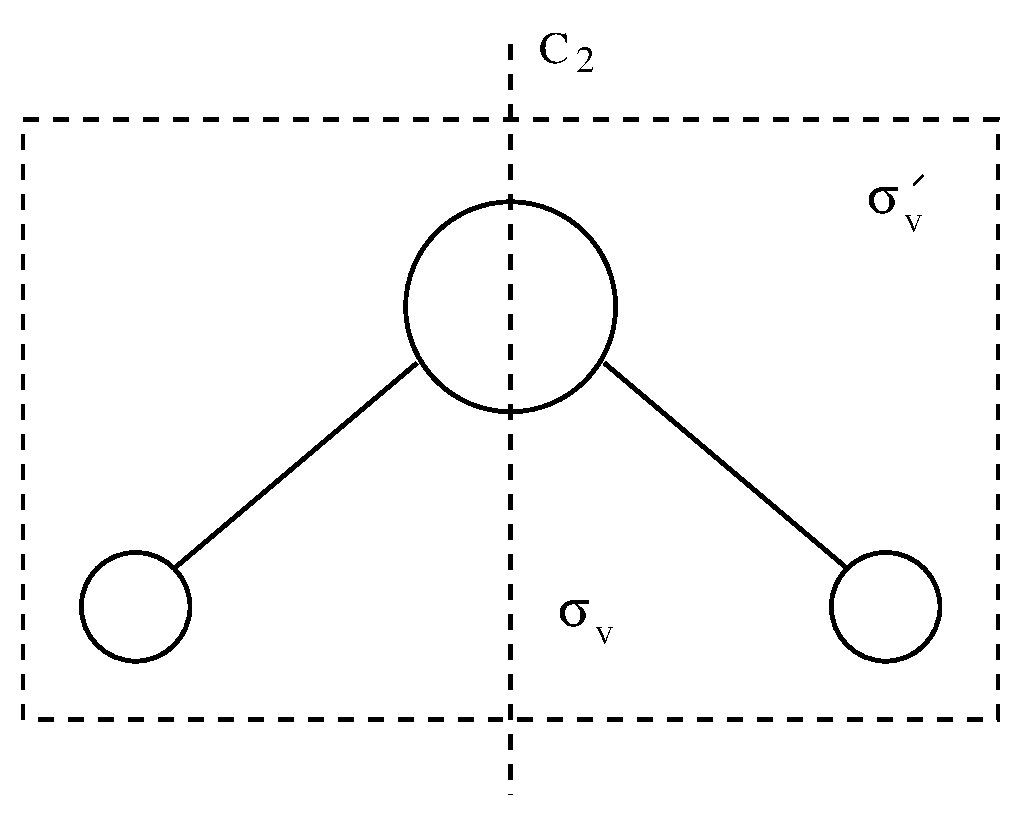
\epsfig{file={../fig/moleceau},width=6 cm,angle=-90}}   
 \caption{Mol\'ecule d'eau. Le groupe de sym\'etries $C_{2v}$
correspond \`a l'ensemble des op\'eartions : Identit\'e $E$, Rotation $C_2$
d'angle $\Pi$ autour de de l'axe vertical, sym\'etrie $\sigma_v$ par
rapport au plan perpendiculaire \`a la feuille et sym\'etrie
$\sigma'_v$ par rapport au plan de la feuille }
 \label{figmoleceau}
\end{figure}
Le groupe $C_{2v}$ est un des 32 groupes ponctuels
\cite{ma:group:Jones90,ph:solid:Ashcroft76}. La nomenclature est
explicit\'ee dans la figure \ref{figsymetr}.
\begin{figure}[htb]
\hspace{20mm}\input symetr.tex
 \caption{Nomenclature des groupes de sym\'etries en chimie. On teste
successivement la pr\'esence d'op\'erations de sym\'etrie en partant
du sommet de l'arbre. On parcourt l'arbre en fonction des r\'eponses
``o'', oui ou ``n'', non au test. $C_n$ d\'enote une rotation d'angle
$2\Pi/n$, $\sigma_h$ d\'enote une op\'eration de sym\'etrie par
rapport \`a un plan horizontal (perpendiculaire \`a l'axe de $C_n$),
$\sigma_h$ d\'enote une op\'eration de sym\'etrie par 
rapport \`a un plan vertical (passant par l'axe de $C_n$) et $i$,
l'inversion. Les noms des groupes sont encadr\'es.}
 \label{figsymetr}
\end{figure}
On peut caract\'eriser chacun de ces groupes par des tables de
caract\`eres qui d\'efinissent les repr\'esentations
irr\'eductibles\index{repr\'esentations irr\'eductibles} possibles de
ce groupe.  
La table de caract\`eres du groupe $C_{2v}$ est :
\begin{table}[hbt]\label{tabchar}
\caption{Table de caract\`ere du groupe $C_{2v}$.}
\begin{center}
\begin{tabular}{|l|r|r|r|r|}
$C_{2v}$ & $E$ & $C_2$ & $\sigma_v$ & $\sigma'_v$\\
\hline
$A_1$&1&1&1&1\\
$A_2$&1&1&-1&-1\\
$B_1$&1&-1&1&-1\\
$B_2$&1&-1&-1&1\\
\end{tabular}
\end{center}
\end{table}
Toutes les repr\'esentations du groupe $C_{2v}$ sont
unidimensionnelles. Elles sont au nombre de quatre et sont
d\'esign\'ees par $A_1$, $A_2$, $B_1$ et $B_2$. Dans le cas de la
mol\'ecule d'eau, l'espace est \`a neuf dimensions $e_i$
$i=1,\dots,9$. Les trois atomes 
sont en effet chacun rep\'er\'e par trois coordon\'ees. Une
repr\'esentation 
est ici le choix d'un vecteur $u$ combinaison lin\'eaire des
$e_{i}$ tel que pour tout \'el\'ement de sym\'etrie $g$ du groupe, on
ait :
\begin{equation}
g(u)=M_gu.
\end{equation}
La table de caract\`eres donne la trace, pour chaque $g$ de la matrice
$M_g$. Comme les repr\'esentations consid\'er\'ees ici sont
unidimensionelles, le caract\`ere est simplement la valeur propre
(unique) de $M_g$.
La figure \ref{figmodesmol} sh\'ematise les 9 repr\'esentations du
groupe $C_{2v}$ pour la mol\'ecule d'eau. On voit que l'espace des
$e_i$ se d\'ecompose en 9 sous-espaces invariants par les op\'erations
$g$. On \'ecrit que la repr\'esentation consid\'er\'ee $D$ se
d\'ecompose en la somme des rep\'esentations irr\'eductibles :
\begin{equation}
D=3A_1\oplus A_2\oplus2 B_1\oplus3 B_2.
\end{equation}
\begin{figure}
{\centering
\begin{tabular}[t]{ccc}

\epsffile{modesB2}
\epsffile{modesB2b}
\epsffile{modesB2bb}

\epsffile{modesB1}
\epsffile{modesB1b}
\epsffile{modesA2}

\epsffile{modesA1}
\epsffile{modesA1b}
\epsffile{modesA1bb}
\end{tabular} 
}
 \caption{Modes de la mol\'ecule $H_2O$. Les modes de vibration sont
encadr\'es. Les autres modes correspondent \`a des translations ou des
rotations.}
 \label{figmodesmol}
\end{figure}
En fait on voit que l'on a trois modes\index{mode} de translation, trois modes de
rotation. Les trois modes de vraie vibration sont encadr\'es dans la
figure \ref{figmodesmol}.
La dynamique est en g\'en\'eral d\'efinie par :
\begin{equation}
\frac{d^2x}{dt^2}=Mx
\end{equation}
o\`u $x$ est le vecteur d\'efinissant l'\'etat du syst\`eme dans la
base des $e_i$.
La dynamique est alors diagonalis\'ee dans le rep\`ere corespondant
aux trois modes de vibration : L'unique consid\'eration des sym\'etries
donne les vecteurs propres. Les valeurs
propres peuvent alors \^etre calcul\'ees bien plus rapidement. Ce
calcul n\'ecessite la connaissance des coefficients de $M$,
contrairement au calcul des vecteurs propres.

\subsection{Deux noyaux, un \'electron}
%%%%%%%%%%%%%%%%%
Ce cas correspond \`a l'\'etude de la mol\'ecule H$_2^+$
\cite{ph:mecaq:Rivail89,ph:mecaq:Cohen73}. 
Nous faisons l'approximation de Born-Oppenheimer, c'est \`a dire que
nous supposons les protons fixes. (Le mouvement des protons est lent
par rapport \`a celui des \'electrons.)
\begin{rem} Ce probl\`eme se r\'esout exactement. N\'eanmoins
illustrons sur cet exemple l'approximation variationnelle.
\end{rem}
Appliquons la m\'ethode LCAO (Linear Combination of Atomic Orbitals).
C'est \`a dire, supposons que la fonction d'onde d'un \'electron est une
combinaison lin\'eaire des fonctions d'onde des atomes \`a un
\'electrons : 
\begin{equation}
\psi=a\psi_1+b\psi_2
\end{equation}
Plus pr\'ecis\'ement choisissons comme fonctions les fonctions
$\phi_{s,1}$ et $\phi_{s,2}$ qui sont les orbitales $s$ centr\'ees sur
l'atome $1$ et $2$ respectivement.
Cette approximation sera d'autant plus vraie que R sera grand (voir
figure \ref{figH2plusS}).
\begin{figure}[htb]
 \centerline{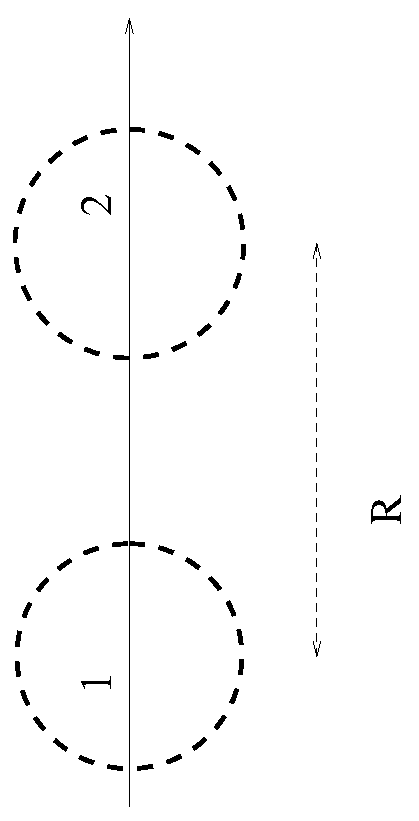
\epsfig{file={../fig/H2plusS},width=6 cm,angle=-90}}   
 \caption{Choix de la base des deux fonctions $1s$ associ\'ees \`a
chacun des atomes d'hydrog\`ene.}
 \label{figH2plusS}
\end{figure}
Les sym\'etries du probl\`emes nous am\`enent \`a \'ecrire :
\begin{eqnarray}
\psi_g&=&N_g(\psi_1+\psi_2)\\
\psi_u&=&N_u(\psi_1-\psi_2)
\end{eqnarray}
La notation avec les indices $g$ et $u$ est faite pour nous rappeler
la parit\'e des fonctions : $g$ pour {\it gerade}, pair en allemand, et
$u$ pour {\it ungerade} impair en allemand.La figure
\ref{figH2plusLCAO} repr\'esente ces deux fonctions.
\begin{figure}[htb]
\epsffile{H2plusLCAO}
\epsffile{H2plusLCAO2}
 \caption{Les fonctions $\psi_g$ et $\psi_u$ solutions du probl\`eme
d'approximation variationelle sur les deux orbitales $s$ des deux
atomes d'hydrog\`ene.}
 \label{figH2plusLCAO}
\end{figure}
La prise en compte de l'hamiltonien permet de montrer une lev\'ee de
d\'eg\'en\'erescence des \'energies comme le repr\'esente le diagramme
d'\'energie de la figure \ref{figH2plusLCAOener}.
\begin{figure}[htb]
 \centerline{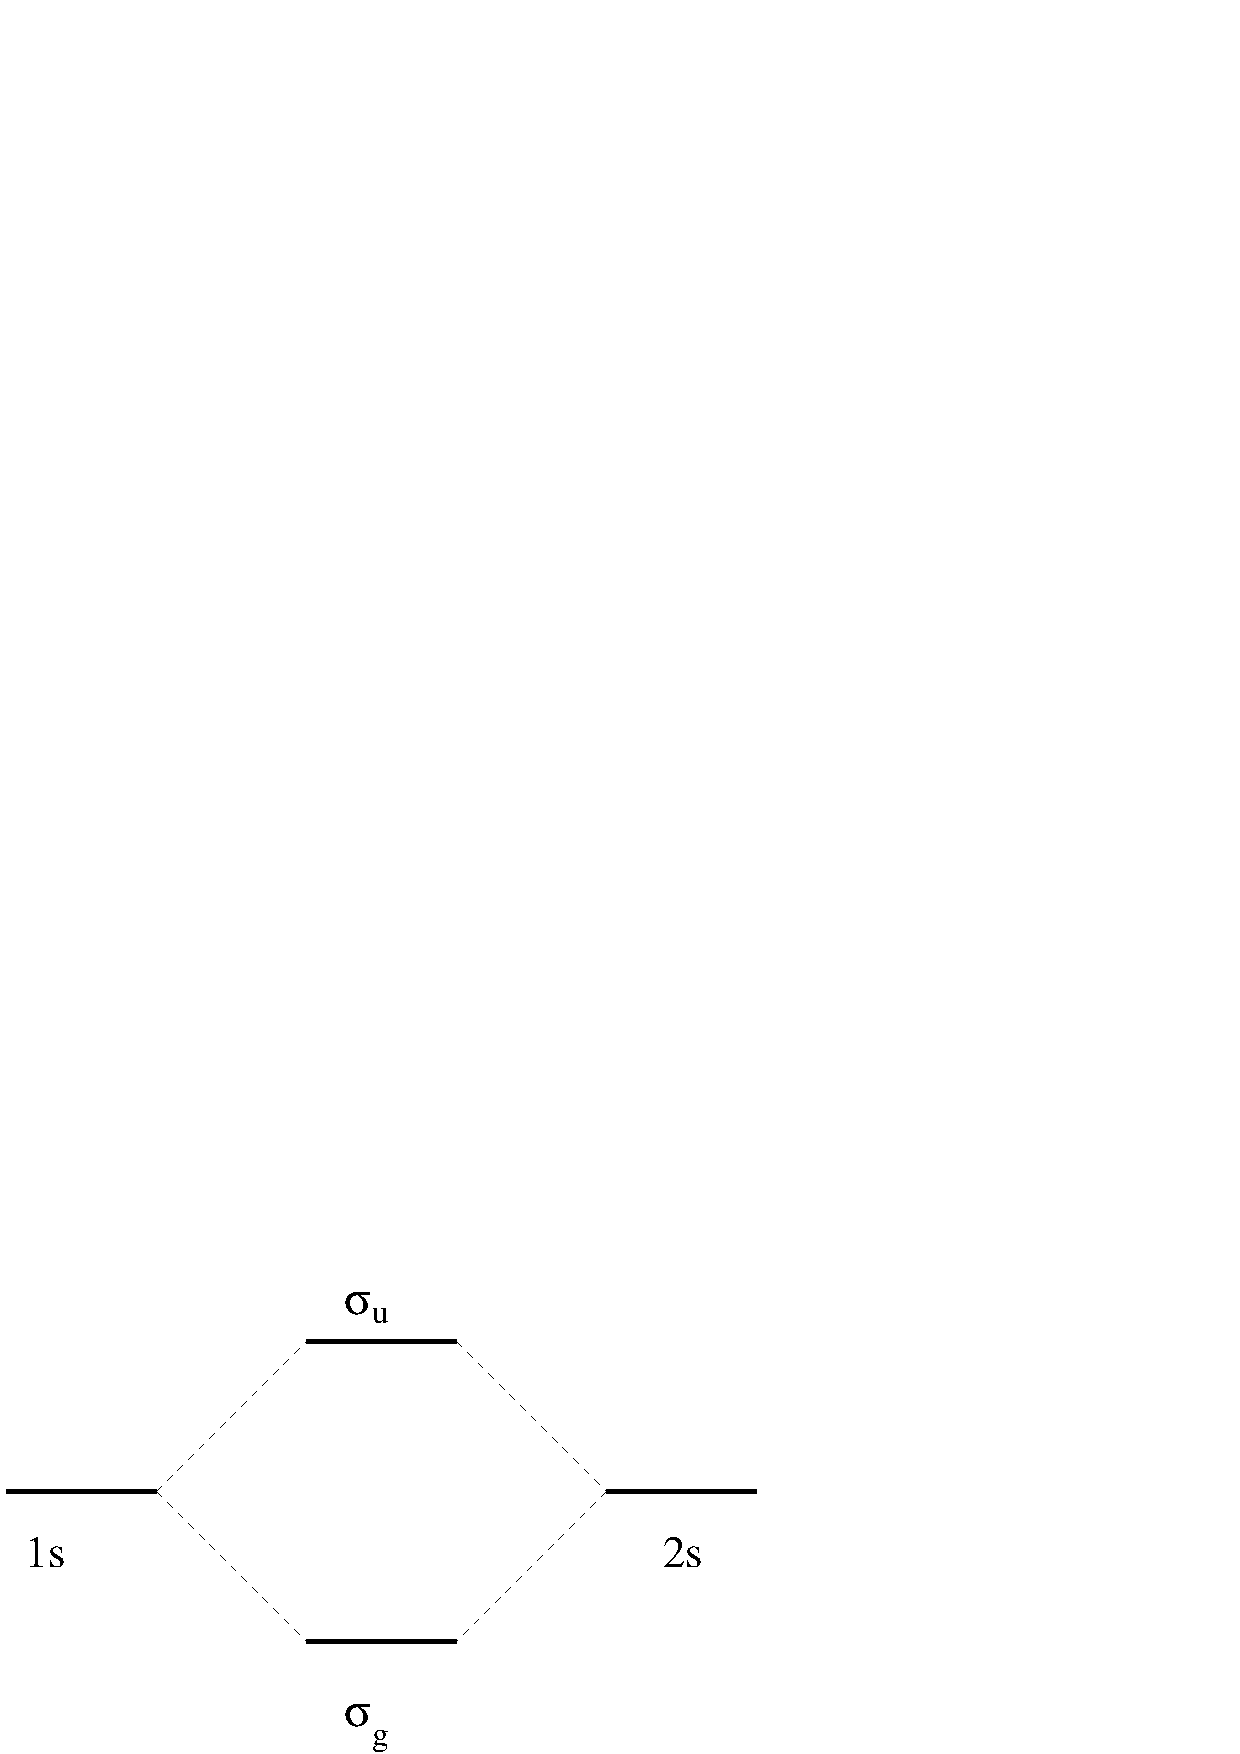
\epsfig{file={../fig/H2plusLCAOener},width=6 cm,angle=-90}}   
 \caption{Diagramme d'\'energie de la mol\'ecule $H_2^+$ par la
m\'ethode LCAO avec comme base de fonction les orbitales $s$ des deux
atomes d'hydrog\`ene.}
 \label{figH2plusLCAOener}
\end{figure}

\subsection{N noyaux, n \'electrons}\label{secnnne}
%%%%%%%%%%%%%%%%%
Dans ce cas, la consid\'eration des sym\'etries permet de trouver des
sous-espaces propres. Ces consid\'erations sont li\'ees \`a la
th\'eorie de la repr\'esentation des groupes ponctuels.
Lorsque les atomes d'une mol\'ecule sont situ\'es dans un m\^eme plan,
celui-ci est \'el\'ement de sym\'etrie. Dans le cas d'une mol\'ecule
lin\'eaire, le plan passant par l'axe de la mol\'ecule est aussi un
plan de sym\'etrie. On distingue deux types
d'orbitales : 
\begin{defn}
Les orbitales $\sigma$ sont celles qui se conservent dans la r\'eflexion
par rapport au plan.
\end{defn}
\begin{defn}
Les orbitales $\pi$ sont celles qui changent de signe dans la r\'eflexion
par rapport au plan.
\end{defn}
Envisageons le cas d'une mol\'ecule lin\'eaire. Pour
d'autres exemples, on se reportera \`a \cite{ph:mecaq:Rivail89}.
\begin{exmp}
{\bf mol\'ecule BeH$_2$}.
Nous cherchons notre fonction d'onde dans l'espace engendr\'e par
les orbitales $2s$ et $z$ de l'atome de berylium Be et par les deux
orbitales $1s$ des deux atomes d'hydrog\`ene. L'espace est donc \`a quatre
dimensions (on a laiss\'e de c\^ot\'e les orbitales $x$ et $y$) et
l'hamiltonien \`a diagonaliser dans cette base s'\'ecrit en
g\'en\'eral comme une matrice $4\times 4$.
La prise en compte des sym\'etries permet de mettre cette matrice sous
forme {\it diagonale par blocs}.
Nous choisissons comme base :
\{$2s,z,1s_1+1s_2,1s_1-1s_2$\}. Alors les orbitales s'\'ecrivent :
\begin{eqnarray}
\sigma_s&=&\alpha_12s+\beta_1(1s_1+1s_2)\\
\sigma_s^*&=&\alpha_22s-\beta_2(1s_1+1s_2)\\
\sigma_p&=&\alpha_3z+\beta_3(1s_1-1s_2)\\
\sigma_p^*&=&\alpha_4z-\beta_4(1s_1-1s_2)
\end{eqnarray}
Ces liaisons sont d\'elocalis\'ees sur trois atomes et sont
sch\'ematis\'ees dans la figure \ref{figBeH2orb}.
\begin{figure}[htb]
 \centerline{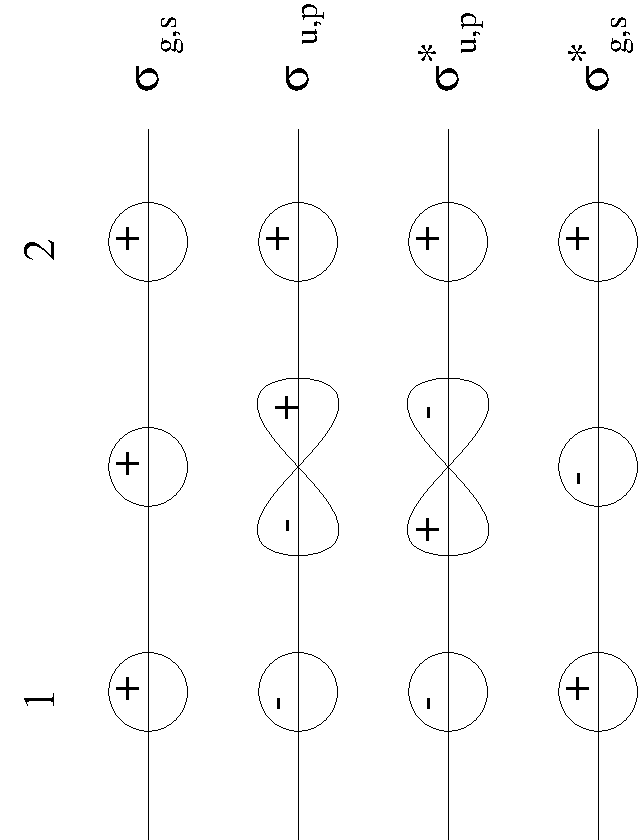
\epsfig{file={../fig/BeH2orb},width=6 cm,angle=-90}}   
 \caption{Diagramme d'\'energie de la mol\'ecule $H_2^+$ par la
m\'ethode LCAO avec comme base de fonction les orbitales $s$ des deux
atomes d'hydrog\`ene.}
 \label{figBeH2orb}
\end{figure}
Nous avons deux orbitales liantes et deux antiliantes. Le diagramme
d'\'energie est repr\'esent\'e dans la figure \ref{figBeH2ene}. Les quatre
\'electrons occupent les deux orbitales liantes, dans l'etat
fondamental. 
\begin{figure}[htb]
 \centerline{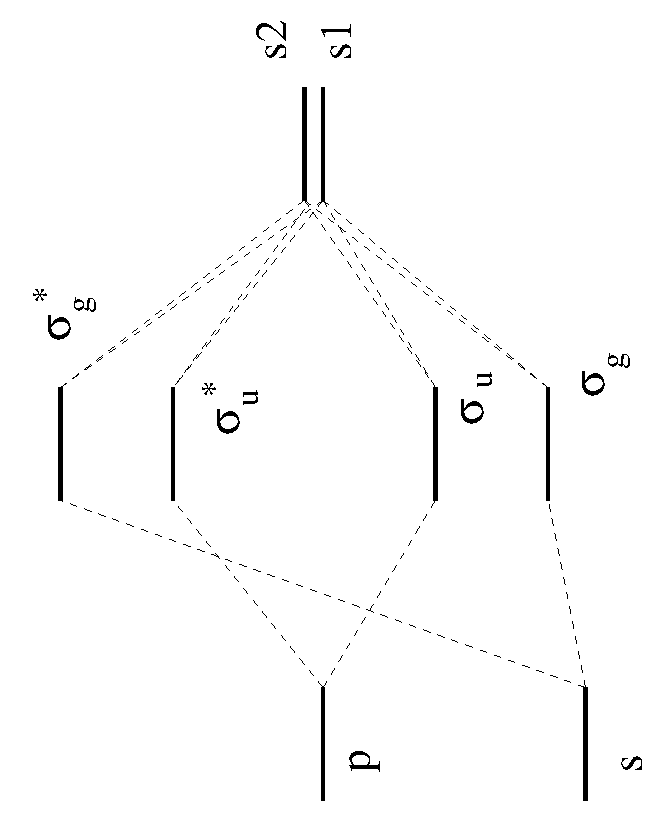
\epsfig{file={../fig/BeH2ene},width=6 cm,angle=-90}}   
 \caption{Diagramme d'\'energie de la mol\'ecule $H_2^+$ par la
m\'ethode LCAO avec comme base de fonction les orbitales $s$ des deux
atomes d'hydrog\`ene.}
 \label{figBeH2ene}
\end{figure}
\end{exmp}
L'\'etude exp\'erimentale des mol\'ecules montre que les
caract\'eristiques d'une liaison d\'ependent peu de la nature des autres
atomes. (\cite{ph:chimi:Didier}) Nous simplifions donc le probl\`eme en
consid\'erant des orbitales mol\'eculaires $\sigma$ dicentriques,
c'est-\`a-dire localis\'ees entre deux atomes. Ces orbitales sont
dites hybrides.
\begin{exmp}
Reprenons l'exemple de la mol\'ecule BeH$_2$. La mol\'ecule est
lin\'eaire. Cette g\'eom\'etrie est bien d\'ecrite par l'hybridation
$s-p$. On d\'efinit les orbitales hybrides :
\begin{eqnarray}
d_1&=&\frac{1}{\sqrt{2}}(s+z)\\
d_2&=&\frac{1}{\sqrt{2}}(s-z)
\end{eqnarray}
Au lieu de consid\'erer la base \{$2s,z,1s_1,1s_2$\}, on consid\`ere
d\`es le d\'epart la base
\{$d_1,d_2,1s_1,1s_2$\}.
\end {exmp}
\section{Le solide}\label{secsolidmq}
%%%%%%%%%%%%%%%%%%%%%%%%%%%%%%
\subsection{Th\'eor\`eme de Bloch}\label{sectheobloch}
%%%%%%%%%%%%%%%
Consid\'erons le probl\`eme spectral suivant :
\begin{prob}
Trouver $\psi(r)$ et $\epsilon$ tels que
\begin{equation}
[-\frac{\hbar^2}{2m}\nabla^2+V(r)]\psi(r)=\epsilon\psi(r)
\end{equation}
o\`u $V(r)$ est une fonction p\'eriodique
\end{prob}
Le th\'eor\`eme de
Bloch\cite{ma:equad:Dautray5,ph:solid:Kittel67,ph:physt:Diu89}
permet\index{Bloch (th\'eor\`eme de)} de chercher les fonctions
propres sous 
une forme qui utilise les sym\'etries du probl\`eme. 
\begin{thm}\label{theobloch}{\bf Th\'eor\`eme de Bloch --} Si $V(r)$
est p\'eriodique alors 
la fonction d'onde $\psi$ solution du probl\`eme spectral peut
s'\'ecrire : 
\begin{equation}
\psi(r)=\psi_k(r)=e^{ikr}u_k(r)
\end{equation}
avec $ u_k(r)=U_k(r+R)$ (la fonction $u_k$ a la p\'eriodicit\'e du
r\'eseau).  
\end{thm}
\begin{pf}
L'op\'erateur $-\frac{\hbar^2}{2m}\nabla^2+V(r)$ commute avec les
translations $\tau_j$ d\'efinies par $\tau_a\psi(r)=\psi(r+a)$.
Les fonctions propres de $\tau_a$ sont telles que :
\begin{equation}
\tau_a\psi=\psi
\label{tra}
\end{equation}
Montrons comment les propri\'et\'es de la transform\'ee de
Fourier\index{Fourier} 
nous donnent
les valeurs propres. En effet l'\'equation \ref{tra} s'\'ecrit :
\begin{equation}
\delta(x-a)*\psi(r)=\psi(r)
\end{equation}
Par transformation de Fourier on obtient
\begin{equation}
e^{-2i\pi ka}\hat{\psi}=\hat{\psi}
\end{equation}
ce qui donne $k_n=n/a$ et la valeur propre
$\lambda=e^{-2i\pi k_na}$.\footnote{%%%%%%%%%%%%%
Ainsi chaque repr\'esentation irr\'eductible\index{repr\'esentation irr\'eductible} du groupe des translations
est caract\'eris\'ee par un vecteur $k$. Nous d\'esignons cette
repr\'esentation par $\Gamma_k$.}%%%%%%%%%%%%%%%
Par ailleurs, la focntion propre peut toujours \^etre \'ecrite sous la forme :
\begin{equation}
\psi_k(r)=e^{ikr}u_k(r)
\end{equation}
On montre enfin que $u_k$ est p\'eriodique\footnote{%%%%%
En effet, \'ecrivons de deux mani\`eres l'action de $\tau_a$ :
\begin{equation}
\tau_a\psi_k=e^{ika}\psi_k
\end{equation}
et
\begin{equation}
\tau_a\psi_k=e^{ik(r+a)u_k(r+a)}
\end{equation}
}%%%%%%%%%%%%%%%%%%%%%
\end{pf}
\subsection{\'Electron libre}
%%%%%%%%%%%%%%%%%%%%%%%%%%%%%
L'hamiltonien s'\'ecrit\cite{ph:solid:Kittel67,ph:solid:Callaway64}
ici : 
\begin{equation}
H=-\frac{\hbar^2}{2m}\nabla^2+V(r)
\end{equation}
o\`u $V(r)$ est le potentiel d'une bo\^\i te p\'eriodique de p\'eriode $a$
(voir la figure \ref{figpotperioboit})
\ref{figeneeleclib}. 
\begin{figure}[htb]
 \centerline{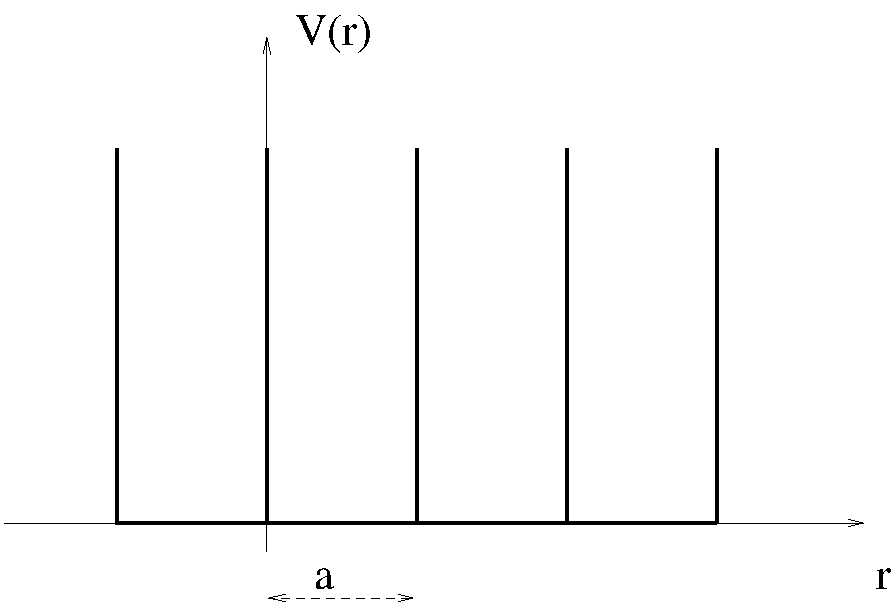
\epsfig{file={../fig/potperioboit},width=6 cm,angle=-90}}   
 \caption{Potentiel dans l'approximation de l'\'electron libre.}
 \label{figpotperioboit}
\end{figure}
Les fonctions propres de $H$ sont les fonctions propres de $\nabla^2$
(invariance par translation) qui v\'erifient les conditions aux bords.
Le th\'eor\`eme de Bloch implique que $\phi$ est de la forme :
\begin{equation}
\psi_k=e^{ikr}u_k(\bar{r})
\end{equation}
o\`u  $u_k(\bar{r})$ est une fonction qui poss\`ede la sym\'etrie du
cristal\index{cristal}, c'est-\`a-dire qui est invariante par
translation : 
\begin{equation}
u_k(\bar{r}+\bar{R}_i)=u_k(\bar{r})
\end{equation}

Ici (\cite{ph:solid:Callaway64}), on peut donc prendre pour $u_k$
toute fonction de la forme :
\begin{equation}
u_k(\bar{r})=e^{iK_nr}
\end{equation}
En portant cette fonction dans l'\'equation de Scr\"odinger, on obtient
l'\'energie suivante : 
\begin{equation}
E_k=\frac{\hbar^2}{2m}|k+K_n|^2
\end{equation}
o\`u $K_n$ prend les valeurs $\frac{2n\pi}{a}$, o\`u $a$ est la
p\'eriodicit\'e du r\'eseau et $n$ un entier.
Le graphe de $E$ en fonction de $k$ est repr\'esent\'e dans la figure
\ref{figeneeleclib}. 
\begin{figure}[htb]
 \centerline{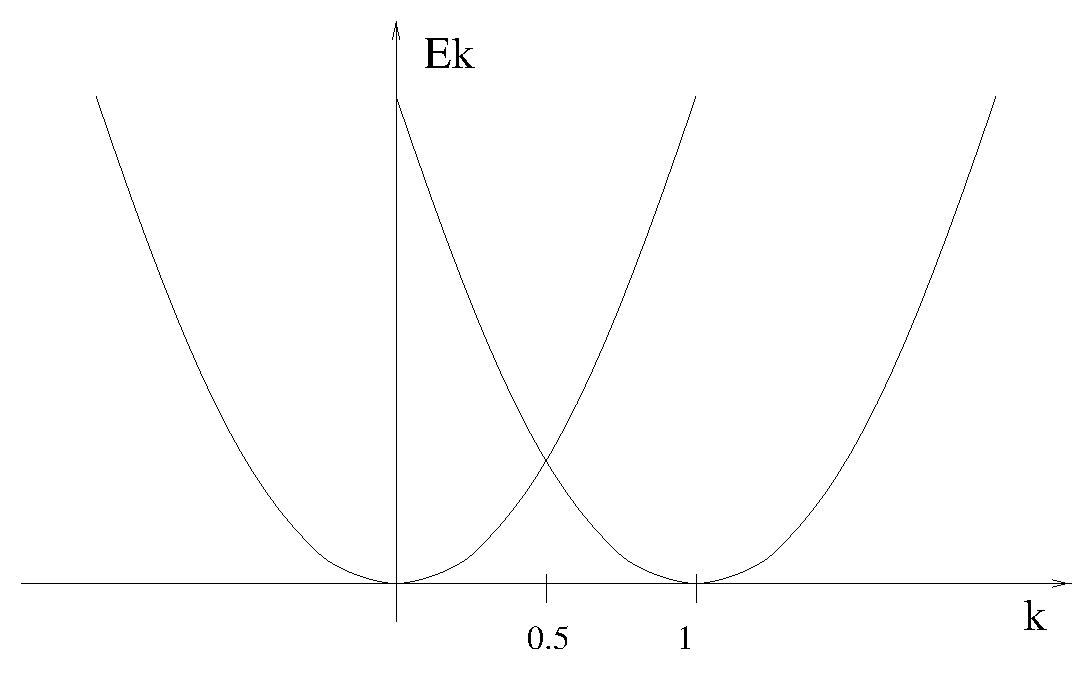
\epsfig{file={../fig/eneeleclib},width=6 cm,angle=-90}}   
 \caption{\'Energie d'un mode $k$ dans l'approximation de l'\'electron
libre (\'electron dans une bo\^\i te).}
 \label{figeneeleclib}
\end{figure}

\subsection{\'Electron quasi-libre}
%%%%%%%%%%%%%%%%%%%%%%%%%%%%%
Montrons que si le potentiel n'est plus celui d'une bo\^\i te p\'eriodique,
la d\'eg\'en\'erescence en $k=\frac{K_1}{2}$ est lev\'ee.
Donnons--nous par exemple un potentiel de la forme :
\begin{equation}
V(x)=V_{boite}+\epsilon e^{iK_1r}
\end{equation}
Dans le mod\`ele de l'\'electron libre, les deux fonctions propres 
\begin{eqnarray}
\psi_{1k}&=&e^{ikr}\\
\psi_{2k}&=&e^{ikr}e^{iK_1r}
\end{eqnarray}
sont d\'eg\`en\'er\'ees. La diagonalisation de l'hamiltonien dans
cette base permet de montrer que la d\'eg\'en\'erescence est lev\'ee
par la perturbation.
\subsection{Liaison forte}
%%%%%%%%%%%%%%%%%%%%%%%%%%%
L'approximation de la liaison forte
(tight-binding)\cite{ph:solid:Ashcroft76}  consiste \`a
approcher l'espace des \'etats par l'espace engendr\'e par les
orbitales atomiques centr\'ees au noeud du r\'eseau :
\begin{equation}
\psi(r)=\sum_j c_j\phi_{at}(r-R_j)
\end{equation}
Le th\'eor\`eme de Bloch am\`ene \`a chercher $\psi_k$ sous la forme :
\begin{equation}
\psi_k(r)=e^{ikr}u_k(r)
\end{equation}
En identifiant $u_k(r)$ et $u_k(r+R_i)$ on montre que $c_l=e^{ikK_l}$.
Une fois encore, la consid\'eration des sym\'etries d\'etermine
compl\`etement les vecteurs propres. Les \'energies sont calcul\'ees
gr\^ace \`a l'expression du hamiltonien. Nous renvoyons \`a
\cite{ph:solid:Ashcroft76} pour plus de d\'etails. 


\section{Exercices}
%%%%%%%%%%%%%%%%%%%

\begin{exo}
Nommer le groupe de sym\'etrie auquel appartient la mol\'ecule $NH_{3}$.
\end{exo}
\begin{exo}
Param\'etriser les vibrations d'une mol\'ecule $NH_{3}$ et d\'ecomposer en
l'une 
de repr\'esentations irr\'eductibles la repr\'esentation associ\'ee \`a la
param\'etrisation que vous proposez. 
\end{exo}

\begin{exo}
Proposez une autre base pour l'\'etude de la mol\'ecule $BeH_{2}$ que celles
donn\'ees \`a la section \ref{secnnne}.
\end{exo}
\begin{exo}
Trouver les \'etats propres ainsi que les \'energies d'un \'electron dans une
boite carr\'ee de c\^ot\'e $a$ (potentiel nul pour $-a/2<x<a/2$ et
$-a/2<y<+a/2$, potentiel infini ailleurs). 
Que se passe t-il si au potentiel de la bo\^\i te on ajoute un perturbation
constante de valeur $\epsilon$ sur un quart de la surface de la boite
($0<y<a/2$ et $0<y<a/2$).
Calculer par perturbation les nouvelles \'energies et les nouveaux vecteur
propres. Des consid\'erations de sym\'etrie auraient--elles permis de pr\'evoir
les vecteurs propres ?
\end{exo}



\chapter{Physique  statistique}\label{chapphysstat}
%%%%%%%%%%%%%%%%%%%%%%%%%%%%
\section{Introduction}
%%%%%%%%%%%%%%%%%%%%%
La physique statistique cherche \`a rendre compte des propri\'et\'es
de la mati\`ere \`a l'\'echelle macroscopique, en partant d'une
description microscopique (atomes, mol\'ecules, etc\dots). Le tr\`es
grand nombre de particules constituant un syst\`eme macroscopique
justifie une description probabiliste du syst\`eme. La m\'ecanique
quantique (voir le chapitre \ref{chapmq}) permet de d\'ecrire en
partie les syst\`emes constitu\'es 
d'un grand nombre de particules : L'\'equation de
Schr\"odinger fournit les diff\'erents \'etats possibles ainsi que
l'\'energie qui leur est associ\'ee. La physique statistique permet de
calculer des probabilit\'es d'occupation $P_l$ d'un 
\'etat $l$. Elle introduit les concepts
fondamentaux de temp\'erature, de chaleur\dots

L'obtention de la probabilit\'e $P_l$ se fait par un principe
fondamental qui consiste \`a dire que le syst\`eme tend \`a se mettre
dans un \'etat de d\'esordre maximum\cite{ph:physt:Reif64,ph:physt:Diu89}. Un mesure du
d\'esordre est 
donn\'ee par l'entropie statistique \footnote{Cette formule est
analogue de la d\'efinition de l'entropie d'information choisis par Shannon\cite{ph:physt:Shannon49}.}\index{entropie}
\begin{equation}
S=-k_B\sum P_l \ln P_l
\end{equation}
Le principe s'\'ennonce donc :
\begin{postulat}
\`A l'\'equilibre macroscopique, la distribution statistique des
\'etats microscopiques est, parmi toutes celles qui v\'erifient les
contraintes ext\'erieures impos\'ees au syst\`eme, celle qui rend
l'entropie statistique maximum.
\end{postulat}
\begin{rem}
Ce probl\`eme correspond \`a un classique probl\`eme de
maximisation (voir le chapitre \ref{chapmetvar}) qui peut \^etre
trait\'e en particulier par des 
m\'ethodes de multiplicateurs de Lagrange\index{Lagrange
(multiplicateurs de)} comme nous allons le voir.
\end{rem}
\section{Maximalisation de l'entropie}\label{secmaxient}
%%%%%%%%%%%%%%%%%%%%%%%%%%%%%%%%%%%%%%%%%%%
Nous pr\'ecisons ici le probl\`eme math\'ematique associ\'e au calcul
de probabilit\'es $P_l$ :\index{maximalisation}
En g\'en\'eral, le syst\`eme est d\'ecrit par deux types de
variables. Des variables externes $y^i$ dont la valeur est fix\'ee \`a
$y_j$ par l'ext\'erieur du syst\`eme et des variables internes $X^i$
dont seule la moyenne est fix\'ee.
Le probl\`eme \`a r\'esoudre est donc le suivant : 
\begin{prob}
Trouver la distribution de probabilit\'e $P_l$ sur les \'etats $(l)$ du
syst\`eme qui maximise l'entropie
\begin{equation}
S=-k_B\sum P_l \ln (P_l)
\end{equation}
et qui v\'erifie les contraintes suivantes :
\begin{eqnarray}
\sum X_{l}^iP_l&=&\bar{X^i}\\
\sum P_l&=&1
\end{eqnarray}
\end{prob}
La maximisation de la fonctionnelle entropie par la technique des
multiplicateurs de Lagrange donne :
\begin{equation}
P_l=\frac{1}{Z}e^{-\lambda_1 X^{1}_l-\lambda_2 X^{2}_l- ...}
\end{equation}
o\`u  la fonction $Z$, appel\'ee fonction de partition,
\index{fonction de partition} est d\'efinie par :
\begin{equation}
Z=\sum_{(l)} e^{-\lambda_1 X^{1}_l-\lambda_2 X^{2}_l- ...}
\end{equation}
Les nombres $\lambda_i$ sont les multiplicateurs de Lagrange.
\begin{exmp}
Dans le cas o\`u c'est l'\'energie moyenne qui est fix\'ee, le
multiplicateur de Lagrange est :
\begin{equation}
\lambda=\frac{1}{k_BT}
\end{equation}
o\`u $T$ est la temp\'erature.\index{temp\'erature} Il s'agit donc
d'une d\'efinition 
math\'ematique de la temp\'erature.
\end{exmp}
\begin{exmp}
Dans le cas o\`u c'est le nombre moyen de particules qui est fix\'e, le
multiplicateur de Lagrange est not\'e $\mu$ et est appel\'e potentiel
chimique du syst\`eme.
\end{exmp}
Les relations sur les moyennes destin\'ees en principe \`a la
d\'etermination des param\`etres $\lambda_i$ \`a partir des moyennes
$\bar{X_i}$ peuvent \^etre \'ecrites sous la forme :
\begin{equation}
-\frac{\partial}{\partial \lambda_i}\ln Z(y,\lambda_1,\lambda_2,...) =
\bar{X_i} 
\end{equation}
On d\'efinit $L$ par :
\begin{equation}
L=\ln Z(y,\lambda_1,\lambda_2,...)
\end{equation}
On peut montrer\footnote{Par d\'efinition
\begin{equation}
S=-k_B\sum P_l \ln (P_l)
\end{equation}
D'o\`u
\begin{equation}
S/k=-\sum P_l\ln(\frac{1}{Z}e^{-\lambda_1 X^{1}_l-\lambda_2 X^{2}_l- ...})
\end{equation}
\begin{equation}
S/k=1\ln Z+\lambda_1 \bar{X^{1}_l}+\lambda_2 \bar{X^{2}_l}+ ...
\end{equation}
} que :
\begin{equation}
S/k=\sum \lambda_i \bar{X^i}+\ln(Z)
\end{equation}
La relation qui permet de passer de $L$ \`a $S$ est appel\'ee {\bf
transformation de Legendre}.\index{Legendre (transformation de)}
$L$ est une fonction des $y^i$ et $\lambda_j$, $S$ est une fonction
des $ y^i$ et des $\bar{X^j}$.
\section{Distribution canonique en m\'ecanique
classique}\label{secdistclassi} 
%%%%%%%%%%%%%%%%%%%%%%%%%%%%%%%%%%%%%%%%%%%%%%%%%%%%%%%%%%
Consid\'erons un syst\`eme dont seule l'\'energie moyenne est fix\'ee.
La probabilit\'e pour que le syst\`eme se trouve dans l'\'etat
quantique $(l)$ d'\'energie $E_l$ est donn\'ee par (voir section
pr\'ec\'edente) :
\begin{equation}
P_l=\frac{1}{Z}e^{-E_l/k_BT}
\end{equation}
Consid\'erons une description classique de ce m\^eme syst\`eme. Par
exemple si le syst\`eme est un ensemble de $N$ particules dont la
position 
est l'impulsion sont not\'ees $q_i$ et $p_i$, alors ce syst\`eme est
d\'ecrit par un hamiltonien classique $H(q_i,p_i)$.
On d\'efinit donc une densit\'e de probabilit\'e classique par
\begin{equation}\label{eqdensiprobaclas}
w^c(q_i,p_i)=\frac{1}{A}e^{-H(q_i,p_i)/k_BT}
\end{equation}
La grandeur $w^c(q_i,p_i)dq_idr_i$ repr\'esente la probabilit\'e pour
que le syst\`eme soit dans la partie de l'espace des phases compris
entre $q_i,p_i$ et $q_i+dq_i, p_i+dp_i$.
Les coefficients de normation $Z$ et $A$ sont proportionnels.
\begin{equation}
A=\int dq_1...dq_n\int dp_1...dp_n e^{-H(q_i,p_i)/k_BT}
\end{equation}
On montre \cite{ph:physt:Diu89} la relation
\begin{equation}
Z=\frac{1}{(2\pi\hbar)^{3N}}A
\end{equation}
$2\pi\hbar^N$ est en quelque sorte le volume de l'espace des phases
\'equivalent \`a un \'etat quantique.
\begin{rem}
On remarque que cette
valeur correspond \`a la pr\'ecision minimale que l'on peut avoir sur
le volume de l'espace des phases d'apr\`es le principe d'incertitude
d'Heisenberg:\index{Heisenberg (principe d'incertitude d')}
\begin{equation}
\Delta x \Delta p > \hbar
\end{equation}
\end{rem}
La fonction de partition donn\'ee par une approche classique devient
donc :
\begin{equation}
Z=\frac{1}{(2\pi\hbar)^N}\int dq_1...dq_n\int dp_1...dp_n e^{-H(q_i,p_i)/k_BT}
\end{equation}
Mais cette technique de passage de la description quantique \`a la
description classique pose certains probl\`emes de compatibilit\'e. Par
exemple, en m\'ecanique quantique existe un postulat permettant de
traiter le cas d'un ensemble de particules identiques. L'application
brute de la formule \ref{eqdensiprobaclas} aboutit \`a des r\'esultats
erron\'es (paradoxe de Gibbs). On doit donc dans le traitement
classique ajouter un postulat pour la description classique d'un
syst\`eme constitu\'e de particules identiques :
\begin{postulat}
On ne compte pas comme distincts deux \'etats du syst\`eme qui ne
diff\'erent que par permutation
\end{postulat}
Ce qui donne pour la fonction de partition classique pour un syst\`eme
de $N$ particules identiques :
\begin{equation}
Z=\frac{1}{N!}\frac{1}{(2\pi\hbar)^{3N}}\int\prod dp^{3}_i dq^{3}_i
e^{-H(q_i,p_i)/k_BT} 
\end{equation}

\section{Rel\^achement de contrainte}\label{secrelacont}
%%%%%%%
Nous avons d\'efini \`a la section \ref{secmaxient} les variables
externes, fix\'ees par l'ext\'erieur, et les variables internes libres
de fluctuer. Consid\'erons un syst\`eme $L$ poss\'edant des $N+N'$
variables \index{contrainte}
internes $n_1,\dots,n_N,X_1,\dots,X_{N'}$. Ce syst\`eme poss\`ede une
fonction de partition $Z^{L}$. Consid\'erons maintenant le
syst\`eme $F$, pour lequel les variables $n_i$ sont cette fois
consid\'er\'ees comme des variables externes ayant pour valeur $N_i$.
Ce syst\`eme $F$ poss\`ede une autre fonction de partition 
$Z^{F}$. Le syst\`eme $L$ s'obtient \`a partir du syst\`eme $F$ par
un rel\^achement de contrainte\cite{ph:physt:Boccara76}. Voici un
th\'eor\`eme qui relie les valeurs les  plus 
probables des variables internes $n_i$ dans les syst\`eme $L$ \`a la
fonction de partition $Z^F$ du syst\`eme $F$ :
\begin{thm}
Les valeurs $n_i$ les plus probables dans un syst\`eme $L$ o\`u les
$n_i$ sont 
libres de fluctuer, sont les $n_i$ qui annulent la diff\'erentielle de la
fonction de partition $Z^{F}$ o\`u les $n_i$ sont fixes. 
\end{thm}
\begin{pf}
Consid\'erons la description o\`u les $n_i$ sont libres. La probabilit\'e
pour que $n_1=N_1$,$\cdots$,$n_N=N_N$ est :
\begin{equation}
P(n_1=N_1,\cdots,n_N=N_N)=\sum_{(l)/n_1=N_1,\cdots,n_N=N_N}P^{L}_l
\end{equation}
Soit
\begin{eqnarray}
\lefteqn{P(n_1=N_1,\cdots,n_N=N_N) = }\\
&&\frac{1}{Z^{nl}} e^
{-\lambda_{n_1}N_1-\cdots-\lambda_{n_N}N_N} \sum_{(l)/n_1 =
N_1,\cdots,n_N=N_N} e^ {-\lambda_{X_1}\bar X_1-\lambda_{X_2}\bar X_2} 
\end{eqnarray}
Les valeurs les plus probables annulent la diff\'erentielle :
\begin{equation}
dP(n_1=N_1,\cdots,n_N=N_N) = 0
\end{equation}
Soit
\begin{equation}
d\log(Z^{F})=\sum_i \frac{\partial \log(Z^{F})}{\partial n_i}dn_i=0
\end{equation}
\end{pf}
%%%%%%%%%%%
\begin{rem}
Cette relation est utilis\'ee en chimie : elle constitue la relation
fondementale de la r\'eaction chimique. Dans ce cas les $N$ variables
$n_i$ 
repr\'esentent les nombres de particules des $N$ esp\`eces $i$ et $N'=2$
avec $X_1=E$ et $X_2=V$. L'\'equation de la r\'eaction chimique donne
des liaisons sur les variables 
$n_i$ par les coefficients stoechiom\'etriques.
\end{rem}
\'Ecrivons une relation de type Gibbs-Duheim \index{Gibbs-Duheim
(relation de)}:
\begin{equation}
S^{F}/k=\lambda_{X_1}\bar X_1+\lambda_{X_2}\bar X_2+\ln (Z^{F})
\end{equation}
\begin{equation}
S^{L}/k=\lambda_{X_1}\bar X_1+\lambda_{X_2}\bar X_2+\lambda_{n_1}\bar{n_1}+\cdots+\ln (Z^{L})
\end{equation}
\`A l'\'equilibre thermodynamique $S^{F}=S^{L}$ donc :
\begin{equation}
\lambda_{n_i}=\frac{\partial \ln (Z^{F})}{\partial n_i}
\end{equation}
\begin{exmp}
Cette derni\`ere \'egalit\'e fournit un moyen de calculer le potentiel
chimique d'un syst\`eme.\index{potentiel chimique}
\begin{equation}
\mu_i=\frac{\partial \ln (Z^{F})}{\partial n_i}
\end{equation}
On note en g\'en\'eral $-\ln(Z^{F})=G$.
\end{exmp}
\begin{exmp}
Consid\'erons le cas o\`u les variables $n_i$ sont les nombres de
particules de l'esp\`ece $i$.
Si les particules sont ind\'ependantes, l'\'energie associ\'ee \`a un
\'etat d\'ecrivant les $N$ particules (l'ensemble des particules de type $i$
\'etant dans un \'etat $l_i$) est la somme des $N$ \'energies associ\'ees aux
\'etats $l_i$ et donc :
\begin{equation}
\ln Z^F(\lambda_{X_1},\lambda_{X_2},n_1,n_2)=\ln
Z^F_1(\lambda_{X_1},\lambda_{X_2},n_1)+\dots+\ln
Z^F_N(\lambda_{X_1},\lambda_{X_2},n_N) 
\end{equation}
o\`u $Z^F_i(\lambda_{X_1},\lambda_{X_2},n_i)$ repr\'esente la fonction
de partition du syst\`eme constitu\'e uniquement de particules de type
$i$, pour lequel la valeur de la variable $n_i$ est fix\'ee. 
On a donc :
\begin{equation}
\frac{\partial \ln Z^F_1}{\partial n_1} dn_1+\dots+\frac{\partial \ln
Z^F_N}{\partial n_N} dn_N=0 
\end{equation}
\end{exmp}
\begin{rem}
Si on pose $\lambda_1=\beta$,$\lambda_2=\beta p$ et $\lambda_{n_1}=-\beta\mu$ avec $G=-k_BT\ln Z^{nf}$ on a $G(T,p,n)=E+pV-TS$ et $G'(T,p,\mu)=E+pV-TS-\mu-{n_1}$, ce qui est la relation de Gibbs-Duheim.
\end{rem}
\begin{exmp}
Nous proposons dans cette exemple de d\'emontrer la formule de
Nernst\index{formule de Nernst}
d\'ecrivant une r\'eaction
d'oxydo-r\'eduction.\index{oxydo-r\'eduction} Ce type de r\'eaction 
chimique peut \^etre abord\'e par le formalisme pr\'ec\'edent. Nous
allons pr\'eciser les notations dans ce cas particulier.

La d\'emonstration de la formule de Nernst que nous allons pr\'esenter est
diff\'erente de celle pr\'esent\'ee classiquement dans les manuels de
chimie. Les \'electrons subissent une variation d'\'energie potentielle en
passant du potentiel de la solution au potentiel du m\'etal.
Cette variation d'\'energie potentielle peut-\^etre consid\'er\'ee
comme le 
travail re\c cu par le syst\`eme ou comme la variation d'\'energie
interne du 
syst\`eme, selon que l'on consid\`ere comme syst\`eme les \'electrons
ou bien 
l'ensemble de la solution, du m\'etal et des \'electrons. Nous adoptons le
deuxi\`eme point de vue.
Consid\'erons la fonction enthalpie libre $ G(T,p,n_i,E_p)$. Les
variables $n_i$ et $E_p$ sont libres de fluctuer. Elles vont prendre
une valeur tel que $G$ soit minimale. Calculons la diff\'erentielle de $G$
:
\begin{equation}
dG(T,p,n_i,E_p)=\frac{\partial G}{\partial T}\ dT +\frac{\partial
G}{\partial p}\ dp+\sum_i\frac{\partial G}{\partial n_i}\
dn_i+\frac{\partial G}{\partial E_p}\ dE_p
\end{equation}
Or par d\'efinition\footnote{%%%%%%%
En effet l'\'energie interne $U$ est la somme de l'\'energie
cin\'etique et 
de l'\'energie potentielle, donc comme $G$ s'\'ecrit elle m\^eme comme une
somme :
\begin{equation}
G=U+pV-TS
\end{equation}}
%%%%%%%%%%
de $G$ :
\begin{equation}
\frac{\partial G}{\partial E_p}=1
\end{equation}
nous obtenons :
\begin{equation}
0=\sum_i\mu_idn_i+dE_p
\end{equation}
Si nous consid\'erons l'\'equation :
\begin{equation}
Ox+n\bar e\longrightarrow Red
\end{equation}
\begin{equation}
0=\sum_i \mu_i \nu_i d\xi +nq(V_{red}-V_{ox})
\end{equation}
D'o\`u 
\begin{equation}
V_{red}-V_{ox}=\frac{\sum_i\nu_i\mu_i}{nF}
\end{equation}
$dG$ ne peut que diminuer. La circulation spontan\'ee des \'electrons se
fait dans le sens $dE_p < 0$. Or comme $dE_p^{ext}=-dE_p^{int}$
et que 
l'on d\'esire garder notre d\'efinition de l'\'energie potentielle pour
l'ext\'erieur nous prendrons comme d\'efinition du potentiel
\'electrique : 
\begin{equation}
V^{ext}=-V^{int}
\end{equation}
La formule de Nernst donne en fait le potentiel vu de l'ext\'erieur.
\end{exmp}

\section{Exercice}
%%%%%%%%%%%%%%%%%%%%%

\begin{exo}
Consid\'erer une cha\^\i ne de $N$ oscillateurs non--lin\'eaires coupl\'es. En
supposant connue l'\'equation (d\'eterministe) gouvernant la dynamique,
peut-on d\'efinir une temp\'erature du syst\`eme \`a partir de l'\'energie
cin\'etique du syst\`eme ? Est--on s\^ur qu'un syst\`eme d'oscillateurs
non--lin\'eaires coupl\'es va \'evoluer vers un \'etat bien d\'ecrit par la
m\'ecanique statistique ? Faire une recherche bibliographique sur le sujet, en
particulier sur le mod\`ele de Fermi--Ulam--Pasta.
\end{exo}



\chapter{Probl\`emes \`a N corps et \'equilibre
statistique}\label{chapNcorpsstat} 
%%%%%%%%%%%%%%%%%%%%%%%%%%
\section{Probl\`emes \`a N corps}
%%%%%%%%%%%%%%%%%%%%%%%%
Au chapitre \ref{chapproncorps} nous traitons du cas du probl\`eme \`a
$N$ corps dans le cadre de la m\'ecanique quantique. Nous traitons ici
du probl\`eme \`a $N$ corps dans le cadre de la physique statistique,
qui correspond au cas o\`u $N$ est tr\`es grand, de l'ordre du nombre
d'Avogadro. On peut classer ces derniers probl\`emes de la mani\`ere
suivante :
 \begin{itemize}
\item Les particules sont indiscernables. Le syst\`eme est alors
typiquement un gaz. Dans une approche classique, la fonction de
partition doit \^etre \'ecrite avec un coefficient correctif
$\frac{1}{N!}$ (voir la section \ref{secdistclassi}). La fonction de
partition peut se factoriser dans deux cas particuliers : 
les particules sont sans interactions (on parle de gaz parfait)\index{gaz parfait}
On tient compte des interactions, mais une {\bf approximation de champ
moyen}\index{champ moyen} permet de consid\'erer les particules comme
ind\'ependantes  
(voir par exemple le mod\`ele de Van der Waals).
Dans une approche quantique, on peut tenir compte du principe de Pauli
de mani\`ere tr\`es naturelle. La description ad\'equate est la
description grand-canonique, dans laquelle on suppose que le nombre de
particules est susceptible de fluctuer autour d'une valeur moyenne. Le
multiplicateur de Lagrange associ\'e au nombre de particules est
proportionnel au potentiel chimique $\mu$. Plusieurs syst\`emes
physiques peuvent \^etre d\'ecrits par des gaz parfaits quantiques
(c'est-\`a-dire un gaz dans lequel on n\'eglige les interaction entre
particules) : Un gaz de fermions peut mod\'eliser un semi-conducteur.
Un gaz de bosons peut mod\'eliser l'h\'elium et d\'ecrire ses
propri\'et\'es \`a basse temp\'erature, ou si les bosons sont des
photons (leur potemtiel chimique est nul) on peut d\'ecrire le
rayonnement du corps noir.
\item Les particules discernables. C'est typiquement le cas o\`u les
particules sont rep\'er\'ees par leur position sur un r\'eseau. De tels
syst\`emes se rencontrent lors de l'\'etude des propri\'et\'es
magn\'etiques des solides : le paramagn\'etisme peut \^etre d\'ecrit
par un ensemble de particules ind\'ependantes sur un r\'eseau. En
tenant compte des interactions entre particules, on peut d\'ecrire les
transitions du type paramagn\'etique-ferromagn\'etique\footnote{Une
approximation de champ moyen permet de factoriser la fonction de
partition. La transition paramagn\'etique-ferromagn\'etique est une
transition du second ordre : les deux phases ne peuvent coexister,
contrairement \`a la transition liquide--vapeur qui est dite du
premier ordre}. Le ph\'enom\`ene d'adsorption peut \^etre mod\'elis\'e
par un ensemble de particules ind\'ependantes en \'equilibre avec un
r\'eservoir de particules (description grand-canonique).
\end{itemize}
Ces mod\`eles sont d\'ecrits en d\'etails dans \cite{ph:physt:Diu89}.
Rappelons les principales propri\'et\'es de quelques uns d'entre eux.

\section{Gaz parfait Thermodynamique}\label{secgazparfthe}
%%%%%%%%%%%%%%%%%%%%
Dans cette section nous donnons le mod\`ele du gaz parfait : toutes
les particules sont ind\'ependantes, sans interaction.
\begin{rem}
Un gaz parfait correspond au cas o\`u l'\'energie cin\'etique des
particules est grande par rapport \`a l'energie typique d'interaction.
N\'eanmoins, on ne peut n\'egliger les collisions entre particules
pour pouvoir affirmer qu'il y a equilibre statistique du syst\`eme.
\end{rem}
L'approximation classique (voir section \ref{secdistclassi}) 
permet de remplacer la somme sur les
\'etats quantiques par une int\'egrale  sur l'exponentielle du
Hamiltonien classique $H(q_i,p_i)$ au prix d'une condition
suppl\'ementaire sur le 
facteur de proportionnalit\'e $\frac{1}{2\pi \hbar}$.
Calculons la fonction de partition $z$ associ\'ee \`a une particule :
\begin{equation}
z=\frac{1}{2\pi \hbar}\int dq_i\ dp_i\ e^{-\beta H(p,q)}
\end{equation}
\begin{equation}
z=\frac{1}{2\pi \hbar}\int dq^3\ \int dp^3\ e^{-\beta H(p,q)}
\end{equation}
$z$ est donc proportionnel \`a $V$ :
\begin{equation}
z=A(\beta) V
\end{equation}
Les particules sont ind\'ependantes :
\begin{equation}
Z=\frac{1}{N!}z^N
\end{equation}
On sait que la pression (proportionelle au multiplicateur de Lagrange
associ\'ee \`a la variable interne ``volume'') est reli\'ee au
logarithme n\'ep\'erien de $Z$, plus pr\'ecis\'ement, si on pose :
\begin{equation}
F=-k_BT\log Z
\end{equation}
alors
\begin{equation}
p=-\frac{\partial F}{\partial V}.
\end{equation}
Cette derni\`ere \'equation et l'expression de $Z$ nous donne
l'\'equation d'\'etat :
\begin{equation}
pV=Nk_BT
\end{equation}

\section{Gaz de Van der Waals}\label{secvanderwaals}
%%%%%%%%%%%%%%%%%%%%%%%%%%
Le mod\`ele du gaz de Van der Waals\index{Van der Walls (gaz de)} est
aussi un mod\`ele reposant sur 
l'approximation classique, c'et \`a dire que la fonction de
r\'epartition de syst\`eme s'\'ecrit :
\begin{equation}
Z=\frac{1}{N!}\ \frac{1}{h^{3N}}\int\int d^3p_1\dots d^3p_N
d^3r_1\dots d^3r_N \ e^{-\frac{H}{k_BT}}
\end{equation}
o\`u la fonction $H(p_1 ,\dots ,p_N,r_1 ,\dots ,r_N)$ est
l'hamiltonien du syst\`eme.
\begin{equation}
H(p_1 ,\dots ,p_N,r_1 ,\dots ,r_N) = \frac{1}{2m}\sum p_i^2+U(r_1
,\dots,r_N)  
\end{equation}
Comme pour le gaz parfait, l''int\'egration sur les $p_i$ est imm\'ediate 
\begin{equation}
Z=\frac{1}{N!}\left(\frac{2\pi m k_BT }{h^2}\right)^{\frac{3N}{2}}Y
\end{equation}
avec
\begin{equation}\label{eqYint}
Y=\int d^3q_1\dots d^3q_N\  e^{-\frac{U(r_1,\dots,r_N)}{k_BT}}
\end{equation}
On se ram\`ene encore au cas des particules ind\'ependantes en
n\'egligeant les corr\'elations; on dit que l'on fait une
approximation de champ moyen\index{champ moyen}. Le potentiel d'interaction
$U(r_1,\dots,r_N)$ devient donc 
\begin{equation}
U(r_1,\dots,r_N) =\frac{1}{2}\sum U_{e}(r_i)
\end{equation}
o\`u $U_e(r_i)$ est un potentiel efficace qui d\'ecrit l'interaction
moyenne de la particule $i$ avec les autres particules. Il ne d\'epend
que de la position de la particule $i$.
La fonction $Y$ introduite en \ref{eqYint} se factorise :
\begin{equation}
Y=\left(\int dr e^{-\frac{U_{e}(r)}{2k_BT}}\right)
\end{equation}
Dans le cadre de l'approximation de champ moyen, on consid\`ere que
les particules se r\'epartissent de fa\c con uniforme dans tout le
volume. Le potentiel efficace doit donc traduire une attraction
moyenne uniforme. En effet on montre que \`a grande distance deux
mol\'ecules s'attirent, le potentiel \'etant en $\frac{1}{r^6}$. Le
calcul peut se faire gr\^ace \`a la m\'ecanique quantique sort du
cadre de cet ouvrage. Mais \`a courte port\'ee deux mol\'ecules se
repoussent fortement. On mod\'elise donc le potentiel efficace
ressenti par une particule en $r=0$ par la fonction :
\begin{eqnarray}
U_e(r)&=&\infty {\rm si} r<r_0\\
U_e(r)&=&-C {\rm si} r>r_0\\
\end{eqnarray}
La quantit\'e $Y$ s'exprime par
\begin{equation}
Y=\left((V-bN)e^{\frac{aN}{k_BTV}}\right)^N
\end{equation}
La quantit\'e $bN$ repr\'esente le volume exclu par particule.
Celui-ci est proportionnel \`a $N$ car $N$ particules occupant chacune un
volume $b$ occupent un volume $Nb$. Par contre le potentiel moyen $U_0$
ressenti par la particule d\'epend du rapport $N/V$. En g\'en\'eral on
pose :
\begin{equation}
U_0=-2a\frac{N}{V}
\end{equation}
En introduisant 
\begin{equation}
F=-k_BT\log Z
\end{equation}
et en utilisant 
\begin{equation}
p=-\frac{\partial F}{\partial V}
\end{equation}
on obtient l'\'equation d'\'etat pour un gaz de Van der Waals :
\begin{equation}
\left(p+a\frac{n^2}{V^2}\right)(V-bN)=Nk_BT
\end{equation}
Le mod\`ele de Van der Waals permet d'expliquer la transition liquide
-- vapeur. 
\begin{figure}[htb]
 \centerline{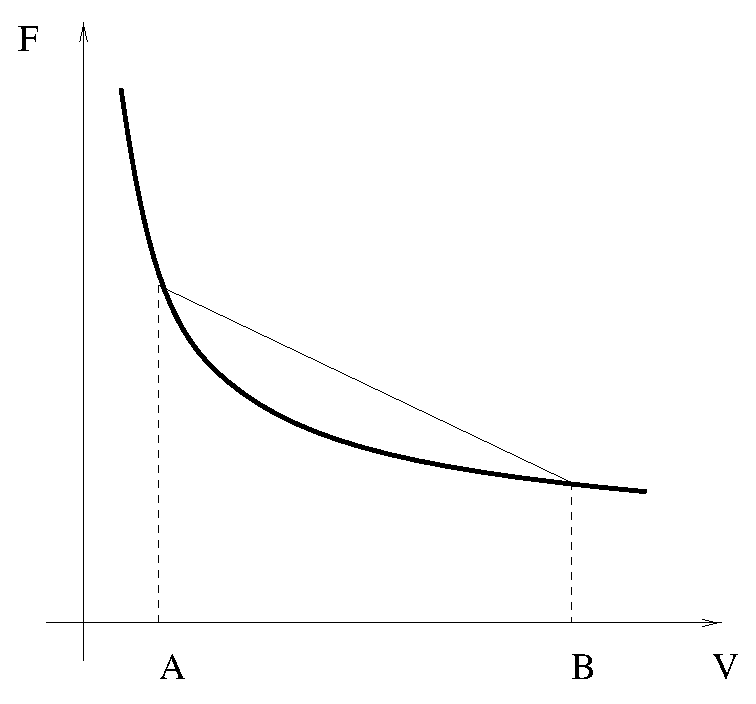
\epsfig{file={../fig/vanavant},width=6 cm,angle=-90}}   
 \caption{Au dessus de la temp\'erature critique, l'\'energie ne
pr\'esente pas 
de minimum local.}
 \label{figvanavant}
\end{figure}
\begin{figure}[htb]
 \centerline{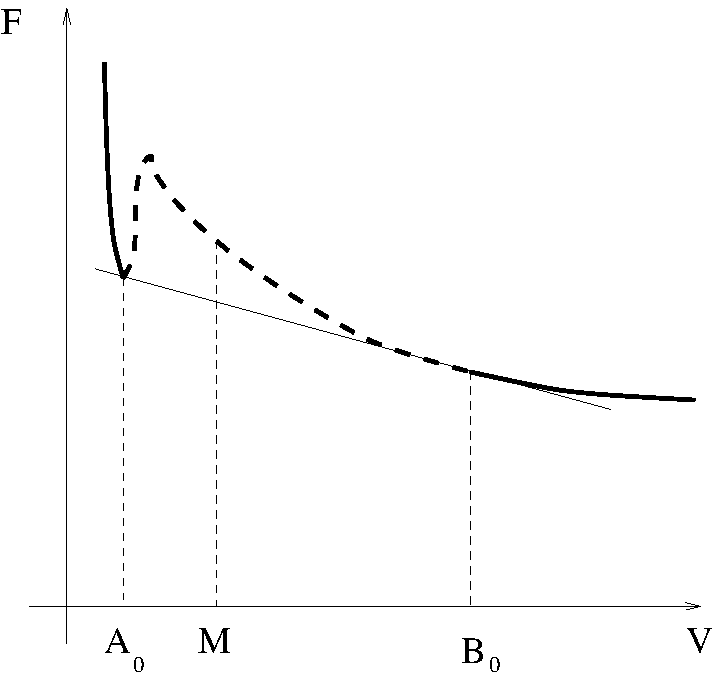
\epsfig{file={../fig/vanapres},width=6 cm,angle=-90}}   
 \caption{Au dessous de la temp\'erature critique, l'\'energie
pr\'esente un minimum local. Deux phases apparaissent alors,
caract\'eris\'ees par les points $A_{0}$ et $B_0$.}
 \label{figvanapres}
\end{figure}
Lorsque la temp\'erature est inf\'erieure \`a la temp\'erature
critique $T_c$, l'\'energie du syst\`eme pour un volume donn\'e $V_M$
avec $V_{A_0}<V_M<V_{B_0}$ n'est pas $F_v(V_M)$. En effet, le syst\`eme
\'evolue vers un \'etat d'\'energie inf\'erieure (voir figure
\ref{figvanapres}:  
\begin{equation}
F(V_M)=F_{A_0}+\frac{V_M-V_{A_0}}{V_{B_0}-V_{A_0}}(F_{B_0}-F_{A_0})
\end{equation}
L'apparition du minimum local de $F$ correspond \`a l'apparition de
deux phases.\index{transition de phase}
\section{Mod\`ele d'Ising}\label{secmodising}
%%%%%%%%%
Dans cette section, nous pr\'esentons un exemple de calcul de fonction
de partition. Cet exemple concerne le mod\`ele d'Ising\
\cite{ma:equad:Schuster88,ph:physt:LeBellac88,ph:physt:Diu89}. Le
mod\`ele d'Ising\index{Ising} est un 
mod\`ele du ferromagn\'etisme\index{ferromagn\'etisme}. Un corps
ferromagn\'etique est un 
corps constitu\'e de domaines de taille microscopiques poss\'edant un
petit moment magn\'etique. L'orientation de ces moments \'etant
al\'eatoire, le moment magn\'etique total du mat\'eriau est nul.
Cependant au--dessous d'une certaine temp\'erature critique $T_c$, les
moments magn\'etiques s'orientent suivant un certaine direction, et on
observe un moment magn\'etique total non nul\footnote{%%%%%%%
On dit qu'il y a transition de phase.\index{transition de phase}
Historiquement, on distingue 
deux types de transitions de phases \cite{ph:physt:Diu89}
\begin {enumerate}
\item la transition de phase du premier ordre
(par exemple la transition liquide-vapeur)
dont les caract\'eristiques sont :
\begin{enumerate}
\item Coexistence des deux phases.
\item La transition s'accompagne d'une variation d'entropie
\item existence d'\'etats m\'etastables.
\end{enumerate}
\item la transition de phase du deuxi\`eme  ordre
(par exemple la transition ferromagn\'etique--paramagn\'etique) dont
les caract\'eristiques sont : 
\begin{enumerate}
\item Brisure de sym\'etrie
\item L'entropie S est une fonction continue de la temp\'erature T et du
param\`etre d'ordre
\end{enumerate}
\end{enumerate}
}%%%%%%%%%%%%%%%
. Le mod\`ele d'Ising a
\'et\'e propos\'e pour d\'ecrire ce ph\'enom\`ene. Il consiste \`a
d\'ecrire chaque domaine de taille microscopique par un moment $S_i$
(que l'on peut consid\'erer comme un moment de spin)\index{spin} et \`a d\'ecrier
l'interaction entre les spins par l'hamiltonien suivant (syst\`eme \`a
une dimension) :
\begin{equation}
H=-K\sum S_lS_{l+1}
\end{equation}
La fonction de partition est
\begin{equation}
Z=\sum_{(S_l)}\Pi_{l=0}^{N-1}e^{-KS_lS_{l+1}},
\end{equation}
qui peut \^etre \'ecrite :
\begin{equation}
Z=\sum_{(S_l)}\Pi_{l=0}^{N-1}ch K +S_lS_{l+1}sh K
\end{equation}
On suppose que $S_l$ peut prendre deux valeurs possibles uniquement.
Bien que le mod\`ele d'Ising \`a une dimension ne pr\'esente pas de
transition de phase, nous allons illustrer le calcul de la fonction de
partition de deux mani\`eres.
$\sum_{(S_l)}$ repr\'esente une somme sur toutes les valeurs possibles
des $S_l$, c'est donc, de la m\^eme mani\`ere qu'une int\'egrale sur
un volume est l'int\'egrale successive sur chacune des variables, la
somme successive sur les $S_l$. On peut \'ecrire $Z$ comme :
\begin{equation}
Z=\sum_{S_1}\dots\sum_{S_n}f(S_1,S_2)f(S_2,S_3)\dots
\end{equation}
avec
\begin{equation}
f_{K}(S_i,S_{i+1})=ch K +S_iS_{i+1}sh K
\end{equation}
Nous avons
\begin{equation}
\sum_{S_1}f(S_1,S_2)=2 ch K
\end{equation}
En effet :
\begin{equation}
\sum_{S_1}f(S_1,S_2)=ch K +S_2 (+1)shK + ch K +S_2 (-1)shK 
\end{equation}
Donc en int\'egrant sur chaque variable successivement on obtient la
fonction de partition :
\begin{equation}\label{eqZisi}
Z=2^{n-1} (ch K)^{n-1}
\end{equation}

Nous
allons maintenant retrouver ce r\'esultat en utilisant une puissante
m\'ethode de calcul : la 
m\'ethode du {\bf groupe de
renormalisation}\cite{ph:physt:Diu89,ma:equad:Schuster88}\index{groupe de
renormalisation}\index{renormalisation (groupe de)}. 
Reprenons la fonction de partition sous sa forme :
\begin{equation}
Z=\sum_{S_1}\dots\sum_{S_n}f(S_1,S_2)f(S_2,S_3)\dots
\end{equation}
avec
\begin{equation}
f_{K}(S_i,S_{i+1})=ch K +S_iS_{i+1}sh K
\end{equation}
Regroupons par deux les termes :
\begin{equation}
Z=\sum_{S_1}\dots\sum_{S_n}g(S_1,S_2,S_3).g(S_3,S_4,S_5)\dots
\end{equation}
o\`u 
\begin{equation}
g(S_i,S_{i+1},S_{i+2})=(ch K +S_iS_{i+1}sh K)(ch K +S_{i+1}S_{i+2}sh K)
\end{equation}
Ce regroupement est illustr\'e par la figure \ref{figrenorm}
\begin{figure}[htb]
 \centerline{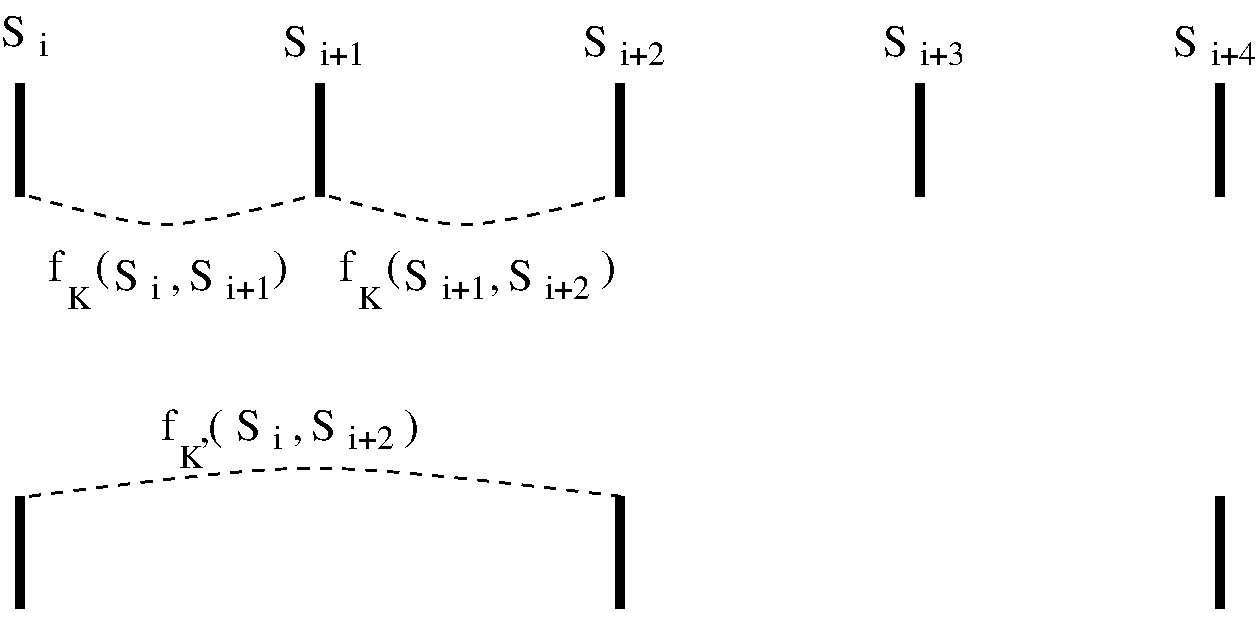
\epsfig{file={../fig/renorm},width=10 cm,angle=-90}}   
 \caption{La somme sur les valeurs possibles des spins
$S_{i},S_{i+1},S_{i+2}$ du produit
$f_K(S_i,S_{i+1})f_K(S_{i+1},S_{i+2})$ est la somme  sur les valeurs
possibles des spins 
$S_{i}$ et $S_{i+2}$ d'un fonction $f_{K'}(S_{i},S_{i+2})$ 
d\'eduite de $f_K$ par simple changement de la valeur du param\`etre
$K$ pr\'esent dans la d\'efinition de $f_K$.} 
 \label{figrenorm}
\end{figure}
Le calcul de la somme sur toutes les valeurs de $S_{i+1}$ possibles
donne :
\begin{equation}
\sum_{S_{i+1}}g(S_i,S_{i+1},S_{i+2})=2(ch^2K+S_{i}S_{i+2}sh^2K)
\end{equation}
La fonction $\sum_{S_{i+1}}g(S_i,S_{i+1},S_{i+2})$ peut donc \^etre mise 
sous la forme d'une autre fonction $f_{K'}(S_i,S_{i+2})$ avec
\begin{equation}
K'=Arcth(th^2K)
\end{equation}
En it\'erant le processus, on obtient une suite qui converge vers la
fonction de partition $Z$ donn\'ee par l'\'equation \ref{eqZisi}.
\begin{exo}
\'Etudier le mod\`ele d'Ising \`a deux dimensions. Peut--on encore envisager
une m\'ethode directe pour calculer $Z$ ? Ecrire un programme permettant de
visualiser l'\'evolution des spins au cours du temps en fonction de la
temp\'erature. 
\end{exo}
\section{Verre de spin}\label{secverredespi}
%%%%%%%%%%%%%%%%%%%%%%%%
Nous supposons que le syst\`eme de verre de spin\index{verre de spin}
poss\`ede une 
\'energie :
\begin{equation}
H=\sum J_{ij}S_iS_j
\end{equation}
Les valeurs des variables de spin $S_i$ sont plus ou moins un suivant
que le spin est orient\'e vers le bas ou vers le haut.
Le coefficient $J_{ij}$ vaut plus ou moins un suivant que les spins
$i$ et $j$ tendent \`a s'orienter dans le m\^eme sens ou dans des sens
oppos\'es. 
Dans un verre de spin la valeur de $J_{ij}$ est distribu\'ee au hasard
(suivant la position al\'eatoire des atomes portant le spin).
On note donc l'\'energie :
\begin{equation}
H_J=\sum J_{ij}S_iS_j
\end{equation}
o\`u $J$ donne la distribution des $J_{ij}$. La fonction de partition
est :
\begin{equation}
Z_J=\sum_{[s]}e^{-\beta H_J[s]}
\end{equation}
o\`u $[s]$ est une configuration  de spin. Nous cherchons \`a calculer
l'\'energie moyenne $\bar f$ sur les distributions de $J_{ij}$ :
\begin{equation}
\bar f=\sum_JP[J]f_J
\end{equation}
o\`u $P[j]$ est la fonction densit\'e de probabilit\'e des
configurations $[J]$ et o\`u $f_J$ est :
\begin{equation}
f_J=-\ln Z_J
\end{equation}
Cette mani\`ere de faire la moyenne n'est pas habituelle en physique
statistique. On fait la moyenne sur la variable $J$ ``tremp\'ees'',
c'est \`a dire variant tr\`es lentement par rapport aux $S_i$. Une
moyenne plus classique correspondrait \`a $\sum_J
P[J]\sum_{[s]}e^{-\beta H_J[s]}$ (les $J$ sont alors des variables
``recuites'').
Consid\'erons un syst\`eme $S_j^n$ compos\'e de $n$
r\'epliques\index{r\'epliques} du
m\^eme syst\`eme $S_J$. Sa fonction de partition $Z_J^n$ est simplement :
\begin{equation}
Z_J^n=(Z_J)^n
\end{equation}
Soit $f_n$ la moyenne sur $J$ d\'efinie par
\begin{equation}
f_n=-\frac{1}{n}\ln \sum_J P[J](Z_J)^n
\end{equation}
Comme :
\begin{equation}
\ln Z=\lim_{n\rightarrow 0}\frac{Z^n-1}{n}
\end{equation}
on a:
\begin{equation}
\lim_{n\rightarrow 0}f_n=\lim_{n\rightarrow 0}\ln (\sum_J P[J][1+n \ln Z_J])
\end{equation}
en posant utilisant $\sum_JP[J]=1$ et $\ln(1+x)=x+O(x)$ on a 
\begin{equation}
\bar f=\lim_{n\rightarrow 0}f_n
\end{equation}
On a donc remplac\'e une moyenne sur $\ln Z$ par une moyenne sur $Z^n$
au prix d'un prolongement analytique en z\'ero. Les cacluls se trouvent
alors grandement simplifi\'es\cite{ph:sping:Mezard87}.

Le calcul de l'\'etat d'\'equilibre d'un syst\`eme frustr\'e peut se
faire par la m\'ethode du {\bf recuit simul\'e}.\index{recuit simul\'e} Une impl\'ementation
num\'erique peut \^etre faite en utilisant l'algorithme de
M\'etropolis\index{M\'etropolis}. Cette m\'ethode peut \^etre
appliqu\'ee au probl\`eme du 
voyageur de commerce\cite{ma:compu:Press92}\index{probl\`eme du 
voyageur de commerce}.
\section{Gaz parfait quantiques}\label{secgazparfq}
%%%%%%%%%%%%%%%%%%%%%%%%%%%%%%%
\subsection{Introduction}
%%%%%%%%%%%%%%%%%%%%%%%%%
Consid\'erons un syst\`eme\index{gaz parfait quantique} en \'equilibre avec un r\'eservoir de
particules\cite{ph:physt:Diu89} et avec un thermostat. On dit que l'on
adopte une description grand-canonique. On montre que la solution du
probl\`eme de maximalisation de l'entropie (par la m\'ethode des
multiplicateurs de Lagrange) donne une probabilit\'e d'occupation d'un
\'etat $l$  d'\'energie $E_l$ et de nombre de particules $N_l$ est :
\begin{equation}
P_l=\frac{1}{Z}e^{-\beta E_l+\mu\beta N_l}
\end{equation}
avec
\begin{equation}
Z=\sum_le^{-\beta E_l+\mu\beta N_l}
\end{equation}
Consid\'erons un syst\`eme de particules ind\'ependantes identiques
indiscernables. L'\'etat $l$ peut alors \^etre d\'efini par la donn\'ee
des \'etats $\lambda$ des particules individuelles. 
\begin{figure}[htb]
 \centerline{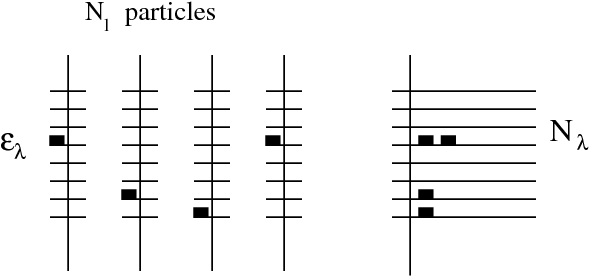
\epsfig{file={../fig/occup},width=6 cm,angle=-90}}   
 \caption{Un syst\`eme dont le nombre $N_l$ de particules
ind\'ependantes varie peut \^etre d\'ecrit par la donn\'ee de $N_l$
\'energies des particules, ou de mani\`ere \'quivalente par les
nombres $N_\lambda$ des diff\'erents niveaux d'\'energie
$\epsilon_\lambda$. }
 \label{figoccup}
\end{figure}
Soit
$\epsilon_\lambda$ l'\'energie d'une particule dans l'\'etat
$\lambda$.
L'\'energie du syst\`eme dans l'\'etat $l$ est alors :
\begin{equation}
E_l=\sum_\lambda N_\lambda \epsilon_\lambda
\end{equation}
o\`u $N_\lambda$ est le nombre de particules dans un \'etat
d'\'energie $E_\lambda$ (on l'appelle nombre d'occupation\index{nombre d'occupation} de l'\'etat
d'\'energie $E_\lambda$, voir la figure \ref{figoccup}). On a aussi :
\begin{equation}
N_l=\sum_\lambda N_\lambda
\end{equation}
La fonction de partition devient donc :
\begin{equation}
Z=\Pi_\lambda \xi_\lambda
\end{equation}
avec 
\begin{equation}
\xi_\lambda=\sum_{N_l}e^{-\beta N_\lambda\epsilon_\lambda+\beta
N_\lambda\mu} 
\end{equation}
Le nombre moyen de particules est d\'efini par :
\begin{equation}
\beta \bar N=-\frac{\partial \ln Z}{\partial \mu}
\end{equation}
qui peut s'\'ecrire :
\begin{equation}
\beta \bar N=\sum_\lambda N_\lambda
\end{equation}
o\`u $N_\lambda$ repr\'esente le  nombre moyen d'occupation et est
d\'efini par l'\'egalit\'e : 
\begin{equation}
\beta \bar N_\lambda=\frac{\partial \ln \xi_\lambda}{\partial \mu}
\end{equation}

\subsection{Gaz de fermions}
%%%%%%%%%%%%%%%%%%%%%%%%%%%
Si les particules sont des fermions,\index{fermions} d'apr\`es le
principe de Pauli\index{principe de Pauli},
le nombre d'occupation $N_\lambda$ ne peut prendre pour valeur que
z\'ero (aucune particule du syst\`eme ne poss\`ede une \'energie
$\epsilon_\lambda$) ou un (une seule particule du syst\`eme 
poss\`ede une \'energie $\epsilon_\lambda$).
L'expression de la fonction de partition permet alors de calculer les
propri\'et\'es thermodynamiques du syst\`eme, par exemple on peut
d\'eterminer les propri\'etes \'electroniques des {\bf m\'etaux et
semiconducteurs}\cite{ph:physt:Diu89}\index{m\'etal}\index{semi-conducteur}. Le gaz de fermions peut aussi
servir \`a d\'ecrire les {\bf naines blanches}\index{naine blanche}.
Les naines 
blanches\cite{ph:physt:Diu89} sont des 
\'etoiles tr\`es denses : leur masse est celle d'une \'etoile\index{\'etoile} ordinaire
(telle que le soleil) mais leur rayon est 50 \`a 100 fois plus petit.
La pression gravitationelle implique une contraction de l'\'etoile.
Cette pression est dans une \'etoile ordinaire compens\'ee par le
r\'eaction thermonucl\'eaire qui ont lieu dans le coeur de l'\'etoile.
Mais dans une naine blanche ces r\'eactions nucl\'eaires n'ont plus
lieu. Cependant, on peut montrer que la temp\'erature du gaz
d\'electron est tr\`es 
faible. Comme les \'electrons ne peuvent pas tous \^etre \`a
vitesse nulle d'apr\`es le principe de Pauli\footnote{En effet
l'\'etat d'un \'electron dans une 
bo\^\i te est 
uniquement d\'etermin\'e par son \'energie, la position de
l'\'electron n'\'etant d\'efinie en m\'ecanique quantique}, ils exercent
donc une pression. C'est cette pression, dite  ``quantique'', qui
compense la pression gravitationelle et emp\^eche l'\'etoile de
s'effondrer compl\`etement.

\subsection{Gaz de bosons}
%%%%%%%%%%%%%%%%%%%%%%%%%%%
Si les particules sont des fermions, d'apr\`es le principe de Pauli,
le nombre d'occupation $N_\lambda$ peut prendre toutes les valeurs
enti\`eres positives ou nulles :
\begin{equation}
\xi^B_\lambda= \sum_{N_\lambda=0}^{+\infty}e^{-\beta
N_\lambda\epsilon_\lambda+\beta N_\lambda\mu} 
\end{equation}
$\xi^B_\lambda$ repr\'esente la somme d'une s\'erie g\'eom\'etrique de
raison :
\begin{equation}
e^{-\beta \epsilon_\lambda+\beta \mu}
\end{equation}
o\`u $\epsilon_\lambda$ est fix\'e.
La s\'erie converge si 
\begin{equation}
\epsilon_\lambda-\mu>0
\end{equation}
On peut alors montrer\cite{ph:physt:Diu89} que, \`a basse temp\'erature,
les bosons s'accumulent dans l'\'etat de plus basse \'energie. Ce
ph\'enom\`ene est appel\'e condensation de Bose.\index{condensation de
Bose} 
\begin{rem}
Les photons sont des bosons dont le nombre n'est pas conserv\'e, ce
qui leur conf\`ere un comportement tr\`es particulier : leur potentiel
chimique est nul.
\end{rem}


\section{Probl\`emes \`a N corps et description cin\'etique}\label{desccinet}
%%%%%%%%%%%%%%%%
\subsection{Introduction}
%%%%%%%%%%%%%%%%%%%%%%
Dans cette section, nous revenons sur la description classique des
syt\`emes de particules d\'ej\`a abord\'ee \`a la section
\ref{secdistclassi}. On s'int\'eresse d\'esormais \`a la probabilit\'e
de pr\'esence d'une particule dans un volume \'el\'ementaire de
l'espace des phases. Nous proposons d'abord un mod\`ele simple qui
permet de retrouver la loi des gaz parfaits. Puis, nous faisons une excursion
hors du domaine de la thermodynamique de l'\'equilibre pour introduire
les \'equations d'\'evolutions dans le cadre d'une th\'eorie
cin\'etique. Ces \'equations peuvent \^etre utilis\'ee pour la
d\'emonstration des grandes lois de conservation de la m\'ecanique des
milieux continus (conservation de  la masse, de la quantit\'e de
mouvement, de l'\'energie,\dots) comme nous le verrons au chapitre
suivant. 
\subsection{Th\'eorie cin\'etique des gaz}
%%%%%%%%%%%%%%
On peut traiter le probl\`eme du gaz parfait\index{gaz parfait} dans
le cadre d'une 
th\'eorie cin\'etique\index{cin\'etique (description)}. Il s'agit d'un
point de vue plus proche  
de la m\'ecanique qui poss\`ede  l'avantage de mieux faire comprendre
la physique des ph\'enom\`enes.
Consid\'erons l'\'energie interne :
\begin{equation}
U=\sum \frac{1}{2}mv_i^2+V(r_1,\dots,r_N)
\end{equation}
Un \'etat du syst\`eme est d\'efini par les $r_i,p_i$. La
probabilit\'e pour que le syst\`eme soit dans cet \'etat est :
\begin{equation}
dP=\frac{1}{a}e^{-\beta[\sum \frac{1}{2}mv_i^2+V(r_1,\dots,r_N)]}
\end{equation}
La probabilit\'e pour qu'une particule ait la vitesse $v$ est :
\begin{equation}
dP(v)=\frac{1}{B}e^{-\beta \frac{1}{2}mv^2}dv_xdv_ydv_z
\end{equation}
$B$ est \`a d\'eterminer par $\int P =1$.
\begin{equation}
dP(v_x)=N\sqrt{\frac{m}{2\pi k_BT}}e^{-\beta \frac{1}{2}mv_x^2}dv_x
\end{equation}
C'est une gaussienne. On sait :
\begin{equation}
\overline{v_x}=0
\end{equation}
\begin{equation}
\overline{v^2_x}=\frac{k_BT}{m}
\end{equation}
Donc :
\begin{equation}
\overline{\frac{1}{2}mv^2_x}=\frac{1}{2}k_BT
\end{equation}
Ce r\'esultat est en accord avec le th\'eor\`eme d'\'equipartition de
l'\'energie. Toute particule qui traverse $\Sigma$ fait augmenter  de
$mv_z$ la quantit\'e de mouvement.
Dans toute la bo\^\i te le nombre de mol\'ecules qui ont leur vitesse entre
$v_z$ et $v_z+dv_z$ est (voir fig.\ref{figboite})
\begin{figure}[htb]
 \centerline{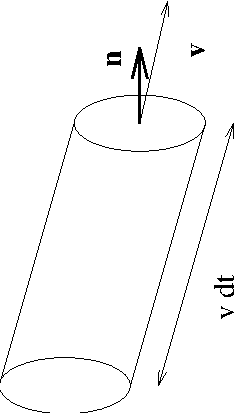
\epsfig{file={../fig/boite},width=6 cm,angle=-90}}   
 \caption{Quantit\'e de mouvement c\'ed\'ee par les particules dans un
volume \'el\'ementaire.}
 \label{figboite}
\end{figure}

\begin{equation}
dN=NP(v_z)dv_z
\end{equation}
Dans un volume $\Delta V$ :
\begin{equation}
\Delta(dN)=N\frac{\Delta V}{V}P(v_z)dv_z
\end{equation}
On choisit $\Delta V =s v_z \Delta t$.
L'accroissement de la quantit\'e de mouvement est \'egale \`a la
puissance de force de pression.
\begin{equation}
\int_{-\infty}^{+\infty}m v_z.N\frac{\Delta V}{V}P(v_z)dv_z=p s \Delta t
\end{equation}
D'o\`u
\begin{equation}
pV=Nk_BT
\end{equation}
C'est bien l'\'equation d'\'etat des gaz parfaits d\'emontr\'ee \`a la
section \ref{secgazparfthe}.
\subsection{Description cin\'etique}\label{secdesccinet}
%%%%%%%%%%%%%%%%
Introduisons 
\begin{equation}
w(r_1,p_1,\dots,r_n,p_n)dr_1\dots dr_n dp_1\dots dp_n,
\end{equation}
la probabilit\'e pour que la particule $1$ soit dans le volume de
l'espace des phases compris entre $r_1,p_1$ et $r_1 +dr_1,p_1+dp_1$, la particule $2$ dans le volume de
l'espace des phases compris entre $r_2,p_2$ et $r_2 +dr_2,p_2+dp_2$,\dots,
la particule $n$ dans le volume de
l'espace des phases compris entre $r_n,p_n$ et $r_n +dr_n,p_n+dp_n$.
Comme les particules sont indiscernables,
\begin{equation}
\frac{1}{N!}w(r_1,p_1,\dots,r_n,p_n)dr_1\dots dr_n dp_1\dots dp_n
\end{equation}
est la probabilit\'e\footnote{\`A l'\'equilibre thermodynamique, on a
vu que  $w(r_1,p_1,\dots,r_n,p_n)$ s'\'ecrit:
\begin{equation}
w(r_1,p_1,\dots,r_n,p_n)=ae^{-\beta[\sum
\frac{1}{2}mv_i^2+V(r_1,\dots,r_N)]} 
\end{equation}
}%%%%%endfoot
pour qu'une particule  soit dans le volume de
l'espace des phases compris entre $r_1,p_1$ et $r_1 +dr_1,p_1+dp_1$,
une autre particule dans le volume de
l'espace des phases compris entre $r_2,p_2$ et $r_2 +dr_2,p_2+dp_2$,\dots,
et une $n$--i\`eme particule dans le volume de
l'espace des phases compris entre $r_n,p_n$ et $r_n +dr_n,p_n+dp_n$.
Nous avons la condition de normalisation :
\begin{equation}
\int w dr_1\dots dr_n dp_1\dots dp_n=1
\end{equation}
D'o\`u par d\'erivation :
\begin{equation}
\int \frac{dw}{dt} dr_1\dots dr_n dp_1\dots dp_n+\int w\frac{d
(dr_1\dots dr_n dp_1\dots dp_n)}{dt}=0 
\end{equation}
Si le syst\`eme est hamiltonien\index{hamiltonien (syst\`eme)}, l'\'el\'ement de volume est conserv\'e,
donc on a l'{\bf \'equation de Liouville} :
\begin{equation}
\frac{dw}{dt}=0
\end{equation}
Cette \'equation devient en tenant compte de la d\'efinition de $r$ et
$p$ : 
\begin{equation}
\frac{\partial w}{\partial t}+\{w,H\}=0
\end{equation}
o\`u $H$ est l'hamiltonien du syst\`eme. On pose la fonction de
r\'epartition : 
\begin{equation}
f_1(r,p,t)=\frac{1}{(N-1)!}\int w \Pi_{i=2}^n dr_idp_i
\end{equation}
D'o\`u, en int\'egrant l'\'equation de Liouville :
\begin{equation}
\frac{\partial f_1}{\partial t}=\frac{1}{(N-1)!}\int \{H,w\} \Pi_{i=2}^n dr_idp_i
\end{equation}
et en supposant 
\begin{equation}
H=\sum p_i/2m+\sum u_{ij},
\end{equation}
on obtient une hi\'erarchie d'\'equations (appel\'ee 
{\bf hi\'erarchie BBGKY}\index{hi\'erarchie BBGKY}) liant les fonctions
$f_k(r_1,p_1,\dots,r_k,p_k,t)$ d\'efinies par :
\begin{equation}
f_k(r_1,p_1,\dots,r_k,p_k,t)=\frac{1}{(N-k)!}\int w \Pi_{i=k+1}^n
dr_idp_i
\end{equation} 
On peut prendre une condition de fermeture de la hi\'erarchie.
Vlasov prend la condition suivante :
\begin{equation}
f_2(r_1,p_1,r_2,p_2)=f_1(r_1,p_1)f_2(r_2,p_2)
\end{equation}
et on obtient l'{\bf \'equation de Vlasov}\index{Vlasov (\'equation de)} :
\begin{equation}
[\frac{\partial}{\partial t}+\frac{p}{m}\frac{\partial}{\partial r}+[F-\frac{\partial \bar{u}}{\partial r}]\frac{\partial }{\partial p}]f_1=0
\end{equation}
o\`u $\bar{u}$ est le potentiel moyen.
on peut donc r\'e\'ecrire l'\'equation de Vlasov en introduisant une force
efficace $F_e$ qui d\'ecrit ls forces subies par les particules dans une
approximation de champ moyen :
\begin{equation}\label{eqvlasov}
[\frac{\partial}{\partial t}+\frac{p}{m}\frac{\partial}{\partial r}+F_e\frac{\partial }{\partial p}]f_1=0
\end{equation}
Les diff\'erents moments de l'\'equation de Valsov permettent de
d\'emontrer les \'equation de conservation de la m\'ecanique des
milieux continus (voir chapitre \ref{chapapproxconti}).
\begin{rem}
Une variante de l'\'equation de Vlasov est l'{\bf \'equation de
Boltzman}\index{Boltzman}(voir \cite{ph:physt:Diu89}. les deux \'equations
diff\`erent sur la mani\`ere de traiter les collisions.
\end{rem}

\section{Exercices}
%%%%%%%%%%%%%%%%%%%
\begin{exo}
{\bf Paramagn\'etisme.} Consid\'erons un syst\`eme constitu\'e d'un nombre $N$
grand d'atomes situ\'es aux noeuds d'un r\'eseau cristallin. Soit $J_i$ le
moment cin\'etique total d'un atome $i$ dans son \'etat fondemental. On sait
qu'\`a un tel moment cin\'etique est associ\'e un moment magn\'etique :
\begin{equation}
\mu_i=-g\mu_BJ_i
\end{equation}
o\`u $\mu_B$ est le magn\'eton de Bohr et $g$ le facteur de Land\'e. $J_i$ ne
peut prendre que des valeurs demi--enti\`eres.

On suppose que le hamiltonien du syst\`eme des $N$ atomes est :
\begin{equation}
H=\sum -\mu_i B_0
\end{equation}
o\`u $B_0$ est un champ ext\'erieur.
\`A quel type de syst\`eme a--t--on affaire ? (syst\`eme de particules
discernables ou indiscernables ?) 
Trouver la fonction de partition du syst\`eme.
\end{exo}

\begin{exo}
On consid\`ere un gaz de Fermions ind\'ependants. Calculer le nombre
d'occupation moyen $\bar 
N_\lambda$ d'un \'eta $\lambda$ (On dit que $\bar N_\lambda$ suit la
distribution de Fermi).   
\end{exo}

\begin{exo}
On consid\`ere un gaz de Bosons ind\'ependants. Calculer le nombre
d'occupation moyen $\bar 
N_\lambda$ d'un \'eta $\lambda$ (On dit que $\bar N_\lambda$ suit la
distribution de Bose).   
\end{exo}

\begin{exo}
On consid\`ere un {\bf m\'etal conducteur.} On mod\'elise les \'electrons
libres du 
m\'etal par un gaz de Fermions ind\'ependants. On suppose que les \'etats du
syst\`eme peuvent \^etre d\'ecrits par une densit\'e d'\'etat $\rho(\epsilon)$,
$\epsilon$ \'etant l'\'energie d'un \'etat. Donner l'expression l'expression
de $\rho(epsilon)$. Trouver l'expression reliant le
nombre $\bar N$ d'\'electrons au potentiel chimique. Donner l'expression du
potentiel chimique dans le cas o\`u la temp\'erature est nulle. 
\end{exo}

\chapter{Approximation continue}\label{chapapproxconti}
%%%%%%%%%%%%%%%%%%%%%%%%%
\section{Introduction}
%%%%%%%%%%%%%%%%%%%%%%
Il existe plusieurs m\'ethodes pour introduire l'approximation
continue de la mati\`ere. Elles consistent en diff\'erentes approches du
probl\`eme de moyennisation sur les grandeurs des particules.
La premi\`ere approche consiste \`a partir de la m\'ecanique classique
et de consid\'erer les moyennes sur des volumes \'el\'ementaires
appel\'es \'el\'ements de fluide.
\begin{figure}[htb]
 \centerline{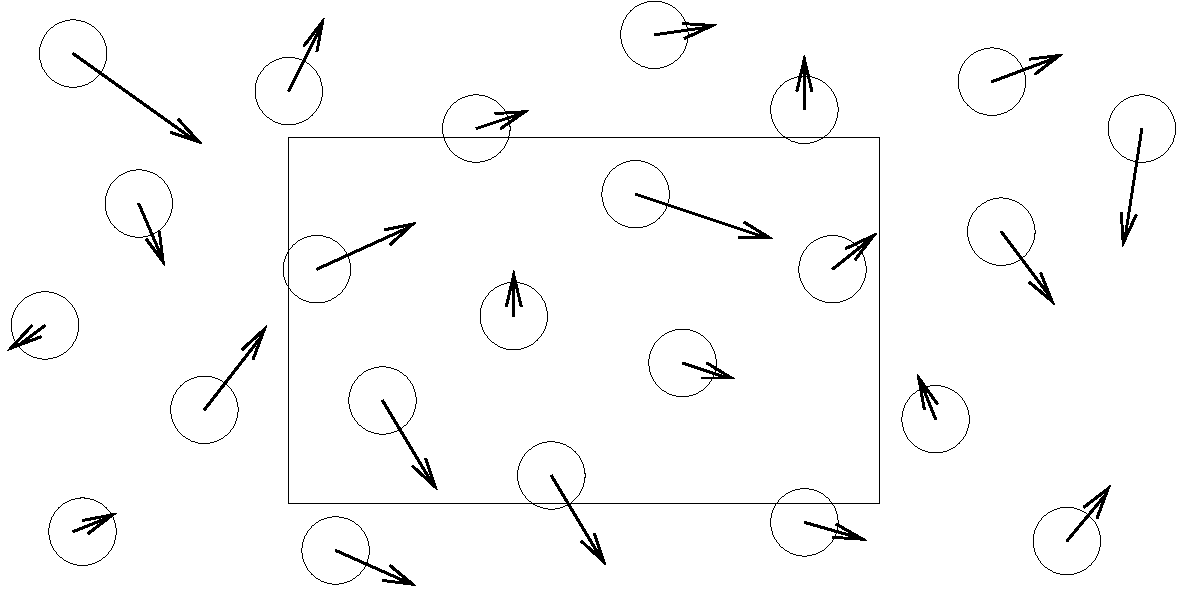
\epsfig{file={../fig/volele},width=6 cm,angle=-90}}   
 \caption{Les moyennes sont faite dans la boite \'el\'ementaire de
volume $d\tau$.}
 \label{figvolele}
\end{figure}
Consid\'erons un volume \'el\'ementaire $d\tau$ centr\'e en $r$, \`a
l'instant $t$. La figure \ref{figvolele} illustre cette m\'ethode de
moyennisation. Les grandeurs associ\'ees \`a l'approximation continue
s'obtiennent par divers passages \`a la limite lorsque le volume de la
bo\^\i te tend vers z\'ero. 
Ainsi la densit\'e en particules sera l'extrapolation de la limite
lorsque le volume de la bo\^\i te tend vers z\'ero du rapport du
nombre $dn$ de particules dans la bo\^\i te sur le volume $d\tau$ de la 
bo\^\i te :
\begin{equation}
n(r,t)=\lim_{d\tau\rightarrow 0}\frac{dn}{d\tau}
\end{equation}
De m\^eme, la vitesse moyenne du milieu sera :
\begin{equation}
v(r,t)=\lim_{d\tau\rightarrow 0}\frac{dv}{dn}
\end{equation}
o\`u $dv$ est la somme des vitesses des $dn$ particules pr\'esentes
dans la bo\^\i te.
\begin{rem}
Un tel passage \`a la limite est difficile \`a formaliser sur le plan
math\'ematique. Il s'agit d'une ``limite de physicien'' ! 
\end{rem}
\begin{rem}
Il faut noter que le rapport entre les grandeurs des particules et les
grandeur moyennes ne sont pas toujours \'evidents. Il peut arriver que
les vitesses des particules soient non nulles mais que  la vitesse du fluide
soit nulle. C'est le cas si les particules subissent une agitation
thermique. Mais il peut aussi arriver que  la moyenne temporelle des 
vitesses individuelles des particules  soit nulle mais que la vitesse
de l'\'el\'ement de fluide soit non nulle. La figure \ref{figvitnonul}
illustre cette remarque dans le cas du ph\'enom\`ene de
d\'erive\cite{ph:plasm:Chen84}. 
\begin{figure}[htb]
 \centerline{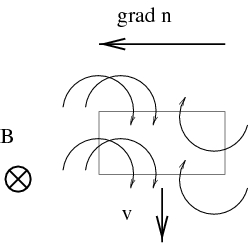
\epsfig{file={../fig/vitnonul},width=6 cm,angle=-90}}   
 \caption{Des \'electrons dans un champ magn\'etique $B$ poss\`edent un
mouvement circulaire uniforme. La moyenne temporelle du d\'eplacement de
chaque particule est donc nulle. N\'eanmoins, s'il existe un gradient de
concentration, la vitesse fluide est non nulle (ici dirig\'ee vers le
bas). C'est le ph\'enom\`ene de ``d\'erive'' courant dans les plasmas. }
 \label{figvitnonul}
\end{figure}
\end{rem}

Une autre m\'ethode consite \`a consid\'erer la fonction de
r\'epartion \`a une particule $f(r,p,t)$ introduite \`a la section
\ref{secdesccinet}. Rappelons que $\frac{1}{n}f(r,p,t)drdp$
repr\'esente la probabilit\'e de trouver \`a l'instant $t$ une
particule dans un volume de l'espace des phases compris entre $r,p$ et
$r+dr,p+dp$. 
Les diff\'erentes grandeurs fluides sont alors introduites comme les
diff\'erents moments de $f$ par rapport \`a la vitesse. Par exemple la
densit\'e de particule est le moment d'ordre z\'ero de $f$ :
\begin{equation}
n(r,t)=\int f(r,p,t)dp
\end{equation}
ce qui revient \`a dire que le nombre moyen de particule dans un
volume $d\tau$ est 
\begin{equation}
dn=n(r,t)d\tau.
\end{equation}
La vitesse fluide est li\'ee au premier moment de $f$ :
\begin{equation}
mv(r,t)=\int pf(p,r,t)dp
\end{equation}
L'objet de ce chapitre est de pr\'esenter les lois r\'egissant la
dynamique d'un syst\`eme continu. Ces lois se mettent sous la forme
g\'en\'erale d'une loi de conservation.
\section{Lois de conservation}
%%%%%%%%%
\subsection{Forme int\'egrale d'une loi de conservation}
%%%%%%%%%%%%%%%%
Une loi de conservation\index{conservation (loi de)} est un bilan qui
s'applique \`a tout domaine 
connexe, strictement int\'erieur au syst\`eme \'etudi\'e, et que l'on
suit dans son mouvement. Une telle  loi peut s'\'ecrire :
\begin{equation}
\frac{d}{dt}\int_D A_idv+\int_{\partial D} \alpha_{ij}
n_jd\sigma=\int_D a_idv \label{eqcon}
\end{equation}
Le symbole $\frac{d}{dt}$ d\'esigne la d\'eriv\'ee particulaire
(voir \ref{chapretour}).
$A_i$ est une fonction scalaire ou tensorielle des variables $x$ et $t$
euleriennes. $A$ est la densit\'e volumique de la quantit\'e ${\cal
A}$ (masse, quantit\'e de mouvement, \'energie, ...). $a_i$ est le 
taux de densit\'e volumique fourni par l'ext\'erieur. $\alpha_{ij}$ est
le taux de densit\'e surfacique de ce qui est perdu par le syst\`eme
\`a travers la fronti\`ere de $D$.
\subsection{Forme locale d'une loi de conservation}
%%%%%%%%%%%%%%%%
L'\'equation \ref{eqcon} repr\'esente la forme int\'egrale d'une loi de
conservation. \`A cette forme int\'egrale est associ\'ee une forme
locale que nous pr\'esentons maintenant.
D'apr\`es l'annexe \ref{chapretour}, nous avons l'\'egalit\'e : 
\begin{equation}
\frac{d}{dt}\int_D A_idv=\int_D \frac{d}{dt} A_idv
\end{equation}
On sait aussi :
\begin{equation}
\frac{dA_i}{dt}=\frac{\partial A_i}{\partial t}+(A_iu_j)_{,j}
\end{equation}
La formule de Green permet de passer d'une int\'egrale de surface \`a
une int\'egrale de volume : :
\begin{equation}
\int_{\partial D} \alpha_{ij}n_jd\sigma=\int_{D} \alpha_{ij,j}dv
\end{equation}
L'\'equation finale est donc :
\begin{equation}
\frac{\partial A_i}{\partial t}+(A_iu_j+\alpha_{ij})_{,j}=a_i
\end{equation}
Introduisons maintenant les diff\'erentes lois de conservation. 
\section{Conservation de la mati\`ere}
%%%%%%%%%%%%%%%%%%%%%%%%%%%%%%%%%%%%%
En prenant $A_i=\rho=\frac{dm}{d\tau}$, la masse volumique dans
l'\'equation \ref{eqcon} 
la densit\'e volumique, on obtient :
\begin{equation}
\frac{\partial \rho}{\partial t}+\dive (\rho u)=0
\end{equation}
Cette loi peut \^etre d\'emontr\'ee par des calculs sur des volumes
fluides \'el\'ementaires. Ainsi la variation de la masse $M$ dans un
volume $d\tau$ par unit\'e de temps est l'oppos\'e du flux de masse
sortant :
\begin{equation}
\frac{dM}{dt}=-\int_{d\tau} \rho v dr
\end{equation}
La forme locale de cette \'equation de conservation est donc :
\begin{equation}
\frac{\partial \rho}{\partial t}+\dive (\rho u)=0
\end{equation}

Mais cette loi peut \^etre aussi d\'emontr\'ee en prenant le premier
moment de l'\'equation  de Vlasov (\'equation {eqvlasov}). D\'efinissons la masse volumique
comme le moment d'ordre z\'ero de la fonction de r\'epartition
multipli\'ee par la masse : 
\begin{equation}
\rho=m\int dpf(r,p,t)
\end{equation}
Alors, en prenant le premier
moment de l'\'equation  de Vlasov on obtient \`a nouveau :
\begin{equation}
\frac{\partial \rho}{\partial t}+\nabla (\rho v)=0
\end{equation}

Une \'equation parfaitement analogue est celle de la conservation de
la charge.
L'\'equation locale traduisant la conservation de la charge a
exactement la m\^eme forme que l'\'equation de conservation de la
mati\`ere :
\begin{equation}
\frac{\partial \rho}{\partial t}+\dive{j}=0
\end{equation}
o\`u $j$ est la densit\'e de courant :
\begin{equation}
j=\rho v
\end{equation}
Le flux de $j$ \`a travers une surface ouverte $S$ est habituellement
appel\'e courant \'electrique tranversant $S$.

\section{Conservation de la quantit\'e de mouvement}
%%%%%%%%%%%%%%
Nous supposons que les forces ext\'erieures sont mod\'elis\'ees par
$f$. Les efforts int\'erieurs sont mod\'elis\'es par un tenseur
$\tau_{ij}$.
\begin{equation}
\frac{d}{dt}\int_D \rho u_idv+\int_{\partial D} \tau_{ij}
n_jd\sigma=\int_D f_idv 
\end{equation}
Cette \'equation int\'egrale correspond \`a l'application de la
relation fondamentale de la dynamique\index{impulsion} sur un volume
de fluide 
\'el\'ementaire comme l'indique la figure \ref{figconsp}.
\begin{figure}[htb]
 \centerline{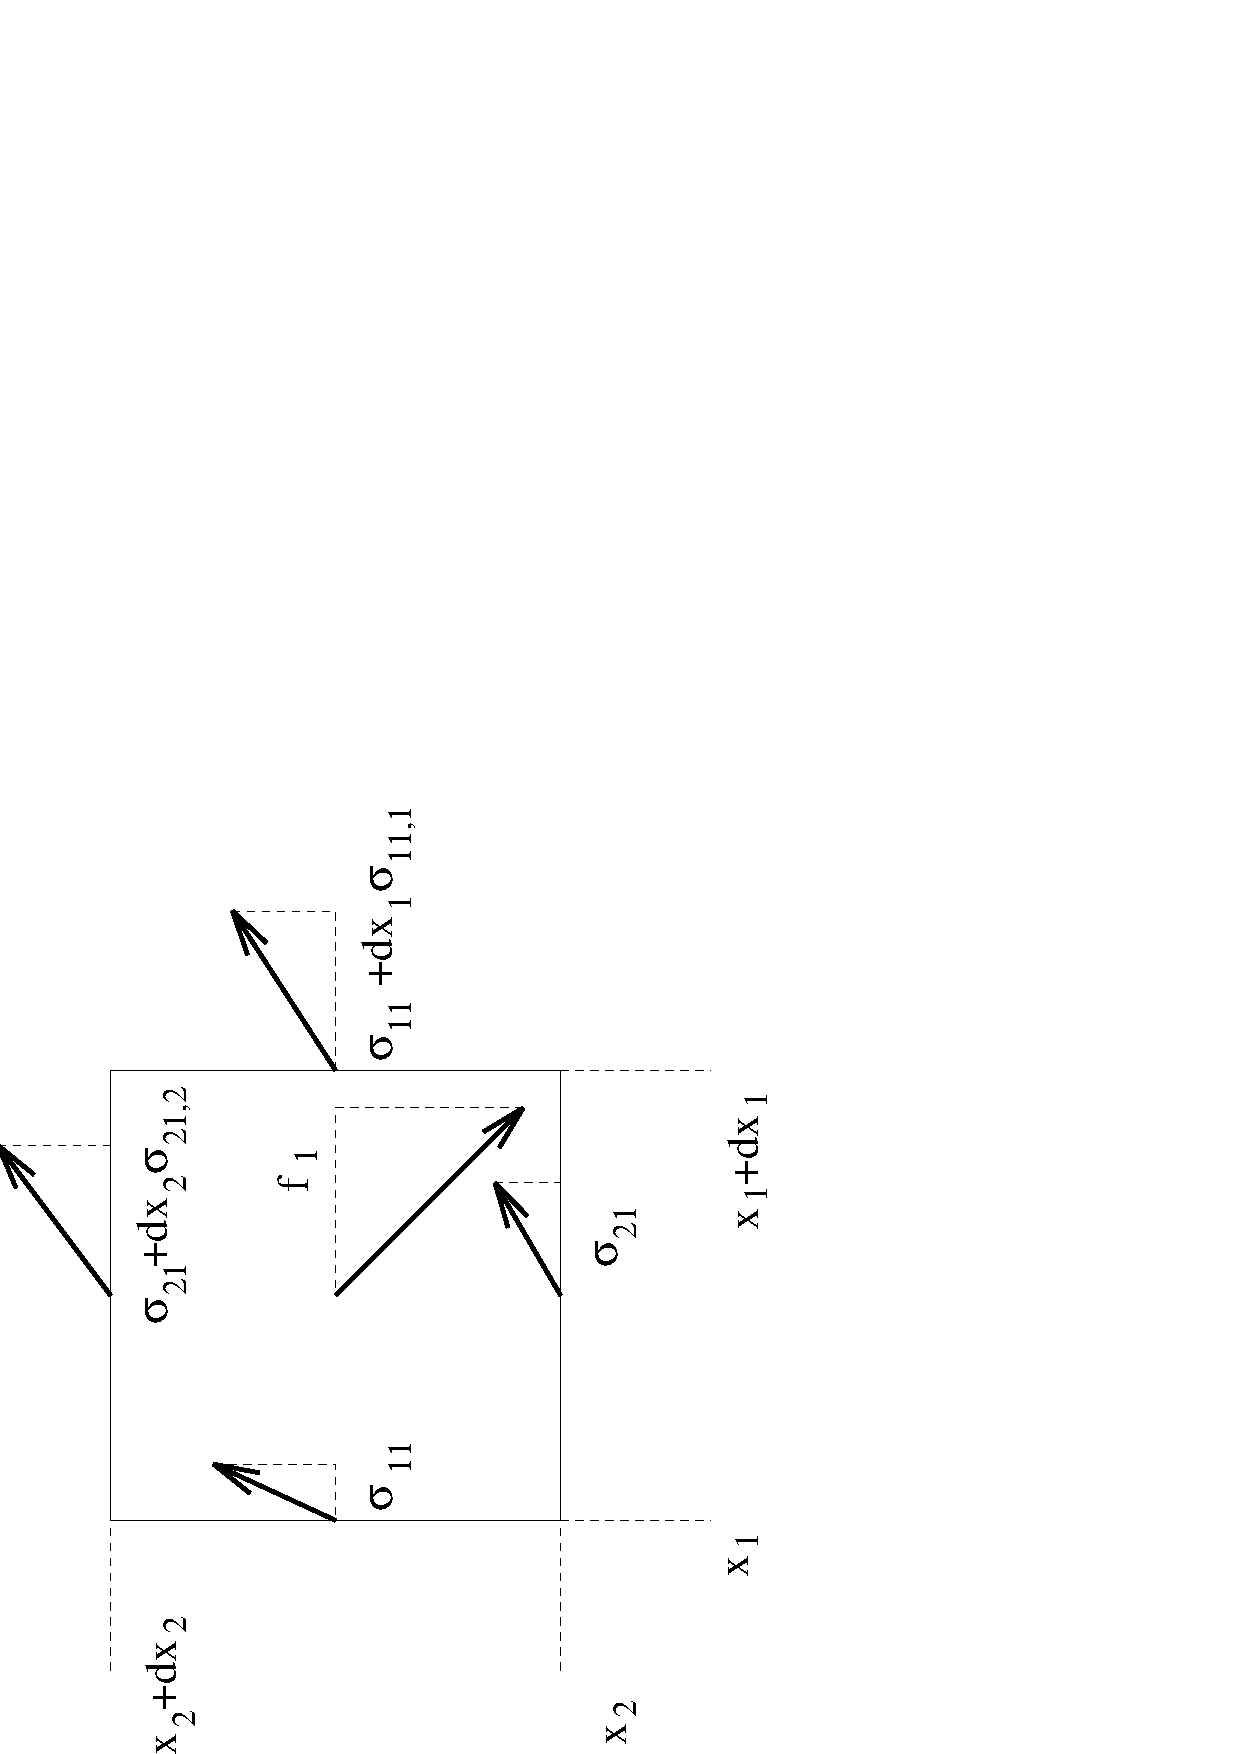
\epsfig{file={../fig/consp},width=6 cm,angle=-90}}   
 \caption{La conservation de la quantit\'e de mouvement correspond \`a
l'application de la relation fondamentale de la dynamique sur un
volume de fluide \'el\'ementaire.}
 \label{figconsp}
\end{figure}
L'\'equation aux d\'eriv\'ees partielles associ\'ee est :
\begin{equation}
\frac{\partial}{\partial t}(\rho u_i)+(\rho u_i u_j)_{,j}+\tau_{ij,j}=f_i
\end{equation}
En utilisant l'\'equation de continuit\'e, on obtient :
\begin{equation}
\rho(\frac{\partial}{\partial t}u_i+u_j u_{i,j})+\tau_{ij,j}=f_i
\end{equation}

\begin{rem}
On peut d\'emontrer la conservation de l'impulsion en prenant le
premier moment de l'\'equation  de Vlasov. L'impulsion du fluide $\bar p$ est
alors 
reli\'ee \`a la fonction de r\'epartition par l'\'egalit\'e suivante :
\begin{equation}
\bar p=\int p dp f(r,p,t)
\end{equation}
\end{rem}
Par la suite on d\'esigne l'impulsion du fluide simplement par $p$.
\section{Principe des puissances virtuelles}\label{secpuisvirtu}
%%%%%%%%%%%%%%%%%
\subsection{\'Enonc\'e du principe}
%%%%%%%%%
Nous avons introduit la conservation de la quantit\'e de mouvement par
des moyennes sur les particules des grandeurs associ\'ees aux
particules. Il nous a fallu mod\'eliser les forces \`a distances par
une densit\'e de force $f_i$, les efforts int\'erieurs par un
tenseur du second ordre $\tau_{ij}$,\dots
Nous abordons ici un point de vue dual o\`u les efforts sont
mod\'elis\'es par des fonctionelles.

En guise d'introduction au principe des puissances
virtuelles\index{virtuelles (puissances)}, citons
Germain reproduit dans \cite{ma:equad:Dautray1} :
``En M\'ecanique, il y a deux mani\`eres de sch\'ematiser, par
des concepts math\'ematiques des efforts s'exer\c cant \`a un instant
$t$ sur un syst\`eme mat\'eriel.
La premi\`ere consiste \`a repr\'esenter une force par un vecteur. On
g\'en\'eralise ici en repr\'esentant sur un syst\`eme par un champ
associ\'e \`a une mesure : champ de forces volumiques, surfaciques,
lin\'e\"\i ques\dots Lorsque les efforts sont ainsi sch\'ematis\'es,
il est clair que le principe fondamental de la dynamique est tout
indiqu\'e comme base de r\'esolution des probl\`emes.

La seconde voie est celle des puissances (ou travaux) virtuelles et est
bas\'ee sur des observations du type suivant :
\begin{itemize}
\item Lorsqu'on veut voir si une valise est lourde, on la soul\`eve.
\item Pour appr\'ecier la tension d'une couroie, on essaye de
l'\'ecarter de sa position d'\'equilibre.
\item C'est en essayant de pousser une voiture que l'on se rend compte
des frottements tant ext\'erieurs (route sur pneus) qu'int\'erieurs
(le frein \`a main est-il mis?).
\end{itemize}
On d\'etecte, dans ce second point de vue, les forces ext\'erieures et
int\'erieures \`a un syst\`eme, non directement, mais par l'effet
qu'elles produisent lorsque ce syst\`eme subit un d\'eplacement, une
vitesse, une d\'eformation; on les d\'etermine par la puissance
qu'elles d\'eveloppent dans un mouvement quelconque. L'id\'ee
math\'ematique essentielle sous-jacente est ici celle de la dualit\'e.
Cette deuxi\`eme voie, inspir\'ee ainsi par l'exp\'erience la plus
commune, pr\'esente l'int\'er\^et d'\'evaluer des efforts, en
g\'en\'eral mal d\'efinis par le premier point de vue, comme ceux de
liaison; elle est tr\`es souple aussi, car, selon que l'on choisira un
ensemble de mouvement virtuel plus ou moins vaste, on aura une
description des efforts plus ou moins fine''.
 \'Enoncons le principe des puissances virtuelles :
\begin{prin}
La puissance virtuelle des quantit\'es d'acc\'el\'eration est \'egale
\`a la somme 
des puissances virtuelles de tous les efforts appliqu\'es au syst\`eme
tant 
ext\'erieurs qu'int\'erieurs. Soit :
\begin{equation}
\int \rho \gamma_i \hat{u}_i
d\tau=P^{int}+P^{ext}_{dist}+P^{ext}_{contact} 
\end{equation}
o\`u $P^{int}$ repr\'esente les efforts int\'erieurs,
$P^{ext}_{dist}$,les efforts ext\'erieurs \`a distance,
$P^{ext}_{contact}$ les efforts ext\'erieurs de contact.
\end{prin}
\`A la section
\ref{sepripuiva} nous montrons comment un
syst\`eme d'\'equations aux d\'eriv\'ees partielles peut \^etre
consid\'er\'e comme un probl\`eme variationnel.
Ici, nous pr\'esentons une approche purement variationelle de la
m\'ecanique gr\^ace au principe des puissances virtuelles (voir aussi
la section \ref{sepripuiva}). Cette approche nous donne un moyen
puissant de mod\'eliser les efforts int\'erieurs et ext\'erieurs au
syst\`eme comme nous allons le voir dans la section \ref{seccasflu}
qui suit. En effet, on mod\'elise ici les efforts par des
fonctionnelles c'est-\`a-dire des applications
\begin{equation}
\begin{array}{llll}
P:&L(A,E)&\longrightarrow &R\\
  &u(r)&\longrightarrow &P(u(r))
\end{array}
\end{equation}
o\`u $A$ est l'espace affine attach\'e \`a $E$.

\subsection{Puissances virtuelles et \'equation locale}\label{sepripuiva}
%%%%%%%%%%
Nous pr\'esentons ici sur un cas particulier le lien entre la formulation
locale (\'equation aux d\'eriv\'ees partielles ou "EDP") et le principe des
puissances virtuelles (formulation variationnelle de 
l'EDP consid\'er\'ee).
Consid\'erons le probl\`eme :
\begin{prob}
Trouver $u$ tel que :
\begin{equation}
\partial_j\sigma_{i,j}(u)+f_i=0\ {\rm dans}\ \Omega
\end{equation}
\begin{equation}
u_i=0\ {\rm sur}\ {\rm sur}\ \Gamma_1
\end{equation}
\begin{equation}
\sigma_{i,j}(u)n_j=0\ {\rm sur}\ {\rm sur}\ \Gamma_2
\end{equation}
avec $\Gamma_1\cup\Gamma_2=\partial\Omega$.
\end{prob}
Introduisons la forme bilin\'eaire :
\begin{equation}
a(u,v)=\int_\Omega \sigma_{i,j}(u)\epsilon_{i,j}(v)dx
\end{equation}
On peut montrer que cette forme est $V$--elliptique.
D'autre part, la forme 
\begin{equation}
L(v)=\int_\Omega
f_iv_idx+\int_{\Gamma_1}g_iv_idx
\end{equation}
 est lin\'eaire continue sur $V$.
Donc il existe une fonction $u\in V$ unique telle que 
\begin{equation}
\forall v\in V, a(u,v)=L(v)
\end{equation}
$a(u,v)$ est  le travail de d\'eformation du solide\index{virtuelle
(puissance)} 
\'elastique\index{\'elastictit\'e} correspondant au d\'eplacement
virtuel $v$ \`a partir de 
la position $u$.
$L(v)$ est le travail des forces ext\'erieures pour le d\'eplacement
virtuel $v$.
Le principe des puissances virtuelles peut donc \^etre envisag\'e comme une
cons\'equence des grandes lois de conservation :
\begin{prin}{\bf Principe des puissances virtuelles (Cas statique):}
Le d\'eplacement r\'eel $u$ est le d\'eplacement cin\'ematiquement
admissible pour lequel le travail de d\'eformation du solide
\'elastique correspondant au d\'eplacement virtuel $v$ est \'egal au
travail des forces ext\'erieures, ceci pour tout d\'eplacement virtuel
$v$ cin\'ematiquement admissible.
\end{prin}
De plus comme $a(.,.)$ est sym\'etrique $u$ est le minimum de :
\begin{equation}
J(v)=\frac{1}{2}\int_\Omega
\sigma_{i,j}(v)\epsilon_{i,j}(v)dx-(\int_\Omega 
f_iv_idx+\int_{\Gamma_1}g_iv_idx) 
\end{equation}
$J(v)$  est l'\'energie potentielle du syst\`eme d\'eform\'e du
solide.
$\frac{1}{2}\int_\Omega \sigma_{i,j}(v)\epsilon_{i,j}(v)dx$ est
l'\'energie de d\'eformation. $-(\int_\Omega
f_iv_idx+\int_{\Gamma_1}g_iv_idx)$ est l'\'energie potentielle
des forces ext\'erieures.
Ce r\'esultat\cite{ma:equad:Raviart85,ph:mecac:Perez95} s'\'ennonce
\begin{prin}
Le d\'eplacement r\'eel $u$ est celui qui parmi tous les
d\'eplacements cin\'ematiquement admissibles $v$ minimise l'\'energie
potentielle $J(v)$.
\end{prin}

\subsection{Cas d'un fluide}\label{seccasflu}
%%%%%%%%%%
Consid\'erons par exemple un fluide \cite{ma:equad:Dautray1}. 
Nous supposons que la puissance des efforts int\'erieurs peut \^etre
d\'ecrite par l'int\'egrale :
\begin{equation}
P^{int}=\int K_i\hat{u}_i+K_{ij}\hat{u}_{i,j}
\end{equation}
o\`u $u_{i,j}$ d\'esigne la d\'erivation de $u_i$ par rapport \`a la
coordonn\'ee $j$. 
On dit que la th\'eorie propos\'ee est du premier gradient
(terme en d\'eriv\'ee premi\`ere de la vitesse). 
\begin{rem}
L'\'etape de l'expression de la puissance en fonction du champ de
vitesse $u$ est l'\'etape clef dans la mod\'elisation. On voit que
dans le formalisme des puissances virtuelles, il est tr\`es facile de
trouver des expressions de puissance. La puissance \'etant un scalaire,
on trouve toutes les expressions de puissances en faisant des
contractions (voir l'annexe \ref{chaptens}) sur le champ de vecteur
$u_i$ ainsi que ses d\'eriv\'ees. La m\'ethode pour obtenir les
\'energies internes en \'elasticit\'e g\'en\'eralis\'ee est tr\`es
similaire (voir la section \ref{secelastigene}).
\end{rem}
En notant $a$ et $s$ les parties antisym\'etriques et sym\'etriques
des tenseurs\index{tenseur} : 
\begin{equation}
P^{int}=\int
K_i\hat{u}_i+K^{s}_{ij}\hat{u}^{s}_{i,j}+K^{a}_{ij}\hat{u}^{a}_{i,j} 
\end{equation}
o\`u on a not\'e que les produits crois\'es dans le d\'eveloppement de 
sym\'etrique antisym\'etrique sont nuls.
$(a_{ij}+a_{ji})(b_{ij}-b_{ji})=0$.
En choisissant un r\'ef\'erentiel en translation uniforme on montre
que le terme 
en $K_i$ doit \^etre nul. 
\begin{equation}
K_i=0
\end{equation}
Le terme antisym\'etrique est nul car le
mouvement est rigidifiant.
\begin{equation}
K^{a}_{ij}
\end{equation}
 Nous avons donc finalement l'expression de la puissance des efforts
int\'erieurs\index{efforts} :
\begin{equation}
P^{int}=\int K^{s}_{ij}\hat{u}^{s}_{i,j}
\end{equation}
$K^{s}_{ij}$ est appel\'e tenseur des contraintes car il mod\'elise
les effort int\'erieurs de d\'eformation.
La puissance des efforts ext\'erieurs est mod\'elis\'ee par :
\begin{equation}
P^{ext}_{dist}=\int f_i\hat{u}_i+F_{ij}\hat{u}_{i,j}
\end{equation}
La partie sym\'etrique de $F_{ij}$ s'interpr\`ete comme la densit\'e
de double-force volumique et sa partie antisym\'etrique comme la
densit\'e de couple volumique. De m\^eme les actions de contact sont :
\begin{equation}
P^{ext}_{contact}=\int T_i\hat{u}_i+T_{ij}\hat{u}_{i,j}
\end{equation}
On obtient finalement :
\begin{equation}
f_i+\tau_{ij,j}=\rho \gamma_i\ {\rm dans}\ V
\end{equation}
o\`u $\tau_{ij}=K_{ij}^s-F_{ij}$
\begin{equation}
T_i=\tau_{ij}n_j,\ {\rm sur}\ \partial V
\end{equation}
\begin{equation}
T_{ij}=0,\ {\rm sur}\ \partial V
\end{equation}
\subsection{Relation contraintes -- d\'eformations}
%%%%%%%%%%%%%
Il faut ensuite mod\'eliser les efforts int\'erieurs, c'est \`a dire
expliciter la d\'ependance des tenseurs $K_{ij}$ en fonction de $u_i$.
Ce probl\`eme fait l'objet du chapitre \ref{parenergint}.
Donnons deux exemples d'approche :
\begin{exmp}
Pour un fluide parfait, le travail d'une force de pression sur un syst\`eme de
volume $V$ est :
\begin{equation}
\delta W=-pdV.
\end{equation}
On utilise l'\'equation d'\'etat
(d\'eduite de th\'eorie microscopiques):
\begin{equation}
pV=nk_BT
\end{equation}
pour relier la contrainte $p$ \`a la d\'eformation $dV$.
\end{exmp}
\begin{exmp}
La th\'eorie de l'\'elasticit\'e (voir le chapitre \ref{parenergint})
permet de relier le tenseur des 
contrainte $\tau_{ij}$ au tenseur des d\'eformations $\epsilon_{ij}$ 
\end{exmp}
\section[Conservation de l'\'energie]{Conservation de l'\'energie et
premier principe de la thermodynamique} \label{secpremierprinci}
%%%%%%%%%%%%%%%%%%%%%%%%%%%%%%%%%%%%%%%%%%%%%%%%%%%%
\subsection{\'Enonc\'e du premier principe}
%%%%%%%%%%%%%%%%%%%%%%
La loi de conservation de l'\'energie constitue le premier principe de la
thermodynamique
\cite{ph:fluid:Germain80,ph:fluid:Truesdell66,ph:elect:Fournet,ph:elect:Petit89}.\index{premier principe de la
thermodynamique}

\begin{defn}
Soit un syst\`eme macroscopique $S$ au repos dans $R_0$. L'\'energie
interne $U$ est la somme de toutes les particules du syst\`eme et de
l'\'energie potentielle d'interaction des particules.
\begin{equation}
U=E_{cm}+E_p
\end{equation}
\end{defn}
\begin{defn}
Soit un syst\`eme macroscopique en mouvement par rapport \`a $R$. Il
poss\`ede une \'energie cin\'etique macroscopique $E_c$.
L'\'energie totale $E_{tot}$ est la somme de l'\'energie cin\'etique
$E_c$ et de 
l'\'energie interne $U$.\index{\'energie interne}
\begin{equation}
E_{tot}=E_c+U
\end{equation}
\end{defn}
\begin{prin}
L'\'energie interne $U$ est une fonction d'\'etat. L'\'energie totale 
$E_{tot}$ ne
peut varier que par \'echange avec l'ext\'erieur.
\end{prin}
\begin{prin}
A chaque instant la d\'eriv\'ee particulaire de l'\'energie totale
$E_{tot}$ est la
somme de la puissance des efforts {\bf ext\'erieurs} $P_e$ et du taux de
chaleur $\dot Q$\index{chaleur} re\c cu par le syst\`eme.
\end{prin}
\begin{equation}
\frac{dE_{tot}}{dt}=P_e+\dot Q
\end{equation}
Ce qui revient \`a dire que :
\begin{thm}
Pour un  syst\`eme ferm\'e, $dE_{tot}=\delta W_{e}+\delta Q$
\end{thm}
\begin{thm}
Si l'\'energie cin\'etique macroscopique est nulle alors :
\begin{equation}
dU=\delta W+\delta Q
\end{equation}
\end{thm}
\begin{rem}
La conservation de l'\'energie peut aussi \^etre  obtenue en prenant
le troisi\`eme 
moment de l'\'equation de Vlasov (\'equation \ref{eqvlasov}).
\end{rem}
\subsection{Cons\'equences du Premier Principe}
%%%%%%%%%%%%%%%%%%%
Le fait que $U$ est une fonction d'\'etat implique :
\begin{itemize}
\item La variation de U ne d\'epend pas du chemin suivi, c'est \`a dire
que la variation de $U$ ne d\'epend que de l'\'etat initial et de l'\'etat
final. 
\item $dU$ est une diff\'erentielle totale donc d'apr\`es le
th\'eor\`eme de 
Schwarz, si $U$ s'exprime comme une fonction de deux variables $x$ et
$y$ alors :
\begin{equation}
\frac{\partial^2 U}{\partial x\partial y}=\frac{\partial^2 U}{\partial
y\partial x} 
\end{equation}
\end{itemize}
Pr\'ecisons le lien qu'il existe entre le premier principe et la
dynamique. D'apr\`es le th\'eor\`eme de l'\'energie cin\'etique :
\begin{equation}
\frac{dE_c}{dt}=P_e+P_i
\end{equation}
donc la conservation de l'\'energie s'\'ecrit aussi :
\begin{equation}\label{eint}
\frac{dU}{dt}=\dot Q-P_i
\end{equation}
La mod\'elisation d'un syst\`eme consiste \`a \'evaluer $E_c$,
$P_e$ et $P_i$. La puissance $P_i$ est associ\'ee par la relation
\ref{eint} \`a la mod\'elisation de $U$.
\section{Second principe de la thermodynamique}
%%%%%%%%%%%%%%%%%%%%%%%%%
\subsection{\'Enonc\'e du second principe}
%%%%%%%%%%%%%%%%%%%%%%%%%%%%%%%%%%%%%%%%%%
Le second principe\index{second principe de la thermodynamique} est la
version macroscopique du principe 
fondamental de la physique statistique d'entropie maximale. Avant
d'\'enoncer le second principe introduisons la notion de thermostat.
\begin{defn}
Un syst\`eme $\tau$ constitue un thermostat pour le syst\`eme $\cal S$
si sa temp\'erature microcanonique est pratiquement ind\'ependante de
l'\'energie totale $E$ du syst\`eme. 
\end{defn}
On a donc
\begin{equation}
\frac {\partial S^*_{\tau}}{\partial E_{\tau}}(E_{tot}-E)=\frac
{\partial S^*}{\partial E_{\tau}}(E_{tot})
\end{equation}
D'o\`u
\begin{equation}
S^*_{\tau}(E_{tot}-E)=S^*(E_{tot})-\beta k E
\end{equation}
\begin{postulat} {\bf Deuxi\`eme Principe.} Pour tout syst\`eme, il
existe une 
fonction d'\'etat  appel\'ee entropie et not\'ee S. C'est une grandeur
extensive dont la variation peut avoir deux causes :
\begin{itemize}
\item des \'echanges de chaleur ou de mati\`ere avec l'ext\'erieur.
\item des modifications int\'erieures au syst\`eme.
\end{itemize}
De plus si pour une transformation infinit\'esimale on a :
\begin{equation}
dS=\delta_eS+\delta_iS
\end{equation}
alors
\begin{equation}
\delta_iS \geq 0
\end{equation}
et
\begin{equation}
\delta_eS =\frac{\delta Q}{T_e}
\end{equation}
\end{postulat}
\begin{rem} Le deuxi\`eme principe correspond bien avec le crit\`ere
d'entropie maximale \`a l'\'equilibre thermodynamique. En effet une
transformation interne correspond toujours \`a un rel\^achement de
contraintes\footnote{ 
Donnons deux exemples de transformations internes :
\begin{itemize}
\item {\bf Processus de diffusion.} 
\item {\bf Compression adiabatique.}
Si le volume d'une bo\^\i te est diminu\'e de mani\`ere adiabatique, on peut
imaginer que cette transformation est due \`a un ressort de raideur
adapt\'ee qui \'etait
comprim\'e \`a l'instant initial (on impose une contrainte) et qu'on
rel\^ache ensuite.
\end{itemize}} 
\end{rem}
\begin{rem}
En g\'en\'eral, on ne peut pas atteindre $ \delta_iS $ directement. On
utilise les \'egalit\'es suivantes :
\begin{eqnarray}
dS_r&=&\frac{\delta Q}{T}\\
\delta S_e&=&\frac{\delta Q}{T_e}
\end{eqnarray}
\end{rem}

\subsection{Applications}
%%%%%%%
Voici deux exemples d'application du second principe :
\begin{exmp}
Consid\'erons un cylindre ferm\'e par un piston de masse $m$, d'aire $A$,
mobile verticalement sur lequel est pose un tas de sable de masse $M$.
Ce cylindre contient du gaz parfait \`a la pression $P_1=P_e+(M+m)g/A$,
\`a la temp\'erature $T_1=T_e$. On enl\`eve le sable d'un seul coup. A
l'\'etat final : $T_2=T_e$, $p_2=P_e+mg/A$, $n_2=n_1$  (d'o\`u $V_2$). Le
travail effectu\'e au cours de cette transformation irr\'eversible est :
\begin{equation}
W_i=-P_2\int dV=-P_2(V_2-V_1)
\end{equation}
Consid\'erons la transformation r\'eversible d'\'etat initial 1 et
d'\'etat 
final 2 qui consiste \`a enlever de mani\`ere quasi-statique le sable. Le
travail est :
\begin{equation}
W_r=-\int_{V_1}^{V_2}pdV =-nRT\int_{V_1}^{V_2}\frac{dV}{V}=
-nRTln(\frac{V_2}{V_1}) 
\end{equation}
On a d'apr\`es le second principe \'egalit\'e entre la variation
d'entropie 
pour le chemin $i$ et le chemin $r$.
\begin{equation}
\Delta S_i=\Delta S_r
\end{equation}
Or 
\begin{equation}
\Delta S_r=\frac{\delta Q_r}{T}
\end{equation}
et 
\begin{equation}
\Delta S_i=\Delta S_{i,int}+\Delta S_{i,ext}
\end{equation}
avec
\begin{equation}
\Delta S_{i,ext}=\frac{\delta Q_i}{T}
\end{equation}
D'o\`u
\begin{equation}
T\Delta S_{i,int}=\delta Q_r-\delta Q_i
\end{equation}    
Appliquons maintenant le premier principe :
\begin{equation}
\Delta U_i=\Delta U_r
\end{equation}
D'o\`u :
\begin{equation}
T\Delta S_{i,int}=W_i-W_r
\end{equation}

$$
T\Delta S_{i,int}=-P_2\int
dV=-P_2(V_2-V_1)\int_{V_1}^{V_2}pdV =
-nRT\int_{V_1}^{V_2}\frac{dV}{V}=-nRTln(\frac{V_2}{V_1}) 
$$
\end{exmp}
\begin{exmp}
\`A la section \ref{secrelacont}, nous avions d\'emontr\'e des
relations donnant les grandeurs les plus probables rencontr\'ees lorsque
l'on rel\^ache la contrainte ''grandeur fix\'ee'' pour avoir la
contrainte ``grandeur libre de fluctuer, la valeur moyenne seule
\'etant fix\'ee''.
Nous allons retrouver ce r\'esultat en utilisant uniquement le second
principe. 
Au cours d'une transformation \`a T et p constant m\^eme irr\'eversible :
\begin{equation}
\Delta G(p,T,n_1,n_2)=\Delta Q -T_e\Delta S
\end{equation}
En appliquant le second principe :
\begin{equation}
\Delta G=-T_e\Delta S_{int}
\end{equation}
avec $\Delta S_{int}\geq 0$. \`a l'\'equilibre\footnote{%%%%%%%%%%%%%%
Nous retrouvons l'\'equivalence entre le postulat g\'en\'eral de la
m\'ecanique 
statistique :
\medskip
{\it L'entropie est maximale \`a l'\'equilibre}
\medskip
et le second principe de la thermodynamique. En thermodynamique on dit
que $G(T,p,n_i)$ est minimal pour $T$ et $p$ fixes}%%%%%%%%%%%%%%%%%%%%%%%%%%%
 il n'y a plus d'\'evolution du
syst\`eme et $\Delta G=0$, soit
\begin{equation}
\sum\mu_i dn_i=0
\end{equation}
o\`u $\mu_i$ est le potentiel chimique du constituant $i$. 
\end{exmp}


\section{Exercices}
%%%%%%%%%%%%%%%%%%%
\begin{exo}
Donner les \'equations gouvernant la dynamique d'une plaque (\'epaisseur
n\'egligeable) \`a partir de puissances tenant compte du gradient des vitesses
(th\'eorie de premier gradient). Comparer avec une approche qui part des
\'equations de conservation.
\end{exo}

\begin{exo}
M\^eme chose que l'exercice pr\'ec\'edent mais avec une corde tendue entre
deux murs.
\end{exo}

\begin{exo}\label{exoplasmapert}
Un plasma est un ensemble de particules charg\'ees, des \'electrons et des
ions. Un mod\`ele classique de plasma est le mod\`ele \`a deux fluides :
On suppose que le syst\`eme est d\'ecrit par deux ensembles de fonctions
densit\'e, vitesse, pression. Un ensemble $n_e, v_e, p_e$ pour les \'electrons
et un ensemble $n_i, v_i, p_i$ 
pour les ions.
Ecrivons les \'equations de la conservation 
de la quantit\'e de mouvement pour le fluide d'\'electrons 
\begin{equation}\label{me}
n_e m_e(\frac{\partial v_e}{\partial t}+({v}_e.\nabla
v_e))=en_e\nabla \phi - e n_e v_e \wedge B -\nabla p_e
\end{equation}
et pour le fluide d'ion :
\begin{equation}\label{mi}
n_i m_i(\frac{\partial v_i}{\partial t}+({v}_i.\nabla v_i))=-en_i\nabla \phi + en_i v_i \wedge B -\nabla p_i.
\end{equation}
R\'esoudre ce probl\`eme (non-lin\'eaire) par perturbations
en supposant :

\begin{itemize}
\item le champ $B$ est dirig\'e selon la direction $z$ et d\'efinit une
  direction parall\`ele et une direction perpendiculaire.
\item les vitesses s'\'ecrivent $v_a=\tilde{v}_a+v_a^0$
avec $v_i^0=0$ et $v_e^0=-\frac{k_B T_e \nabla_x n^0}{e B n^0} e_{\theta}$.
\item le champ $E_\perp$ s'\'ecrit : $E_\perp=0+\tilde{E}_\perp$.
\item les densit\'es s'\'ecrivent $n_a=n_0+\tilde{n}_a$. 
 il y a quasi-neutralit\'e\index{quasi-neutralit\'e} : $\tilde{n}_e=\tilde{n}_i=\tilde{n}$.
\item les gaz sont consid\'er\'es 
parfaits : $p_a=n_ak_BT_a$.
\item $T_e$, $T_i$ ont pour valeurs celles de l'\'etat d'\'equilibre.
\end{itemize}

\end{exo}

\chapter{\'Energie dans les milieux continus}\label{chapenermilcon}\label{parenergint}
%%%%%%%%%%%%%%%%%%%%%%%%%%%%%%%
\section{Introduction}
%%%%%%%%%%%%%%%%%%%%%%
Le premier principe de la thermodynamique (voir la section
\ref{secpremierprinci}) permet de relier la
variation d'\'energie interne \`a la puissance des
efforts\index{efforts} int\'erieurs :
\begin{equation}
\frac{dU}{dt}=\dot Q -P_i
\end{equation}
Si on suppose que le flux de chaleur est nul, la variation d'\'energie
interne est :
\begin{equation}
dU=-P_i dt
\end{equation}
Cette relation est celle qui nous permet de relier les efforts
m\'ecaniques (termes $P_i$) aux propri\'et\'es thermodynamiques du
syst\`eme (terme $dU$).
Lors de la mod\'elisation d'un syst\`eme, on choisit des {\bf variables
thermodynamiques} $X$ qui peuvent \^etre des scalaires $x$, des
vecteurs $x_i$ des tenseurs $x_{ij}$, \dots
La {\bf diff\'erentielle $dU$} s'exprime alors naturellement comme un
fonctionelle des variables $X$ par une relation que l'on \'ecrit
symboliquement :
\begin{equation}
dU=FdX
\end{equation}
o\`u $F$ est la variable thermodynamique conjugu\'ee (par dualit\'e)
de la variable $X$.
En g\'en\'eral on cherche \`a {\bf exprimer $F$ en fonction de $X$}.
\begin{rem}
Si $X$ est un scalaire $x$, on a :
\begin{equation}
dU=f.dx
\end{equation}
Si $X$ est un vecteur $x_i$, on a :
\begin{equation}
dU=f_idx_i
\end{equation}
Si $X$ est un tenseur $x_{ij}$, on a :
\begin{equation}
dU=f_{ij}dx_{ij}
\end{equation}
\end{rem}
\begin{rem}
Si on consid\`ere comme variable thermodynamique le d\'eplacement $x$,
alors sa variable conjugu\'ee $f$ a la dimension d'une force.
\end{rem}
\begin{rem}
On peut passer d'une description par des variables $X$ \`a une
description par des variables $F$ conjugu\'ee de $X$ par
{\bf transformation de Legendre} (voir la section \ref{secmaxient} 
et \cite{ph:physt:Diu89}).\index{Legendre (transformation de)}
\end{rem}
On cherche alors par des arguments physiques l'{\bf expression de
l'\'energie interne $U(X)$}\index{\'energie interne} en fonction des
variables thermodynamiques $X$
La relation $F(X)$ est obtenue par diff\'erentiation de $U$ par
rapport \`a $X$, symboliquement :
\begin{equation}
F(X)=\frac{\partial U}{\partial X}
\end{equation}
Nous allons voir dans ce chapitre plusieurs exemples concrets de ce
processus de mod\'elisation.


\section{\'Energie \'electromagn\'etique}\label{secenergemag2}
%%%%%%%%%%%%%%%%%%%%
\subsection{Introduction}
%%%%%%%%%%%%%%%%%%%%
Lors de l'\'enonc\'e des lois de l'\'electromagn\'etisme, nous avons
postul\'e que la puissance \'electromagn\'etique apport\'ee \`a un
volume est \'egale au flux du vecteur de poynting.\index{Poynting (vecteur de)}
Si les courants sont nuls, la densit\'e d'\'energie apport\'ee au syst\`eme
est : 
\begin{equation}
dU=HdB+EdD
\end{equation}

\subsection{Distribution multipolaire}
%%%%%%%%%%%
On a vu \`a la section \ref{secenergemag} que l'\'energie  pour une
distribution $\rho$ est\index{multip\^ole} 
\begin{equation}
U=\int \rho V d\tau
\end{equation}
o\`u $V$ est le potentiel \'electrique et $\rho$ la densit\'e volumique de
charges. 
Donnons cette l'expression \'energie pour diff\'erentes distributions
de charges : 
\begin{itemize}
\item pour une charge $q$ on a : $U=qV(0)$.
\item pour un dip\^ole\index{dip\^ole} $P_i$ on a : $U=\int V\dive(P_i\delta)=\partial_i V.P_i$.
\item pour un quadrip\^ole $Q_{i,j}$ on a : $U=\int V(\partial_i\partial_jQ_{i,j}\delta)=\partial_i\partial_j V.Q_{i,j}$.
\end{itemize}
Consid\'erons un syst\`eme physique constitu\'e par un ensemble de
charges $q_n$ plac\'ees en $r_n$. Typiquement il s'agit des
\'electrons d'un atome ou d'une mol\'ecule. Plongeons ce syst\`eme dans un
champ 
ext\'erieur qui cr\'ee un potentiel $U_e$. Par lin\'earit\'e des
\'equations de Maxwell, le potentiel total $U_t(r)$ ressenti en $r$
est la somme du potentiel ext\'erieur $U_e(r)$ et du potentiel
cr\'e\'e par les charges $U_c(r)$ . On a l'expression exacte de
l'\'energie potentielle totale du syst\`eme : 
\begin{equation}
U_t=\sum q_n (V_c(r_n)+V_e(r_n))
\end{equation}
Dans un atome,\index{atome} le terme associ\'e \`a $V_c$ est suppos\'e
dominant du fait 
de la faible valeur de $r_n-r_m$. Il sert \`a calculer les \'etats
atomiques. Le deuxi\`eme est en g\'en\'eral consid\'er\'e comme une
perturbation. Essayons de trouver une approximation pour le deuxi\`eme
terme $U_e=\sum q_n V_e(r_n)$. Pour cela d\'eveloppons en s\'erie de
Taylor le potentiel autour de $r=0$ : 
\begin{equation}
U_e=\sum q_n V_e(r_n)=\sum q_n
(U(0) +x_i^n\partial_i(U)+
\frac{1}{2}x_i^nx_j^n\partial_i\partial_j(U)+\dots
\end{equation}
o\`u $x_i^n$ d\'esigne le vecteur position de la charge $n$. 
Cette somme peut s'\'ecrire comme :
\begin{equation}
U_e=\sum q_n U(0)+\sum q_nx_i^n\partial_i(U)+\frac{1}{2}\sum
q_nx_i^nx_j^n\partial_i\partial_j(U)+\dots 
\end{equation}
On reconna\^\i t les \'energies associ\'ees \`a des multip\^oles.

\begin{rem} En
m\'ecanique quantique les lois de passage du classique vers le quantique
permettent de d\'efinir des op\'erateurs tensoriels (voir l'annexe
{chapgroupes}) \`a ces moments multipolaires. 
\end{rem}
\subsection{Champ dans la mati\`ere}\label{secchampdslamat}
%%%%%%%%%%%%%%%%%%%%%%%%%%%%%%%
En \'electromagn\'etisme du vide nous avons la loi de comportement
exacte :
\begin{equation}\label{eqmaxwvideE}
D=\epsilon_0E
\end{equation}
\begin{equation}\label{eqmaxwvideB}
H=\frac{B}{\mu_0}
\end{equation}
Ces relations sont incluses dans les \'equations de Maxwell.
La variation d'\'energie interne \'electrique est :
\begin{equation}
dU=EdD
\end{equation}
ou, par transformation de Legendre, en choisissant la variable
thermodynamique $E$ :
\begin{equation}
dF=DdE
\end{equation}
Nous nous proposons d'aborder ici le probl\`eme de la mod\'elisation
de la fonction $D(E)$. Autrement dit nous cherchons la relation
constitutive du milieu. On peut traiter ce probl\`eme de deux
mani\`ere diff\'erentes : on propose {\it a priori} une relation $D(E)$ en
fonction des ph\'enom\`enes physiques que l'on veut mod\'eliser. Par
exemple on constate par des mesures exp\'erimentales que $D$ est
proportionnel \`a $E$ donc on adopte une relation constitutive du type :
\begin{equation}
D=\chi E
\end{equation}
Un autre point de vue consiste \`a partir du microscopique, c'est \`a
dire de mod\'eliser le mat\'eriau comme une distribution de charges
dans le vide -- On peut donc
alors appliquer les relations de Maxwell 
\ref{eqmaxwvideE} et \ref{eqmaxwvideB} dans le vide -- pour aller vers
un mod\`ele macroscopique. 
Illustrons le premier point de vue par quelques exemples :
\begin{exmp}
Si on impose :
\begin{equation}
D_i=\epsilon_{ij}E_j
\end{equation}
Alors le milieu est dit {\bf di\'electrique}.\index{di\'electrique}
Pour l'\'energie nous obtenons :
\begin{equation}
F=F_0+\epsilon_{ij}E_iE_j
\end{equation}
\end{exmp}

\begin{exmp}
En th\'eorie de la {\bf r\'eponse lin\'eaire}\index{r\'eponse
lin\'eaire} on veut que $D_i$ \`a
l'instant $t$ ne d\'epende pas seulement de $t$ mais aussi des instants
ant\'erieurs, ce de mani\`ere lin\'eaire :
\begin{equation}
D_i(t)=\epsilon_{ij}*E_j
\end{equation}
o\`u $*$ signifie convolution.
\end{exmp}

\begin{exmp}
Pour traiter de {\bf l'activit\'e optique}\cite{ph:elect:LandauEle}, on introduit un\index{activit\'e optique}
tenseur $a_{ijk}$ tel que :
\begin{equation}
D_i=\epsilon_{ij}E_j+a_{ijk}E_{j,k}
\end{equation}
Notons que c'est toujours une loi lin\'eaire mais que $D_i$ d\'epend du
gradient du champ $E_i$.
\end{exmp}
Illustrons le deuxi\`eme point de vue par deux exemples.
\begin{exmp}
{\bf Un mod\`ele simple de susceptibilit\'e :}\index{susceptibilit\'e}
On a vu qu'un dip\^ole \'el\'ementaire plac\'e en $r_0$ est
mod\'elis\'e par une 
distribution de charge $\dive (p\delta (r_0))$. Consid\'erons une
distribution uniforme de $N$ tels dip\^oles dans un volume $V$, les
dip\^oles \'etant aux positions $r_i$. La fonction $\rho$ qui
mod\'elise cette distribution est :
\begin{equation}
\rho=\sum_V \dive (p_i\delta (r_i))
\end{equation}
Comme l'op\'erateur divergence est lin\'eaire, on peut ausi bien
\'ecrire :
\begin{equation}
\rho=\dive \sum_V (p_i\delta (r_i))
\end{equation}
Consid\'erons le vecteur
\begin{equation}\label{eqmoyP}
P(r)=\lim_{d\tau\rightarrow 0}\frac{\sum_{d\tau}p_i}{d\tau}
\end{equation}
Ce vecteur $P$ est appel\'e polarisation\index{polarisation}.
L'\'evaluation du vecteur 
$P$ est illustr\'e par la figure \ref{figpolar}.
\begin{figure}[htb]
 \centerline{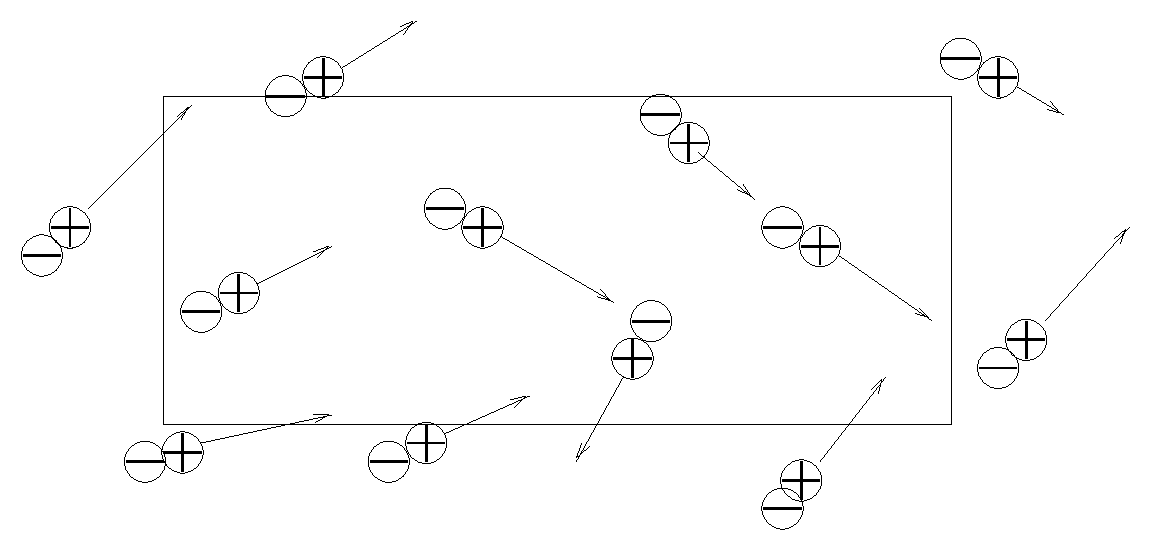
\epsfig{file={../fig/polar},width=6 cm,angle=-90}}   
 \caption{Le vecteur polarisation au point $r$ est la limite du
rapport de la somme des moments dipolaires \'el\'ementaires contenus
dans la bo\^\i te $d\tau$ au volume $d\tau$ lorsque celui-ci tend vers z\'ero.}
 \label{figpolar}
\end{figure}


On peut donc \'ecrire l'\'equation de Maxwell--Gauss 
\begin{equation}
\dive \epsilon_0E=\rho
\end{equation}
sous la forme
\begin{equation}
\dive (\epsilon_0E-P)=0
\end{equation}
Nous avons donc reli\'e les propri\'et\'es microscopiques (les $p$) \`a
la description macroscopique du milieu (par le vecteur
$D=\epsilon_0E-P$). Il reste 
maintenant \`a faire un mod\`ele microscopique de $p$.
Plusieurs mod\`eles peuvent \^etre propos\'es. Un mat\'eriau peut
\^etre constitu\'e de petits dip\^oles tous align\'es dans la m\^eme
direction. D'autes mat\'eriaux (comme l'huile par exemple) sont
constitu\'es de mol\'ecules comportant chacune un moment dipolaire.
Sous l'action d'un champ $E$ ext\'erieur, ces mol\'ecules tendent \`a
s'aligner suivant les lignes de champ de $E$. La moyenne $P$ des $p_i$
donn\'ee par l'\'equation \ref{eqmoyP} qui, lorsque $E$ est nul, est
nulle (\`a cause de la distribution al\'eatoire des moments) devient
non-nulle en pr\'esence d'un champ $E$. Un mod\`ele simple peut \^etre
propos\'e sans rentrer dans les d\'etails de la m\'ecanique quantique
: il consiste \`a dire que $P$ est porportionnel \`a $E$ :
\begin{equation}
P=\chi  E
\end{equation}
o\`u $\chi$ est la polarisabilit\'e du milieu. 
Dans ce cas la relation
\begin{equation}
D=\epsilon_0E-P
\end{equation}
devient :
\begin{equation}
D=(\epsilon_0+\chi )E
\end{equation}
\end{exmp}
\begin{exmp}{\bf Un deuxi\`eme mod\`ele de susceptibilit\'e :}
\'Ecrivons l'\'equation de Vlasov (voir l'\'equation \ref{eqvlasov} et la
r\'ef\'erence \cite{ph:physt:Diu89}).
La fonction $f$ est la densit\'e moyenne de particule et $n_0$
repr\'esente la densit\'e du fond charg\'e positivement.
\begin{equation}\label{vlasdie}
\frac{\partial f}{\partial t}+{v}\partial_x f+\frac{F}{m}\partial_v f= 0
\end{equation}
On suppose que la seule force subie par les particules est la force
\'electrique :
\begin{equation}
\vec{F}=-eE(x,t)
\end{equation}
Les \'equations de Maxwell se mr\'eduisent ici \`a :
\begin{equation}\label{eqmaxsystpart}
\dive E=\rho
\end{equation}
o\`u la charge \'electrique $\rho(x,t)$ est donn\'ee par les fluctuations des
\'electrons autour d'un \'etat de neutralit\'e \'electrique :
\begin{equation}
\rho=-e\int f(x,v,t)dv+en_0
\end{equation}
Lin\'earisons ce syst\`eme d'\'equation par rapport \`a la position
d'\'equilibre suivante :
\begin{eqnarray}
f(x,v,t)&=&f^0(v)+f^1(x,v,t)\nonumber\\
F(x,v,t)&=&0+F_1
\end{eqnarray}
Comme le syst\`eme est \'electriquement neutre (globalement) :
\begin{equation}
\int f^0(v) = n_0
\end{equation}
Par transformation de Fourier en $x$ et $t$ des \'equations \ref{vlasdie} et
\ref{eqmaxsystpart} on a :
\begin{eqnarray}
\epsilon_0 ik \hat{E_1}&=&-e\int \hat{f_1} dv\\
-i\omega \hat{f_1}+ivk\hat{f_1}&=&e\frac{\hat{E_1}}{m} \frac{\partial
\hat{f^0}}{\partial v} 
\end{eqnarray}
En \'eliminant $\hat{f_1}$ du syst\`eme pr\'ec\'edent, nous obtenons :
\begin{equation}
ik\hat{E_1}(\epsilon_0 - \frac{e^2}{km}\int
\frac{1}{vk-\omega}\frac{\partial f}{\partial v})=0
\end{equation}
On peut consid\'erer le premier terme de cette \'equation comme la
divergence d'un vecteur que nous notons $D$ qui s'ecrit $D=\epsilon
*E_1$, o\`u $*$ est la convolution en $x$ et $t$ :
\begin{equation}\label{eqmaxconvol}
\dive(\epsilon *E_1)=0
\end{equation}
Le vecteur $D$ appel\'e
d\'eplacement \'electrique. $\epsilon$ est la susceptibilit\'e du
milieu. 
On a donc ramen\'e l'\'equation de Maxwell \ref{eqmaxsystpart}
d\'ecrivant un syst\`eme de charges ponctuelles dans le vide, \`a
l'\'equation  \ref{eqmaxconvol} qui d\'ecrit le champ dans la
mati\`ere. L'\'equation pr\'ec\'edente nous donne $\epsilon (k,\omega)$
\begin{equation}
\epsilon (k,\omega)=(\epsilon_0 - \frac{e^2}{km}\int
\frac{1}{vk-\omega}\frac{\partial \hat{f}}{\partial v})
\end{equation}
\end{exmp}
\section{\'Elasticit\'e g\'en\'eralis\'ee}\label{secelastigene} 
%%%%%%%%%%%%%%%%%%%%%%%%%%%%
\subsection{Introduction}
%%%%%%%%%%%%%%%%%
Dans cette section nous pr\'esentons le concept d'\'energie \'elastique.
\index{\'elasticit\'e} 
La notion d'\'energie \'elastique permet de d\'eduire facilement des
relations de type ``contrainte--d\'eformation''.\index{relation
contrainte--d\'eformation} 
Ainsi dans une mod\'elisation de la mati\`ere par une m\'ethode de
puissance virtuelle,\index{virtuelle (puissance)} on introduit une
puissance $P$ qui est une 
fonctionelle du d\'eplacement. Consid\'erons le cas particulier d'une
masse $m$ attach\'ee \`a un ressort de constante de couplage $k$. On
rep\`ere la {\bf d\'eformation} du syst\`eme par l'allongement $x$ du
ressort par rapport \`a l'equilibre.
Le {\bf travail virtuel}\index{virtuel (travail)} associ\'e \`a un
d\'eplacement $dx$ est  
\begin{equation}\label{deltWfdx}
\delta W=f.dx
\end{equation}
La quantit\'e $f$ repr\'esente la {\bf contrainte}, ici une force, et
$x$ la d\'eformation. Si la force $f$ est conservative, alors on sait
que le travail \'el\'ementaire (fourni par l'ext\'erieur) est la
diff\'erentielle totale d'une 
fonction \'energie potentielle ou {\bf \'energie interne} $U$ :
\begin{equation}\label{eqdeltaWdU}
\delta W=-dU
\end{equation}
Mais en g\'en\'eral la force $f$ d\'epend de la d\'eformation par une
relation $f(x)$ qui est une {\bf relation contrainte--d\'eformation}.
La mani\`ere la plus naturelle de trouver la relation
contrainte--d\'eformation est la suivante. On cherche l'expression de
$U$ en fonction des d\'eformations en utilisant la physique du
probl\`eme et ses sym\'etries. Dans le cas particulier de
l'oscillateur, on veut que l'\'energie interne ne d\'epende que de $x$,
l'\'ecart \`a l'\'equilibre. 
Si $U$ admet un d\'eveloppement limit\'e en $x=0$, on a l'expression
de $U$ au voisinage de l'\'equilibre :
\begin{equation}
U(x)=a_0+a_1x^1+a_2x^2+O(x^2)
\end{equation}
Comme on veut que $x=0$ soit une position
d'\'equilibre, cela implique que $dU=0$ en $x=0$ ce qui implique que
$a_1$ est nul. La courbe $U(x)$ au voisinage de l'\'equilibre a lors
une forme parabolique (voir figure \ref{figparabe}
\begin{figure}[htb]
 \centerline{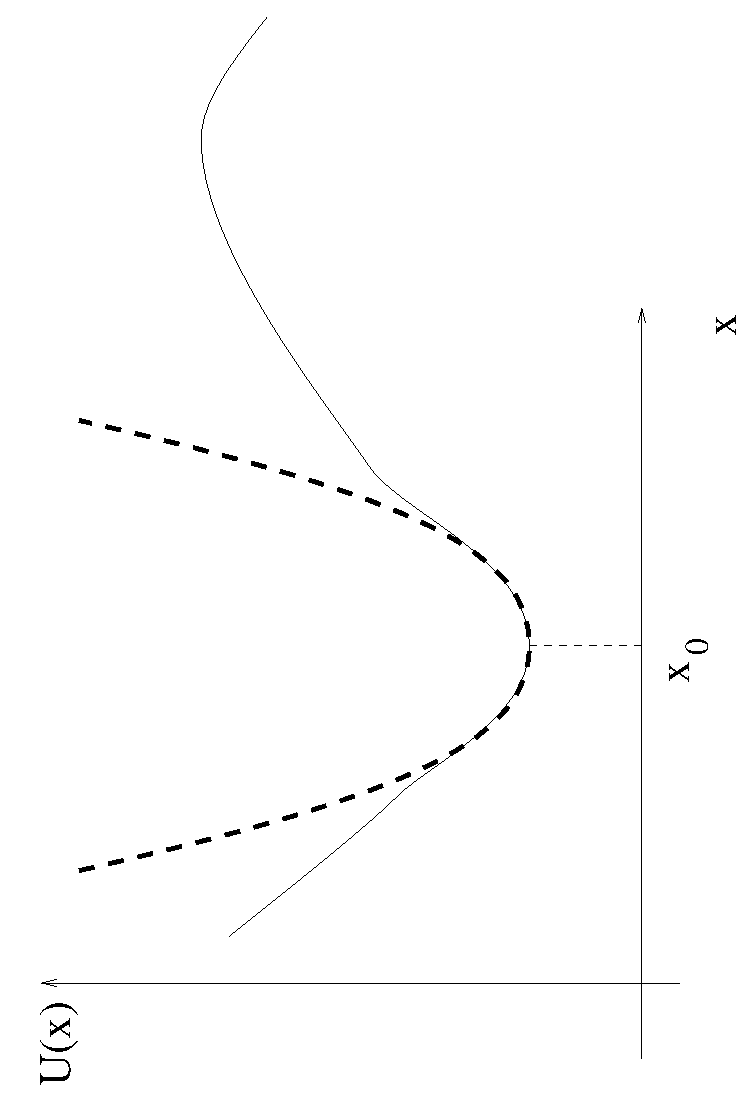
\epsfig{file={../fig/parabe},width=6 cm,angle=-90}}   
 \caption{Au voisinage de l'\'equilibre (stable) $x_0$, l'\'energie
interne $U$ en fonction de l'\'ecart \`a l'\'equilibre pr\'esente un
profil de parabole.}
 \label{figparabe}
\end{figure}
Comme 
\begin{equation}
dU=-fdx
\end{equation}
alors la relation contrainte d\'eformation devient :
\begin{equation}
f=\frac{dU}{dx}
\end{equation}
\subsection{Cha\^\i ne d'oscillateurs}
%%%%%%%%%%%%
Consid\'erons une chaine unidimensionnelle de $N$ oscillateurs coupl\'es par
des constantes $k_{ij}$. Ce syst\`eme est repr\'esent\'e dans la
figure \ref{figchaineosc}. Chaque
oscillateur est rep\'er\'e par son \'ecart par rapport \`a la position
d'\'equilibre  $x_i$. 
Un calcul en utilisant cette fois le formalisme de la relation
fonmdamentale de la dynamique donne :
\begin{equation}
U=\sum\frac{1}{2}k_{ij}(x_i-x_{j-1})^2
\end{equation}
\begin{figure}[htb]
 \centerline{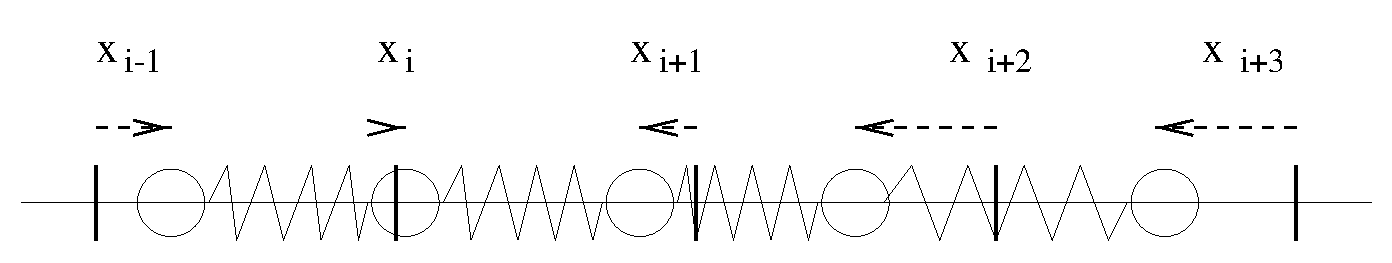
\epsfig{file={../fig/chaineosc},width=6 cm,angle=-90}}   
 \caption{Une cha\^\i ne d'oscillateurs coupl\'es est en particulier
un mod\`ele pour une collection de masses reli\'ees entre elles par
des ressorts parfaits.}
 \label{figchaineosc}
\end{figure}
Un calcul \`a partir de travaux virtuels aurait consist\'e \`a dire :
L'\'energie potentielle \'elastique totale 
est en g\'en\'eral une fonction $U(x_1,\dots, x_N)$. 
Elle est une diff\'erentielle totale car on suppose la force
conservative\footnote{C'est cette supposition qui est la plus difficile \`a
d\'emontrer dans les th\'eories sur l'\'elasticitit\'e comme on le vera
\`a la section suivante}. Donc \`a l'\'equilibre\index{\'equilibre} :
\begin{equation}
dU=0
\end{equation}
Si $U$ admet un developpement limit\'e :
\begin{equation}\label{eqdevliUch}
U(x_1=0,\dots x_N=0)=a+a_i x_i+a_{ij}x_ix_j+O(x^2)
\end{equation}
Dans cette derni\`ere \'equation, on a utilis\'e la convention de
sommation de l'indice r\'ep\'et\'e.
En d\'efinissant la diff\'erentielle de l'\'energie interne comme :
\begin{equation}
dU=f_i dx_i
\end{equation}
on a :
\begin{equation}
f_i=\frac{\partial U}{\partial x_i}
\end{equation}
donc, en utilisant l'expression \ref{eqdevliUch} de $U$ :
\begin{equation}
f_i=a_{ij}x_j
\end{equation}
Mais comme ici l'interaction entre les masses ne se fait qu'entre plus
proches voisins, les variables $x_i$ ne sont pas les bonnes variables
thermodynamiques. Choisissons comme variables thermodynamique les
\begin{equation}
\epsilon_i=x_i-x_{i-1}.
\end{equation}
La diff\'erentielle de $U$ devient :
\begin{equation}
dU=F_id\epsilon_i
\end{equation}
En supposant que $U$ admet un d\'evelopement limit\'e autour de la
position d'\'equilibre
\begin{equation}
U=b+b_i\epsilon_i+b_{ij}\epsilon_i\epsilon_j+O(\epsilon^2)
\end{equation}
et que $dU=0$ \`a l'equilibre, alors on a :
\begin{equation}
F_i=b_{ij}\epsilon_j
\end{equation}
Comme l'interaction est entre plus proches voisins :
\begin{equation}
b_{ij}=0 {\rm\ si\ } i\neq j\pm 1
\end{equation}
Donc 
\begin{equation}
F_i=b_{ii}\epsilon_i+b_{ii+1}\epsilon_{i+1}
\end{equation}
ce qui correspond bien \`a l'expression de la force appliqu\'ee \`a la
masse $i$ :
\begin{equation}
F_i=-k(x_{i}-x_{i-1})-k(x_{i+1}-x_{i})
\end{equation}
si on pose $k=-b_{ii}=-b_{ii+1}$.
\subsection{Mat\'eriau \'elastique tridimensionel}\label{secmaterelast}
%%%%%%%%%%%
Consid\'erons un syst\`eme $S_X$ d\'eformation de $S_0$ o\`u la
position de 
chaque particule de $S_0$ est rep\'er\'ee par $a$ et celle de $S_X$ est
rep\'er\'e par $x$ avec :
\begin{equation}
x=a+X
\end{equation}
\begin{rem}
Un tel mod\`ele permet de d\'ecrire par exemple un fluide ou un solide.
\end{rem}
Consid\'erons le cas o\`u $X$ est toujours ''petit''. Nous trouvons
alors dans le cadre de 
l'hypoth\`ese des petites perturbations (HPP).
On cherche en g\'en\'eral $U$ sous la forme 
 $U(X)$.
\begin{defn}
On appelle tenseur de d\'eformation HPP la partie sym\'etrique du tenseur
gradient de $X$.
\begin{equation}
\epsilon_{ij}=\frac{1}{2}(X_{i,j}-X_{j,i})
\end{equation}
\end{defn}
\`A la section \ref{secpuisvirtu} nous avons vu que la puissance des
efforts int\'erieurs  admissibles pour ce type de probl\`eme est :
\begin{equation}
P_i=\int K_{ij}^s u_{i,j}^s
\end{equation}
avec
\begin{equation}
dU=-P_idt
\end{equation}
Le tenseur $u_{i,j}^s$ est appel\'e tenseur taux de d\'eformation.
C'est la partie sym\'etrique du tenseur $u_{i,j}$. On montre
\cite{ph:fluid:Germain80} que dans le cadre des hypoth\`eses HPP, le tenseur taux
de d\'eformation est 
simplement la d\'eriv\'ee du tenseur de d\'eformation HPP par rapport au temps
:
\begin{equation}
u_{i,j}^s=\frac{d\epsilon_{ij}}{dt}
\end{equation}
On a donc 
\begin{equation}\label{dukij}
dU=-\int K_{ij}^s d\epsilon_{ij}d\tau.
\end{equation}
On cherche donc $U$ sous la forme $U(\epsilon_{ij})$.
Plus pr\'ecis\'ement, on cherche $U$ sous la forme :
\begin{equation}
U=\int \rho e_l d\tau
\end{equation}
o\`u $e_l$ est une densit\'e d'\'energie interne avec\footnote{%%%
ce qui d\'ecoule du fait que  $U$ ne d\'epende que de
$\epsilon_{ij}$.} %%%%%%%%%%%%%%%%%%%%%%%
dont le d\'evelopement limit\'e autour de la position d'\'equilibre
est :
\begin{equation}\label{eqrhoel}
\rho e_l=a+a_{ij}\epsilon_{ij}+a_{ijkl}\epsilon_{ij}\epsilon_{kl}
\end{equation}
Nous avons\footnote{\label{footdensi}En effet :%%%%%%%%%% 
\begin{equation}
\frac{d}{dt}U=\frac{d}{dt}\int \rho e_l d\tau
\end{equation}
et d'apr\`es les propri\'et\'es de la d\'eriv\'ee particulaire :
\begin{equation}
\frac{d}{dt}\int \rho e_l d\tau=\int\frac{d}{dt}( \rho e_l d\tau)
\end{equation}
Or :
\begin{equation}
\frac{d}{dt} (\rho e_ld\tau)=e_l\frac{d}{dt} (\rho d\tau) + \rho
d\tau\frac{d}{dt}e_l 
\end{equation}
D'apr\`es le principe de conservation de la masse :
\begin{equation}
\frac{d}{dt} \rho=0
\end{equation}
}%%%%%%%%%%%%%%%%%%%%%%%%%%%%
\begin{equation}\label{eqdudt}
\frac{dU}{dt}=\int \rho (\frac{d}{dt}e_l) d\tau
\end{equation}
Donc
\begin{equation}
dU=\int \rho de_l d\tau
\end{equation}
En utilisant l'expression \ref{eqrhoel} de $e_l$ et en supposant que
$dU$ est nul \`a l'equilibre, on a :
\begin{equation}
dU=\int \rho  [a_{ijkl}\epsilon_{ij}d\epsilon_{kl}+
a_{ijkl}d\epsilon_{ij}\epsilon_{kl}]d\tau 
\end{equation}
soit :
\begin{equation}
dU=\int \rho  b_{ijkl}\epsilon_{kl}d\epsilon_{ij}d\tau
\end{equation}
avec $b_{ijkl}=a_{ijkl}+a_{klij}$. Par identification avec
\ref{dukij} on obtient la relation d\'eformation--contrainte :
\begin{equation}
K_{ij}^s=b_{ijkl}\epsilon_{kl}
\end{equation}
Il s'agit d'une loi de Hooke g\'en\'eralis\'ee. Les $b_{ijkl}$ sont
les coefficients d'\'elasticit\'e. 
\begin{rem}
Le calcul de la note de bas de page \ref{footdensi} montre que les calculs
faits \`a la 
section pr\'ec\'edente \ref{secchampdslamat}
devraient en toute rigueur porter sur les densit\'es volumique d'\'energie.
\end{rem}

\subsection{Mat\'eriau n\'ematique}\label{secenernema}
%%%%%%%%%%%
Un mat\'eriau n\'ematique\index{n\'ematique} est un mat\'eriau
\cite{ph:liqcr:DeGennes74} dont 
l'\'etat est caract\'eris\'e par un champ\footnote{Il existe aussi de
mat\'eriaux dits smectique dont l'\'etat est caract\'eris\'e par une
fonction $u(x,y)$} de vecteurs $n$. ce champ est reli\'e \`a
l'orientation des mol\'ecules du mat\'eriau (voir la figure
\ref{figchampnema})
\begin{figure}[htb]
 \centerline{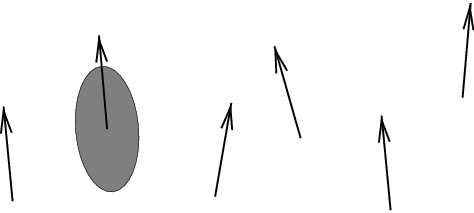
\epsfig{file={../fig/champnema},width=6 cm,angle=-90}}   
 \caption{L'orientation de chaque mol\'ecule du n\'ematique est
d\'ecrite par un vecteur $n$. Dans un mod\`ele continu, on a un champ
de vecteur $n$. L'\'energie interne du n\'ematique est une fonction du
champ de vecteurs $n$ et de ses d\'eriv\'ees partielles.}
 \label{figchampnema}
\end{figure}
\begin{equation}
U=\int K_{ij} \partial_i n_j
\end{equation}
o\`u $K_{ij}$ est un tenseur du second ordre d\'ependant de $r$.
\'Etudions les sym\'etries de $U$.
La fonctionelle $U$ doit \^etre invariante par rotation :
\begin{equation}
U(\partial_i n_j)=U(R_{ik}R_{jl}\partial_k n_l)
\end{equation}
o\`u $R_{mn}$ sont des transformations orthogonales (rotations).
On a donc la condition :
\begin{equation}
K_{ij}=R_{ik}R_{jl}K_{kl}
\end{equation}
Autrement dit $K_{ij}$ doit \^etre isotrope.
On sait que le seul tenseur de rang 2 qui est isotrope 
dans un espace \`a 3 dimensions est $\delta_{ij}$ 
c'est \`a dire l'identit\'e.
Donc $U$ comporte un terme de la forme
\begin{equation}
k_0\dive n
\end{equation}
L'\'energie de la distorsion est ind\'ependante du sens de $n$.
Donc $U(n)=U(-n)$.
Donc $k_0=0$.
Cherchons une forme plus g\'en\'erale pour $U$. Permettons a 
$K_{ij}$ d'\^etre une fonction de $n$.
La condition d'invariance par la transformation $n$ donne
$-n$ implique que $K_{ij}$ est une fonction impaire de $n$.
\begin{equation}
K_{ij}(-n)=-K_{ij}(n)
\end{equation}
La fonction impaire la plus g\'en\'erale de $n$ qui tient compte 
des termes lin\'eaires en $n$ est :
\begin{equation}
K_{ij}=L_{ijk}n_k
\end{equation}
La condition d'invariance par rotation implique maintenant 
\begin{equation}
L_{ijk}=R_{il}R_{jm}R_{kn}L_{lmn}
\end{equation}
pour toute rotation. On sait qu'il n'existe
pas de tenseur isotrope de rang 3, mais il existe un pseudo-tenseur
isotrope de rang trois, c'est le tenseur signature des perumtations $e_{jkl}$
(voir l'annexe \ref{secformultens}).
Donc $U$ comporte un terme de la forme :
\begin{equation}
U=k_1n\rot n.
\end{equation}
Le tenseur $e_{jkl}$ est invariant par toute transformation orthogonale
positive mais dans une changement d'axe du type :
$x\rightarrow -x$, $y\rightarrow -y$, $z\rightarrow -z$, il change 
de signe. Ceci n'est pas autoris\'e pour les n\'ematiques\footnote{%%%%%
 C'est autoris\'e
pour certains mat\'eriaux comme les cholest\'eriques. }, donc $k_1=0$.%%%%%%%%%%%%%%%
Les conditions de  sym\'etries ont \'elimin\'e tous les termes en
$\partial_i n_j$. 

On peut montrer que si l'on envisage les termes en $\partial_i n_j\partial_k
n_l$ alors des consid\'erations de sym\'etries du m\^ eme type que celle vues
plus haut impliquent que les seuls termes du second ordre ({\it i.e} en
$\partial_i n_j\partial_kn_l$) que $U$ peut contenir sont du type $(\dive
n)^2$, $(n.\rot n)^2$ et $(n \wedge \rot n)^2$. Notre mod\`ele final pour
l'\'energie $U$ d'un n\'ematique est donc :
\begin{equation}
U=K_1 (\dive n)^2+K_2 (n.\rot n)^2+K_3(n \wedge \rot n)^2
\end{equation}



\section{Autres ph\'enom\`enes}
%%%%%%%%%%%%%%%%%%%%%%%
\subsection{Piezo\'electricit\'e }
%%%%%%%%%%%%%%%%%
Dans l'\'etude de la {\bf piezo\'electricit\'e }
\cite{ph:elect:LandauEle}, on\index{piezo\'electricit\'e} 
choisit pour $ \sigma_{ij}$ :
\begin{equation}
\sigma_{ij}=\lambda_{ijkl}u_{kl}+\gamma_{ijk}E_k
\end{equation}
$\gamma_{ijk}$ provient d'un couplage entre les variables champ
\'electrique $E_i$ et les variables d\'eformation dans l'expression de F :
\begin{equation}
F=F_0+\epsilon_{ij}E_iE_j+\frac{1}{2}\lambda_{ijkl}u_{ij}u_{kl}+
\gamma_{ijk}E_iu_{jk} 
\end{equation}
et l'expression de $D_i$ devient :
\begin{equation}
D_i=\left.\frac{\partial F}{\partial E_i}\right)_{ufix\acute e,Tfix\acute e}
\end{equation}
soit :
\begin{equation}
D_i=\epsilon_{ij}E_j+\gamma_{ijk}u_{jk}
\end{equation}

\subsection{Viscosit\'e}
%%%%%%%%%%%%%%%%%%%
On dit qu'il y a viscosit\'e\index{viscosit\'e} d\`es que le tenseur
de contrainte d\'epend des vitesses de d\'eformation.
Dans la th\'eorie de {\bf la visco\'elasticit\'e
lin\'eaire}\cite{ma:equad:Dautray1,ma:equad:Duvaut72}, on peut prendre comme
relation contrainte--d\'eformation :
\begin{equation}
\sigma_{ij}=a_{ijkl}u_{kl}+b_{ijkl}\frac{\partial u_{kl}}{\partial t}
\end{equation}
On parle alors de {\bf mat\'eriaux \`a m\'emoire courte}
puisque\index{m\'emoire} 
l'\'etat de contrainte \`a l'instant $t$ ne d\'epend que de la
d\'eformation \`a cet instant et aux instants imm\'ediatement
pr\'ec\'edents. Les tenseurs $a$ et $b$ joue respectivement le r\^ole de
coefficients d'\'elasticit\'e et de viscosit\'e. 
Si on prend comme
relation contrainte--d\'eformation une relation du type suivant :
\begin{equation}\label{eqmatmem}
\sigma_{ij}=a_{ijkl}u_{kl}+\int_0^tb_{ijkl}(t-s)u_{kl}(s)ds
\end{equation}
alors le mat\'eriau est dit {\bf \`a m\'emoire longue} car l'\'etat des
contraintes d\'epend de la d\'eformation \`a l'instant $t$ mais aussi
des d\'eformations aux instants ant\'erieurs \`a $t$.
Le premier terme du second membre repr\'esente un effet \'elastique
instantan\'e. Le deuxi\`eme membre rend compte des effets de m\'emoire.
\begin{rem}
Ces mat\'eriaux\cite{ma:equad:Duvaut72} font partie d'une classe particuli\`ere de
mat\'eriaux de {\it type taux }pour lesquels on a une relation
lin\'eaire entre les d\'eriv\'ees par rapport au temps des tenseurs de
d\'eformation et de contraintes. On a donc :
\begin{equation}
\sigma_{ij}(t)+a^1_{ijkl}\frac{\partial \sigma_{kl}(t)}{\partial
t}+\dots+a^{n_1}_{ijkl}\frac{\partial^{n_1} \sigma_{kl}(t)}{\partial
t^{n_1}} 
\end{equation}
\begin{equation}
=b^0_{ijkl}u_{kl}(t)+b^1_{ijkl}\frac{\partial u_{kl}(t)}{\partial
t}+\dots+b^{n_2}_{ijkl}\frac{\partial^{n_2} u_{kl}(t)}{\partial
t^{n_2}} 
\end{equation}
Par transformation de Laplace on peut montrer qu'il est \'equivalent de
consid\'erer la loi :
\begin{equation}
\sigma_{ij}(t)=A^0_{ijkl}u_{kl}(t)+A^1_{ijkl}\frac{\partial
u_{kl}(t)}{\partial t}+\dots+A^{N}_{ijkl}\frac{\partial^{N}
u_{kl}(t)}{\partial t^{N}}+b_{ijkl}*u_{kl}(t) 
\end{equation}
o\`u $N=n_2-n_1$ et o\`u $b(t)$ est une fonction r\'eguli\`ere.
\end{rem}
\begin{rem}
Si on se place dans le cadre des distributions on peut consid\'erer les
d\'erivations comme des convolutions par des d\'eriv\'ees de la distribution
de Dirac. Par exemple, la d\'erivation par rapport au temps peut
s'exprimer par la convolution.
par $\delta '(t)$. On rentre donc en fait dans le cadre g\'en\'eral de
la formule \ref{eqmatmem}.
\end{rem}

\section{Exercices}
%%%%%%%%%%%%%%%%%

\begin{exo}
Trouver l'\'equation d'\'evolution pour une corde tendue entre deux murs.
\end{exo}

\begin{exo}
Trouver l'\'equation de propagation du son dans une colonne d'air. Pour
obtenir l'\'equation de la dynamique, on utilisera une des m\'ethode vues au
chapitre pr\'ec\'edent (loi de conservation ou pricipe des puissances
virtuelles). Pour obtenir la relation contrainte--d\'eformation, on supposera
que le gaz subit des tranformations adiabatiques, {\it i.e.}
$pV^{\gamma}$=constante, o\`u $p$ est la pression du gaz, $V$ le volume de
l'air et $\gamma$ une constante.
\end{exo}

\begin{exo}
Donner l'expression de l'\'energie de d\'eformation d'un smectique (voir la
section \ref{secristliquides} pour la description d'un smectique) dont
l'\'etat de la i--\`eme couche est d\'ecrite par une surface $u_i(x,y)$,
\end{exo}

\begin{exo}
Consid\'erons un mat\'eriau lin\'eaire, homog\`ene, isotrope. 
La susceptibilit\'e $\epsilon$ introduite \`a la section \ref{secchampdslamat}
permet pour de tel mat\'eriaux de donner par simple convolution $D$ \`a partir
de $E$ :
\begin{equation}\label{eqexsusc}
D=\epsilon * E.
\end{equation}
o\`u $*$ repr\'esente une convolution temporelle. Pour ob\'eir au principe de
causalit\'e, la distribution $\epsilon$ se doit d'\^etre \`a support
positif. En effet, $D$ ne peut d\'ependre des valeurs prises par $E$ dans le
futur. Sachant que la transform\'ee de Fourier de la fonction signe de $t$ est
$C.V_p(1/x)$ o\`u $C$ est une constante de normalisation et $V_p(1/X)$ la
distribution valeur principale de $1/x$, donner les relations entre les
parties r\'eelles et imaginaire de la transform\'e de Fourier de la
distribution $\epsilon$.  ces relations sont connues en optique sous le nom de
relations de {\bf Krammers--Kr\"onig}.
\end{exo}

\appendix
%%%%%%%%%%%%%%%%%%%
%%%%%%%%%%%%%%%%%%%%%%
\chapter{Distributions}
%%%%%%%%%%%%%%%%%%%%%%%
\section{Distributions de L. Schwartz}
%%%%%%%%%
Les distributions\index{distribution} permettent de d\'ecrire de
mani\`ere \'el\'egante
et synth\'etique bien des ph\'enom\`enes physiques. Ainsi elle
permettent de mod\'eliser des charges ponctuelles, des dip\^oles.
Elles permettent aussi de g\'en\'eraliser la notion de d\'erivation
\`a des fonctions qui ne sont pas continues.
\begin{defn}
Un espace fonctionnel est un ensemble ${\cal F}$ de fonctions ayant
une structure d'espace vectoriel.
\end{defn}
\begin{defn}Une fonctionnelle $T$ de ${\cal F}$ est une application de
${\cal F}$ dans $C$.
\end{defn}
On d\'esigne par $<T|\phi>$ le nombre associ\'e \`a la fonction $\phi$ par la
fonctionnelle $T$.
\begin{defn}
Une fonctionnelle $T$ est lin\'eaire si quelles que soient $\phi_1$ et
$\phi_2$ de ${\cal F}$ et les nombres complexes $\lambda_1$ et
$\lambda_2$ :
\begin{equation}
<T|\lambda_1\phi_1+\lambda_2\phi_2> =
\lambda_1<T|\phi_1>+\lambda_2<T|\phi_2> 
\end{equation}
\end{defn}
\begin{defn}
L'espace ${\cal D}$ est l'espace vectoriel des fonctions
ind\'efiniment d\'erivables \`a support born\'e.
\end{defn}
\begin{defn}
Les distributions de L. Schwartz sont les fonctionnelles lin\'eaires
continues sur ${\cal D}$, donc des \'el\'ements du dual ${\cal D}'$ de
${\cal D}$.
\end{defn}
\begin{defn}
Une fonction est dite localement sommable si elle est int\'egrable au
sens de Lebesgue sur tout intervalle born\'e.
\end{defn}
\begin{defn}
\`A toute fonction localement sommable $f$ on peut associer une
distribution $T_f$ d\'efinie par :
\begin{equation}
\forall \phi \in {\cal D},\ <T_f|\phi>=\int f(x)\phi(x)dx
\end{equation}
\end{defn}
\begin{defn}
La distribution de Dirac,\index{distribution de Dirac}\index{Dirac
(distribution de)} not\'ee $\delta$ est d\'efinie par :
\begin{equation}
\forall \phi \in {\cal D},\ <\delta|\phi>=\phi(0)
\end{equation}
\end{defn}
\begin{rem}
Le physicien utilise souvent la notation int\'egrale (incorrecte)
\begin{equation}
\int \delta(x)\phi(x)dx=\phi(0)
\end{equation}
pour d\'ecrire l'action de $\delta$ sur $\phi$.
\end{rem}
\section{Limites au sens des distribution}
%%%%%%%%%%%%%%%%%%%%%%%%%%%%%%%%
\begin{defn}
Soit $T_\alpha$ une famille de distributions d\'ependant d'un
param\`etre $\alpha$ (non n\'ec\'essairement entier). On dit que
$T_\alpha$ admet pour limite la distribution $T$ quand $\alpha$ tend
vers $\lambda$ si :
\begin{equation}
\forall \phi \in {\cal D},
\lim_{\alpha\rightarrow\lambda}<T_\alpha,\phi>=<T,\phi> 
\end{equation}
\end{defn}
En particulier, on d\'emontre que les distributions associ\'ees aux
fonctions $f_\alpha$ v\'erifiant :
\begin{equation}
f_\alpha(x)\geq 0
\end{equation}
\begin{equation}
\int f_\alpha(x)dx=1
\end{equation}
\begin{equation}
\forall a\geq 0,
\lim_{\alpha\rightarrow\infty}\int_{|x|>a}f_\alpha(x)dx=0 
\end{equation}
convergent vers la distribution de Dirac.
\begin{figure}[htb]
 \centerline{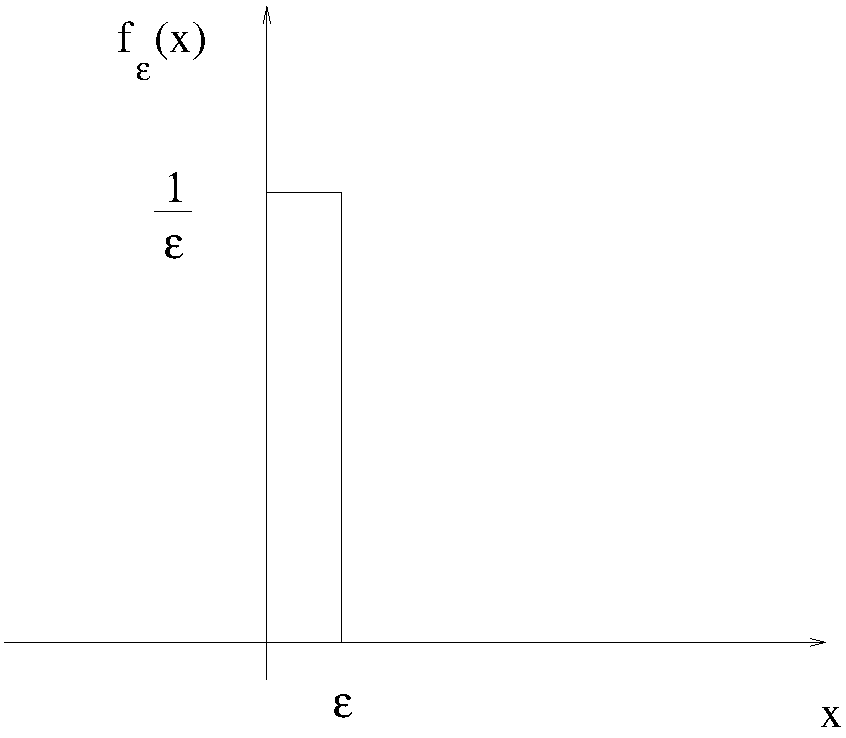
\epsfig{file={../fig/dirac},width=6 cm,angle=-90}}   
 \caption{La famille de fonctions $f_\epsilon$ o\`u $f_\epsilon$ vaut
$1/\epsilon$ sur l'intervalle $[0,\epsilon]$ et z\'ero ailleurs
converge vers la distribution de Dirac quand $epsilon$ tend vers
z\'ero.  }
 \label{figdirac}
\end{figure}
La figure \ref{figdirac} repr\'esente un exemple d'une telle famille
de fonctions.
\section{D\'eriv\'ee au sens des distributions}
%%%%%%%%%%%%%%%
La d\'eriv\'ee\index{d\'eriv\'ee au sens des ditributions} au sens
usuel des fonctions n'est pas d\'efinie pour 
les fonctions non-continues.
La th\'eorie des distributions nous permet en particulier de
g\'en\'eraliser la notion de d\'eriv\'ee \`a des fonctions non
continues.
\begin{defn}
La d\'eriv\'ee d'une distribution $T$ est la distribution $T'$
d\'efinie par :
\begin{equation}
\forall \phi \in {\cal D},\ <T'|\phi>=-<T|\phi'>
\end{equation}
\end{defn}
\begin{defn}
Soit $f$ une fonction sommable. Supposons que $f$ soit
discontinue en $N$ points $a_i$, et notons
$\sigma_{a_i}=f(a_i^+)-f(a_i^-)$ le saut de $f$ en $a_i$.
Supposons que $f'$ soit localement sommable et presque partout
d\'efinie. Elle d\'efinit alors une distribution $T_{f'}$.
La d\'eriv\'ee $(T_f)'$ de la distribution associ\'ee \`a $f$ est :
\begin{equation}
(T_f)'=T_{f'}+\sum \sigma_{a_i} \delta_{a_i}
\end{equation}
On dit que la d\'eriv\'ee au sens des distributions est \'egale \`a la
d\'eriv\'ee sans pr\'ecaution augment\'ee de la distribution de Dirac
multipli\'ee par le saut de $f$. On note :
\begin{equation}
f'=\{f'\}+\sum \sigma_{a_i} \delta_{a_i}
\end{equation}
\end{defn}
Nous allons voir quelques applications de la th\'eorie des
distributions apr\`es avoir ennonc\'e le th\'eor\`eme fondamental suivant :
\begin{thm}
La relation fondamentale de la dynamique et les lois de Maxwell sont
vraies au sens des distributions.
\end{thm}
Ce th\'eor\`eme permet de d\'emontr\'ee facilement la th\'eorie des
percussions en m\'ecanique et les relation de passages en
\'electromagn\'etisme \cite{ph:elect:Petit89}. 
\section{Distributions en physique}
%%%%%%%%%%%%%%%%
\subsection{Distributions de plusieurs variables}\label{secdisplu}
%%%%%%%%%%%%%%%%%%%%%%%%%%%%%
En utilisant les d\'eriv\'ees sans pr\'ecaution, on peut \'ecrire l'action des
op\'erateurs diff\'erentiels, au sens des distributions, dans le cas o\`u les
quantit\'es sur lesquelles ils s'appliquent pr\'esentent une discontinuit\'e
sur une surface $S$ :
\begin{equation}
\frac{\partial f}{\partial x_i}=\{\frac{\partial f}{\partial
x_i}\}+n_i\sigma_f \delta_S
\end{equation}
\begin{equation}
\grad f=\{\grad f\}+n \sigma_f \delta_S
\end{equation}
\begin{equation}
\dive a=\{ \dive f\}+n \sigma_a \delta_S
\end{equation}
\begin{equation}
\rot a = \{\rot f\}+n\wedge \sigma_a \delta_S
\end{equation}
o\`u $f$ est une fonction scalaire, $a$ une fonction vectorielle, $\sigma$
repr\'esente le saut de $a$ ou $f$ \`a travers la surface, et $\delta_S$, la
distribution de Dirac surfacique.
Ces formules permettent de retrouver les formules de Green introduites
pour les tenseurs.

\section{Circuits \'electriques}
%%%%%%%%%%%
Nous avons vu que les \'equations de Maxwell sont vraies au sens des
distributions.  
Les distributions nous permettent de justifier certaines affirmations
parfois non-justifi\'ees dans les cours d'\'electricit\'e.
Consid\'erons l'\'equation :
\begin{equation}
U(t)=L\frac{di}{dt}+Ri
\end{equation}
Cette \'equation implique que m\^eme si $U$ est discontinue, $i$ est
continue. En effet, si $i$ est discontinue, la d\'eriv\'ee
$\frac{di}{dt}$ ferait appara\^\i tre une distribution de Dirac dans
le second membre.
Consid\'erons l'\'equation :
\begin{equation}
i=\frac{dq}{dt}
\end{equation}
Cette \'equation implique que $q(t)$ est continue m\^eme si $i$
discontinue.
\section{M\'ecanique des fluides}
%%%%%%%%%%%%%%%%%%%%%
Les lois de conservation sont des lois vraies au sens des
distributions. En utilisant la d\'erivation au sens des distributions
on obtient imm\'ediatement les relations dites de ``discontinuit\'e''
\cite{ph:fluid:Germain80}.
Envisageons le cas de la conservation de la masse :
\begin{equation}
\frac{partial \rho}{\partial t}+\dive(\rho \vec{u})=0
\end{equation}
Comme 
\begin{equation}
\dive \rho {u}=\{\dive \rho {u}\}+\sigma_{\rho u},
\end{equation}
le saut $\sigma_{\rho u}$ doit \^etre nul sur une surface de discontinuit\'e.

\section{\'Electromagn\'etisme}
%%%%%%%%%%%%%%%%%%%%%%%
Les lois fondamentales de l'\'electromagn\'etisme sont les \'equations
de Maxwell que nous rappelons ici :\index{relations de passage}
\begin{equation}
\rot E=-\frac{\partial B}{\partial t}
\end{equation}
\begin{equation}
\rot H=j+\frac{\partial D}{\partial t}
\end{equation}
\begin{equation}
\dive D=\rho
\end{equation}
\begin{equation}
\dive B=0
\end{equation}
Dans les livres sur l'\'electromagn\'etisme, un chapitre est souvent
consacr\'e \`a l'\'etude des conditions aux limites et conditions de
passages. Si l'on suppose que les distributions de charges autoris\'ees
sont de la forme :
\begin{equation}
\rho=\rho_v+\rho_s
\end{equation}
et
\begin{equation}
j=j_v+j_s
\end{equation}
alors en utilisant les formules de la section
\ref{secdisplu}, on obtient les relations de passage 
\begin{eqnarray}
n_{12}\wedge(E_2-E_1)&=&0\\
n_{12}\wedge(H_2-H_1)&=&j_s\\
n_{12}(D_2-D_1)&=&\rho_s\\
n_{12}(B_2-B_1)&=&0
\end{eqnarray}
o\`u l'on a identifi\'e les termes en $\delta_S$
(voir \cite{ma:distr:Petit91}).
\chapter{Tenseurs}\label{chaptens}
%%%%%%%%%%%%%%%%%
\section{Introduction}
%%%%%%%%%%%%%%%%%%%%
Nous repr\'esentons par $x^i$ les composantes d'un vecteur $X\in E$
dans une \index{tenseur}
base $e_i$ de $E$. Dans une autre base $e'_i$ de $E$ le vecteur $X$ a
pour composantes $x'^i$. La formule de changement de base est :
\begin{equation}
x^i=\omega^i_kx'^k
\end{equation}
o\`u l'on a utilis\'e la convention d'Einstein ou de l'indice r\'ep\'et\'e.
Une forme bilin\'eaire $a(x,y)$ sur $E$ est un tenseur du second ordre
deux fois covariant.\index{covariance}  Le tenseur $a$ est d\'efini
par ses composantes $a_{kl}$ telles que : 
\begin{equation}
a(x,y)=a_{kl}x^ky^l
\end{equation}
Le tenseur $a$ est donc souvent not\'e simplement $a_{kl}$. Le tenseur $a$ est
une 
\'el\'ement d'un espace vectoriel not\'e $E^*\otimes E^*$. Une base de
$E^*\otimes E^*$ est $e^i\otimes e^j$.
Dans une base $e'^i\otimes e'^j$
le tenseur $a$ a pour composantes les $a'_{kl}$ d\'efinis par :
\begin{equation}
a'_{ij}=\omega^k_i\omega^l_j a_{kl}
\end{equation}
On d\'efinit de m\^eme des tenseurs du $n^{\grave eme}$ ordre $n$ fois
covariants comme des $n$--formes lin\'eaires sur $E$.
Un tenseur du second ordre deux fois contravariant est une forme
bilin\'eaire sur $E^*$. De m\^eme, on d\'efinit des tenseurs du
$n^{\grave eme}$ ordre $n$ fois contravariants comme de $n$ 
formes lin\'eaires sur $E^*$. Des tenseurs mixtes peuvent aussi \^etre
d\'efini. Par exemple un tenseur du second ordre une fois covariant
et une fois contravariant est d\'efini comme une forme bilin\'eaire
sur $E\times E^*$ et est not\'e $a^i_j$.
Un exposant repr\'esente la contravariance, un indice la covariance. 
\begin{rem}
Un vecteur peut \^etre consid\'er\'e comme un tenseur de rang 1 et un
scalaire, comme un tenseur de rang z\'ero.
\end{rem}
Le produit d'un tenseur $a$ de rang $p$ par un tenseur $b$ de rang $q$
est un 
tenseur $c$ de rang $p+q$. Par exemple si $a$ est $a_{ij}$ et $b$ est
$b^k_l$, alors $c$ est $c_{ijl}^k=a_{ij}b^k_l$.
On appelle contraction d'un tenseur $a_{ijk\dots}$ par rapport aux
deux indices $i$ et $j$ le tenseur $A_{k\dots}=\sum_ia_{iik\dots}$
\cite{ma:tense:Brillouin38,ma:tense:Bass64}.
Lorsque l'espace $E$ est m\'etrique, on peut transformer un tenseur
contravariant en un tenseur covariant.
Si l'on consid\`ere la repr\'esentation des tenseurs uniquement dans
des bases orthonorm\'ees, alors la distinction entre co-- et
contravariance n'a plus lieu d'\^etre. Ce sont ces tenseurs que nous
consid\'erons par la suite. Un tenseur de rang $n$ sera not\'e par
$n$ indices (et z\'ero exposant).
\begin{defn}
Un tenseur de rang deux est sym\'etrique si $a_{ij}=a_{ji}$.
\end{defn}
\begin{defn}
Un tenseur de rang deux est antisym\'etrique si $a_{ij}=-a_{ji}$.
\end{defn}
\begin{exmp}
Le produit vectoriel est un tenseur de rang deux antisym\'etrique.
\end{exmp}
\begin{rem}
On d\'efinit ausi des pseudo--tenseurs \cite{ma:tense:Bass64} par la relation
de changement 
de base (pour un tenseur de rang deux) :
\begin{equation}
a'_{ij}=det(\omega)\omega^k_i\omega^l_j a_{kl}
\end{equation}
o\`u $det(\omega)$ est le d\'eterminant de la transformation
 $\omega$.
\end{rem}
\section{Sym\'etries}
%%%%%%%%%%%%%%%%%%%%
Soit $a_{ijk}$ un tenseur de rang trois. Consid\'erons le tenseur 
\begin{equation}
X_{ijk}=x_ix_jx_k
\end{equation}
Formons la densit\'e 
\begin{equation}
\phi=a_{ijk}X_{ijk}
\end{equation}
$\phi$ se conserve par changement de base\footnote{%
Un op\'erateur unitaire conserve le produit scalaire voir MQ}
Donc si par sym\'etrie 
\begin{equation}
Ra_{ijk}=a_{ijk}
\end{equation}
alors
\begin{equation}
RX_{ijk}=X_{ijk}
\end{equation}
Autremenent dit "X se transforme comme
$a$"\cite{ma:tense:Bass64,ma:tense:Brillouin38} 
\begin{exmp} : {\bf piezzo-\'electricit\'e.}
Il existe une relation lin\'eaire entre le tenseur de d\'eformation
$e_{ij}$ et le champ electique $h_k$
\begin{equation}
e_{ij}=a_{ijk}h_k
\end{equation}
$a_{ijk}$ est apellle tenseur piezzo-\'electrique.
Montrons que les consid\'erations pr\'ec\'edentes nous permettent d'obtenir des r\'esultats comme le suivant :
\begin{thm}
Si le cristal poss\`ede un centre alors il ne peut avoir des propri\'et\'es piezzo-electriques.
\end{thm}
\begin{pf}
\begin{equation}
R(x_ix_jx_k)=(-1)^3x_ix_jx_k
\end{equation}
or si 
\begin{equation}
Ra_{ijk}=a_{ijk}
\end{equation}
alors 
\begin{equation}
a_{ijk}=-a_{ijk}
\end{equation}
ce qui prouve le th\'eor\`eme.
\end{pf}
\end{exmp}
\section{Formules utiles}\label{secformultens}
%%%%%%%%%%%%%%%%
\subsection{Deux tenseurs particuliers}
%%%%%%%%%%
Le {\bf symbole de Kronecker} $\delta_{ij}$ est d\'efini par :
\begin{equation}
\delta_{ij}=\left\{\begin{array}{ll}
 1& {\rm\ si\ }i=j\\
 0& {\rm\ si\ }i\neq j
\end{array}\right.
\end{equation}
Le {\bf tenseur signature des permutations} $e_{ijk}$ est d\'efini par :
\begin{equation}
e_{ijk}=\left\{\begin{array}{ll}
 1& {\rm\ si\ la\ permutation\ }ijk{\rm de\ }1,2,3{\rm \ est \ paire}\\
 -1&  {\rm\ si\ la\ permutation\ }ijk{\rm de\ }1,2,3{\rm \ est \ impaire}\\
0& {\rm\ si\ }ijk{\rm\ n'est\ pas\ une\ permutation\ de\ }1,2,3\\
\end{array}\right.
\end{equation}
On a l'\'egalit\'e :
\begin{equation}
e_{ijk}e_{imn}=\delta_{jm}\delta_{kn}-\delta_{jn}\delta_{km}
\end{equation}
\subsection{Produits scalaire, produit vectoriel}
%%%%%%%%%%%%%%%%%%%%%%%
Le produit scalaire $a.b$ est la contraction des vecteur $a$ et $b$ :
\begin{equation}
a.b=a_ib_i
\end{equation}
Le produit tensoriel de deux vecteurs $a$ et $b$ est :
\begin{equation}
(a\wedge b)_i=e_{ijk}a_jb_k
\end{equation}

\`A partir de ces \'egalit\'es on retrouve :
\begin{eqnarray}
a.(b \wedge c)&=&a_i(b\wedge c)_i\\
&=&a_i\epsilon_{ijk}b_jc_k\\
&=&\epsilon_{ijk}a_ib_jc_k\\
&=&\left|\begin{array}{ccc}a_1&a_2&a_3\cr
b_1&b_2&b_3\cr
c_1&c_2&c_3\cr
\end{array} \right|
\subsection{Op\'erateurs diff\'erentiels}
%%%%%%%%%%%%%%%%%%%%
le gradient d'un scalaire $\phi$ est 
\begin{equation}
\grad\phi=\nabla_i\phi
\end{equation}
Le rotationnel d'un vecteur $a_i$ est :
\begin{equation}
\rot(a)=e_{ijk}\nabla_ja_k
\end{equation}
la divergence d'un vecteur $a$ est :
\begin{equation}
\dive(a)=\nabla_ia_i
\end{equation}

Le laplacien d'un scalaire $\phi$ est :
\begin{equation}
\Delta\phi=\nabla_i\nabla_i\phi
\end{equation}


\begin{equation}
\rot(\grad\phi)=0
\end{equation}
et 
\begin{equation}
\dive(\rot(a))=0
\end{equation}
\begin{equation}
a\wedge (b\wedge c)=d(a.c)-c(a.b)
\end{equation}
\begin{equation}
\nabla\wedge (\nabla\wedge c)=\nabla(\nabla.c)-\nabla^2a
\end{equation}

\section{Th\'eor\`eme de Green}
%%%%%%%%%%%%%%%%%%%%%%%
Le th\'eor\`eme de Green permet de ramener le calcul d'int\'egrales de volume
\`a un calcul d'int\'egrale de surface.
\begin{thm}
Soit $\omega$ un domaine borne de $R^p$ \`a frontiere r\'eguliere. Soit
$\vec n$ le vecteur unitaire de la normale \`a $\partial \omega$
(orient\'ee vers l'exterieur de $\omega$). Soit $t_{ij\dots q}$ une
composante d'un champ de tenseur quelconque, continuement d\'erivable
dans $\omega$ et continu dans $\omega$, alors :\index{Green
(th\'eor\`eme de)}
\begin{equation}
\int_{\omega}t_{ij\dots q,r}dv=\int_{\partial\omega}t_{ij\dots q}n_r ds
\end{equation}
\end{thm}
Donnons quelques applications de ce th\'eor\`eme :
\begin{equation}
\int_{\omega}\grad\phi dv=\int_{\partial\omega}\vec{\phi n}ds
\end{equation}
\begin{equation}
\int_{\omega}\rot\vec{u}dv=\int_{\partial\omega}\vec{n}\wedge\vec{u}ds
\end{equation}
\begin{equation}
\int_{\omega}f_{,i}gdv+\int_{\omega}fg_{,i}dv=\int_{\partial\omega} fg\nu_ids
\end{equation}
\chapter{Retour sur la dynamique, d\'eriv\'ees}\label{chapretour}
%%%%%%%%%%%%%%%%%%%%
\section{Champs de vecteurs}
%%%%%%%%%%%%%%%%%%%%
Nou pr\'esentons dans ce chapitre des compl\'ements \`a la lecture des
chapitres \ref{chaprelat} et \ref{chapapproxconti}.
\begin{defn}
Un champ de vecteur sur une partie $P$ d'un espace affine $A$
attach\'e \`a un espace vectoriel $E$ est une application de $P$ dans
$E$.\index{d\'eriv\'ee}
\end{defn}
\begin{exmp}
En m\'ecanique classique, l'espace vectoriel est $R^3=(x,y,z)$. Les
grandeurs vectorielles peuvent \^etre consid\'er\'ees comme index\'ees
par le temps.
\end{exmp}
\begin{exmp}
En relativit\'e, l'espace vectoriel consid\'er\'e est l'espace-temps.
Cette vue plus synth\'etique change quelque peu la notion de
d\'erivation.
\end{exmp}

\section{Diff\'erents types de d\'eriv\'ee}
%%%%%%%%%%%%%%%%%%%%
Soit $\vec a$ une grandeur vectorielle : $\vec a=a_i\vec e_i$.
Pla\c cons nous en deux points voisins de l'espace--temps . \'Evaluons la
grandeur $d\vec a=\vec a(x+dx,t+dt)-\vec a(x,t)$.
\begin{equation}
d\vec a=da_i\ \vec e_i+a_i\ d\vec e_i
\label{base}
\end{equation}
Envisageons des cas particuliers importants.
\begin{itemize}
\item En m\'ecanique des fluides, $d\vec e_i=\vec 0$ et la quantit\'e
d\'efinie par \ref{base} divisee par $dt$ est appel\'ee d\'eriv\'ee
particulaire.
\item Si les $d\vec e_i$ sont non nuls, on d\'efinit la formule de
d\'eriv\'ees dans deux r\'ef\'erentiels, et en relativit\'e la
d\'eriv\'ee covariante. 
\end{itemize}

\section{D\'eriv\'ee par rapport au temps d'une grandeur transport\'ee
par le mouvement.}
%%%%%%%%%%%%%%%%%%%%%
\subsection{Diff\'erentielle du champ de vitesse}
%%%%%%%%%%%
On se place dans le cadre d'une description eul\'erienne.
\begin{defn}
Soit $u$ un champ de vitesses. Par d\'efinition $u$ est differentiable
s'il existe une application lin\'eaire $K$ telle que :
\begin{equation}
u_i(\vec r+d\vec r)-u_i(\vec r)=K.\delta\vec r_j + O(||\vec r||)
\end{equation}
$K_{ij}=u_{i,j}$ est le tenseur gradient du champ de vitesse.
\end{defn}
\subsection{D\'eriv\'ee par rapport au temps d'un vecteur transport\'e
par le mouvement.}
%%%%%%%%%%%%%%%%%%%%%
\begin{thm}
La d\'eriv\'ee (particulaire) d'un vecteur $X$ transport\'e par le
mouvement est  
\begin{equation}
\frac{d\vec X}{dt}=K(\vec X)
\end{equation}
o\`u $K$ est le gradient du champ de vitesse.
\end{thm}
\begin {pf}
Si u est le champ de vitesse\cite{ph:fluid:Germain80} :
\begin{equation}
u_i(\vec r+d\vec r)-u_i(\vec r)=u_{i,j}d r_i + O(||\vec dr||)
\end{equation}
On pose $K_{ij}=u_{i,j}$.
Or $u_i(\vec r+d\vec r)-u_i(\vec r)=\frac{d\vec{r}}{dt}$. Donc :
\begin{equation}
\frac{d\delta\vec r}{dt}=K\delta\vec r
\end{equation}
Ce r\'esultat valable pour $\delta\vec r$ est valable pour tout vecteur
$\vec a$.
La d\'eriv\'ee partielle par rapport \`a $t$ est nulle ici.
\end{pf}
\begin{rem}
On peut d\'ecomposer K en une partie sym\'etrique et
antisym\'etrique.
\begin{equation}
K=
\left( \begin{array}{ccc}
e_{11}&e_{12}&e_{13}\cr
           e_{21}&e_{22}&e_{23}\cr
           e_{31}&e_{32}&e_{33}\cr
\end{array} \right)
+
\left( \begin{array}{ccc}
0&-s_3&s_2\cr
         .&0&-s_1\cr
         .&.&0\cr
\end{array} \right)
\end{equation}
La partie sym\'etrique est appel\'ee tenseur de dilatation, la partie
antisym\'etrique est le tenseur de rotation.
\end{rem}
\subsection{Variation de volume}
%%%%%%%%%%%%%%%%%%
\begin{thm}
La d\'eriv\'ee par rapport au temps du volume \'el\'ementaire $dv$ au
voisinage d'une particule que l'on suit dans son mouvement est :
\begin{equation}
\frac{d(dv)}{dt}=\dive u dv
\end{equation}
\end{thm}
\begin{pf}
\begin{equation}
d(\delta v)=d(\delta x)\delta y\delta z+d(\delta y)\delta x\delta z+d(\delta z)\delta x\delta y
\end{equation}
\begin{equation}\label{eqformvol}
\frac{d(\delta v)}{dt}=\dive u \delta v
\end{equation}
\end{pf}
\begin{rem}
Dans le cas d'un syst\`eme dynamique d\'efini par $N$ \'equations
diff\'erentielles ordinaires :
\begin{equation}
\frac{dx_n}{dt}=f_n(x_i),
\end{equation}
le taux de variation du volume est :
\begin{equation}
\frac{d(dv)}{dt}=\dive(f)dv
\end{equation}
Un syst\`eme est hamiltonien si $\dive(f)=0$.
\end{rem}

\subsection{Le solide}
%%%%%%%%%%%%%%%%%%%
\begin{defn}
Un champ $a$ est antisym\'etrique s'il existe une application $L$
antisym\'etrique telle que :
\begin{equation}
a(M)=a(P)+L(PM)
\end{equation}
\end {defn}
\begin{defn}
On apelle torseur le couple [a,L]
\end {defn}
\begin{thm}
Le champ de vitesse d'un solide est un champ antisym\'etrique.
\end{thm}
\begin{pf}
Soit $u$ et $v$ deux vecteurs positions li\'es au solide. Par
d\'efinition du 
solide le produit scalaire $uv$ demeure constant au cours du temps.
Donc :
\begin{equation}
\frac{d(uv)}{dt}=0
\end{equation}
\begin{equation}
\frac{du}{dt}v+u\frac{dv}{dt}=0
\end{equation}
D'o\`u :
\begin{equation}
K_{ij}u_jv_i+u_iK_{ij}v_J=0
\end{equation}
Cette \'egalit\'e \'etant vraie pour tout $u,v$ on a :
\begin{equation}
K_{ij}=-K_{ji}
\end{equation}
Autrement dit $K$ est antisym\'etrique. Donc, d'apr\`es le
th\'eor\`eme pr\'ec\'edent : 
\begin{equation}
\frac{dPQ}{dt}=\Omega_{i,j}(PQ)_j
\end{equation}
et :
\begin{equation}
V_P=V_O+\Omega\wedge(OP)
\end{equation}
\end{pf}
\section{D\'eriv\'ee particulaire}\label{secderico}
%%%%%%%%%%%%%%%%
\begin{defn}
La d\'eriv\'ee particulaire est la d\'eriv\'ee par rapport au temps d'une
grandeur d\'efinie sur un ensemble de particules que l'on suit dans son
mouvement.
\end{defn}
En variable de Lagrange elle s'identifie alors \`a la d\'eriv\'ee
partielle 
par rapport au temps. (\cite{ph:fluid:Germain80} p42)
\begin{thm}
Soit f(x,t) une fonction en variable d'Euler.
\begin{equation}
\frac{d}{dt}f=\frac{\partial f}{\partial x_i}U_i+\frac{\partial
f}{\partial t}
\end{equation}
o\`u $U_i$ est le champ de vitesse. $U_i=\partial x_i/\partial t$
\end{thm}
\begin{pf}
Soit la quantit\'e $f_L(a,t)$ en variable de Lagrange :
\begin{equation}
f_L(a,t)=f_E(\phi(a,t),t)=f_E(x,t)
\end{equation}
\begin{equation}
\frac{d}{dt}f_E(x,t)=\frac{\partial}{\partial t}f_L(a,t)
\end{equation}
or
\begin{equation}
\frac{\partial}{\partial t}f_L(a,t)=\frac{\partial}{\partial
t}f_E(\phi(a,t),t)
\end{equation}
donc
\begin{equation}
\frac{\partial}{\partial t}f_L(a,t)= 
\frac{\partial}{\partial x_i}f_E(x,t)\frac{\partial x_i}{\partial 
t}+\frac{\partial f_E}{\partial t}
\end{equation}
\end{pf}
Formellement :
\begin{equation}
da=da^i e_i
\end{equation}
\begin{equation}
da=\frac{\partial a^i}{\partial x^j}dx^j e_i
\end{equation}
En m\'ecanique classique $x^j=(x,y,z,t)$, $e_i=(e_x,e_y,e_z)$ :
\begin{equation}
da=(\frac{\partial a^i}{\partial t}dt  + \frac{\partial a^i}{\partial
x^k}dx^k) e_i
\end{equation}
Nous avons la propri\'et\'e suivante (\cite{ph:fluid:Germain80})
\begin{prop}
Soit une int\'egrale de la forme :
\begin{equation}
\int_V\omega
\end{equation}
o\`u $V$ est une vari\'et\'e connexe de dimension $p$ (volume,
surface...) que l'on suit dans son mouvement
et $\omega$ une forme diff\'erentielle de degr\'e $p$ exprim\'ee en
variable d'Euler.
\begin{equation}
\frac{d}{dt}\int_V \omega = \int_V \frac{d \omega}{dt}
\end{equation}
\end{prop}
Une preuve de ce r\'esultat se trouve dans \cite{ph:fluid:Germain80}.
\begin{exmp}
Consid\'erons l'int\'egrale $I=\int_V C(x,t) dv$, o\`u $D$ est un
domaine born\'e connexe que l'on suit dans son mouvement, $C$ une
fonction \`a valeurs scalaires continue dans la fermeture de $D$ et
d\'erivable dans $D$.
\begin{equation}
\frac {dI}{dt}=\int_D\{\frac{\partial
C}{\partial t}+\dive(C\vec{u})\}dv
\end{equation}
car d'apr\`es \ref{eqformvol}
\begin{equation}
\frac{d}{dt}(dv)=\dive\vec{u} dv.
\end{equation}
\end{exmp}

\subsection{D\'eriv\'ee et objectivit\'e}
%%%%%%%%%%%%%%%%%%%%%%%%%%%%%
La d\'eriv\'ee particulaire introduite pr\'ec\'edement n'est pas
objective, c'est-\`a-dire qu'elle n'est pas invariante par changement
du r\'ef\'erentiel dans lequel on observe le mouvement.
En particulier on a la formule de la d\'erivation vectorielle bien
connue : 
\begin{equation}
\frac{dA}{dt}_R=\frac{dA}{dt}_{R_1}+\omega_{R_1/R}\wedge A
\end{equation}

\section{D\'eriv\'ee covariante}\label{secandericov}
%%%%%%%%%%%%%%%%%%%%%%%%%%
\subsection{En g\'eom\'etrie affine}
%%%%%%%%%%%%%%%%%%%%%%%%
Nous allons d\'efinir une d\'eriv\'ee qui est ind\'ependante du
r\'ef\'erentiel choisi. Pour cela il nous faut tenir compte du
changenent sur les vecteurs de base entre deux points proches $M$ et
$M'$. 
 \begin{equation}
da=a(M')-a(M)=da^i e_i+a^i de_i
\end{equation}
Comme pr\'ecedemment :
\begin{equation}
da^i e_i=\frac{\partial a^i}{\partial x^j}dx^j e_i
\end{equation}
La variation  $de_i$ est reli\'ee lin\'eairement aux $e_j$
(application tangente) : 
\begin{equation}
de_i=\omega^j_ie_j
\end{equation}
Le vecteur rotation d\'epend lin\'eairement du d\'eplacement :
\begin{equation}\label{eqchr}
de_i=\Gamma^{j}_{ik}dx^ke_j
\end{equation}
Les symboles $\Gamma^{j}_{ik}$ appel\'es symboles de Christoffel ne
sont pas des tenseurs. Ils servent \`a connecter les propri\'et\'es
de l'espace en $M$ aux propri\'et\'es de l'espace en $M'$. Par
changement d'indices dans \ref{eqchr} :
\begin{equation}
da^i e_i=\frac{\partial a^i}{\partial x^j}dx^j e_i+a_k\Gamma^i_{kj}
dx^je_i 
\end{equation}
Or comme dans ce cas les $x^j$ sont ind\'ependants entre eux :
\begin{defn}
La d\'eriv\'ee covariante d'un vecteur contravariant $a^i$ est
\begin{equation}
\frac{Da^i}{Dx^j}=\frac{\partial a^i}{\partial x^j}+a_k\Gamma^i_{kj} 
\end{equation}
\end{defn}
Cette formule se g\'en\'eralise aux tenseurs.
\begin{rem}
Pour le calcul de la d\'eriv\'ee particulaire, les $x^j$ pris
correspondent aux coordonn\'ees du fluide. Comme ils d\'ependent du
temps on ne peut supprimer les termes en $\frac{dx^j}{dt}$.
\end{rem}
\begin{rem}
On retrouve la formule de la d\'erivation vectorielle pour le cas o\`u
:
\begin{equation}
de_i=\omega_i^j dt e_j
\end{equation}
\end{rem}
\begin{rem}
Transport parall\`ele : le calcul pr\'ec\'edent montre comment
g\'en\'eraliser la notion de parall\'elisme dans un espace courbe. Il
suffit de se d\'eplacer d'un point \`a l'autre de l'espace affine tout
en maintenant l'accroissement $d\vec a$ nul.
\end{rem}
\begin{rem}
G\'eod\'esique : Une g\'eod\'esique est une ligne de l'espace affine
qui relie deux points de l'espace affine et qui minimise la distance
entre ces deux points.
\end {rem}
Ainsi l'acc\'el\'eration absolue s'obtient en prenant $a^i=u^i$ o\`u
$u^i$ est la vitesse $u^i=dx^i/dt$ :
\begin{equation}
\frac{D u^i}{Dt}=\frac{d^2x^i}{dt^2}+\Gamma^{i}_{hk} \frac{dx^h}{dt} \frac{dx^k}{dt}
\end{equation}
\begin{rem}
L'\'equation du mouvement de la relativit\'e 
\begin{equation}
\frac{D u^i}{Dt}=0
\end{equation}
peut s'obtenir par un principe de moindre action.
\end{rem}
On peut d\'efinir des op\'erateurs diff\'erentiels \`a caract\`ere
tensoriel :
\begin{itemize}
\item Le gradient d'un scalaire:
\begin{equation}
a=\grad V
\end{equation}
avec $a_i=\frac{\partial V}{\partial x^i}$.
\item Le rotationnel d'un vecteur
\begin{equation}
b=\rot a_i
\end{equation}
avec $b_{ik}=\frac{\partial a_k}{\partial x^i}-\frac{\partial
a_i}{\partial x^k}$. 
On voit la tensorialit\'e du rotationnel d'apr\`es la tensorialit\'e de
la d\'eriv\'ee covariante :
\begin{equation}
\frac{\partial a_k}{\partial x^i}-\frac{\partial
a_i}{\partial x^k}=\frac{D a_k}{D x^i}-\frac{D
a_i}{D x^k}
\end{equation}
\item La divergence d'une densit\'e contravariante :
\begin{equation}
d=\dive a^i
\end{equation}
o\`u $d=\frac{\partial a^i}{\partial x^i}$.
\end{itemize}
Pour plus de d\'etails sur les op\'erateurs que l'on peut d\'efinir
sur les tenseurs voir \cite{ma:tense:Brillouin38}
\subsection{En g\'eom\'etrie Riemanienne}
%%%%%%%%%%%%%%%%%%%%%%%%%%%
La donn\'ee d'une m\'etrique $g_{ij}$ permet d'obtenir les 
coefficients $\Gamma^{i}_{hk}$.
Elle permet aussi de changer la variance des vecteurs et tenseurs.
%%%%%%%%%%%%%%%%%%%%%%%%%%%%%%%%%%%%%%%%%%%%%%
\chapter{Sym\'etries et Groupes}\label{chapgroupes}
%%%%%%%%%%%%%%%%%
\section{D\'efinition}
%%%%%%%%%%%%%%%%%%%%%%%%%%%%%%%%%%%%%%%%%%%%%
En m\'ecanique classique,\index{groupe}
les invariances par translation et rotation correspondent
\`a la conservation de la quantit\'e de mouvement et
du moment cin\'etique.
Le th\'eor\`eme de Noether permet de relier les sym\'etries du lagrangien
\`a des lois de conservation.
Nous avons vu d'autres exemples d'application des sym\'etries, par exemple
dans l'etudes des tenseurs.
Nous pr\'esentons ici la th\'eorie math\'ematique sous-jacente \`a la notion
intuitive de sym\'etrie.
\begin{defn}
Un {\bf groupe} est un ensemble d'\'el\'ements $G=\{g_1,g_2,\dots\}$ et  une
loi 
de composition $.$  qui
assigne \`a toute paire ordonn\'ee $g_1,g_2\in G$ un \'el\'ement
$g_1.g_2$ de
$G$. La loi de composition est 
\begin{itemize}
\item associative
\begin{equation}
g_1.(g_2.g_3)=(g_1.g_2).g_3
\end{equation}
\item poss\`ede un \'el\'ement unit\'e $e$ :
\begin{equation}
g.e=e.g=e
\end{equation}
\item pour tout $g$ de $G$, il existe un \'el\'ement $g^{-1}$ de
G tel que
\begin{equation}
g.g^{-1}=g^{-1}.g=e
\end{equation}
\end{itemize}
\end{defn}
\begin{defn}
On appelle ordre d'un groupe le nombre d'\'el\'ements de $G$.
\end{defn}

\section{Repr\'esentation}
%%%%%%%%%%%%%%%%%%%%%%%
Pour une \'etude plus approfondie de la th\'eorie de la
repr\'esentation, nous renvoyons \`a l'abondante litt\'erature sur le
sujet, par exemple
\cite{ph:mecaq:Rivail89,ma:group:Fetizon,ma:group:Jones90,ma:group:Petrachene70,ma:group:Labarre78}.
\begin{defn}
Une {\bf repr\'esentation} d'un groupe G dans un espace vectoriel V sur K=R ou
C, est un endomorphisme $\Pi$ de G dans le groupe GL(V) {\it i.e }une
application 
\begin{equation}
\begin{array}{llll}
\Pi:&G&\longrightarrow &GL(V)\\
  &g&\longrightarrow &\Pi(g)
\end{array}
\end{equation}
avec
\begin{equation}
\Pi(g_1.g_2)=\Pi(g_1).\Pi(g_2)
\end{equation}
\end{defn}
\begin{defn}
Soit $(V,\Pi)$ une repr\'esentation de $G$. Un sous-espace vectoriel
$W$ de $V$ est dit stable par $\Pi$ si :
\begin{equation}
\forall g\in G,\ \Pi(g).W\subset V. 
\end{equation}
On obtient alors une
repr\'esentation de $G$ dans $W$ appel\'ee sous-repr\'esentation de
$\Pi$.
\end{defn}
\begin{defn}
Une repr\'esentation $(V,\Pi)$ d'un groupe $G$ est dite {\bf irr\'eductible}
si elle n'admet aucune sous-rep\'esentation autre que $0$ et
elle-m\^eme. 
\end{defn}
Consid\'erons $G$ un groupe de sym\'etrie. Envisageons quelques
exemples classiques d'espaces vectoriels $V$.
Soit {\cal{R}} un \'el\'ement de $G$.
\begin{exmp}
L'espace
vectoriel est celui des positions : $R^3$
\begin{equation}
\begin{array}{llll}
\Pi_1({\cal{R}}):&R^3&\longrightarrow &R^3\\
  &\vec{x}&\longrightarrow &\vec{x}'={\cal{R}}(\vec{x})
\end{array}
\end{equation}
\`A chaque \'el\'ement ${\cal R}$ de $G$, on associe une application
${\cal{R}}$ de $R^3$. Cette application peut \^etre d\'efinie par une
matrice $M$ appel\'ee matrice de repr\'esentation de l'op\'erateur de
sym\'etrie ${\cal R}$.
\end{exmp}
\begin{exmp}
Consid\'erons une mol\'ecule $NH_3$ comme un solide de sym\'etrie $C_3$.
Envisageons les diff\'erentes op\'erations de sym\'etrie
caract\'erisant ce groupe :
\begin{itemize}
\item les trois r\'eflexions $\sigma_1$,$\sigma_2$, et $\sigma_3$.
\item les deux rotations autour de l'axe $C_3$ d'angle
$\frac{2\pi}{3}$ et $\frac{4\pi}{3}$ not\'ees $C_3^1$ et $C_3^2$.
\item la rotation d'angle  $\frac{6\pi}{3}$ qui est l'identit\'e, et
est not\'ee $E$.
\end{itemize}
Dans une base quelconque de $R^3$, les matrices repr\'esentatives des
op\'erateurs de sym\'etrie du groupe ne sont pas diagonales par bloc.
On peut d\'ecomposer l'espace tridimensionnel en deux sous-espaces
invariants : un espace $E_1$ \`a une dimension engendr\'e par le
vecteur de 
l'axe $C_3$, et un plan $E_3$ perpendiculaire \`a ce vecteur.
Dans les livres de chime, la repr\'esentation sur $E_1$ est appel\'e
$A$ et la repr\'esentation sur $E_2$ est appel\'ee $E$.
Elles sont toutes deux irr\'eductibles.
\end{exmp}
\begin{rem}
Pour l'\'etude des vibrations d'une mol\'ecule,
au lieu de prendre pour $V$ l'espace Euclidien $R^3$, on prend
l'espace des $q_i$ o\`u les $q_i$ sont les degr\'es de libert\'e du
syst\`eme.
Le probl\`eme de la diagonalisation de la matrice de couplage peut
\^etre abord\'e par des consid\'erations de sym\'etrie. En effet dire
qu'un syst\`eme vibratoire est invariant par sym\'etrie $G$, est
\'equivalent \`a dire que l'\'energie est invariante par $G$ :
\begin{equation}
\forall g\in G,\ \forall x\in V,\ <M^+(g)x|KM(g)x>=<x|Kx>
\end{equation}
Les $M(g)$ \'etant orthonormales, l'\'energie cin\'etique est elle
aussi invariante. 
\end{rem}
En fait on a le th\'eor\`eme :
\begin{thm}\label{theosymde}
Si l'op\'erateur $A$ est invariant par $R$, c'est \`a dire 
$\rho_RA=A$, c'est \`a dire $RAR^{-1}=A$, alors si $\phi$
est une vecteur propre de $A$, $R\phi$ aussi.
\end{thm}
\begin{pf}
Il suffit d'\'evaluer l'action de $A$ sur $R\phi$
\end{pf}
Ce th\'eor\`eme permet de pr\'evoir les vecteurs propres et leur
d\'eg\'en\'erescence. 
\begin{exmp}
L'espace
vectoriel est celui des fonctions de $L^2$.
\begin{equation}
\begin{array}{llll}
\Pi_2({\cal{R}}):&L^2(R^3)&\longrightarrow &L^2(R^3)\\
  &f(x)&\longrightarrow &Rf(x)=f({\cal{R}}^{-1}(\vec{x}))
\end{array}
\end{equation}
Si $\phi_i$ est une base de $L^2(R^3)$,  $R\phi_i=D_{ki}\phi_i$.
\end{exmp}
\begin{exmp}
L'espace
vectoriel est celui des op\'erateurs.
\begin{equation}
\begin{array}{llll}
\Pi_3({\cal{R}}):&{\cal{L}}(L^2(R^3))&\longrightarrow &{\cal{L}}(L^2(R^3))\\
  &A&\longrightarrow &\rho_A
\end{array}
\end{equation}
\end{exmp}
\begin{rem}
La consid\'eration du probl\`eme aux valeurs propres d'un hamiltonien
est l\`a encore facilit\'ee par les consid\'erations de sym\'etries.
Par exemple lorsque l'on prend pour espace d'\'etude dans une
m\'ethode LCAO, un espace $V$ tendu par $N$ fonctions $\phi_i$, la
d\'ecomposition de $V$ en sous-espaces invariants par sym\'etrie
(d\'efinissant des repr\'esentations irr\'eductibles du groupe de
sym\'etrie du syst\`eme) permet de trouver les vecteurs propres et de
d\'eterminer les vecteurs propres qui sont d\'eg\'en\'er\'es. Pour
cela on utilise le th\'eor\`eme \ref{theosymde}. Par
contre le calcul des valeurs propres ne peut se faire qu'avec
l'expression de l'hamiltonien.
\end{rem}
Relativement au groupe des rotations de $R^3$,
on d\'efinit les op\'erateurs scalaires, vectoriels, tensoriels.
\begin{defn}
Un op\'erateur scalaire est une op\'erateur invariant par rotation :
\begin{equation}
RSR^{-1}=S
\end{equation}
\end{defn}
\begin{defn}
Un op\'erateur vectoriel $V$ est un
ensemble de trois op\'erateurs $V_m$, 
$m=-1,0,1$, (les composantes en coordonn\'ees sph\'eriques de $V$) qui
v\'erifient les 
relations de commutations :
\begin{equation}
[X_i,V_m]=\epsilon_{imk}V_k
\end{equation}
\end{defn}
Plus g\'en\'eralement, on d\'efinit des op\'erateurs tensoriels :
\begin{defn}
Un op\'erateur tensoriel $T$ de composantes $T_m^j$ est un op\'erateur
dont la transformation par rotation est donn\'ee par :
\begin{equation}
RT_m^jR^{-1}=D_{m'm}^j(R)T_{m'}^j
\end{equation}
o\`u $D_{m'm}^j(R)$ est la restriction de la rotation $R$ \`a l'espace
engendr\'e par les $|jm>$.
\begin{equation}
D_{m'm}^j(R)=<jm'|R|jm>
\end{equation}
\end{defn}
Pour une autre d\'efinition voir \cite{ph:mecaq:Cohen73}.
On montre qu'un op\'erateur vectoriel est un op\'erateur tensoriel de
$j=1$.
L'int\'er\^et de la th\'eorie des groupes est qu'elle fournit au
physicien les repr\'esentations irr\'eductibles des groupes de
sym\'etrie rencontr\'es dans la nature. Ceux-ci sont en nombre limit\'e. On
montre par exemple qu'il n'existe que 32 groupes ponctuels de
sym\'etrie en cristallographie.
Enfin, il existe des m\'ethodes pour parvenir \`a d\'ecomposer en
repr\'esentations irr\'eductibles une repr\'esentation r\'eductible
(voir \cite{ma:group:Labarre78}).
%%%%%%%%%%%%%%%%%%%%%%%%%%%%%%%%%%%%%%%%%%%%%%%%%%%%
\chapter{Statistiques}
%%%%%%%%%%%%%%%%%%%%%%%%%%%%%%%%%%%%%%%%%%%%%%%%%%%
\section{Rappel de Transform\'ees de Fourier}
%%%%%%%%
\subsection{Transform\'ee de Fourier des fonctions}
%%%%%%%%
\begin{defn}
Soi $f(x)$ une fonction complexe\index{Fourier} de la variable
r\'eelle $x$. On 
appelle transform\'ee de Fourier de $f(x)$ la fonction complexe $\hat
f(\sigma)$ de la variable r\'eelle $\sigma$ d\'efinie par :
\begin{equation}
\hat f(\sigma)=\int_{-\infty}^{+\infty}f(x)e^{-i2\pi \sigma x}dx,
\end{equation}
sous r\'eserve d'existence.
\end{defn}
Une condition suffisante d'existence est que $f(x)$ soit sommable.
Formule d'inversion :
Si
\begin{equation}
\hat f(\sigma)=\int_{-\infty}^{+\infty}f(x)e^{-i2\pi \sigma x}dx,
\end{equation}
alors
\begin{equation}
f(x)=\int_{-\infty}^{+\infty}\hat f(\sigma)e^{i2\pi \sigma x}dx,
\end{equation}
\begin{equation}
f(-x)\rightarrow \hat f(-\sigma)
\end{equation}
\begin{equation}
\bar f(x)\rightarrow \bar{\hat f}(-\sigma)
\end{equation}
\begin{equation}
f(x-a)\rightarrow e^{-2i\pi\sigma a}\hat{f}(\sigma)
\end{equation}
\begin{equation}
f(ax)\rightarrow \frac{1}{a}\hat f(\frac{\sigma}{a})
\end{equation}
\begin{equation}
f'(x)\rightarrow 2i\pi \sigma \hat f(\sigma)
\end{equation}
\begin{equation}
f \ast g \rightarrow \hat f \hat g
\end{equation}
\subsection{Transform\'ee de Fourier des distributions}
%%%%%%%%%%%%%%
On ne peut pas d\'efinir la transform\'ee de Fourier d'une
distribution par :
\begin{equation}
\forall \phi\in{\cal D},\ <\hat T|\phi>=<T|\hat \phi>
\end{equation}
En effet si $\phi\in{\cal D}$, alors $\phi\notin{\cal D}$ et le
deuxi\`eme membre de l'\'egalit\'e pr\'ec\'edente n'a pas de sens.
\begin{defn}
L'espace ${\cal S}$ est l'espace des fonctions \`a d\'ecroissance
rapide. Plus pr\'ecis\'ement, $\phi\in{\cal S}$ si
\begin{itemize}
\item sa d\'eriv\'ee $m^{ieme}$, $\phi^{(m)}(x)$ existe quel que soit
$m$ entier positif.
\item quels que soient les entiers positifs ou nul $p$ et $m$,
$x^p\phi^{(m)}(x)$ est born\'ee.
\end{itemize}
\end{defn}
\begin{defn}
La tranform\'ee de Fourier d'un distribution temp\'er\'ee $T$ est la
distribution $\hat T$
d\'efinie par 
\begin{equation}
\forall \phi\in{\cal S},\ <\hat T|\phi>=<T|\hat \phi>
\end{equation}
\end{defn}
Transform\'ee de Fourier de la fonction de Dirac :
\begin{equation}
\delta(x) \rightarrow 1(x)
\end{equation}
\section{Description}
\subsection{Densit\'e de probabilit\'e}
%%%%%%%%%%%%%%%
Soit une variable al\'eatoire $X$ qui prends ses valeurs dans R.(voir
\cite{ma:distr:Roddier71}).
\begin{defn}
On appelle densit\'e de probabilit\'e la fonction $f(x)$ telle que :
\begin{equation}
P(X\in ]x,x+dx]=f(x)dx
\end{equation}
\end{defn}
Nous avons la propri\'et\'e :
$\int f(x)dx=1$
\begin{exmp}La densit\'e de probabilit\'e d'un processus de Bernoulli est :
\begin{equation}
f(x)=p\delta (x)+q\delta (x-1)
\end{equation}
\end{exmp}
\subsection{Moments de la fonction de partition}
%%%%%%%%%%%%%%%%%%%%%%%%%%%%%%%%%%%%%%%%%%%%%%
Souvent, nous d\'ecrivons $f(x)$ par la donn\'ee de ses moments.
\begin{defn}
On appelle $p^{\grave eme}$ moment de la fonction $f(x)$ l'int\'egrale :
\begin{equation}
m_p=\int x^pf(x)dx
\end{equation}
\end{defn}
\begin{defn}
On appelle moyenne, ou esperance math\'ematique le moment $m_1$
\end{defn}
\begin{defn}
On appelle variance le moment centre d'ordre 2 :
\begin{equation}
v=\sigma^2=\int (x-m_1)^2f(x)dx
\end{equation}
La racine carr\'ee de la variance est apel\'ee l'\'ecart-type et est not\'ee
$\sigma$. 
\end{defn}
\subsection{Fonction g\'en\'eratrice}
%%%%%%%%%%%%%%%%%%%%%%%%%%%%%%%
\begin{defn}
On appelle fonction g\'en\'eratrice de la fonction densit\'e de
probabilit\'e $f$ 
 la transform\'ee de Fourier de $f$
\end{defn}
\begin{exmp}
Pour la distribution de Bernouilli :
\begin{equation}
\hat{f}(\nu)=p+qe^{-2i\pi \nu}
\end{equation}
\end{exmp}
La propri\'et\'e de la transform\'ee de Fourier :
\begin{equation}
\hat{f}^{(p)}(\nu)=\int(-2i\pi x)^p f(x)e^{-2i\pi\nu x}
\end{equation}
donne
\begin{equation}
m_p=\frac{1}{(-2i\pi)^p}\hat{f}^{(p)}(0)
\end{equation}
\section{Somme de variables al\'eatoires}
%%%%%%%%%%%%%%%%%%%%%%%%%%%%%%%%%%%
\begin{thm}
La densit\'e de probabilit\'e $f_x$ associ\'ee \`a la somme $x=x_1+x_2$ de
deux variables al\'eatoires {\bf ind\'ependantes} est \'egale au produit de
convolution des densit\'es de probabilit\'e $f_{x_1}$ et $f_{x_2}$.
\end{thm}
\begin{pf}
Sur un cas particulier :
\begin{equation}
P_{(x=n)}=P_{(x_1=0)}P_{(x_2=n)}+
P_{(x_1=1)}P_{(x_2=n-1)}+\dots+P_{(x_1=0)}P_{(x_2=n)} 
\end{equation}
\end{pf}
Application : Loi binomiale
\begin{eqnarray}
\hat{f}(\nu)&=&(p+qe^{-2i\pi \nu})^n \nonumber\\
&=&\sum_{k=0}^{n}C_n^k p^{n-k}q^{k}e^{-2i\pi \nu k}
\end{eqnarray}
D'o\`u
\begin{equation}
f(x)=\sum_{k=0}^{n}C_n^k p^{n-k}q^{k}\delta(x-k)
\end{equation}
\section{Th\'eor\`eme de la limite centrale}
%%%%%%%%%%%%%%%%%%%%%%%%%%%%%%%
Le produit de convolution d'un grand nombre de fonctions entre elles
tend vers un gaussienne.\index{th\'eor\`eme de la limite centrale}
\begin{equation}
[f(x)]^{*n} \longrightarrow \frac{1}{\sigma\sqrt{2\pi
n}}e^{-\frac{x^2}{2n\sigma^2}} 
\end{equation}
\begin{pf}
D\'eveloppons $\hat{f}(\nu)$ au voisinage de 0.
\begin{equation}
\hat{f}(\nu)=\hat{f}(0)+\nu\hat{f}^{\prime}(0)+\frac{\nu^2}{2}\hat{f}^{\prime\prime}(0)
\end{equation}
Nous donnons ici une
d\'emonstration en supposant vraie l'hypoth\`ese suivante :
\begin{hypo}{\rm Les moments $m_p$ avec $p\geq 3$ sont nuls}
\end{hypo}
Alors, en utilisant la d\'efinition des moments :
\begin{equation}
\hat{f}(\nu)=m_0+\nu(-2i\pi )m_1+\frac{\nu^2}{2}(-2i\pi)^2m_2
\end{equation}
soit 
\begin{equation}
\hat{f}(\nu)=1-2i\pi \nu m_1-\frac{\nu^2}{2}(-2i\pi)^2m_2
\end{equation}
\begin{equation}
(\hat{f}(\nu))^n=(1-2i\pi \nu m_1-\frac{\nu^2}{2}(-2i\pi)^2m_2)^n
\end{equation}
\begin{equation}
\ln((\hat{f}(\nu))^n)=n\ln(1-2i\pi \nu m_1-\frac{\nu^2}{2}(-2i\pi)^2m_2)
\end{equation}
\begin{equation}
\ln((\hat{f}(\nu))^n)\sim n(-2i\pi \nu m_1-\frac{\nu^2}{2}(-2i\pi)^2m_2)
\end{equation}
En inversant la transform\'ee de Fourier :
\begin{equation}
(\hat{f}(\nu))^{*n}\sim \delta(x-nm_1)*\frac{1}{\sigma\sqrt{2\pi
n}}e^{-\frac{x^2}{2n \sigma^2}} 
\end{equation}
Nous ne discuterons pas le cas o\`u l'hypoth\`ese n'est pas v\'erifi\'ee.
\end{pf}
\section{Mesure invariante}
%%%%%%%%%%%%%%%%%%%%%%
Pour une application en triangle, la mesure invariante est la mesure de
Lebesgue\cite{ma:equad:Collet80}  car : 
\begin{equation}
F(\mu_{Lebesgue}(A))=\mu_{Lebesgue}(A)
\end{equation}
Soit P l'op\'erateur des densit\'e dans les densit\'es.
\begin{equation}
\mu_{\rho'}(A)=\mu_{\rho}(F^{-1}(A))= \int_{F^{-1}(A)}\rho
dx=\sum_{y\rightarrow x}\int \frac{\rho(f)}{|f'|} 
\end{equation}
L'op\'erateur $P$ est lin\'eaire. Donc les points fixes sont forc\'ement de valeur propre \'egale \`a 1.
\medskip
R\'esoudre l'\'equation invariante revient \`a trouver le vecteur
propre associ\'e \`a la valeur propre 1. C'est l'\'equation de
Ruelle-Perron-Frobenius. Dans le cas de l'application standard $x=4y(1-y)$
on peut se ramener \`a l'application en triangle par conjugaison
(transformation topologique). Si ajoute un bruit de densit\'e
$\phi_\epsilon$, la densit\'e de probabilit\'e est la convolution. 

\chapter{Num\'erique}\label{annexnum}
%%%%%%%%%%%%%%%%
\section{Introduction}
%%%%%%%%%%%%%%%%%%%
Il existe de tr\`es bons
livres\cite{ma:compu:Nougier87,ma:compu:Press92,ma:compu:Parker89} sur
l'approche num\'erique des probl\`emes consid\'er\'es dans le pr\'esent ouvrage. 
Nous avons choisi de nous limiter \`a l'expos\'e de quelques id\'ees
sur la r\'esolution de probl\`emes d'\'equations differentielles.
\section{\'Equations aux d\'eriv\'ees partielles : \'evolution} 
%%%%%%%%%%%%%%%%%%%%%%%%%%%
Nous nous proposons de r\'esoudre num\'eriquement le probl\`eme
suivant :
\begin{prob}
Trouver la solution $u(x,t)$
\begin{equation}
\frac{\partial u}{\partial t}=F(u,t)
\end{equation}
ou $u$ est une fonction d'un espace de Hilbert $V$ et $u(x,t=0)$ est connue
(probl\`eme de Cauchy). 
\end{prob}
L'approximation num\'erique de ce probl\`eme se fait en deux temps. 
On se donne un sous-espace de dimension finie $V_h$ de
$V$\cite{ma:equad:Ciarlet88} dont une base est $w_k$ .
Le probl\`eme \`a r\'esoudre devient alors :
\begin{prob}
Trouver la solution $u_h(x,t)$ d\'efinie par ses coordonn\'ees
$u_k(t)$ dans la base de $w_k$ de $V_h$ v\'erifiant l'\'equation :
\begin{equation}
\frac{d u_k}{dt}=F_k(u_h,t)
\end{equation}
o\`u $u_h(x,t=0)$ est connu (probl\`eme de Cauchy). 
\end{prob}
\section{Discr\'etisation}
%%%%%%%%%%%%%%%%%%%%%%%%%%
\subsection{Diff\'erences finies}
%%%%%%%%%%%%%%%%%%%%%%%%%%%%%%%
Cette approximation consiste \`a prendre $w_k=\delta_{x_k}$ o\`u
$x_k=x_0+k\Delta x,\ i=0,\dots,N$.
Les d\'eriv\'ees par rapport \`a $x$ des fonctions de Dirac sont
approch\'ees par les classiques formules de diff\'erences finies de
mani\`ere \`a ce que les d\'eriv\'ees s'expriment \`a leur tour dans la
base des fonctions de Dirac.
Les formules \`a droite, \`a l'ordre 1:
\begin{equation}
\Delta x\frac{du}{dx}=\sum (u_{i+1}-u_i)\delta_i
\end{equation}
\begin{equation}
\Delta x^2\frac{d^2u}{dx^2}=\sum (u_{i+1}-2u_i+u_{i+1})\delta_i
\end{equation}
Les formules \`a droite, \`a l'ordre 2:
\begin{equation}
2\Delta x\frac{du}{dx}=\sum (-u_{i+2}+4u_{i+1}-3u_i)\delta_i
\end{equation}
\begin{equation}
\Delta x^2\frac{d^2u}{dx^2}=\sum (-u_{i+3}+4u_{i+2}-5u_{i+1}+2u_i)\delta_i
\end{equation}
Les formules \`a gauche s'\'ecrivent de mani\`ere similaire.
Les formules centr\'ees sont \`a l'ordre 2:
\begin{equation}
2\Delta x\frac{du}{dx}=\sum (u_{i+1}-u_{i-1})\delta_i
\end{equation}
\begin{equation}
\Delta x^2\frac{d^2u}{dx^2}=\sum (u_{i+1}-2u_{i}+u_{i-1})\delta_i
\end{equation}
Les formules centr\'ees sont \`a l'ordre 4:
\begin{equation}
12\Delta x\frac{du}{dx}=\sum (-u_{i+2}+8u_{i+1}-8u_{i-1}+u_{i-2})\delta_i
\end{equation}
\begin{equation}
12\Delta x^2\frac{d^2u}{dx^2}=\sum (-u_{i+2}+16u_{i+1}-30u_i+16u_{i-1}-u_{i-2})\delta_i
\end{equation}
\subsection{M\'ethodes spectrales}\label{chaspec}
%%%%%%%%%%%%%%%%%%%%%%%%%%%%%%%%%
Cette approximation consiste \`a prendre $w_k=\exp{ikx}$ o\`u
$k=(1/L,\dots,N/L)$, elle convient dans le cas de g\'eom\'etries
simples. Ici l'invariance par translation implique que les fonctions de
Fourier sont fonction spropres des op\'erateurs d\'erivation par
rapport \`a $x$. Elle ne convient pas en cas de discontinuit\'e des
solutions.
 
\subsection{M\'ethode variationnelle}\label{secvarinum}
%%%%%%%%%%%%%%%%%%%%%%
Consid\'erons le probl\`eme \ref{provari2} :
\begin{prob}
Trouver $u\in V$ tel que 
\begin{equation}
\forall v\in V, a(u,v)=L(v)
\end{equation}
\end{prob}
La m\'ethode d'approximation variationnelle consiste \`a prendre un
sous-espace de dimension finie $V_h$ de $V$ et le probl\`eme associ\'e
devient :
\begin{prob}\label{provari3} 
Trouver $u_h\in V_h$ tel que 
\begin{equation}
\forall v_h\in V_h, a(u_h,v_h)=L(v_h)
\end{equation}
\end{prob}
Sous certaines conditions \cite{ma:equad:Ciarlet88}, la solution \`a ce
probl\`eme est 
unique. De plus il existe des th\'eor\`emes sur la convergence et la
pr\'ecision de telles approximations.
\begin{exmp}
Un exemple d'espace $V_h$ choisi en pratique \cite{ma:equad:Ciarlet88} lorsque
$V=L^2([0,1])$ est l'ensemble des fonctions continues lin\'eaires par
morceaux qui prennent la valeur 0 en $x=0$ et $x=1$ (pour un probl\`eme
de Dirichlet). Plus pr\'ecis\'ement, on peut approcher $L^2[0,1]$ par
l'espace des fonctions continues lin\'eaires par
morceaux sur les intervalles $[i/n,(i+1)/n]$, $i$ allant de z\'ero \`a
$n-1$, et qui prennent la valeur 0 en $x=0$ et $x=1$. Une base d'un
tel espace est constitu\'ee par les fonctions $(v_h^i), i\in
(1,\dots,n-1)$ d\'efinies par : 
\begin{equation}
v_h^i(x)=\frac{i-1}{n}+nx{\rm\ sur\ } [(i-1)/n,i/n]
\end{equation}
\begin{equation}
v_h^i(x)=\frac{i}{n}-nx{\rm\ sur\ }  [i/n,(i+1)/n]
\end{equation}
et vaut z\'ero ailleurs (voir la figure \ref{figapproxesp}).
\begin{figure}[htb]
 \centerline{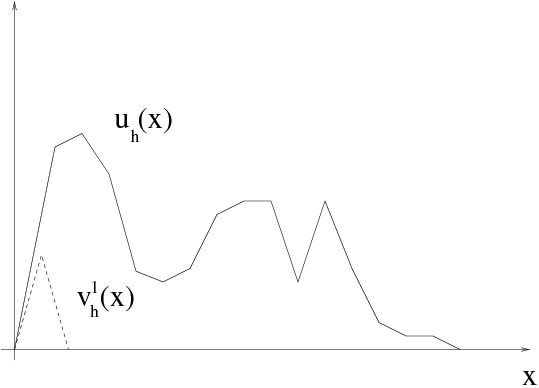
\epsfig{file={../fig/approxesp},width=6 cm,angle=-90}}   
 \caption{L'espace $L^2[0,1]$ peut \^etre approch\'e par des fonctions
continues par morceaux.}
 \label{figapproxesp}
\end{figure}
\end{exmp}
En pratique on tombe sur la r\'esolution de syst\`emes lin\'eaires
(lorsque $a(.,.)$ est bilin\'eaire) que l'on peut r\'esoudre par des
m\'ethodes d'analyse num\'erique classiques \cite{ma:compu:Press92}. Ces
m\'ethodes\cite{ma:equad:Ciarlet88,ma:compu:Press92,ma:compu:Nougier87}
peuvent \^etre directes 
(m\'ethode de Gauss,Cholesky) ou it\'eratives (Jacobi, Gauss-Seidel,
relaxation). 

\subsection{\'El\'ements finis}
%%%%%%%%%%%%%%%%%%%%%%%%%%%%%
Cette m\'ethode correspond aux cas des g\'eom\'etries
irr\'eguli\`eres. On choisit alors une base adapt\'ee au probl\`eme. 
Cette m\'ethode fait appel \`a une formulation variationelle.
\section{\'Evolution : Int\'egration temporelle}
%%%%%%%%%%%%%%%%%%%%%%%%%%%%%%%%
\subsection{Probl\`eme}
%%%%%%%%%%
On cherche \`a r\'esoudre le probl\`eme suivant:
\begin{prob}\label{probmathevovec}
Trouver la solution $y(x,t)$
\begin{equation}
\frac{dy}{dt}=f(y,t)
\end{equation}
ou $y$ est un vecteur \`a $N$ dimensions et $y(t=0)$ est connu
(probl\`eme de Cauchy). 
\end{prob}
Ce probl\`eme peut \^etre rencontr\'e en tant que tel dans de nombreux
probl\`emes de la physique, mais il peut aussi correspondre \`a la
discr\'etisation d'\'equation d\'evolution aux d\'eriv\'ees partielles.
Comme toujours en calcul num\'erique se pose la question de savoir
dans quelle mesure le calcul num\'erique de la solution du probl\`eme
\ref{probmathevovec} est proche de la solution math\'ematique de ce
m\^eme probl\`eme. Nous n'entrerons pas ici dans les d\'etails des
calculs de pr\'ecision et de stabilit\'e des sch\'emas
d'int\'egration, mais il faut garder toujours \`a l'esprit ce
probl\`eme crucial. Notamment, il faut autant que possible utiliser les
propri\'et\'es connues des solutions et v\'erifier que l'approximation
num\'erique v\'erifie ces m\^emes propr\'iet\'es. Par exemple si l'on
sait que la solution de probl\`eme \ref{probmathevovec} est born\'ee
dans le temps, et que la solution num\'erique explose, alors la
solution num\'erique ne sera pas une bonne approximation de la
solution exacte. Le test de la stabilit\'e est donc le premier que le
num\'ericien utilise en pratique. Mais un sch\'ema stable peut aussi
\^etre une pi\`etre approximation. Par exemple il faut tenir compte
des possibles int\'egrales du mouvement. Un syst\`eme hamiltonien
conserve l'\'energie, donc il est bon de tester sur la solution
num\'erique si son \'energie est conserv\'ee au cours du temps.
\subsection{La m\'ethode d'Euler}
%%%%%%%%%%%%%%%%%%%%%%%%%%%%%%
Une m\'ethode d'Euler simple consiste \`a approcher la d\'eriv\'ee par
rapport au temps
\begin{equation}
\frac{du_k}{dt}
\end{equation}
par
\begin{equation}
\frac{1}{\Delta t}(u_{k,t+1}-u_{k,t})
\end{equation}
Mais la m\'ethode d'\'evaluation du terme de droite est tr\`es
importante pour la stabilit\'e du sch\'ema d'int\'egration
\cite{ma:compu:Press92}. Ainsi une m\'ethode explicite du type :
\begin{equation}
\frac{1}{\Delta t}(u_{k,t+1}-u_{k,t})=F_i(u_t)
\end{equation}
n'est pas stable dans le cas ou $F=\frac{\partial u}{\partial x}$.
Par contre, la m\'ethode implicite :
\begin{equation}\label{eqimpli}
\frac{1}{\Delta t}(u_{k,t+1}-u_{k,t})=F_i(u_{t+1})
\end{equation}
est stable. N\'eanmoins, un tel sch\'ema implique que l'on sait
r\'esoudre l'\'equation \ref{eqimpli} \`a chaque pas de temps. C'est
le cas en particulier si $F$ est lin\'eaire. On peut alors appliquer
les m\'ethodes classiques de r\'esolution de syst\`eme \cite{ma:compu:Press92}.
On peut montrer que le sch\'ema dit de Cranck-Nicholson :
\begin{equation}
\frac{1}{\Delta t}(u_{k,t+1}-u_{k,t})
= \frac{1}{2}[F_i(u_{t+1})+F_i(u_{t})] 
\end{equation} 
est en fait du second ordre en temps.
Une m\'ethode souvent utilis\'ee est la m\'ethode saute-mouton
(leap-frog):
\begin{equation}
\frac{1}{2\Delta t}(u_{k,t+1}-u_{k,t-1})
=F_i(u_{t}) 
\end{equation} 
\begin{exmp}
Illustrons la m\'ethode d'Euler pour l'\'equation de Van der Pol :
\begin{equation}
\ddot{x}-\epsilon(1-x^2)\dot{x}+x=0
\end{equation}
qui peut s'\'ecrire :
\begin{eqnarray}
\frac{dx}{dt}&=&y\\
\frac{dy}{dt}&=&\epsilon (1-x^2)y-x
\end{eqnarray}
\begin{figure}[htb]
 \centerline{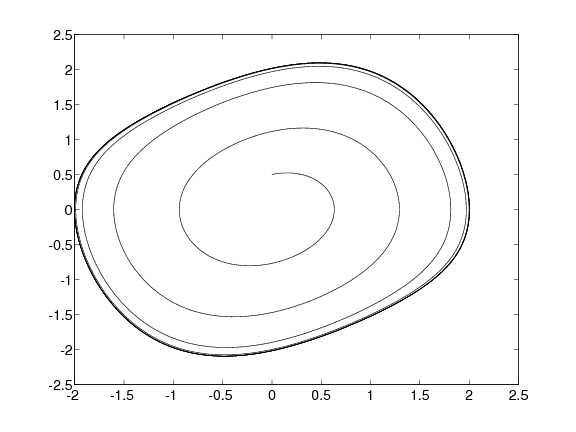
\epsfig{file={../fig/pol03i},width=6 cm}}   
 \caption{$\epsilon=0.3$, conditions initiales interieures \`a l'attracteur.}
 \label{figpol03i}
\end{figure}
\begin{figure}[htb]
 \centerline{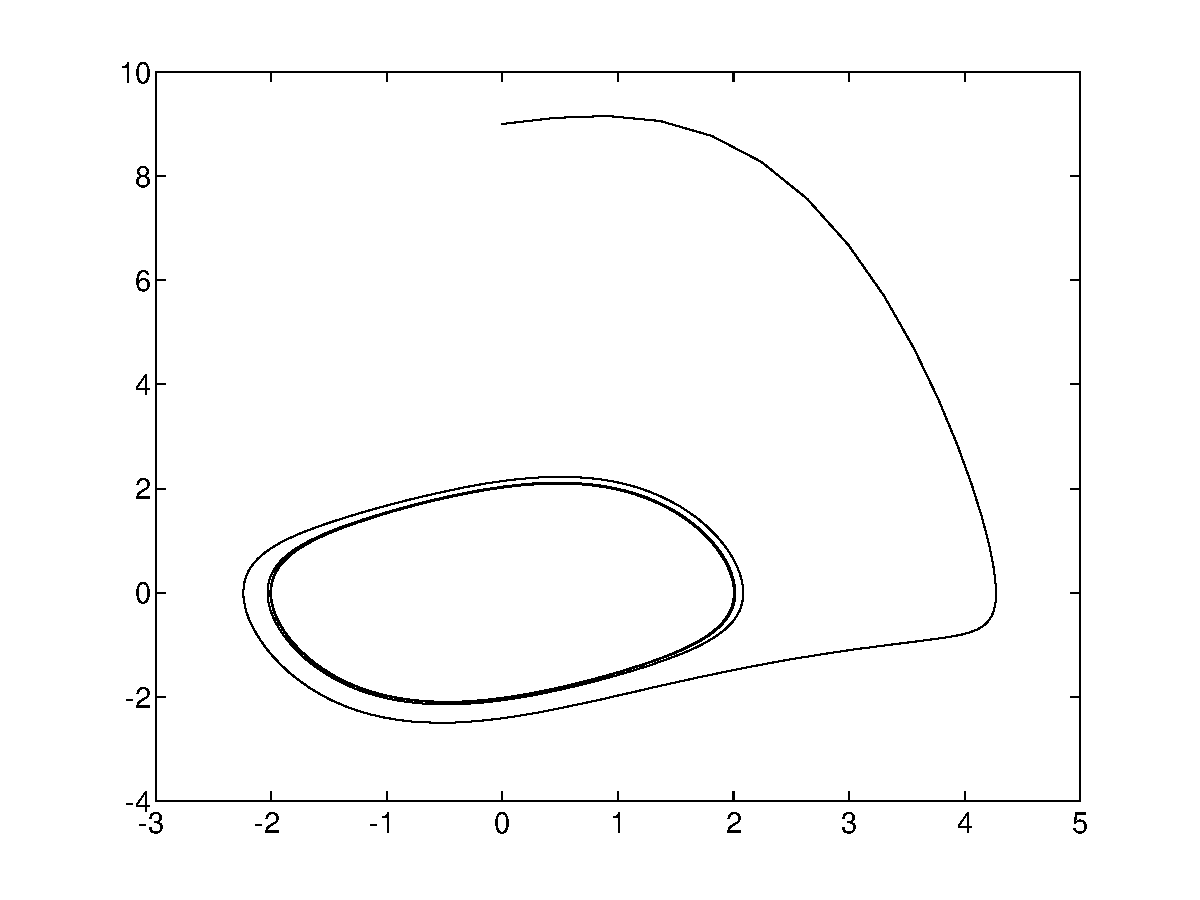
\epsfig{file={../fig/pol03e},width=6 cm}}   
 \caption{$\epsilon=0.3$, conditions initiales ext\'erieures \`a l'attracteur.}
 \label{figpol03e}
\end{figure}
%
\end{exmp}
\begin{exmp}
Consid\'erons le syst\`eme de r\'eaction diffusion\cite{ma:equad:Dardel93}
\begin{equation}
\frac{\partial u}{\partial t}=\gamma(a-bu+\frac{u^2}{\nu})+\nabla^2u
\end{equation}
\begin{equation}
\frac{\partial v}{\partial t}=\gamma(u^2-v)+d\nabla^2v
\end{equation}
La figure \ref{figreacd} montre les r\'esultats de l'int\'egration de
ce syst\`eme par une m\'ethode d'Euler 
en prenant des conditions aux limites p\'eriodiques et en utilisant un
Laplacien en diff\'erences finies. Le r\'eseau comporte
$100 \times 50$ sites.
%
\begin{figure}
\begin{tabular}[t]{cc}
\epsffile{../fig/reacdt1ga5e_04ite2}&
\epsffile{../fig/reacdt1ga5e_04ite4}\\
\epsffile{../fig/reacdt1ga5e_04ite6}&
\epsffile{../fig/reacdt1ga5e_04ite8}\\
\epsffile{../fig/reacdt1ga5e_04ite10}&
\epsffile{../fig/reacdt1ga5e_04ite12}\\
\epsffile{../fig/reacdt1ga5e_04ite14}&
\epsffile{../fig/reacdt1ga5e_04ite16}\\
\epsffile{../fig/reacdt1ga5e_04ite18}&
\epsffile{../fig/reacdt1ga5e_04ite20}\\
\end{tabular} 
\caption{Simulation du syst\`eme r\'eaction diffusion sur un r\'eseau
de $100 \times 50$ sites. Un site en noir correspond \`a une valeur de
$u$ sup\'erieure \`a la $(u_{max}-u_{min})/2$. Lorsque le temps
\'evolue, on observe la formation
de structures spatiales pouvant mod\'eliser
l'apparition des taches sur la peau de certains animaux.}
\label{figreacd}
\end{figure}
On a pris pour valeur num\'erique $\gamma=5$, $a=0.5$, $b=2$, $D=10$,
$dt=0.01$. On a pris comme condition initiale sur chaque site les
valeurs $u(i,j)=0.25+0.001*rand(i,j)$ et $v(i,j)=0.6+0.001*rand'(i,j)$
ou les $rand(i,j)$ et $rand'(i,j)$ sont des nombres al\'eatoires
compris entre $0$ et $1$. Ces conditions initiales peuvent \^etre
obtenues par l'\'etude analytique (ou num\'erique) du syst\`eme sans
diffusion. 

Un tel syst\`eme de r\'eaction diffusion permet de d\'ecrire en
particulier  les comportements spatio--temporels de syst\`emes dont
deux grandeurs $u$ et $v$ ont chacune un r\^ole diff\'erent :
la premi\`ere joue le r\^ole d'activateur, la seconde d'inhibiteur. De
tels mod\`eles peuvent par exemple 
d\'ecrire l'\'evolution d'un incendie de for\^et (l'activateur du feu
est le bois de la for\^et, l'inhibiteur est le pompier) ou l'apparition de
taches sur la peau de certains animaux (z\`ebres, gu\'epards,\dots)
ou les activateur et inhibiteur sont deux substances chimiques.

%
\end{exmp}
\begin{exmp}
Une \'equation de Klein-Gordon non lin\'eaire 
\begin{equation}
u_{xx}-u_{tt}=F(u)
\end{equation}
o\`u $F$ est (\'equation de Sine-Gordon)
\begin{equation}
F(u)=\sin u
\end{equation}
ou (phi quatre)
\begin{equation}
F(u)=-u+u^3
\end{equation}
peut \^etre int\'egr\'ee
par un sch\'ema saute mouton\cite{ma:equad:Dodd82} :
\begin{equation}
u_{t+1,k} = -u_{t-1,k}+u_{t,k+1}+ u_{t,k-1}-
h^2F[\frac{1}{2}(u_{t,k+1}+u_{t,k-1})] 
\end{equation}
\end{exmp}

\subsection{M\'ethode de Runge-Kutta}
%%%%%%%%%%%%%%%%%%%%%%
La formule de Runge-Kutta\index{Runge-Kutta} \`a l'ordre 4 exprime $y_{i+1}$ en fonction
de $y_i$ par la formule suivante : 
\begin{equation}
y_{i+1}=y_i+\frac{\Delta
t}{6}[f(y_i,t_i)+2f(yy_{i+\frac{1}{2}},t_{i+\frac{1}{2}})+
2f(yyy_{i+\frac{1}{2}},t_{i+\frac{1}{2}})+ f(yy_{i+1},t_{i+1})]
\end{equation}
o\`u
\begin{equation}
yy_{i+\frac{1}{2}}=y_i+\frac{\Delta t}{2}f(y_i,t_i)
\end{equation}
\begin{equation}
yyy_{i+\frac{1}{2}}=y_i+\frac{\Delta t}{2}f(yy_{i+\frac{1}{2}},t_{i+\frac{1}{2}})
\end{equation}
\begin{equation}
yy_{i+1}=y_i+{\Delta t}f(yyy_{i+\frac{1}{2}},t_{i+\frac{1}{2}})
\end{equation}

\subsection{M\'ethode d'Adams (\`a pas multiples)}
%%%%%%%%%%%%%%%%%%%
Le probl\`eme 
\begin{equation}
\frac{d u}{dt}=F(u)
\end{equation}
se r\'esoud par les formules suivantes :
Adams\index{Adams} ouverte \`a l'ordre 2 :
\begin{equation}
u_{i+1}=y_i+\frac{\Delta t}{2}(3F_i-F_{i-1})
\end{equation}
Adams ouverte \`a l'ordre 3 :
\begin{equation}
u_{i+1}=y_i+\frac{\Delta t}{12}(23F_i-16F_{i-1}+5F_{i-2})
\end{equation}
Les m\'ethodes d'Adams ouvertes sont \`a pas multiples : elles ne peuvent
initier un processus d'int\'egration.
Adams ferm\'ee \`a l'ordre 2 :
\begin{equation}
u_{i+1}=y_i+\frac{\Delta t}{2}(F_{i+1}+F_{i})
\end{equation}
Adams ferm\'ee \`a l'ordre 3 :
\begin{equation}
u_{i+1}=y_i+\frac{\Delta t}{12}(5F_{i+1}-8F_{i}-F_{i-1})
\end{equation}
Les m\'ethodes d'Adams ferm\'ees sont aussi \`a pas multiples.  
Elles sont plus pr\'ecises mais elles sont implicites. Elles
n\'ecessitent donc la r\'esolution d'un syst\`eme d'\'equation \`a
chaque pas de temps. La m\'ethode du pr\'edicteur--correcteur fournit
un moyen pratique d'utiliser les m\'ethodes d'Adams ferm\'ees.
\subsection{M\'ethode de pr\'edicteur-correcteur}
%%%%%%%%%%%%%%%%%%%%%%%%%%%%%
Les m\'ethodes de
pr\'edicteur--correcteur\index{pr\'edicteur-correcteur} sont de
puissantes 
m\'ethodes, tr\`es utiles dans le cas o\`u le terme de droite est
complexe.
On calcule la valeur $\tilde u_{i+1}$ estim\'ee (pr\'edicteur) gr\^ace
\`a une m\'ethode d'Adams ouverte, par exemple celle d'ordre 3 :
\begin{equation}
\tilde u_{i+1}=u_i+\frac{\Delta t}{12}[23F(u_i)-16F(u_{i-1})+5F(u_{i-2})]
\end{equation}
On \'evalue \`a nouveau $u_{i+1}$ par l'approximation donn\'ee par une
formule (implicite) d'Adams ferm\'ee dans laquelle on utilise la
valeur $\tilde u_{i+1}$ 
\begin{equation}
u_{i+1}=y_i+\frac{\Delta t}{12}[5F(\tilde u_{i+1}-8F(u_{i})-F(u_{i-1})]
\end{equation}
On peut utiliser la formule pr\'ec\'edente pour \'evaluer \`a
chaque it\'eration  $F$ \`a partir de la valeur $u_{i+1}$ estim\'ee
\`a l'\'etape pr\'ec\'edente. 
\begin{rem}
C'est surtout l'\'evaluation de $F$ dans la formule implicite qui
stabilise le sch\'ema. Ainsi un probl\`eme :
\begin{equation}
\frac{du}{dt}=Lu+N(u)
\end{equation}
o\`u $L$ est un op\'erateur lin\'eaire et $N$ un op\'erateur
non--lin\'eaire pourra \^etre avantageusement abord\'e par le sch\'ema
pr\'edicteur--correcteur suivant :
\begin{equation}
\tilde u_{i+1}=\exp(L.\Delta t)u_i+\Delta t N(u_i)
\end{equation}
\begin{equation}
u_{i+1}=\exp(L.\Delta t)u_i+\Delta t N(\frac{\tilde u_{i+1}+u_i}{2})
\end{equation}
\end{rem}

\subsection{Cas particulier des transformations symplectiques}
%%%%%%%%%%%%%%%%%%%%%%%%%%%%%%%%%%%%%
Envisageons\index{sympl\'ectiques} un cas particulier du probl\`eme
\ref{probmathevovec} : 
\begin{prob}
Trouver la solution $[q(t),p(t)]$
\begin{equation}
\frac{dq}{dt}=f(q,p)
\end{equation}
\begin{equation}
\frac{dp}{dt}=g(q,p)
\end{equation}
o\`u $[q(t=0),p(t=0)]$ est connu (probl\`eme de Cauchy) et o\`u les
fonctions $f$ et $g$ d\'erivent d'un hamiltonien $H(q,p)$:
\begin{equation}
f=\frac{\partial H}{\partial p}
\end{equation}
\begin{equation}
g=-\frac{\partial H}{\partial q}\\
\end{equation}
\end{prob}
Ce cas correspond au cas o\`u le volume $dq.dp$ est conserv\'e.
Introduisons dans le
cas discret une transformation $T$ symplectique :
\begin{defn}
Une transformation T d\'efinie par :
\begin{eqnarray}
q_{n+1}&=&f(q_n,p_n)\\
p_{n+1}&=&g(q_n,p_n)
\end{eqnarray}
est symplectique si la jacobienne de T est de d\'eterminant 1.
\end{defn}
Pr\'esentons deux m\'ethodes symplectiques :
\begin{rem}
La m\'ethode d'Euler n'est pas symplectique :
\begin{eqnarray}
q_{n+1}&=&q_n+V(p_n)\delta t\\
p_{n+1}&=&p_n+F(q_n)\delta t
\end{eqnarray}
\end{rem}
\begin{exmp}
Verlet symplectique ordre 1
\begin{eqnarray}
q_{n+1}&=&q_n+V(p_n)\delta t\\
p_{n+1}&=&p_n+F(q_{n+1})\delta t
\end{eqnarray}
\end{exmp}
\begin{exmp}
Staggered scheme (saute mouton-rectifie) symplectique ordre 2
\begin{eqnarray}
\frac{1}{\delta t}(p_{n+1}-p_{n})&=&F(q_{n+\frac{1}{2}})\\
\frac{1}{\delta t}(q_{n+1+\frac{1}{2}}-q_{n+\frac{1}{2}})&=&V(P_{n+1})
\end{eqnarray}
\end{exmp}
Les trois figures suivantes repr\'esentent la trajectoire calcul\'ee
par les trois m\'ethodes Euler, Verlet et Verlet rectifi\'ee pour le
syst\`eme (lin\'eaire) qui d\'ecrit l'oscillateur harmonique :
\begin{equation}
\left\{ \begin{array}{lcr}
\dot x&=&-y\\
\dot y&=&x
\end{array}\right.
\end{equation}
\begin{figure}[tbh]
\centerline{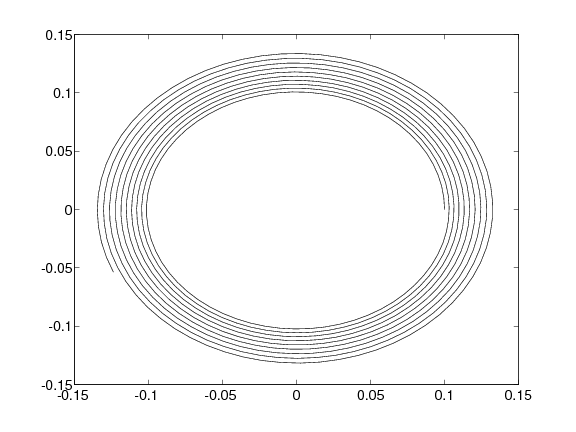
\epsfig{file={../fig/EulerOscillo001},width=6 cm}}
\caption{\it M\'ethode d'Euler avec un pas $h=0.01$ pour l'oscillateur harmonique. }
\label{codefigure1}
\end{figure}
%
\begin{figure}[tbh]
\centerline{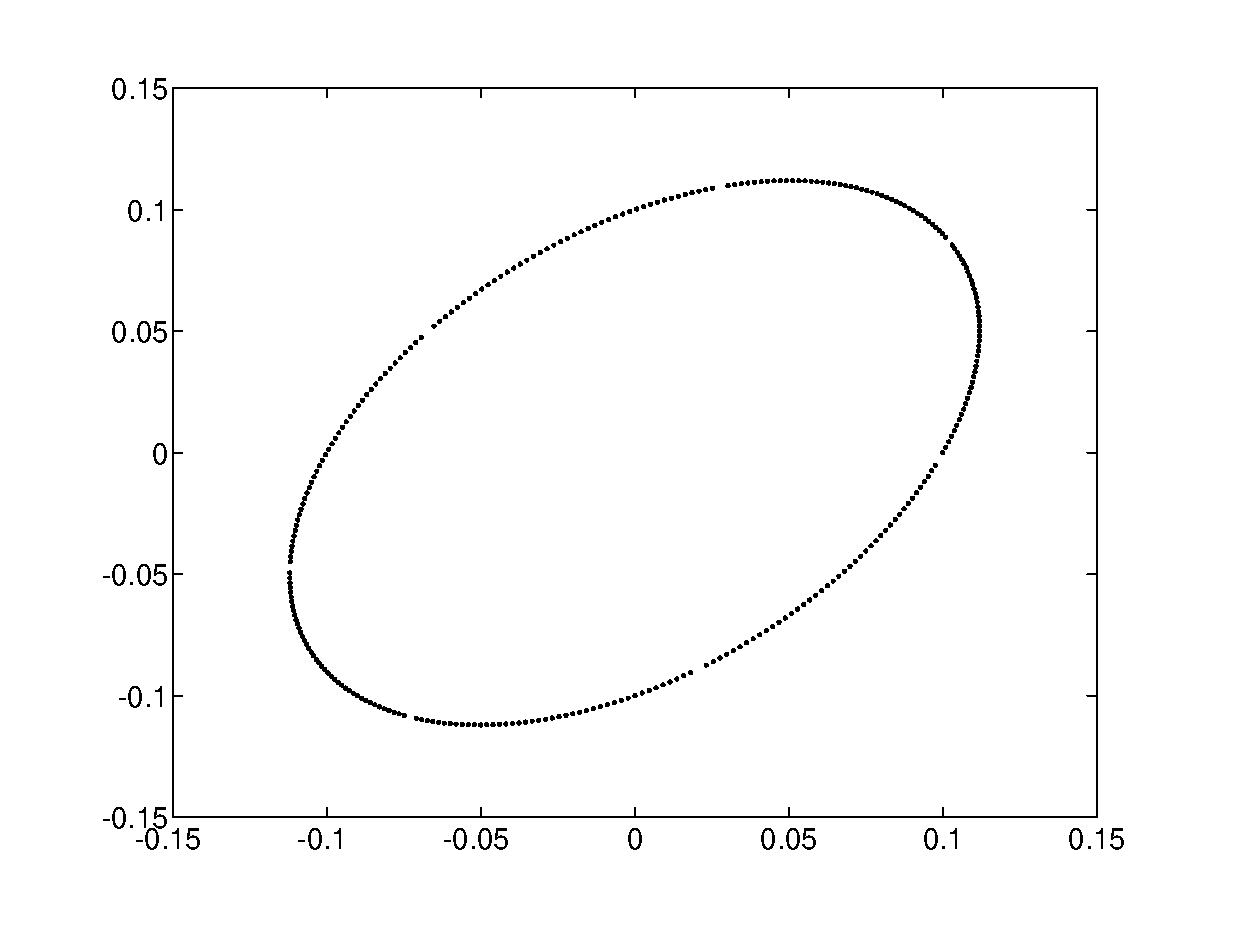
\epsfig{file={../fig/VerletOscillo1},width=6 cm}}   
\caption{\it M\'ethode de Verlet avec un pas de $h=0.9$ pour l'oscillateur
  harmonique. Malgr\'e un pas de temps sup\'erieur \`a celui utilis\'e avec la
  m\'ethode d'Euler, l'\'energie est conserv\'ee avec une bonne approximation.}
\label{codefigure2}
\end{figure}
%
\begin{figure}[tbh]
\centerline{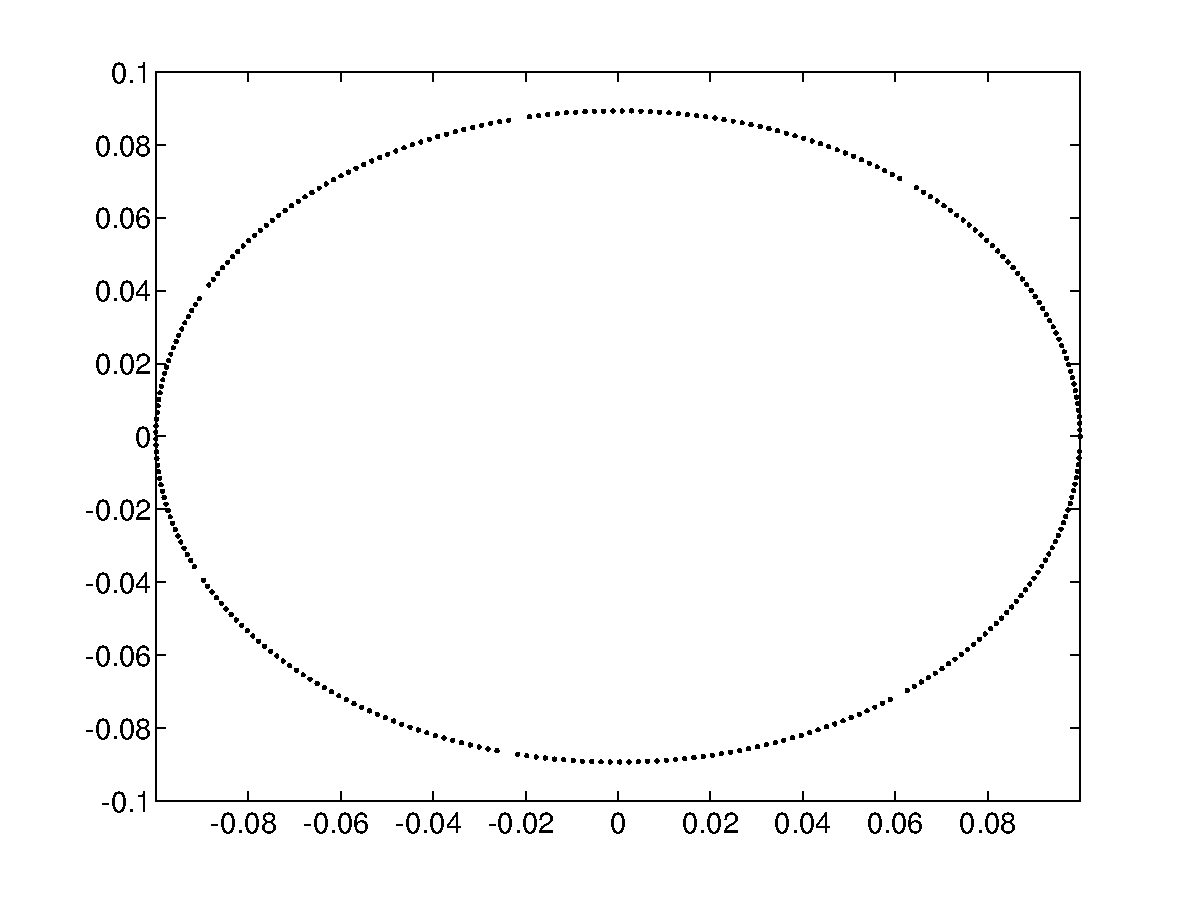
\epsfig{file={../fig/VerletRecOscillo09},width=6 cm}}   
\caption{\it M\'ethode de Verlet rectifi\'e avec un pas de $h=0.9$ pour
  l'oscillateur harmonique. L'\'energie reste conserv\'ee et l'espace des
  phases est moins d\'eform\'e.}
\label{codefigure3,}
\end{figure}
%
\section{Autres probl\`emes}
%%%%%%%%%%%%%%%%%%%%%%%%%%
\subsection{\'Equations aux d\'eriv\'ees partielles : probl\`emes aux
limites} 
%%%%%%%%%%%%%%%%%%%%%%%%%%%%%%
Ces probl\`emes se r\'eduisent en g\'en\'eral \`a la r\'esolution de
grands syst\`emes d'\'equations \cite{ma:compu:Press92}. Pour les diff\'erentes
m\'ethodes (relaxation, rapide, directe) voir \cite{ma:compu:Press92,ma:equad:Ciarlet88}
\subsection{\'Equations aux d\'eriv\'ees partielles : probl\`emes
spectraux}  
%%%%%%%%%%%%%%%%%%%%%%%%%%%%%%
Le probl\`eme spectral est aussi un des probl\`emes fr\'equemment
rencontr\'e en physique. Notamment, lors de la r\'esolution de
probl\`eme d'\'evolution par la m\'ethode spectrale. Nous renvoyons aux
ouvrages cit\'es pr\'ec\'edemment \cite{ma:compu:Press92,ma:compu:Nougier87}.
\subsection{Calculs de physique statistique}
%%%%%%%%%%%%%%%%%%%%%
En physique statistique, l'\'evaluation des moyennes et grandeur se
fait avantageusement par des m\'ethodes de Monte-Carlo. Nous
pr\'esentons ici un exemple simple de calcul.
\begin{exmp}
Envisageons le
cas particulier du mod\`ele d'Ising.
Dans un syst\`eme de spin, l'\'energie du syst\`eme s'\'ecrit:
\begin{equation}
E=-J\sum_i\sum_k S_iS_k-B\sum S_k
\end{equation}
L'algorithme de Metropolis\cite{ma:compu:Stauffer93,ma:compu:Koonin90}
est utilis\'e\index{M\'etropolis} 
pour simuler les probabilit\'es $exp(-E/k_BT)$ :
\begin{enumerate}
\item s\'electionner un spin $S_k$ \`a \'etudier
\item calculer la variation d'\'energie $\Delta E=E_{nouv}-E_{ancien}$
associ\'ee \`a un possible retournement du spin $S_k$.
\item comparer un nombre tir\'e  au hasard $z$, avec $0<z<1$, avec la
probabilit\'e $p=exp(-\Delta E/k_BT)$.
\item tourner le spin $S_k=-S_k$ si et seulement si $z<p$.
\item utiliser la pr\'esente configuration pour calculer toute moyenne.
\end{enumerate}
\end{exmp}


\def\exoscorr{%%%%%%%%%%%%%%%%%%%%%%%%%%%%%%%%%%%
\chapter{Solution des exercices}

Solution de l'exercice \ref{exoentr}

En annulant la quantit\'e $dL=dS+\sum_{i=0}^{n} \lambda_iR_i$, on obtient
le syst\`eme :
\begin{equation}
\frac{\partial L}{\partial P_l}=-k_B(\ln P_l+1)-\lambda_1-\sum_{i=1}^n\lambda_iX^i_l
\end{equation}
ce qui donne 
\begin{equation}
P_l=e^{-1-\frac{1}{k_B}(\lambda_1+\sum \lambda_i X^i_l)}
\end{equation}
Dans le cas particulier o\`u aucune moyenne n'est impos\'ee (on a
seulemet $R_1$ comme contrainte) alors la probabilit\'e $P_l$ devient :
\begin{equation}
P_l=\frac{1}{N}
\end{equation}
o\`u $N$ est le nombre d'\'etats : tous les \'etats sont
\'equiprobables. 



Solution de l'exercice \ref{exospectramatrice}

Soit $L$ est un op\'erateur lin\'eaire et $X$ un vecteur d'un espace
de dimension finie $n$
d\'eterminant l'\'etat du syst\`eme physique \`a l'instant $t$.
Consid\'erons le probl\`eme suivant :
\begin{prob},
Trouver $X$ tel que :
\begin{equation}\label{eqevol2}
\frac{dX}{dt}=L X
\end{equation}
et
\begin{equation}
X(0)=X_0
\end{equation}
\end{prob}
La solution de ce probl\`eme est connue :
On diagonalise $L$ (si $L$ est sym\'etrique- ou autoadjoint-
, alors $L$ est diagonalisable)
et dans la base des vecteurs propres $e_k$, le syst\`eme devient :
\begin{equation}
\frac{dy_k}{dt}=\lambda_ky_k
\end{equation}
o\`u $\lambda_k$ est la $k^{\grave{e}me}$ valeur propre et $y_k$ la composante
sur le vecteur propre $e_k$.
\begin{rem}
Le probl\`eme :
\begin{prob}
Trouver $X$ tel que :
\begin{equation}\label{eqevolv}
\frac{d^2X}{dt^2}=L X
\end{equation}
et
\begin{equation}
X(0)=X_0
\end{equation}
et
\begin{equation}
\frac{dX}{dt}(0)=\dot{X}_0
\end{equation}
\end{prob}
se ram\`ene au probl\`eme pr\'ecedent en introduisant le vecteru
$Y=(X,\frac{dX}{dt}$) et l'op\'erateur 
\begin{equation}
M=
\left( \begin{array}{cc}
0 &I\cr
 L & 0
\end{array} \right)
\end{equation}
\end{rem}
Il existe de tr\`es nombreux exemples de syst\`emes physiques qui
poss\`edent une \'equation de la forme \ref{eqevol,v}
\begin{exmp}
Cha\^\i nes d'oscillateurs coupl\'es.
L'\'equation r\'egissant l'\'evolution d'un syst\`eme de deux
oscillateurs coupl\'es  est :
\begin{equation}
\ddot x_1=-\frac{k}{2m}x_1+\frac{k}{m}x_2
\end{equation}
\begin{equation}
\ddot x_2=+\frac{k}{m}x_1-\frac{k}{2m}x_2
\end{equation}
o\`u $x_1$ et $x_2$ sont les \'ecarts par rapport \`a la position
d\'equilibre. 
\end{exmp}


Correction de l'exercice \ref{exocordespec}

Le cas de la corde vibrante peut \^etre abord\'e de cette \^etre
car l'op\'erateur $L$ est invariant par translation donc diagonalisable
par transformation de Fourier.
Consid\'erons l'\'equation des ondes qui d\'ecrit par exemple les
vibrations 
transverses d'une corde.
\begin{equation}
\frac{\partial^{2}}{\partial
x^{2}}u(x,t)=\frac{1}{c^2}\frac{\partial^{2}}{\partial t^{2}}u(x,t)
\end{equation}
Nous nous fixons des conditions aux limites de type :
\begin{equation}
{\rm (CL}_1{\rm)\ }u(0,t)=0,\:u(l,t)=0
\end{equation}
ou
\begin{equation}
{\rm (CL}_1{\rm)\ }\frac{\partial}{\partial
x}u(0,t)=0,\:\frac{\partial}{\partial x}u(l,t)=0 
\end{equation}
Les conditions aux limites CL$_1$ correspondent au cas o\`u la corde est
fix\'ee en $0$ et en $l$.
Les conditions aux limites CL$_2$ correspondent au cas o\`u la corde est
libre de glisser en $0$ et en $l$ tout en gardant une pente
horizontale en ces points.
Nous nous donnons aussi des conditions initiales :
\begin{equation}
u(x,0)=u^1(x),\:\frac{\partial}{\partial t}u(x,0)=u^2(x)
\end{equation}
Cherchons les fonctions propres $e_{i}(x)$ de l'op\'erateur $\frac{\partial^{2}}{\partial x^{2}}$. Les $e_{i}(x)$ v\'erifient :
\begin{equation}
\frac{\partial^{2}}{\partial x^{2}} e_{i}(x)= a_{i} e_{i}(x)
\end{equation}
D\'eveloppons $u(x,t)$ sur la base des fonctions propres $e_{i}(x)$ de
l'op\'erateur $\frac{\partial^{2}}{\partial x^{2}}$. Le spectre est
discret.
En portant ce d\'eveloppement dans l'\'equation r\'egissant la
dynamique, on obtient un syst\`eme d'\'equations portant sur les
d\'eriv\'ees temporelles des coefficients du d\'eveloppement.
\begin{rem}
Au lieu de diagonaliser l'op\'erateur $\frac{\partial^{2}}{\partial
x^{2}}$ agissant sur les fonctions de $x$ ont peut diagonaliser
l'op\'erateur d\'eriv\'ee seconde par rapport au temps.
$\frac{\partial^{2}}{\partial t^{2}}$.Cet op\'erateur est invariant
par 
translation dans le temps. On sait\footnote{\`a voir} que la
transformation de Fourier ou de Laplace diagonalise l'op\'erateur.
\end{rem}
\begin{rem}
Une m\'ethode un peut plus artificielle est d'utiliser un d\'eveloppement
en s\'erie de Fourier en $x$. (voir \cite{ma:equad:Dautray7} t7p217, 223)
Pour les CL$_1$ on r\'esout le probl\`eme dans la base des fonctions
impaires de p\'eriode $2l$.
Pour les CL$_1$ on r\'esout le probl\`eme dans la base des fonctions paire
de p\'eriode $2l$.
\end{rem}



Correction de l'exercice \ref{exopoincalin}.

Introduisons la fonction :
\begin{equation}
G(u,\omega)=\left[\omega^2\partial_{\tau}\partial_{\tau}-\partial_{x}\partial_{x}\right]u-f(u)
\end{equation}

{\bf Ordre z\'ero :}%%%%%%%%
En portant le d\'eveloppement de $u$ dans  \ref{fix} et en faisant 
 $\epsilon=0$ on trouve que 
$u_0(x)=0$ est la solution \`a l'ordre 0.

{\bf Premier ordre :}%%%%%%%
D\'erivons donc $G(u,\omega)$ par rapport \`a $\epsilon$ 
et faisons $\epsilon=0$.
\begin{equation}
\left.\frac{\partial G}{\partial u}\right\rfloor_{\epsilon
=0}\left.\frac{\partial u}{\partial \epsilon}\right\rfloor_{\epsilon
=0}+ \left.\frac{\partial G}{\partial \omega}\right\rfloor_{\epsilon
=0}\left. \frac{\partial \omega}{\partial
\epsilon}\right\rfloor_{\epsilon =0}=0 
\end{equation}
D'o\`u :
\begin{equation}
\left.\frac{\partial G}{\partial u}\right\rfloor_{\epsilon =0}u_1+\left.\frac{\partial G}{\partial \omega}\right\rfloor_{\epsilon =0}\omega_1=0
\end{equation}
En d\'erivant (\ref{fix}) par rapport \`a $\omega$ et 
en faisant $\omega=\omega_0$ et $\epsilon=0$ on obtient
\begin{equation}
\left.\frac{\partial G}{\partial \omega}\right\rfloor_{\epsilon=0}=0
\end{equation}
Nous obtenons donc \`a l'ordre 1 :
\begin{equation}
\left.\frac{\partial G}{\partial
\omega}\right\rfloor_{u_0,\omega_0}u_1(x,\tau)=0
\label{ord1}
\end{equation}
Comme
\begin{equation}
G(u,\omega)=\left[\omega^2\partial_{\tau}\partial_{\tau}-\partial_{x}\partial_{x}\right]-f(u),
\end{equation}
l'\'equation (\ref{ord1}) s'\'ecrit ici :
\begin{equation}
\left[\omega^2_0\partial_{\tau}\partial_{\tau}-\partial_{x}\partial_{x}-f'(0)\right]u_1(x,\tau)=0
\end{equation}
%%%%%%%%%%%%%%%%%%%%%%%%%%%%%%%%%%%%%%%%%%%%%%%%
% fonction impaire
%%%%%%%%%%%%%%%%%%%%%%%%%%%%%%%%%%%%%%%%%%%%%%%%
D'apr\`es les conditions aux limites :
\begin{equation}
u(0,\tau)=u(\pi,\tau)=0
\end{equation}
Nous pouvons d\'ecomposer en s\'erie de Fourier :
\begin{equation}
u(x,\tau)=\sum_k u_k(t) \sin kx
\end{equation}
o\`u $k$ est un entier.
Ensuite, comme on a impose la p\'eriodicit\'e :
\begin{equation}
u(x,\tau+\pi)=u(x,\tau)
\end{equation}
L'\'equation v\'erifi\'ee par $u_{k,1}(\tau)$ est :
\begin{equation}
\left[\omega^2_0\partial_{\tau}\partial_{\tau}+k^2-f'(u)\right]u_{k,1}(\tau)=0
\end{equation}
on peut d\'evelopper en s\'erie de Fourier chaque $u_{k,1}(\tau)$.
On trouve comme condition :
\begin{equation}
\omega_0^2=\frac{k^2-f'(0)}{n^2}
\end{equation}
et
\begin{equation}
u_{k,1}(x,\tau)=\sin(kx)(A\cos n\tau-B\sin n\tau)
\end{equation}
{\bf Conditions aux limites}
%%%%%%%%%%%%%%%%%%%%%%%%%%%%%%%
Nous imposons 
\begin{equation}
u(x=0,\tau)=u(x=1,\tau)=0
\end{equation}
Donc nous pouvons d\'evelopper $u(x,\tau)$ sur la base des sinus :
\begin{equation}
u(x,\tau)=\sum_k u_{k}(\tau) \sin kx
\end{equation}
De m\^eme nous pouvons d\'evelopper les $u_i(x,\tau)$ :
\begin{equation}
u_i(x,\tau)=\sum_k u_{ik}(\tau) \sin kx
\end{equation}
D'autre part nous avons suppose la p\'eriodicit\'e en $\tau$ donc :
\begin{equation}
u_{ik}(\tau)=\sum_n u_{ikn}\cos n\tau
\end{equation}
en supposant les conditions initiales :
\begin{equation}
\frac{\d u_{ik}}{d \tau}(\tau=0)=0
\end{equation}
\begin{equation}
u_{ikn}(\tau=0)=u_{ikn}
\end{equation}
Chaque $u_i$ s'\'ecrit donc :
\begin{equation}
u_i(x,t)=\sum_k\sum_n u_{ikn}\sin kx \cos n\omega(k,n,\epsilon)t
\label{devui}
\end{equation}
Pas vrai pour $i\rangle 1$
A l'ordre 1 nous avons donc :
\begin{equation}
u_i(x,t)=\sum_k\sum_n u_{ikn}\sin kx \cos \Omega_kt
\end{equation}
avec 
\begin{equation}
\Omega_k^2=k^2-f'(0)
\end{equation}
C'est ce que nous appelons une {\it relation de dispersion}.
\begin{rem}
Nous cherchons une solution p\'eriodique. Il nous faut donc fixer $k$ et
$n$.
\end{rem}
{\bf Calcul du deuxi\`eme ordre}
%%%%%%%%%%%%%%%%%%%%%%%%%%%%%%%%
En d\'erivant deux fois par rapport \`a $\epsilon$ l'\'equation et en
faisant $\epsilon=0$, on obtient :
\begin{equation}
\left[\omega^2_0\partial_{\tau}\partial_{\tau}
-\partial_{x}\partial_{x}-f'(0)\right]u_2(x,\tau) 
=f''(0)u_1^2-2\omega^2_1 u_{1,\tau\tau}
\end{equation}
Nous pouvons d\'evelopper $u_2$ d'apr\`es (\ref{devui}) :
\begin{equation}
u_2(x,t)=\sum_k\sum_n u_{2kn}\sin kx \cos n\omega(k,n,\epsilon)t
\end{equation}
Si on prend $u_1(x,\tau)=Ae^{ikx+in\tau}$ et si on suppose :
\begin{equation}
u_2(x,\tau)=\sum_q\sum_mu_{2qm}e^{iqx+im\tau}
\end{equation}
\begin{eqnarray}
\lefteqn{\sum_q\sum_m\left[-\omega^2_0(k,n)m^2+
q^2-f'(0)\right]u_{2qm}e^{iqx+im\tau}=}\nonumber\\ 
 & & \mbox{\ \ \ \ \ \ \ }f''(0)A^2e^{i2kx+i2n\tau}-
2\omega^2_1(-n^2)Ae^{ikx+in\tau} 
\\ \end{eqnarray}
En projetant sur $e^{ikx+in\tau}$ on voit que l'on doit avoir
$\omega^2_1=0$. $u_{2qm}$ est alors quelconque (CI).
En projetant sur $e^{i2kx+i2n\tau}$ 
\begin{equation}
\left[-\omega^2_0(k,n)(2n)^2+(2k)^2-f'(0)\right]u_{2,2n,2k}e^{i2kx+
i2n\tau}=f''(0)A^2e^{i2kx+i2n\tau} 
\end{equation}
D'o\`u :
\begin{equation}
u_{2,2n,2k}=f''(0)A^2/\left[-\omega^2_0(k,n)(2n)^2+(2k)^2-f'(0)\right]
\end{equation}
\begin{rem}
C'est un probl\`eme spectral pour lequl on n'a pas le choix sur les
conditions 
initiales des vecteur perturb\'es. On obtient successivement les
approximations d'une solution.  
\end{rem}



Correction de l'exercice \ref{exoplasmapert}

Un calcul \`a l'ordre z\'ero montre que si l'on n\'eglige 
 l'inertie de \'electrons  ($n^0_e m_e(\frac{\partial v^0_e}{\partial t}+({v}^0_e.\nabla v^0_e))=0$)
alors, l'\'equation de conservation de la
quantit\'e de mouvement des \'electrons projet\'ee sur le plan
perpendiculaire \`a $B$ est :
\begin{equation}
0=en^0v_e^0\wedge B +k_B T_e^0\nabla n^0.
\end{equation}
D'o\`u en multipliant vectoriellement par $B$ :
\begin{equation}\label{eqformulevit}
v_{e,\perp}^0=-\frac{k_B T_e^0 \nabla_r n^0}{e B n^0} e_\theta,
\end{equation}
o\`u $e_\theta$ est le vecteur polaire de la base $(e_r,e_\theta,e_z)$.
L'expression de $v_{i,\perp}^0$ s'obtient de la m\^eme mani\`ere, mais
si on suppose le fluide d'ions froid ($T_i^0=0$) alors $v_{i,\perp}^0=0$ : le
fluide d'ions ne tourne pas. 
La conservation
 de la quantit\'e de mouvement pour le fluide d'ions donne
au premier ordre :
\begin{equation}
m_i\tilde{n}\frac{d\tilde{v}_{i,\perp}}{dt} =
q\tilde{n}_{i,\perp}(\tilde{E}_{\perp}+\tilde{v}_{i,\perp}\wedge B). 
\end{equation}
Dans le cas o\`u l'on peut n\'egliger la d\'eriv\'ee particulaire
$\frac{d}{dt}$, la perturbation de la vitesse ionique perpendiculaire
est :
\begin{equation}
\tilde{v}_{i,\perp}=\frac{\tilde{E}_\perp\wedge B}{B^2}.
\end{equation}
L'\'equation de continuit\'e pour le fluide d'ions s'\'ecrit :
\begin{equation}\label{eqcontele}
\frac{\partial\tilde{n}/n^0}{\partial
t}+\tilde{v}_\perp\frac{\nabla_\perp{n^0}}{n^0}=0,
\end{equation}
en supposant que le terme $\tilde{v}_\perp\frac{\nabla_\perp{n_0}}{n^0}$
l'emporte sur les autres termes de la divergence.
Une relation entre le potentiel
\'electrique $\tilde{\phi}$ et
$\tilde{n}$ s'obtient par 
l'\'equation de la dynamique parall\`ele des \'electrons \cite{ph:plasm:Chen84}. 
Les \'electrons ob\'eissent
\`a la relation de Boltzmann
\begin{equation}\label{eqbold}
\frac{\tilde{n}}{n_0}=\frac{e\tilde{\phi}}{k_B T_e}.
\end{equation}
L'\'equation d\'ecrivant la dynamique du potentiel \'electrique
$\tilde{\phi}$ est, en combinant les \'equations \ref{eqcontele} et
\ref{eqbold} 
\begin{equation}
\frac{\partial \tilde{\phi}}{\partial
t}=\frac{k_B T_e\nabla_\perp\tilde\phi\wedge B}{e
B^2}.\frac{\nabla_\perp n^0}{n^0}. 
\end{equation}
En supposant que le gradient de $n^0$ est dirig\'e suivant $e_r$, le
produit scalaire pr\'ec\'edent se simplifie, et l'on obtient :
\begin{equation}
\frac{\partial \tilde{\phi}}{\partial
t}=\frac{k_B T_e\partial_\theta\tilde\phi\wedge
B}{r e B^2}.\frac{\partial_r n^0}{n^0}.
\end{equation}
C'est l'\'equation de la dynamique des fluctuations de $\phi$.



}%%%%%%%%%%%%%%%%%%%%%%%%%%%%%%%%%%%%%%%%%%%%%%%%%%
\addcontentsline{toc}{chapter}{Bibliographie}

\bibliographystyle{alpha}
\bibliography{physicsresu}
\addcontentsline{toc}{chapter}{Index}

%\input resu.ind

\end{document}




\end{document}

